% Contains everything.
% Useful for getting cross-chapter references right when texing a single chapter.

\documentclass[twoside]{report}
\usepackage{thesis}
\begin{document}
\selectlanguage{english}

\pagenumbering{roman}

\selectlanguage{english}
\newcommand{\engtitle}{Proxima}
\newcommand{\engsubtitle}{A~presentation-oriented~editor\\
for~structured~documents}

\newcommand{\nltitle}{Proxima}
\newcommand{\nlsubtitle}{Een~presentatiegerichte~editor\\
voor~gestructureerde~documenten}

\thispagestyle{empty}

\parbox{141mm}{
\begin{center}
  {\sffamily\bfseries\Huge\engtitle\\
  \vspace{0.1cm}
  \huge\engsubtitle\\}
  \vspace{1cm}
  \selectlanguage{dutch}
  {\sffamily\huge\nltitle\\
  \vspace{0.1cm}
  \LARGE\nlsubtitle\\}
%  \vspace{2cm}
%  {\sffamily\bfseries\Huge\engtitle\\}
%  \vspace{1cm}
%  \selectlanguage{dutch}
%  {\sffamily\Large\nltitle\\}
  
  \bc \vspace{4mm}
   (met een samenvatting in het Nederlands)  \\
  \vspace{1.9cm} \ec
  \vspace{2.2cm}%    spacing without "samenvatting"
  {\sffamily\Large PROEFSCHRIFT\\}
  \vspace{2.2cm}%    spacing without "samenvatting"
  \bc \vspace{1.8cm} \ec
  ter verkrijging van de graad van\\
  doctor aan de Universiteit Utrecht\\
  op gezag van de Rector Magnificus, Prof.\,Dr.~W.\,H.~Gispen,\\
  ingevolge het besluit van het College voor Promoties\\
  in het openbaar te verdedigen\\
  op vrijdag 15 oktober des middags te 12.45 uur\\
\bc
  ter verkrijging van de graad van\\
  doctor aan de Universiteit Utrecht\\
  op gezag van de Rector Magnificus, Prof.\,Dr.~W.\,H.~Gispen\\
  ingevolge het besluit van het College voor Promoties\\
  in het openbaar te verdedigen\\
  op vrijdag 15 oktober des middags te 12.45 uur\\ \ec
  \vspace{1.1cm} % was 2cm
  door\\
  \vspace{1.1cm} % was 2cm
  {\sffamily\Large Martijn Michiel Schrage\\}
  \vspace{1cm}
  geboren op 4 juni 1973, te Veendam
\end{center}
}

\clearpage
\thispagestyle{empty}
\marginpar{\parbox{147mm}{
\begin{tabular}[t]{ll}
promotores:
 & Prof.\,Dr.~S.\,D.~Swierstra\\ 
 & Prof.\,Dr.~J.\,Th.~Jeuring\\
 & Prof.~L.\,G.\,L.\,T.~Meertens\\
% &  Instituut voor Informatica en Informatiekunde, Universiteit Utrecht
\\
\multicolumn{2}{l}{Instituut voor Informatica en Informatiekunde, Universiteit Utrecht}\\
\end{tabular}
}}

\vfill

% ?? LaTeX warns that a marginpar on this page is removed (2x).

\marginpar{\parbox{147mm}{
\vspace{-4.1in}
\hspace{-1.2mm}\epsfbox{Pics/ipalogo.ps}
\vspace{.2in}

%\begin{figure}[h]
%
\epsfig{file=Pics/ipalogo.eps,bbllx=90,bblly=230}
%\end{figure}


\begin{tabular}{l}
The work in this thesis has been carried out under the auspices of the research\\
school IPA (Institute for Programming research and Algorithmics).\\
\\
ISBN 12-345-6789-0\\
\end{tabular}}}
\selectlanguage{english}

\chapter*{Preface}
\thispagestyle{empty}             % no page number in foot
\addcontentsline{toc}{chapter}{Preface}


No preface yet.
\tableofcontents

\clearpage
\pagenumbering{arabic}

\setcounter{chapter}{0} \chapter{Introduction} \label{chap:introduction}


%{\em *** Version: \today~ ***}


Many software applications involve some form of editing: a user views a data structure and provides edit gestures in order to modify this data structure. Different kinds of documents require different ways of editing, and hence a multitude of editors exists, each having its own specific edit model and user-interface conventions. Moreover,  since application designers have different ideas on what constitutes a pleasant edit model, even editors for the same document type may show significantly different edit behavior. Nevertheless, the core edit behavior, whether performed in a word-processor or a spreadsheet, is largely similar: document fragments may be copied and pasted, and new parts of the document may be constructed by selecting from menus or entering text. 

% Although gradually, the edit model and user interface of editors seems to become more standard,
% still many differences exist

An obvious research question is to abstract from the specific aspects of each editor and construct a generic system that can be instantiated to a specific editor application. Building an editor with such a system would require only a fraction of the amount of engineering required to build an editor from scratch. 
% And easy to customize. 
A generic editor enhances consistency between editors, because all instantiated editors share the same edit model, and, furthermore, it facilitates the integration of editors for different document types.


%easy to maintain and develop (features added to generic editor
% work in all applications)..

%(also say a gen editor makes it possible to build editors you wouldn't even
% think of building by hand?)

Especially in the nineteen-eighties, many research projects on structure editing were started. However, the editors developed were generally perceived as being overly restrictive, and attempts at developing less restrictive systems resulted mainly in text-only editors. Further, regardless of the restrictiveness of the edit model, the applicability of the generic editors was generally limited to source editors for programming languages and simple word-processing applications.
%No generic editor However, no editor gained much popularity . either  applicable or perceived as restrictive.  but not %one has gained widespread acceptance.
In the years following, research interest in structure editing steadily declined, and many of the generic editors that were developed are now used only for educational purposes at the institute of origin.
%Nowadays, the term structure editor even has a rather negative connotation.

In our opinion, the problem with most of these structure editors is that they either focus on editing the document structure, or the presentation (often just text).
%Lambert: (maar welke structuur-editors focussen op de presentatie en niet op de structuur??)
The document-oriented editors may have a powerful presentation mechanism, but poor editing support in the presentation, which results in a restrictive edit model. On the other hand,  purely presentation-oriented editors lack edit operations on the document, and have relatively weak presentation mechanisms.

% ample support? geeft wel dubbele "there is"
With the increasing popularity of the XML format for representing structured documents, the advantages of a powerful generic editor are becoming even more apparent. Many XML document types are being developed, but support for editing documents of these types is still poor. 
There is a choice between using an expensive custom-made editor, or a generic XML editor, but the functionality of the latter does not come close to what a presentation-oriented (WYSIWYG) editor could potentially offer. It is, for instance, not possible to use any of the current XML editors as a convenient editor for a programming language or for mathematical equations.

In this thesis we investigate whether and how the advantages of structure editing and a powerful presentation formalism can be combined with a non-restrictive presentation-oriented edit model. The result of this research is the presentation-oriented structure editor Proxima.
Before we introduce Proxima, we discuss the basic concepts that play a role in editing structured documents. In Section~\ref{sect:introProxima} we introduce the Proxima editor, followed by a summary of the introduced terminology in Section~\ref{sect:terminology} and an overview of the thesis in Section~\ref{sect:overview}.
\bc
In response to this situation, we have developed  the presentation-oriented structure editor Proxima. The editor can be used for a wide range of applications, such as word-processors or source editors, but also equation editing and spreadsheet behavior is possible. The editor has a layered architecture and combines a powerful document presentation mechanism with a non-restrictive edit model. Besides edit operations on the document structure, the editor also allows editing in the presentation.  A platform-independent Haskell prototype has been implemented, and experiments with instantiated editors have yielded promising results.
\ec

\bc para uit advantages of str editors
Despite the advantages mentioned, generic structure editors are not widespread at all. Several structure editors are used in small communities, but most development projects have been terminated, and in the last decade, very few publications on the subject have appeared. The rise of the XML standard has spawned a large number of generic editors, but when regarded as structure editors, XML editors do not show much variation and do not offer many of the possibilities that a structure editor could offer. Hence, their applicability is limited, and using an XML editor to edit a Java program source, for example, is not possible with the current generation of editors.
\ec



%, and provided promising results.

%Not a monolithic system that takes over the entire os. Just an 
%editor for documents.



%								
%								
%								


\bc
Editing is concerned with the creation and maintenance of documents.  
Most documents have some form of structure. 
\ec

\bc uit Xprez
The popularity of the document standard XML has led to an increasing demand for XML editors. The Proxima project is concerned with the design of a generic presentation-oriented XML editor with support for derived values in documents. A presentation is a view on a document, according to a style sheet. In a presentation oriented editor the user only sees a presentation of a document. WYSIWYG editing is possible using a WYSIWYG presentation, whereas the underlying document structure can be viewed and edited with a presentation that shows the actual tags and tree structure of the document. Because Proxima will support derived values, constructs such as chapter numbers and references are not hard-coded in the editor, but can be specified entirely by the user. Also, computations in a document, where one field contains the result of a calculation over several input fields can be modeled with derived values. In order to specify document presentations, a powerful presentation language is required. For this reason, we have developed the declarative XML presentation language {\sc Xprez}.
\ec




%Word documents, HTML, spreadsheet
%
%Vgl sap-centrifuge Oranges bananas peaches
%juicer, blender, ?
%
%1 Juice Tiger. 
%
% only one machine to buy (and develop) to get used to. different extensions different fruits. Easy to mix different juices.
%
%Generic editor, one system one uniform interface. Easy to combine different documents.
%
%Gelaagde architectuur


% Many applications are editing. view document, enter text, copy paste, move parts, navigate. 
% By abstracting over the specifics of the editor, a generic editor could offer a lot of advantages
% Only one editor for a range of documents provides a uniform interface, and makes embedding documents easy.
% moreover XML: lot of specialized documents that require editing. 
% Even though big ones are hard to replace, generic editor can create easily custom editors with advanced functionality

% in the eighties many projects started: Structure editors. Restrictive never popular. Term structure editor is negative.

% Proxima is a generic editor with a number of features that make it possible to apply it to a wide range of applications

% Although the research in this thesis is not specifically tailored for XML, many of the results apply to XML as well, since 
% XML documents are tree-structured documents. 


% identify problems, and propose an architecture with several novel features that .

% ? instead of have formalism for creating fast and safe editors. We want a formalism that allows us to create the editors
% ? we need. Otherwise these have to be built by hand. 

% prototype has been implemented and although still lot of work to do. It already makes it possible to create editors
% in very little time

% maybe borrow from {Why Proxima} section
% also see ch_conclusions


\section{Preliminaries}

\subsection{Structured documents} \label{sect:structdocs}


%\section{Structured documents}
%Basics of XML and DTD's  Schema. CSS. XSL
%XML is EBNF 
%Documents are trees

A {\em structured document} is a collection of logical entities between which a structural relation exists. Examples of structured documents are HTML pages, program sources, word processor documents, etc. 

In this thesis, we restrict ourselves to structured documents that have a tree structure that can be described by an EBNF grammar. Although graphs can be viewed as structured documents as well, algorithms for performing computations over graphs are far more complex than tree algorithms. Furthermore, parsers for graphs are less well understood than parsers for trees, as well as computationally more expensive. 

In cases where we explicitly want to describe the structure of a document fragment, we use monomorphic (i.e.\ parameter free) Haskell~\cite{peytonJones03haskell} data types together with the list type. Example document fragments are represented by Haskell terms. For example, a document representing the let expression  ``$\mathbf{let}~x = 1;~y = 2~\mathbf{in}~x+y$'' can be denoted in Haskell by: 

\begin{small}
$Let~[Decl~(Ident~\text{``x''})~(Int~1),~Decl~(Ident~\text{``y''})~(Int~2)]~(Sum~(Ident~\text{``x''})~(Ident~\text{``y''}))$
\end{small}
%$Product~(Sum~(Int~1)~(Int~2))~(Sum~(Int 3)~(Int~4))$

\subsection{XML}

The eXtensible Markup Language XML~\cite{xml11} is an increasingly popular standard for representing structured documents. The standard is a simplified descendant of SGML~\cite{sgml86} (Standard Generalized Markup Language). An XML document is a sequence of characters that encodes a tree structure. The nodes of the tree are referred to as {\em elements}. The leaves of the tree are text or attributes (name-value pairs describing properties of an element). The structure of the tree  is represented with opening and closing {\em tags}, and if these tags are nested correctly, the XML document is {\em well-formed}.

The let expression example of the previous section can be represented in XML by:

\ttfamily\begin{small}\begin{tabbing}
<Let><Decl><Ident>x</Ident><Int>1</Int></Decl>\\
~~~~~<Decl><Ident>y</Ident><Int>2</Int></Decl>\\
~~~~~<Sum><Ident>x</Ident><Ident>y</Ident></Sum></Let>
\end{tabbing}\end{small}\rmfamily

%\begin{scriptsize}
%\verb|<Product><Sum><Int>1</Int><Int>2</Sum><Sum><Int val=3><Int val=4></Sum></Product>|
%\end{scriptsize}

The type of an XML document can be specified in several formalisms. The {\em Document Type Definition} (DTD) is part of the XML specification, and basically describes an EBNF grammar over XML elements. A much more expressive formalism is XML Schema~\cite{xmlSchema1}, which itself is a sublanguage of XML. Compared to the DTD formalism, the advantages of using a Schema definition include more control over textual content, as well as a form of inheritance. If an XML document conforms to a certain DTD or Schema, it is called {\em valid}. A third standard, which is not as common as DTDs or Schemas, is the Relax NG standard~\cite{relaxNG01}. Relax NG is a combination of Relax~\cite{relax01} and TREX~\cite{trex01}, and is based on regular expressions. 


%XML is not a meta language.
%Although XML is often referred to as a meta-language, this is not a very accurate term. Indeed, the DTD part of an XML document may %define a language, However, In general, an XML document does not define a language, but is an element of a language. It is only the DTD %description that defines a language. Hence, it would be more appropriate to refer to XML as a super-language.

The number of standards for sublanguages of XML, also referred to as dialects, is rapidly growing. Besides the already mentioned XML Schema, we provide a few more examples.

The Mathematical Markup Language MathML~\cite{mathml20} is a standard for describing mathematical equations and expressions.  \bc Expressions in MathML can be encoded based on  meaning, as well as on presentation. Hence, $1+2$ can be represented either as a sum  element that has two integer child elements, or as a sequence of three elements: two integers with a plus operator in the middle.  \ec Technical documentation can be represented with the DocBook~\cite{walsh02docbook} standard, which exists for XML as well as for SGML. The standard can also be used for papers and books. Finally, we mention the XHTML~\cite{xhtml11} standard, which is an XML encoding of HTML. Although similar, an HTML document is not necessarily an XML document, since HTML is a dialect of SGML rather than XML.


%\note{mention how this thesis relates to XML?}
%** how this thesis applies to XML
%\fromHere

%\verb|<P>Some text with <b>bold</b> and <i>italic</i> words|
%$Para [Text "Some text with", Bold (Text )]$

%Difference between XML and Trees?
%%Difference XML is markup. CFG is tree, everything is part of tree. Markup is more document with tags. leads to differences. 
%things like expressions are awkward to model in XML. On the other hand, mixed... text with bold and bla tags are harder to describe in a %cfg, ...

\subsection{Editing}
\label{sect:editing}


%what is an editor
While the term {\em editor} is usually only associated with plain-text editors such as Emacs~\cite{stallman81emacs} or the ubiquitous Microsoft Notepad, we will use the term in a much broader sense. We regard as an editor any application that presents a visual representation of an internal data structure to a user and allows the user to modify this structure. The internal data structure is referred to as the {\em document} and the visual representation is the {\em presentation}. 

%boundaries of editor concept
Obviously, word processors, image editors, and text editors are editors in this view, but there are also some less obvious examples. Take, for example, the preferences pane that is part of most window-based applications. The check boxes, selection lists, and text fields can be seen as a presentation of the preferences of the application. Another example of an application that is not usually regarded as an editor is a file browser. (For a description of a file browser as a text editor, see for example Fraser~\cite{fraser80generalizedEditor}.)

\begin{figure}
\begin{small}
\begin{center}
\begin{center}
~\hspace{1.7cm}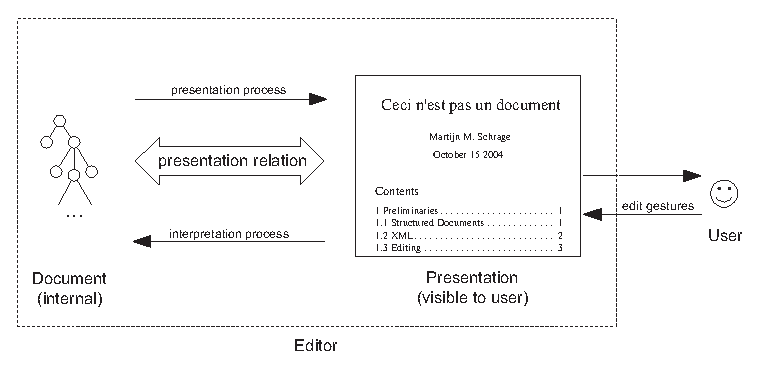
\epsfig{file=pics/eps/editor.eps, width=10cm}
\end{center}\caption{Schematic representation of an editor.}\label{editor} 
\end{center}
\end{small}
\end{figure}

% document and presentation
\vspace*{-1.2ex} Figure~\ref{editor} contains a schematic representation of an editor. The main data structures in the editor (also referred to as {\em levels}) are the internal {\em document} on the left that is not visible to the user and the user-visible {\em presentation} on the right. The document should not be confused with a file, which is a representation of the document that is stored on a file system. Furthermore, we also do not consider an XML source to be a document, but rather a textual presentation of the internal document.

\bc define levels \ec

A {\em presentation}, or {\em view}, is the only thing a user sees of the document. A presentation may be textual, graphical, or a combination of both. We focus on static presentations only. Hence, we do not explicitly consider presentations containing sounds or animations, unless presented statically (e.g.\ as a textual link to a sound or video file). In the presentation, the editor shows the focus of attention, or, for brevity, just {\em focus}, which is a shared name for the selection as well the cursor (which is an empty selection).  Several presentations of a single document may be shown simultaneously by the editor, each having its own focus. Finally, if a presentation closely mirrors the final physical appearance of the document when it is printed, it is referred to as a WYSIWYG presentation (What You See Is What You Get).

% what is presenting
The relation between a document and its presentation is denoted by the term {\em presentation relation}, or {\em presentation mapping}. If, according to the presentation relation, the presentation shown to the user is a presentation of the document, we say that the {\em presentation invariant} holds. Computing the presentation of a document is called the {\em presentation process}, whereas computing a document from a presentation is called the {\em interpretation process}. Together, the two processes implement the presentation relation and maintain the presentation invariant if either side of the relation changes.

% what is valid
A presentation is {\em valid} if there exists a document, which, when presented, yields that presentation. A presentation for which there is no corresponding document is invalid. An invalid presentation may result from an editing the presentation level. Note the difference with the term valid document, which denotes a document that is well typed.

\bc
When the presentation level is a presentation of the document, we refer to it as valid. This should not be confused with valid for XML documents which means type correct.
also in defs
\ec

% what is sheet
The presentation relation for an editor may be (partially) specified in a style sheet, or {\em presentation sheet}. A presentation sheet describes how elements of the document type are to be presented, and is a parameter of the presentation process. By modifying the sheet, a user may influence the appearance of the document without having to modify the editor itself. A presentation sheet can be regarded as a parameter to the interpretation process as well, since the interpretation depends on the presentation specified in the sheet. Examples of style-sheet formalisms are the Cascading Style Sheets (CSS)~\cite{css2} for HTML as well as XML, and the Extensible Stylesheet Language (XSL)~\cite{xsl10} for XML.

%what is the editing process
Generally speaking, editing consists of repeated interactive cycles of presenting and interpreting. The editor shows a presentation of the document together with the current focus to the user. The user then provides the editor with an {\em edit gesture}, such as a key press or a mouse movement, which is interpreted as an update on the document. The document is then re-presented and shown to the user. The process is repeated until the user quits the editor. Chapters~\ref{chap:informalSpec} and~\ref{chap:formalSpec} provide a more formal description of the editing process.

\head{Document-oriented versus presentation-oriented editing}

% doc-oriented vs pres-oriented 
Because edit gestures may be targeted either at the document or the presentation, we distinguish two kinds of editing:  {\em document-oriented} versus {\em presentation-oriented} editing.

% also say document editing/presentation editing?

On the one hand, we have {\em document-oriented editing}, which consists of edit operations (including navigation and selection) that are targeted at the structure of the document rather than at its presentation. Examples are swapping two chapters in a word processor, selecting an entire chapter, or navigating to a next section.

On the other hand, {\em presentation-oriented} editing consists of edit operations on the presentation, which do not necessarily make sense at the document level. If a presentation is textual,  presentation-oriented editing amounts to freely editing the text. As an example, take the mathematical expression  
$(1+2) \times (3+4)$. Deleting the middle part $(1+\framebox{$\,2) \times ($}\,3+4)$ yields $(1+3+4)$ and is a presentation-oriented edit operation that does not directly correspond to a logical operation on the document level. Another example is navigating downwards in a formatted paragraph of a word processor, since the concept of lines in a paragraph only exists at the presentation level. 

Section~\ref{sect:intrProcess} provides a more thorough discussion of both document- and presentation-oriented  editing. Furthermore, the section discusses editing at several other levels, which are introduced at the beginning of Chapter~\ref{chap:proxArch}.
%doc editing is usually also pres editing

\head{Different kinds of editors}

%what is structure editor
The term {\em structure editor} is used to make explicit that an editor has document-oriented editing functionality (also including navigation). We do not make a sharp distinction between plain-text editing and structure editing. Instead, we regard all editing as structure editing, but with a varying level of structure. A text editor can be seen as a structure editor with a very simple structure model: a string or a list of strings. Document-oriented and presentation-oriented editing coincide for a text editor.

%what is generic?
An editor is a {\em generic editor} if it is not specifically built for a single document type but can be used to edit a whole class of document types. A generic editor may be {\em instantiated} to yield an editor for a specific document type. Genericity can be achieved with a single generic editor that edits documents of arbitrary types, but also with an editor generator. An {\em editor generator} is an environment that generates an editor application based on descriptions of the document type and its presentation. Although a generator is not as versatile as a single generic editor, we view both as generic editors. 

%structure editor is not nec. generic
For brevity, we will often adopt the common practice that the term structure editor implies genericity as well. Still, structure editors that are not generic are quite common. A few examples are: equation editors, bookmark editors in web browsers, and file browsers. On the other hand, a generic editor is always a structure editor since it knows about the type of the document.


%??maybe introduce XML Editor here? and forward ref?

%who is the user of a generic editor?
In the context of generic editing, the term {\em user} is ambiguous. A user can either be an editor designer, who instantiates the generic editor for a specific domain, or a user who is editing a document. Unless explicitly stated otherwise, we use the term for the document-editing user.


\bc
When regarded as an editor, more sophisticated input fields that incorporate parsers, may be used. Furthermore, normal undo/redo functionality is possible, instead of the course grained OK/Cancel model, which only allows accepting or ignoring all changes at once.
\ec

\bc
% misschien niet zo'n interessante para
With such a broad view of editors, it is possible to regard every application, and even an entire operating system as an editor. In essence, all a computer user does is give edit gestures with the mouse and the keyboard in response to the presentation on the computer monitor. In reaction to the edit gestures, the internal state of the computer changes, giving rise to a new presentation. 

% en nog een
There is no fundamental problem with this view, but we do not adopt it because a definition that is too broad does not help in finding appropriate abstractions for a generic structure editor. Therefore, we do not explicitly consider all applications to be editors, but adopt the view that many applications contain editors.
\ec


Because it is difficult to give a precise definition of a generic structure editor and because such a definition might be restrictive, we will discuss a number of typical use cases to clarify what we mean by a generic structure editor. Section~\ref{sect:usecases} presents these use cases.





%								
\subsection{Advantages of generic structure editors}

An editor that knows about the structure of the edited document can offer interesting functionality. We list several potential advantages of generic structure editors. The first two advantages stem from the genericity of the editor, whereas the rest are mainly about the structural (document-oriented) abilities.

\begin{description}
\item[Uniform user interface/edit model.] Rather than a separate editor application for each type of document, a single generic editor can be used for a range of document types. Thus, instead of having to cope with several slightly different interfaces, a user only needs to deal with a single uniform interface and edit model.

\item[Integration of documents.] Besides offering editors for different types of documents, a structure editor also facilitates the integration of different types of documents into a single editor instantiation. Thus, it is relatively easy to build an editor for a specific document type, with advanced functionality for the different kinds of edit. Examples are a word-processing editor with spreadsheet functionality, or an editor for slide shows that has syntax coloring and type checking for program code appearing in the slides.

\item[Different Views on the Document.] A structure editor may provide a user with several editable views on the document. The views can show the document in a different order, or with a varying amount of detail. 

\item[Graphical Views.] A view may contain color and fonts in order to clarify document structure, but also use layout alignment, and graphical elements such as lines and boxes.

\item[Derived Information in the Presentation.] The editor can analyze the document during editing and display information computed from the document structure. Examples are the results of static analysis and type checking in source editors, but also chapter numbers or an automatically generated table of contents.

\item[Structural Edit Operations.] Certain edit operations, such as demoting a section with subsections to a subsection with subsubsections in a scientific article, are straightforward to specify at the structural level, but awkward at the presentation level.

\item[Structural Navigation.] Navigating over the document structure instead of its presentation can be very useful. In a source editor, when the focus is on an identifier, a user may easily navigate to its definition in the source. Furthermore, an outline view of the document can be shown in which a user can click to navigate to the corresponding position in the document.

\item[Integration with Other Tools.] A structure editor allows fine control over integration with other tools, such as spell checkers, program-transformation systems, and theorem provers. Furthermore, the editor may show the results coming from these tools at the appropriate position in the presentation, rather than as a list of messages with line numbers.


\end{description}

For document types with a textual presentation, such as program sources or XML documents, some of the advantages can be simulated with a text editor. Lexical analysis can be used on the edited text, and basic support for syntax coloring, auto-completion, and navigation can be provided. However, although simple and efficient, these solutions are  very basic and prone to errors, because, in general, much of the structure of a document cannot be recognized at a purely lexical level.

\bc
sometimes basic structural navigation.  Even though some of the document structure can be recognized at lexical level, in the general case, a full parse is needed. For example, when trying to specify a Haskell function definition as a line in which a '=' character is present, also lines containing strings or comments with '=' characters are identified as function definitions. In some cases the problems can be overcome, but in general this amounts to building a parser in a formalism that is too weak for that purpose. Therefore, we will not consider text editors in this overview of editors.
%*********************************
\ec

% maybe say we  explain why this is the case
% maybe say we will change it? or put that in outline?

% pan article




%								
\subsection{Classes of structure editors} \label{sect:classes}

Three classes of structure editors are distinguished in the literature: {\em syntax-directed}, {\em syntax-recognizing}, and {\em hybrid} editors. Syntax-directed editors mainly support edit operations targeted at the document structure, whereas syntax-recognizing editors support edit operations on the presentation of the document. A hybrid editor combines syntax-directed with syntax-recognizing features, but the term is not used consistently. 
%To avoid confusion, we will refrain from using the term hybrid, except in the brief discussion below.

\head{Syntax-directed editors} 
% mention that structure editing is often source editing.

The first structure editors that were developed are the {\em syntax-directed}, or {\em pure}, structure editors~\cite{reps84synGen,Bahlke86PSG,magnusson90orm}.

Early syntax-directed editors show a textual presentation of the document (usually a program source) but exclusively offer edit operations targeted at the internal document structure, and not at the textual presentation. The original idea behind this was that if structural edit operations are available, a user would not need the textual edit operations anymore. Further, presentation-oriented edit operations would interfere with the user's structural model of the document and introduce errors. Hence they were prohibited altogether. Most editors for XML (see also Section~\ref{sect:xmlEditors}), as well as editors for preferences panes, can be regarded as syntax-directed editors.




\begin{figure}
\begin{small}
\begin{center}
\begin{center}
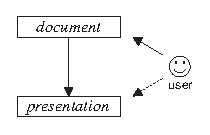
\epsfig{file=pics/eps/SynDirEditor.eps, width=3.5cm}
\end{center}\caption{A syntax-directed editor.}\label{synDirEdit} 
\end{center}
\end{small}
\end{figure}


Figure~\ref{synDirEdit} shows a schematic representation of a syntax-directed editor. The editor works by computing a presentation of the internal document structure, which is shown to the user together with a current focus of attention. The user provides an intended edit operation (edit gesture) on the document structure, from which a document update is computed. After the document is updated, a new presentation is computed, which is shown to the user.

If the editor supports clicking in the presentation to set the focus, the editor also needs to keep track of the origin in the document for each position in the presentation.

In the figure, the line between the user and the presentation is dotted because syntax-directed editors do not support edit operations on the presentation very well. Because the presentation is derived from the document, the editor needs to interpret the intended edit operation on the presentation as an edit operation on the document, which is difficult if the edit operation is not a logical operation on the document level.

A major problem with syntax-directed editors is the restrictiveness of the edit model (e.g.~\cite{vanter94practical,rubinNeal87design}). New structures are easy to create, but not as easy to modify. For example, if a user wishes to change a while statement to an if statement, simply typing over the keyword is typically not supported. 
\finallongpage

Many later syntax-directed editors offer a form of presentation-oriented editing by providing a freely editable textual presentation of (part of) the document, and applying a parser to the edited text. Some publications~\cite{teitelbaum81progSynth, minor90editing} refer to such editors as hybrid, but, as we will explain below, we still regard these editors as syntax-directed editors. 

Unless the two forms of editing are completely integrated, the textual presentation forces a user to work in a different mode of editing, which is referred to as {\em mode switching}. Mode switching does not solve the problem of restrictiveness adequately. Often, a separate window showing a text-only presentation is opened and before the mode can be switched back, the edited text has to be valid. Furthermore, separate modes require a user to be constantly aware of the current mode of the editor. The resulting increased cognitive burden has been shown to be a source of errors~\cite{sellen90modes}.

% mention problems?
\head{Syntax-recognizing editors} 

At the other end of the spectrum are the {\em syntax-recognizing} structure editors~\cite{budinsky85sre, ballance92pan}. A syntax-recognizing editor keeps track of the textual presentation of the document. The user can freely edit the text, and the editor tries to recognize the document structure by means of a parser. Once the text has been (partially) recognized, structural information (e.g.\ syntax-coloring or type information), navigation, and, in some editors, edit operations are available.

\begin{figure}
\begin{small}
\begin{center}
\begin{center}
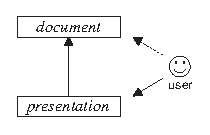
\epsfig{file=pics/eps/SynRecEditor.eps, width=3.5cm}
\end{center}\caption{A syntax-recognizing editor.}\label{synRecEdit} 
\end{center}
\end{small}
\end{figure}

Figure~\ref{synRecEdit} schematically shows a syntax-recognizing editor. The user's edit operations are targeted at the presentation, which can be edited freely. The document is derived by parsing (interpreting) the presentation; hence the reversed direction of the arrow, compared to Figure~\ref{synDirEdit}.

For each element in the document structure, the editor needs to keep track of what parts of the presentation it corresponds to, in order to show structural information in the presentation, as well as support structural navigation. When a document structure has been recognized, the presentation may show additional information using font and color changes, context-sensitive menus, tooltips, etc.
\finallongpage

Similar to the syntax-directed editor, the picture of the syntax-recognizing editor in Figure~\ref{synRecEdit} also contains a dotted arrow. In this case, because the document is derived from the presentation, structural edit operations on the document are difficult to support. A document-oriented edit operation has to be mapped onto an update on the presentation, in such a way that parsing the updated presentation returns the intended updated document. Presentation information that is not stored in the document tree, such as whitespace and comments, has to be related to the document tree in some way, in order to be put in the right place after a structural edit operation.

The main problem with syntax-recognizing editors lies in their limited applicability. Because the presentation needs to contain enough information to derive the document, interesting presentations that only show part of the document are hard to support. Furthermore, graphical presentations, as well as presentations containing computed values and structures, do not fit the model, as these are difficult to parse. As a result, syntax-recognizing editors are mainly limited to text-oriented applications, such as program-source editors.

% mention: good for program editing?
\head{Hybrid editors} 


A {\em hybrid} editor supports structural as well as presentation-oriented edit operations. Figure~\ref{hybridEditor} shows a hybrid editor. Because both levels can be edited, there are no dotted arrows in the figure. However, in order to offer this edit functionality, the editor must realize both the presentation and interpretation mappings. Hence the double arrow between the document and the presentation. 

In some publications (e.g.~\cite{teitelbaum81progSynth, minor90editing}), the term hybrid is used to refer to syntax-directed structure editors that have a limited form of syntax-recognizing functionality. As a consequence, most syntax-directed editors would qualify as hybrid editors, because most editors support some form of text parsing.

In contrast, other publications (e.g.~\cite{ballance92pan, koorn92gse}) advocate that the term hybrid should be reserved for editors that support full textual editing of the document, as well as limited syntax-directed functionality, even if structural modifications on the document are not supported. According to this view, almost all syntax-recognizing editors would classify as hybrid editors, since most of these editors support a form of structural navigation.

Because of the confusion, and because most editors tend to be either primarily syntax-directed or syntax-recognizing, we will often use those terms, instead of the term hybrid.


\section{Proxima} \label{sect:introProxima}

\begin{figure}
\begin{minipage}[b]{.47\textwidth}
    \begin{center}   
~~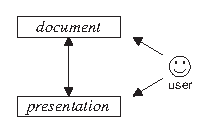
\epsfig{file=pics/eps/HybridEditor.eps, width=3.7cm}
\vspace{56.4pt}
      \caption{A hybrid editor.}\label{hybridEditor} 
    \end{center}
  \end{minipage}
\hfill
\begin{minipage}[b]{.47\textwidth}
    \begin{center}  
\hspace*{0.5cm}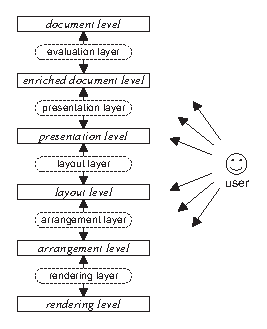
\epsfig{file=pics/eps/ProximaEditorLayers.eps, width=4.8cm}
%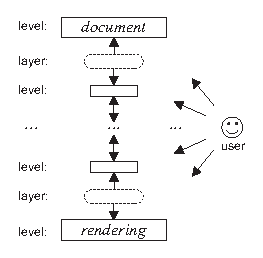
\epsfig{file=pics/eps/ProximaEditor.eps, width=4.7cm}
      \caption{Proxima.}\label{proximaEditor} 
    \end{center}
  \end{minipage}
\end{figure}


The subject of this thesis is the design of the presentation-oriented structure editor Proxima. Proxima is suitable for a wide range of applications, including word-processors and source editors, but also mathematical-equation editors and spreadsheets. An important aspect of Proxima is that the editor fully supports presentation-oriented as well as document-oriented editing. Thus, the editor classifies as a hybrid structure editor.

The implementation of the bidirectional mappings between the document and the presentation is facilitated by a layered architecture. The computation of the presentation is broken up in several stages, and each intermediate value in this computation corresponds to a {\em data level} (or just {\em level}). The interpretation process has the same intermediate values. Between two levels, there is a {\em layer}, which is a component that takes care of mapping values at one level onto values at another level, and thus implements a single stage of the presentation and interpretation processes. 

\bc
Figure~\ref{proximaEditor} sketches the levels and layers of Proxima. Because the name {\em presentation} is reserved for one of the intermediate levels, the lowest level is referred to, more appropriately, as the {\em rendering} level. The figure shows multiple edit arrows coming from the user, because edit operations may be targeted at intermediate stages as well. A more detailed discussion of the levels and layers is provided in Chapter~\ref{chap:proxArch}. 
\note{mention sheets?} 
\ec

The first step of the presentation process is that the {\em document} is enriched with computed values and structures, by the evaluator. The resulting {\em enriched document} is mapped onto a logical {\em presentation} in which positions and sizes are specified relatively. The layout layer adds whitespace that is not stored in the document to the presentation, yielding the {\em layout} level. The layout level is mapped onto an {\em arrangement} level, which contains absolute positions and sizes. And finally, the renderer maps the arrangement onto a {\em rendering}, which is made visible to the user. A more detailed discussion of the presentation and interpretation processes is provided in Chapter~\ref{chap:proxArch}.


Figure~\ref{proximaEditor} shows the levels and layers of Proxima. Because the name {\em presentation} is reserved for one of the intermediate levels, the lowest level is referred to, more appropriately, as the {\em rendering} level. The figure shows multiple edit arrows coming from the user, because edit operations may be targeted at intermediate levels as well.

% by breaking up the interpretation problem
The layered architecture makes it possible to combine presentation-oriented editing with a powerful document-presentation mechanism that includes support for derived values and structures. A platform-independent Haskell prototype of Proxima has been implemented, and experiments with instantiated editors have yielded promising results.

%\begin{figure}
%\begin{small}
%\begin{center}
%\begin{center}
%\begin{small}
%\noindent
%\xymatrix@=0.4cm{
%   \dataa{$Document$}  \ar[dd]   &     \\
%                                            & User  \ar[ld]\ar[lu] \\
% \dataa{$Presentation$} \ar[uu] &   \\
%}
%\xymatrix@=0.4cm{
%   \dataa{$Document (Level_0)$}  \ar[d]   &     \\
%   \dataa{$Level_1$}  \ar[d]\ar[u]   &     \\
%   \dots                                           & User  \ar[ldd]\ar[ld]\ar[lu]\ar[luu] \\
% \dataa{$Level_{n-1}$} \ar[u] \ar[d] &   \\
% \dataa{$Presentation (Level_n)$} \ar[u] &   \\
%}
%\end{small}
%\end{center}\caption{Proxima (draft)}\label{synRecEdit} 
%\end{center}
%\end{small}
%\end{figure}

 
% what about backward mapping, no ES needed? Probably won't know this until some more
% research is done on mappings


\section{Terminology}\label{sect:terminology}

We give a brief summary of the terms that were introduced in the previous sections.

\begin{description}
\item[Editor:] Application for creating and modifying documents. In this thesis, the term also used to refer to structure editors and generic editors (or generic structure editors).
\item[Document:] Internal data structure that represents the information that is edited.
\item[Presentation:] Denotes a visible representation of the document (also called a {\em View}), as well as one of the intermediate levels of the presentation process. 
\item[Presentation mapping/relation:] The relation between the document and its presentation.
\item[Presentation-oriented editing:] Edit operation targeted at the presentation:\\ e.g.\ deleting ``\;$+$\;'' from ``$1+2$'', yielding ``$12$''.
\item[Document-oriented editing/Structure editing:] Edit operation targeted at the document: e.g.\ swapping two sections in an article.
\item[Presentation sheet:] Parameter to the presentation/interpretation process. 
\item[Presentation process:] Process of computing the presentation of a document.
\item[Interpretation process:] Process of computing a document from a presentation.
\item[Level:] Intermediate value of the presentation/interpretation process, including the document and the presentation.
\item[Layer:] Component that realizes the presentation and interpretation between two levels.
\item[Structure editor:] An editor that has knowledge of the structure of the edited document. Usually assumed to be a {\em generic editor} as well.
\item[Generic editor:] A structure editor that is suitable to edit documents of different types.
\item[Syntax-directed editor:] An editor that primarily supports document-oriented editing.
\item[Syntax-recognizing editor:] An editor that primarily supports presentation-oriented editing.
\item[Valid document:] A well-typed document, mainly used in the context of XML.
\item[Valid presentation:] A presentation that is the result of presenting some document.
\item[Focus:] Shared name for cursor and selection.
\end{description} 

%\section{Why Proxima}
%
%(Will be added when all chapters are more or less finished)

%Why proxima
\bc
complex, but:
new stuff:

-extra state
-also editing on all? levels

Document standard XML getting popular, need editors.

interactive transformations, proof editors, rewrite systems
structural data complex presentations: math
programs with types and structural edit ops: IDEs

Proxima not about changing the world: struct editors, views.  editors have illogical/inconsistent features. Easiest to start all over with new model, however will frustrate users. Better to have a model that allow to express the familiar edit models. and merge them seamlessly.
\ec


\section{Outline of the thesis}\label{sect:overview}

The remainder of this thesis has the following structure:

%As mentioned, users regard structure editors as being either overly restrictive, and/or not powerful enough.
Chapter~\ref{chap:requirements} explores applications of generic structure editing by providing five use cases of real-world editors. With these use cases in mind, we formulate a number of functional requirements that in our view are important for a flexible non-restrictive structure editor. We evaluate a number of existing editors according to the requirements, and conclude with an overview of how the Proxima editor is designed to meet the requirements and be able handle all use cases.

The layered architecture of Proxima is introduced in Chapter~\ref{chap:proxArch}.  The chapter discusses the various data levels, as well as the layers that maintain the mappings between the levels. The discussion is illustrated with examples of the presentation and interpretation processes.

In chapters~\ref{chap:informalSpec} and~\ref{chap:formalSpec}, we develop a specification of the Proxima editor. Chapter~\ref{chap:informalSpec} serves as an introduction to the specification and introduces our model of the edit process, as well as the concepts of extra state and duplicates in the presentation. In  Chapter~\ref{chap:formalSpec}, we start by specifying a simple editor, to which extra state and multiple layers are added in subsequent sections. The chapter ends with an informal discussion on how to handle presentations that contain duplicates.

In Chapter~\ref{chap:presenting}, we discuss the {\Xprez} presentation formalism of the Proxima. {\Xprez} is a declarative presentation language, suited for specifying a wide range of presentations. We state a number of requirements for a presentation language for structured documents, and provide an informal overview of {\Xprez}, using a series of examples.

A prototype that offers much of the functionality discussed in this thesis has been implemented in the functional language Haskell. Chapter~\ref{chap:prototype} discusses the prototype as well as a number of editors that have been instantiated. The chapter also explains which components need to be provided to instantiate an editor.

Finally, Chapter~\ref{chap:conclusions} presents the conclusions and gives an overview of future research.


\bc
* mention here or in chapter proxArch? (or at all?)
Bootstrapping problem, descr. of levels layers and edit model. second is easier to give with in a formal story. however, design reasons for first are hard to comprehend without idea. So first informal arch and edit model and later the formal stuff

\ec	% 1
\setcounter{chapter}{1} \chapter{Requirements for a structure editor} \label{chap:requirements}

%{\em *** Version: \today~ ***}


\bc

TODO: change wordprocessor screenshot to actual thesis chapter text

Whitespace in use cases
Layout/captions of screenshots

Add Eclipse!





Mention OpenDoc, Views? Not really structure editors.

mention that instead of preventing syntax errors, continuous parsing with in-place error 
info is a good model as well?

incrementality  has been removed from this chapter
Also, we have not paid much attention to incrementality. The layered architecture of Proxima allows incrementality issues to be dealt with by individual layers. 

With current computer speeds, parsers are so fast that incremental parsing has become %less of an issue. We expect that a rather coarse model for incrementality in the %presentation will be sufficient for creating fast editors.
\ec

\bc
Editing is concerned with the creation and maintenance of documents.  
Most documents have some form of structure. 

In this chapter, we give a rather informal definition of editing (editor?**), and look at why no str eds. From a number of use cases, we state a number of requirements that are important in the design of a generic structure editor. Other structure editors are evaluated on these requirements, and . We end with a discussion why no structure editor has yet .  give fun. req. and evaluate related work according to them. End with a discussion why no editor meets all requirements, and how Proxima will.
\ec

In this chapter, we present five use cases of possible applications for a generic structure editor. The use cases will shed more light on the definition of the term editor from the previous chapter, as well as provide standard examples to explain and define edit behavior in the coming chapters. A design requirement of Proxima is that the editor is able to handle all five use cases. 

Section~\ref{sect:usecases} presents the five use cases, from which we formulate a set of functional requirements for a flexible non-restrictive structure editor, in Section~\ref{sect:reqs}. Existing editors are evaluated according to these requirements in sections~\ref{sect:overview} and~\ref{sect:discussion}, showing why none of these editors can handle all use cases. Finally, in Section~\ref{sect:proxEditor} we discuss how the Proxima editor meets the requirements and thus will be able to implement all of the use cases.

\section{Use cases} \label{sect:usecases}

Some of the five example editors, presented in this section, are well-known applications of structure editors. However, a few more exotic applications have been included as well. None of the current generic structure editors can handle all five use cases.

It is important to note that although the use cases are discussed as separate applications, aspects of them can be combined in a single editor instance.


%								
\subsection{A source editor for Haskell}  \label{sect:sourceeditor} 

As an example of a program-source editor, we take an editor for the functional programming language Haskell~\cite{peytonJones03haskell}. The editor supports an extended form of syntax highlighting, in-place display of syntactic and semantic errors, and a range of language-specific edit operations. 

There exists evidence showing that syntax highlighting makes programs more readable~\cite{baecker88readability, omanCook90typography}. Our editor also supports highlighting at a semantic rather than syntactic level. Hence, unlike most text editors, the editor can use different display styles for language constructs that are hard to recognize purely syntactically. The type declarations in the next screenshot\note{The screenshots in this chapter are still drafts because they may be replaced by actual Proxima screenshots.} are an example of such a construct. Although syntactically identical, identifiers in type expressions are colored differently from identifiers in ordinary expressions.

%mention module handling etc.?
 
\screenshot{$\langle$Haskell listing with syntax coloring and type information$\rangle$}{The Haskell source editor}
%(also type decls) type info in layered menu? (see text below) 

Haskell is a particularly interesting language for a source editor because, due to Haskell's rich type system, information about types is very useful during programming. Haskell programmers often experience that once type errors have been removed, a function is correct. Therefore, an environment that supports in-place display of type errors, as well as easy access to type information of variables in scope, will help rapid program development. 

The screenshot shows the type of the expression in focus, together with a list of variables in scope. Selection in the menu causes a jump to the definition of the identifier. Because many identifiers may be in scope, the menu is layered according to scope level. 

%

\head{Automatic layout}

Some structure editors use an automatic layout scheme while editing program sources. The user then does not need to worry about layout issues, such as the alignment of parameters in functions with multiple clauses. However, for a Haskell editor this situation is not optimal because Haskell programs mainly consist of expressions, which are hard to layout automatically. Therefore, rather than having automatic layout be continuously performed on the entire source, a user may request the editor to automatically lay out a selected part of the program. The specification of the layout of the program is part of a presentation sheet and may be adapted by the user. Of course, if desired, it is also possible to turn on continuous automatic layout.


\newcommand{\editScreenshot}[4]{%
%
\noindent
\begin{center}
\begin{picture}(350,135)(0,0)
\begin{scriptsize}
\put(0,30){ \framebox(160,105){#1}}
\put(180,30){ \framebox(160,105){#2}}
\end{scriptsize}
\put(165,80){ $\Rightarrow$}
\put(0,0) { \makebox(160,30){#3}}
\put(180,0) { \makebox(160,30){#4}}
\end{picture}
\end{center}
}

\newcommand{\editScreenshotTrns}[3]{%
%
\noindent
\begin{center}
\begin{picture}(350,130)(0,0)
\begin{scriptsize}
\put(0,30){ \framebox(160,105){#1}}
\put(180,30){ \framebox(160,105){#2}}
\end{scriptsize}
\put(165,80){ $\Rightarrow$}
\put(96,0) { \makebox(150,30){#3}}
\end{picture}
\end{center}
}

\editScreenshotTrns{
\ttfamily 
\begin{tabular}[t]{@{}l@{}}
\begin{tabular}[t]{@{}l@{}}
tails~::~[a]~->~[[a]]\\
tails~[]~=~[[]]\\
tails~xxs@(\_:xs)~=~xxs:tails~xs\\
\end{tabular}
\\
\begin{tabular}[t]{|@{}l@{}|}
\hline
prefix~::~(Eq~a)~=>~[a]~->~[a]~->~Bool\\
prefix~[]~\_~=~True\\
prefix~\_~~[]~=~~False\\
prefix~(x:xs)~(y:ys)~=~if~x~==~y~then\\
~~~~~~~~~~~~~prefix~xs~ys~else~False\\
\hline
\end{tabular}\\
\\
\begin{tabular}[t]{@{}l@{}}
suffix~::~(Eq~a)~=>~[a]~->~[a]~->~Bool\\
suffix~x~y~=~reverse~x~`prefix`~~reverse~y\\
\\
\end{tabular}
\end{tabular}
\rmfamily
}
{
\ttfamily 
\begin{scriptsize}
\begin{tabular}[t]{@{}l@{}}
\begin{tabular}[t]{@{}l@{}}
tails~::~[a]~->~[[a]]\\
tails~[]~=~[[]]\\
tails~xxs@(\_:xs)~=~xxs:tails~xs\\
\end{tabular}
\\
\begin{tabular}[t]{|@{}l@{}|}
\hline
prefix~::~(Eq~a)~=>~[a]~->~[a]~->~Bool\\
prefix~[]~~~~~\_~~~~~~=~True\\
prefix~\_~~~~~~[]~~~~~=~False\\
prefix~(x:xs)~(y:ys)~=~if~x~==~y\\
~~~~~~~~~~~~~~~~~~~~~~~then~prefix~xs~ys\\
~~~~~~~~~~~~~~~~~~~~~~~else~False\\
\hline
\end{tabular}\\
\\
\begin{tabular}[t]{@{}l@{}}
suffix~::~(Eq~a)~=>~[a]~->~[a]~->~Bool\\
suffix~x~y~=~reverse~x~`prefix`~~reverse~y\\
\end{tabular}
\end{tabular}
\end{scriptsize}
\rmfamily
}{apply layout}

The screenshot shows the automatic-layout operation applied to the selected function {\tt prefix}. The layed-out function on the right-hand side is still freely editable, including its whitespace.
% comment handling?

\head{Structural edit operations}

Because a program construct is represented by a contiguous area in the presentation, moving a program construct can usually be done in a straightforward way by moving its presentation. However, this is not always the case. Consider for example the following let expression:

\smallScreenshot{let \framebox{x=1}; y=2 in x+y}{after select}

The let expression consists of a list of declarations that are separated by semicolons and whitespace. Contrary to, for example, the language Java, the semicolon in Haskell acts as a separator, and not as a terminator. Unlike a terminator, which can be regarded as part of the presentation of a declaration, a separator belongs to the presentation of the list of declarations. As a result, semicolons may cause problems when declarations are moved.

Consider moving the first declaration (\verb|x = 1|) to the end of the let expression. When the declaration is cut, the semicolon behind it must be deleted, and when the declaration is pasted at the end, a semicolon together with appropriate whitespace must be added. Similar issues apply to all list structures that are presented using separators, such as Haskell lists \verb|[1, 2, 3]|, tuples \verb|(1,2,3)|, or monadic \verb|do| expressions \verb|do {a <- getChar ; putStr [a]}|.

If the structure of the edited list is taken into account, cut-and-paste on lists with separators can be handled elegantly. When the first declaration is selected, the editor recognizes it as an element of the let expression's declaration list, and when it is cut, the semicolon next to it disappears:

\editScreenshot{let y=2 in \underline{x}+y}{let y=2; \framebox{x=1} in x+y}{after cut}{after paste}

When the declaration is pasted, a semicolon is automatically placed in front of it. The whitespace from the semicolon is copied from the whitespace of the other semicolons in the presentation (or may come from a pretty-printing algorithm). If the list has an irregular layout (e.g.\ \verb|[1,  2,    3, 4]|), the layout after the paste operation may not be what is expected. However, since list structures are usually layed out in a regular way, this need not be a problem.

\head{Rename within scope}

A second example of an edit operation that takes the document structure into account is a rename operation on an identifier. In a regular text editor, occurrences of the identifier name need to be changed using search and replace. However, automatic search and replace does not always lead to the desired result because the identifier may be redeclared in inner scopes, or the identifier name may appear in a string.

\editScreenshotTrns{f \framebox{a} b = a + let a = 10 in a }{f \framebox{x} b = x + let a = 10 in a }{rename variable}

% a function is a better example
The rename operation takes account of the scoping rules of Haskell, and only changes the appearances that lie in scope of the updated identifier. If the new name is captured by an inner declaration, or if it shadows an identifier that is already declared, a warning is issued.

The rename operation is an example of a {\em refactoring} operation: a source-to-source program transformation that leaves  the functionality of the program intact. The designers of the Haskell Refactorer~\cite{reinke03refactoring} identify a number of such transformations.

\head{Hide function definitions/folding}

Function definitions in the source presentation may be collapsed, leaving only one left-hand side and the (possibly inferred) type declaration. This operation is often referred to as folding.

\editScreenshotTrns{
\begin{tabular}[t]{l}
%{\tt yA (LineA \_ x y x' y' \_ \_)~~~= y}\\
%{\tt yA (PolyA \_ x y w h \_ \_ \_ \_)~= y}\\
%{\tt yA (RowA \_ x y w h \_ \_)~~~~~~= y}\\
{\tt yA (ColA \_ x y w h \_ \_)~~~~~~= y}\\
{\tt yA (OverlayA \_ x y w h \_ \_)~~= y}\\
\\
\begin{tabular}[t]{@{}l@{}l}
{\tt widthA :: Arrangement $\rightarrow$ Int}\\
{\tt widthA (StringA \_ x y w h \_ \_ \_ \_)} &\p{ = w}\\
{\tt widthA (ImageA \_ x y w h \_ \_ \_ \_)} &\p{  = w}\\
{\tt widthA (PolyA \_ x y w h \_ \_ \_ \_)} & \p{ = w}\\
{\tt widthA (RowA \_ x y w h \_ \_)} & \p{ = w}\\
{\tt widthA (ColA \_ x y w h \_ \_)} & \p{ = w}\\
{\tt widthA (OverlayA \_ x y w h \_ \_)} & \p{ = w}\\
\end{tabular}
\\
\\
{\tt heightA :: Arrangement $\rightarrow$ Int}\\
{\tt heightA (StringA \_ x y w h \_ \_ \_ \_)~= h}\\
\end{tabular}
}{
\begin{tabular}[t]{l}
%{\tt yA (LineA \_ x y x' y' \_ \_)~~~= y}\\
%{\tt yA (PolyA \_ x y w h \_ \_ \_ \_)~= y}\\
%{\tt yA (RowA \_ x y w h \_ \_)~~~~~~= y}\\
{\tt yA (ColA \_ x y w h \_ \_)~~~~~~= y}\\
{\tt yA (OverlayA \_ x y w h \_ \_)~~= y}\\
\\
 {\tt widthA :: Arrangement $\rightarrow$ Int}\\
{\tt widthA = \framebox{\rule{0cm}{1.5ex}\dots}}\\
\\
\begin{tabular}[t]{@{}l@{}l}
{\tt heightA :: Arrangement $\rightarrow$ Int}\\
{\tt heightA (StringA \_ x y w h \_ \_ \_ \_)}&\p{ = h}\\
{\tt heightA (ImageA \_ x y w h \_ \_ \_ \_)}&\p{ = h}\\
%{\tt heightA (LineA \_ x y x' y' \_ \_)}&\p{ = y'-y}\\
{\tt heightA (PolyA \_ x y w h \_ \_ \_ \_)}&\p{ = h}\\
{\tt heightA (RowA \_ x y w h \_ \_)}&\p{ = h}\\
{\tt heightA (ColA \_ x y w h \_ \_)}&\p{ = h}\\
{\tt heightA (OverlayA \_ x y w h \_ \_)}&\p{ = h}
\end{tabular}
\end{tabular}
}{hide function definition}

The two functions \verb|widthA| and \verb|heightA| have a large number of clauses. Hiding these clauses may improve the readability of the source. After applying the {\em hide function body} edit operation to the function \verb|widthA|,  only one clause remains with a collapsed right-hand side ({\tt \framebox{\rule{0cm}{1.5ex}\dots}}). The function is expanded again by clicking on the dots. A collapsed function may be renamed, deleted, or structurally moved around in the source. Editing the whitespace around the `\verb|=|' sign would be ambiguous because of the hidden parameters names and the fact that a single collapsed function typically represents several clauses. Hence, editing this whitespace is not allowed.

\head{Requirements} % haskell editor

The source editor generates a number of requirements, an important one being the possibility of freely editing the textual program source, including the layout. At the same time, it must be possible to let the layout be computed automatically as well. Furthermore, a formalism for specifying computations over the document is required for performing static analysis and type checking.

Freely editing the program source is not always regarded a requirement for a structure editor. Purists argue that text editing may introduce syntactic errors, and that it is not necessary for programming (e.g.~\cite{teitelbaum81progSynth, magnusson90orm}). However, no clear consensus has been reached on the subject (e.g.~\cite{abandonText82waters} and reactions \cite{shani83notAbandon, responseToWaters83notkin}, and \cite{vanter94practical}) and nowadays most syntax-directed editors support some form of free text editing. Furthermore, because up to now no pure syntax-directed editor has ever become popular with programmers, we believe that free textual editing is an essential requirement for a program-source editor.


%																
\subsection{A word processor} \label{sect:wordprocessor} 

\nonote{Text in screenshots is no longer correct}

This section describes a WYSIWYG document editor with a user interface similar to word-processing applications such as Microsoft Word, but with a document model similar to the XML/SGML DocBook standard~\cite{walsh02docbook} and an output quality similar to \TeX~\cite{knuth84tex}. Examples of editors with similar functionality are TeXmacs\cite{texmacs} and Lyx~\cite{lyx}, but neither system is generic.

\screenshot{$\langle$Word-processor document with table of contents, citations, etc.$\rangle$}{The word processor}

The document model consists of chapters, sections and subsections. The editor supports free editing in the WYSIWYG presentation with optimal line breaking, a derived table of contents, and an automatic bibliography. Cross-references, such as citations or references to figures, can be clicked to bring the referred part of the document into focus.

\head{Structural view on the document}

Although Microsoft Word is one of the most popular word-processing tools in the world, an often-heard complaint concerns its confusing document model. Sometimes edit operations are not allowed because of underlying document structure, but it is not obvious why this is the case. Furthermore, the reason why a document fragment looks the way it does is not always clear. The user may have set specific style attributes for a particular fragment, or the style may originate from the document's presentation rules. A more structural view on the document, such as WordPerfect's ``underwater'' screen, can help to clarify the situation, but is not supported by Microsoft Word. Such a structural view is easily defined in a structure editor:

\editScreenshotTrns{
\begin{tabular}{l}
\rmfamily
normal text {\em {\bf \em italic and bold} just italic} normal\\
text again {\bf \em plus a warning}.\\
\end{tabular}
}{
\begin{tabular}{l}
normal text $\langle$e$\rangle$$\langle$b$\rangle${\em {\bf \em italic and bold}}$\langle$/b$\rangle$ {\em just}\\
{\em italic}$\langle$/e$\rangle$ normal text again $\langle$Warning$\rangle${\bf \em plus a} \\
{\bf \em warning}$\langle$/Warning$\rangle$.\\
\end{tabular}
}{switch to structural presentation}

The two screenshots show two presentations of the same document fragment. The left-hand presentation is the regular WYSIWYG presentation, whereas the right-hand one is a more structural presentation that shows the markup tags. The example document also contains a fictitious \verb|<Warning>| element that is presented in a bold and italic style. Only in the structural presentation can the warning be distinguished from text that has been explicitly formatted as bold and italic.

The structural view is also helpful for positioning the focus. For example, in the left-hand presentation, the start of the first piece of italic text just before the bold part coincides with the start of the bold part; therefore inserting text that is italic but not bold is rather tricky. In the right-hand presentation the positions do not coincide and text that is only italic as well as text that is italic and bold can be inserted without a problem. In order for the structural views to be helpful, the editor supports easy switching between views while preserving the current focus.

%Handles to invisible stuff, attributes?

\head{Structural edit operations}

Edit operations that rearrange the document structure, such as promoting a subsection to section, are awkward to perform on a textually represented document, such as a \TeX\ source. All tags or \TeX\ commands that specify the subsection and its descendants need to be changed. This is a rather specific search/replace operation on only part of the document source, which is a hassle to automate.

A structure editor may be of some help here, because the structural similarities between sections and subsections are known to the editor and can be used to define edit operations for restructuring the document.

\editScreenshotTrns{
\begin{tabular}[t]{l}
1~~Editing~structured~documents\\
~~1.1~~Classes of structure editors\\
~~1.2~~Advantages of structure editors\\
~\,\fbox{1.3~~Use cases}\\
~~~~1.3.1~~A source editor for Haskell\\
2~~Functional requirements
\end{tabular}
}{ 
\begin{tabular}[t]{l}
~1~~Editing~structured~documents\\
~~~1.1~~Classes of structure editors\\
~~~1.2~~Advantages of structure editors\\
\,\fbox{2~~Use cases}\\
~~~2.1~~A source editor for Haskell\\
~3~~Functional requirements
\end{tabular}
}{change to section}
 
The screenshot shows the effect of the structural edit operation {\em change to section}. If the containing section ``Editing structured documents'' had had any subsections following the promoted subsection, these could have become subsections of the new ``Use cases'' section. However, different behavior for such sections may be specified by the user in a preferences window for the command.

An operation that changes the level of a section or subsection is rather complex because it involves splitting and changing elements. Moreover, there are special cases to consider. For example, if a subsubsection is the deepest possible structural level, a warning needs to be issued when a section containing a subsubsection is demoted to subsection. Therefore, such an operation needs to be specified explicitly by the editor designer or user. Other document operations, however, such as splitting and joining elements of a list, may be derived automatically.
% show transf. spec. language?

% link to outline ed, and support moving of structures?

\head{Editing a section title in the table of contents}

The word processor has support for the specification of a generated table of contents. From an entry in the table, a user can jump to the corresponding position in the document presentation. The presentation of the table of contents itself can be customized to match the style of the rest of the presentation. When the document is edited, the table of contents is updated accordingly. Moreover, editing an entry in the table of contents causes an update to the title of the corresponding chapter or section.

\editScreenshotTrns{
\begin{tiny}
\begin{tabular}[t]{p{5.2cm}}
{\small Contents}\\
\vspace{0.001cm}
~~~1~~Editing~structured~documents\\
~~~2~~\framebox{\!U\!}se cases\\
~~~\dots\\
\vspace{0.005cm}
{\small 1~~Editing~structured~documents}\\
\vspace{0.001cm}
While the term {\em editor} is usually only associated with text editors such as Emacs~\cite{stallman81emacs}, we will use \\
% it in a much broader sense. We regard \dots\\ 
\dots \\
\vspace{0.005cm}
{\small 2~~Use cases}\\
\vspace{0.001cm}
In this section we present five example applications of a generic structure editor. Some of these \\
% cases are well-known \dots\\
\dots
\end{tabular}
\end{tiny}
}{
\begin{tiny}
\begin{tabular}[t]{p{5.2cm}}
{\small Contents}\\
\vspace{0.001cm}
~~~1~~Editing\\
~~~2~~The use cases\\
~~~\dots\\
\vspace{0.005cm}
{\small 1~~Editing~structured~documents}\\
\vspace{0.001cm}
While the term {\em editor} is usually only associated with text editors such as Emacs~\cite{stallman81emacs}, we will use \\
%it in a much broader sense. We regard \dots\\ 
\dots \\
\vspace{0.005cm}
{\small 2~~The use cases}\\
\vspace{0.001cm}
In this section we present five example applications of a generic structure editor. Some of these \\
%cases are well-known \dots\\
\dots
\end{tabular}
\end{tiny}
}{enter: ``\p{The\spc u}''}
% In final picture maybe use Lambert's idea instead of dots? (3 different blocks, each with zigzag ends)

The screenshot shows a document with a table of contents. The dots (\dots) are not part of the actual screenshot, but have been added to show the table of contents together with the section headings. The second entry in the table of contents is edited by entering the text ``The u'' over the selected letter 'U' at the beginning of the title. The result is that both the entry in the table of contents as well as the title in the presentation of the section itself change to ``The use cases''.

\head{Moving a section in the table of contents}

Besides textual edit operations, it is also possible to perform structural edit operations on derived structures. The screenshot shows a move operation on a section title in the table of contents, which has the result that the corresponding section is moved in the document.

\editScreenshot{
\begin{tiny}
\begin{tabular}[t]{p{5.2cm}}
{\small Contents}\\
\vspace{0.001cm}
~~\,\framebox{1~~Editing~structured~documents}\\
~~~2~~Use cases \\
~~~\dots\\
\vspace{0.005cm}
{\small 1~~Editing~structured~documents}\\
\vspace{0.001cm}
While the term {\em editor} is usually only associated with text editors such as Emacs~\cite{stallman81emacs}, we will use\\
% it in a much broader sense. We regard \dots\\ 
\dots \\
\vspace{0.005cm}
{\small 2~~Use cases}\\
\vspace{0.001cm}
In this section we present five example applica- \\ %tions of a generic structure editor. Some of these \\
% cases are well-known \dots\\
\dots
\end{tabular}
\end{tiny}
}{
\begin{tiny}
\begin{tabular}[t]{p{5.2cm}}
{\small Contents}\\
\vspace{0.001cm}
~~~ 1~~Use cases\\
~~\, \framebox{2~~Editing~structured~documents}\\
~~~\dots\\
\vspace{0.005cm}
{\small 1~~Use cases}\\
\vspace{0.001cm}
In this section we present five example applications of a generic structure editor. Some of these\\
% cases are well-known \dots\\
\dots\\
\vspace{0.005cm}
{\small 2~~Editing~structured~documents}\\
\vspace{0.001cm}
While the term {\em editor} is usually only associated\\ % with text editors such as Emacs~\cite{stallman81emacs}, we will use it\\
% in a much broader sense. We regard \dots\\ 
\dots 
\end{tabular}
\end{tiny}
}{during drag}{after drop}

The section entry for the ``Editing structured documents'' section is selected and dragged to its new location, just below the entry for the ``Use cases'' section. The result is an edit operation on the document structure that puts the first section after the second section. The section numbers switch because they are generated automatically. Whenever an edit operation on a derived structure is performed, the user may be signaled that the operation affects more than just the visible selection.

Although structure-changing operations on derived structures may not always make sense, it is important that they can be specified for the cases in which they do.
 
\head{Requirements} % word processor

Compared to the source editor, the word processor requires a more powerful presentation formalism. Besides text in different fonts, sizes, and colors, the presentation also contains images and basic graphical elements. Furthermore, support for optimal line and page breaking is needed for formatting paragraphs and pages. 

Finally, in order to handle edit operations on the table of contents, the editor must support editing not only on presentation and document level, but also on the level of derived structures.


%																
\subsection{Equation editor/MathML}  

Because mathematical formulas have a high degree of structure, a mathematical equation editor is a good candidate for structure editing. Equation editing functionality is typically integrated with a word processor to support in-place editing of equations in a document. An example of an editor for mathematical documents is the MathSpad editor~\cite{verhoeven00mathspad}, which offers word-processing functionality as well. MathSpad also supports a form of genericity, but does not allow the document type to be specified. Furthermore, both the edit model and the document presentation have a tendency towards documents of a mathematical nature.

%The TexMacs and Lyx editors mentioned in the previous section support math editing. 

%However, we separate the two examples here because of the different requirements they generate.

%MathSpad has some support for genericity, but it does not allow definition of document type. 

The screenshot shows a WYSIWYG equation editor with support for mathematical constructs such as fractions, roots, and integrals. A possible document type for  the equation editor is the Mathematical Markup Language MathML~\cite{mathml20}.

\screenshot{$\langle$Impressive formula with many symbols and a few placeholders$\rangle$}{The equation editor}

Mathematical formulas are suitable for document-oriented edit operations, using menus and buttons for structure entry. Free presentation-oriented editing, on the other hand, is not as clearly defined on a formula as it is on a program source. For example, shrinking the 2 in the number 42 and moving it upwards a bit, could theoretically lead to recognition of the square $4^2$. However, this requires a complicated visual parsing scheme, the exact behavior of which is not clear. Therefore, the editor only allows free editing in the textual parts of a formula that can be parsed unambiguously.

Although such a rather restricted edit model is common even in the current generation of non-generic equation editors, we believe that a more sophisticated and flexible edit model is possible. The Proxima architecture does not prohibit such an edit model, but more research on parsing two-dimensional structures is required before it can be supported.

\head{Drag and drop}

Direct manipulation of parts of the formula is supported on a structural level. A proper subtree of the formula can be dragged to a different location.

\definecolor{gray}{gray}{.6}
\editScreenshot
{\begin{normalsize}$ \frac{(x-1)\times{\framebox{$(x+1)$}}}{y + \textcolor{gray}{\{\tt Exp\}}}    $ \end{normalsize}}
{\begin{normalsize}$ \frac{(1+x)\times{\textcolor{gray}{\{\tt Exp\}}} }{y + \framebox{$x+1$}}  $ \end{normalsize}}{dragging}{after drop}

The subformula is dragged to its new location below the fraction bar, leaving a placeholder \textcolor{gray}{\{\tt Exp\}} at its origin. Note that the parentheses disappear because the $+$ operator is associative. 

Only proper subtrees in the document may be selected in the equation editor. This means that in the formula $2^{3^4}$, 
the $2^3$ part may not be selected because it is not a proper subtree (the power operator associates to the right). 
%\nonote{mention associative operators?}
% except for subformulas for which the outermost presentation is
% textual, such as $1$\framebox{$-\frac{1}{x}-$}$x$. 

In practice, we do not expect this restriction to be a major problem. A fragment of the presentation that does not correspond to a proper subtree does not actually represent a meaningful expression. Hence, the chance that the fragment is reused elsewhere or needs to be moved is small. An unlikely situation in which this might occur is when a user needs to build an expression that by chance has exactly the same presentation as some already present non-subtree selection.
% say something about parser

\head{Textual structure entry/parser}

For quick and easy structure entry, the editor supports textual entry of mathematical structures without having to switch to a different mode.

\editScreenshotTrns
{\begin{normalsize}$a_nb_n = \frac{4\theta_{ab}\vline}{4\pi } = -1 + \frac{2\theta_{ab}}{\pi}$ \end{normalsize}}
{\begin{normalsize}$a_nb_n = \frac{4\theta_{ab} - 4(\pi - \theta_{ab})\vline}{4\pi } = -1 + \frac{2\theta_{ab}}{\pi}$ \end{normalsize}}
{enter:  ``{\tt -4($\backslash$pi-$\backslash$theta\_\{ab\})}'' }

The entered text is parsed and causes the insertion of $- 4(\pi - \theta_{ab})$, as shown on the right.  It should be noted, however, that textual entry does not always lead to the desired result in a two-dimensional presentation. For example, when "\verb|2/4|" is entered, an intuitive result is the insertion of a fraction with the focus ending up below the fraction line to the right of the 4: \framebox{$\frac{2}{4\mid}$}. But now the expected result of entering "\verb|+6|" would be \framebox{$\frac{2}{4+6\mid}$}, whereas the correct meaning of "\verb|2/4+6|" is \framebox{$\frac{2}{4}+6$}.

If a complex subformula needs to be entered, or if the appearance of a formula needs to be fine tuned, the user may temporarily switch to a more structural presentation. This may be considered a mode switch, but since the structural presentation is in the same window as the graphical presentation and may be switched back at any time, it does not restrict the user.

\head{Domain-specific transformations}

Because the editor has knowledge about the exact structure of a document, rather than just about the structure of the presentation, it is possible to specify domain-specific mathematical transformations.

\editScreenshotTrns
{\begin{normalsize}$x = \framebox{$a \times (b + c)$}$\end{normalsize}}
{\begin{normalsize}$x = \framebox{$a \times b + a \times c$}$\end{normalsize}}{distribute}

The example shows the application of a distribution transformation to the selected subformula. Similar transformations, such as factorize or reverse, may be specified by the editor designer or the editor user. Furthermore, instead of updating the expression in-place, the editor may also insert the transformed expression below the original. This way, the editor can be used to construct derivations or proofs semi-automatically (or indeed fully automatically, if the editor is connected to a theorem prover).

\head{Requirements} % equation editor

Presenting mathematics puts a heavy demand on the presentation formalism. Fine control over automatic alignment and resizing of presentation elements is needed for complex presentations such as integrals, square roots and fractions. 

Editing mathematics requires basic document-oriented edit support (copy and paste), as well as drag and drop editing. Structure entry is also typically a document-oriented edit operation, because many expression structures, such as a quotient, a power expression, or a square root, have no presentation that can easily be entered with conventional editing methods.

Because parts of an expression may be missing during its construction,  the editor must be able to handle incomplete documents. Furthermore, for supporting domain-specific transformations, a formalism for specifying document-oriented edit operations is needed. Presentation-oriented editing on mathematical formulas is desirable, but is not a strict requirement, because of its still unclear nature.

%																
\subsection{Non-primitive outline view/tree browser}\label{sect:treeBrowser}

An outline view, or tree browser, is a hierarchical view on tree structures. It is found in the Java Swing GUI library and also forms the main navigation tool in Microsoft's Windows Explorer application. 

\screenshot{$\langle$tree browser in an integrated development environment$\rangle$}{Tree-browser view}

Some editors, especially XML editors, provide tree-browser views on the document, but in all editors, the view is hard-coded. However, if the editor is sufficiently powerful to express a tree-browser view without resorting to a primitive tree-browser widget, this offers many possibilities for integrating the tree view with other views on the document. 

\head{Navigation}

Tree views are useful for giving an overview of large structures, such as a program source that consists of a number of different modules. By combining a tree presentation with a Haskell source editor, we can support the kind of project management that is found in integrated development environments, such as JBuilder or Eclipse~\cite{eclipse2001}. 

\editScreenshotTrns{$\langle$module structure + Haskell Editor$\rangle$}{$\langle$selected name has focus in Haskell editor$\rangle$}{click on function name}

The window in the screenshot consists of two panes, the right-hand pane contains a Haskell source editor and the left-hand pane contains a tree view of the module structure of the edited program. Below the module in the tree are the functions and types it defines. When the user clicks on a name in the left-hand pane, the corresponding module is shown in the right-hand pane and the function definition or type declaration is brought into focus. 

\head{Drag and drop}

The tree browser supports drag and drop edit behavior that allows nodes in the tree to be dragged to new locations. 

\editScreenshotTrns{$\langle$tree$\rangle$}{$\langle$rearranged tree$\rangle$}{drag tree node}

The screenshot shows the effect of dragging the leaf with label ``leaf 1'' to its new position below ``leaf 3''. The operation results in a structural document change in which the element with presentation ``leaf 1'' becomes a child of the element that has presentation ``node 1'', immediately below the element with presentation ``leaf~3''.

In this example, the elements of the tree all have the same type and can therefore be moved anywhere in the structure. %\note{mention XML stuff?}
Using the tree view for outline editing in the word processor example is slightly more complex, because a move operation may require a transformation of the element moved. For example, when a subsection is moved immediately under a chapter element, it must be changed to a section. 

\head{Customized tree views}

Because the tree presentation is not primitive, the editor designer or user can customize it, or even define entirely different tree presentations.

\screenshot{
\begin{tabular}[t]{lclclcl}
	&+	&-Node	&-&-Leaf	& 	&\\
	&\vline	&	&+&-Leaf	& 	&\\
Root	&+	&-Node	&+&-Leaf	& 	&\\
	&\vline 	&	&\vline&	&+	&-Leaf\\
	&\vline 	&	&+&-Node	&+	&-Leaf\\
	&\vline 	&	& &	&+	&-Leaf\\
	&+	&-Leaf	& &	& 	&\\
\end{tabular}
}{}

The tree view in the screenshot is a more spacious presentation, in which the child nodes are presented to the right of the parent rather than below.


\head{Requirements} % tree browser

Similar to the equation editor, the tree browser has a two-dimensional graphical presentation that requires fine control over the alignment of the presentation elements. Customizability of the tree view requires that the presentation specifications are transparent and reusable. 

Edit operations on the tree structure are similar to edit operations on the table of contents in the word-processing example, because the tree is typically a derived structure that follows the structure of the document (or part of it). Updates on the tree need to be mapped on updates on the document itself. Navigation operations can be considered an update on the  focus and hence the specification formalism for document-oriented edit operations must support focus updates.

An aspect that is specific to the tree browser is that it has a notion of state. Each node in the tree view is either collapsed or expanded, and this information must be stored somewhere. Such presentation state, or {\em presentation extra state}, as we call it, does not form part of the document, because if it is stored there, the document type will need to be changed if a tree view is added to the presentation. The fact that this state is not part of the document, but rather of the presentation of the document, makes it hard to model in a structure editor. A mapping between the document and the presentation state needs to be maintained to associate a document node with its expansion state, even when the document is edited and its nodes are reordered. 


%																
\subsection{Simple tax form/spreadsheet}

The last example is a simple tax-form application, which is basically a spreadsheet with a rather specialized presentation. It contains questions and explanatory text, mixed with input fields and fields that contain derived information. 

\screenshot{
\begin{tabular}[t]{l@{\:\:}l@{\:\:}l@{\:\:}l}
Income\\
Nr. of jobs & \framebox(23,8){\hfill 2}\\
\\
Job nr. & Description & Salary & Tax withheld\\
1 & \framebox(50,8){PhD student}		& \framebox(23,8){\hfill 10} &\framebox(23,8){\hfill 2}\\
2 & \framebox(50,8){Programmer}	& \framebox(23,8){\hfill 20} &\framebox(23,8){\hfill 5}\\
Total income:& 30\\
Tax paid: & 7\\ 
\\
Interest:&\framebox(23,8){\hfill 2}\\
\\
Tax due:& \multicolumn{3}{l}{35\% of income - paid = {\bf 3.5}}
\end{tabular}
}{A much simplified tax form}

% Lambert:  income -> job income
%                job income = salary (??)

The tax-form editor has two different kinds of users: a user who designs the tax form, and a user who fills out the form. Both users use the same document type, albeit with different presentations. The form designer uses a presentation that shows the building blocks and structure of the form, as well as the formulas for the derived values. On the other hand, the user who fills out the form sees the input fields, the derived values, and the accompanying fragments of text. The structure of the form and the formulas for the derived values are not explicitly visible and cannot be modified in this presentation.

The distinction between the two kinds of users differs from the distinction in Section~\ref{sect:editing} between editor designer users and  document editing users, because for the tax form, both users edit the document and therefore are document editing users rather than editor designers.

A difference between the tax form and the previous use cases is that, similar to a spreadsheet, it has computations that are specified in the document itself. Hence, these computations can be modified by an editing user, rather than the editor designer. Although this is probably not how an actual tax-form application would be designed, we use the presence of computations in the document as an example of spreadsheet behavior in a structure editor.

%Navigating over form with subforms etc.

\head{Presentation depending on document values}

In most presentations, the structure of the presentation depends on the document structure. However, the presentation structure may also depend on a document value, rather than the structure. An example is the following section of the tax form:

\editScreenshotTrns{
\begin{tiny}
\begin{tabular}[t]{l@{\:\:}l@{\:\:}l@{\:\:}l}
Income\\
Nr. of jobs & \framebox(19,6){\hfill 2}\\
\\
Job nr. & Description & Salary & Tax withheld\\
1 & \framebox(40,6){PhD student}		& \framebox(19,6){\hfill 10} &\framebox(19,6){\hfill 2}\\
2 & \framebox(40,6){Programmer}		& \framebox(19,6){\hfill 20} &\framebox(19,6){\hfill 5}\\
Total income: & 30\\
Tax paid: & 7\\ 
\\
Interest:&\framebox(19,6){\hfill 2}\\
\\
Tax due:& \multicolumn{3}{l}{35\% of income - paid = {\bf 3.5}}
\end{tabular}
\end{tiny}
}{
\begin{tiny}
\begin{tabular}[t]{l@{\:\:}l@{\:\:}l@{\:\:}l}
Income\\
Nr. of jobs & \framebox(19,6){\hfill 3}\\
\\
Job nr. & Description & Salary & Tax withheld\\
1 & \framebox(40,6){PhD student}		& \framebox(19,6){\hfill 10} &\framebox(19,6){\hfill 2}\\
2 & \framebox(40,6){Programmer}		& \framebox(19,6){\hfill 20} &\framebox(19,6){\hfill 5}\\
3 & \framebox(40,6){}				& \framebox(19,6){\hfill 0} &\framebox(19,6){\hfill 0}\\
Total income: & 30\\
Tax paid: & 7\\ 
\\
Interest:&\framebox(19,6){\hfill 2}\\
\\
Tax due:& \multicolumn{3}{l}{35\% of income - paid = {\bf 3.5}}
\end{tabular}
\end{tiny}
}{increase number of jobs}

The number of input fields for job information depends on the number of jobs. When the number is increased, the structure of the input form changes accordingly, showing an extra line of input fields. Decreasing the number hides the corresponding input fields, but after a subsequent increase, the fields reappear containing their previous values.

\head{The tax-man view} 

A different presentation of the tax form allows a user to design the form by editing the structure of the form, rather than the values of its input fields.

\screenshot{
\begin{tiny}
\begin{tabular}[t]{l@{}|l@{}|l@{}|l}
\framebox{Income}\\
\framebox{Nr. of jobs} & c1: special \framebox{jobs.length}\\
\\
\framebox{Job nr.} & \framebox {Description} & \framebox{Salary} & \framebox{Tax withheld}\\
LIST: jobs\\
derived \framebox {index} & cs1: input & cs2: input & cs3: input \\
derived:  1 & cs1[0]: input \framebox{PhD student}		& cs2[0]: input \framebox{10}& cs3[0]: input \framebox{2}\\
derived: 2 & cs1[1]: input \framebox{Programmer}	& cs2[1]: input \framebox{20}& cs3[1]: input \framebox{5}\\
\framebox{Total income:} & c2: derived \framebox{sum cs1} {\em 30}\\
\framebox{Tax paid:} & c3: derived \framebox{sum cs2} {\em 7}\\ 
\\
\framebox{Interest:}& c4: input \framebox{2}\\
\\
\framebox{Tax due:}& \multicolumn{3}{l}{
\framebox{35\% of income - paid = }
 \vline\ c5: derived \framebox{0.35*(c2+c4)-c3} {\bf \em 3.5}
}\\
\end{tabular}
\end{tiny}
}{Tax form for the tax man}

The screenshot shows the same tax-form document as the previous screenshot, but now the tax-form structure and layout are editable. Text blocks, as well as input fields and derived value fields can be inserted or deleted, and the computations for the derived values (``index'', ``sum cs1'' and ``sum cs2'', and ``0.35*(c2+c4)-c3'') can be modified. The labels (c1 \dots c5, and cs1 \dots cs3) are supplied automatically, but may also be changed. The input values of the input fields are editable to allow for easy testing of the specified computations. 

% how to do child stuff?

\head{Requirements} % tax form

In contrast to the other use cases, the tax-form presentation is rather similar to a user interface. Instead of just text and graphical elements, it contains widgets, such as check boxes, selection lists, and input fields, with the corresponding edit behavior.

The tax form also features computations with results that appear explicitly in the presentation itself. Unlike the type computations in the Haskell editor, the computations in the tax form are part of the document, and may be specified by an editing user (the tax man), rather than an editor designer. Therefore, similar to a spreadsheet application, the editor needs to dynamically interpret document structures that represent computations and display the results in the presentation. 

%																
%																
%																
\section{Functional requirements} \label{sect:reqs}

With the use cases of the previous section in mind, we now provide a number of functional requirements for a generic structure editor. 


%																
\subsection{Genericity}

The primary requirement for the editor is genericity: the editor must be generic in the sense that it is not built for a specific document type or class of document types. However, as mentioned in Section~\ref{sect:structdocs}, we restrict ourselves to trees rather than graphs. Most documents can be represented by trees, including our five use cases. A formalism for specifying cross-links between tree nodes is desirable, but full graph editing is not a requirement.

%Although a distinction can be made between editor generators and generic editors, we regard both as generic editors.


%																
\subsection{Computation formalism}

An interesting aspect of an editor that has knowledge of the structure of the document is that it can show derived values over that structure to the user. Examples of computations are automatic chapter numbering and a derived table of contents, but also derived type information for identifiers and function definitions in a program source. Two aspects influence the usefulness of the computations: the expressivity of the formalism in which the computations are specified, and the integration of computed values and structures with the document presentation.

% or connection to something

For program editing as well as the tax form, the expressivity of the computation formalism is important. Computations can provide static analysis, e.g.\ detecting name clashes and scoping problems, as well as a type derivation. In order to be able to specify these computations for arbitrary languages, a Turing-complete formalism, such as an attribute grammar~\cite{swierstra04ag}, is desirable. Other options include constraint-based systems~\cite{ganzevoort92views,  myers90garnet, borning81thinglab, ballance92pan} \bc christopher90constraints \ec and tree transformation formalisms~\cite{visser01stratego, xslt10}. Furthermore, the computation formalism should offer functionality for connecting to external tools, such as a compiler or a theorem prover.

For the word-processing example, as well as the tax form, the integration of computed values with the document presentation is important. Whereas type errors may be shown in separate windows or by underlining the location and showing the message in a tooltip, chapter numbers and a table of contents form an actual part of the presentation. 



%																
\subsection{Presentation formalism} \label{sect:presentationFormalism}

The presentation formalism has two different aspects, which we consider together here. One is the formalism in which the building blocks of the presentation are expressed (the {\em presentation target language}), whereas the other  (the {\em presentation specification language}) is the formalism in which it is specified how a document is mapped onto an element of the presentation target language. For XML, a well-known presentation language is the Extensible Stylesheet Language (XSL)~\cite{xsl10}. XSL is split into the mapping language XSLT~\cite{xslt10} and the target language XSL Formatting Objects. Chapter~\ref{chap:presenting} discusses presentation languages in more detail.

In many editors the {\em presentation target language} consists of just plain text, sometimes with color and font attributes. However, in order to support the graphical presentations of the equation editor and outline view use cases, a more advanced target formalism is required. It must be possible to specify graphical elements such as lines and boxes, as well as to show images. Furthermore, the presentation of a mathematical formula requires an advanced alignment model that offers full control over the positioning of presentation elements.

Another requirement for the presentation target language comes from the tax-form example. The tax form typically contains user-interface widgets, such as buttons, selection lists, and menus. Therefore, the target language must support user-interface widgets.
% The presentation language may provide built-in support for such widgets, but if  the language
% is powerful enough, they may also be emulated.


Finally, the word-processor use case requires that the presentation target language supports line and page breaking, preferably optimal~\cite{knuth82breaking}. 

The {\em presentation specification language} has to support the specification of complex graphical presentations with compact readable style sheets. It must be possible to specify simple presentations in an easy way, while still allowing the specification of more complex presentations. For the exact choice of formalism we have similar options as for the computation formalism, including AGs, constraint-based systems, and tree transformation formalisms.

Although a presentation can be seen as a computed value, we make a separation between the presentation specification language and the computation formalism. One reason for this is that the separation of computation and presentation makes it possible to specify multiple presentations of a document together with its computed values. Furthermore, the separation makes it easier to support edit operations on derived structures.


%																
\subsection{Editing power}

The editing power of an editor is determined by the fact whether both document- and presentation-oriented editing is supported, together with the complexity of the edit operations and to what extent these operations are user-specifiable. 

%Levels at which editing is possible are the presentation and the document. Furthermore, as we will show in %Chapter~\ref{chap:proxArch}, a number of other levels may be distinguished, among which a level that contains derived %structures and values.


% document-oriented editing
The equation editor as well as the outline editor rely heavily on document-oriented editing. Document-oriented edit operations typically include basic copy, paste, and delete operations, as well as selection and navigation operations.

Because a document is not always well typed while it is being constructed, the editor should support incomplete document structures, for example by allowing placeholders to appear in the document tree. Besides incomplete documents, it is desirable to have support for invalid documents in general. However, because it can be difficult to compute the presentation of an invalid document, we may wish to allow invalid documents only for certain presentations, such as a textual XML source presentation. 

%presentation-oriented editing
Presentation-oriented editing is required for the source editor, because it supports free textual editing of the program source. To a lesser extent, presentation-oriented editing is needed also for the equation editor (for textual structure entry) and the tax form (for editing the computations). 

Finally, as the editable table of contents of the word processor use case shows, support for edit operations on derived structures is desirable. This is not to say that all derived structures and values should be editable, but in those cases in which it makes sense to a user, it should be possible to specify the edit behavior for derived structures.
% say more? that is should be easy to do standard stuff?

For document-oriented edit operations, a transformation specification formalism is desirable. It allows an editor designer to define edit operations specific to a certain type of document. An example of such an edit operation is the rename operation in the Haskell editor. Furthermore, the formalism can be used to specify standard generic document-oriented edit operations such as split and join.


%																
\subsection{Modeless editing}

Besides support for both document- and presentation-oriented editing, an important requirement is the integration of these two kinds of editing. A seamless integration provides a pleasant edit interface to the user, as the intended operation can be performed on the presentation the user is working on, without first having to explicitly switch modes. Sufrin and De Moor describe a basic modeless structure editor~\cite{sufrin99modeless}, but the idea of modeless editing is also found in earlier publications (e.g.\ Kaiser and Kant~\cite{kaiser85parsingWithoutParser}).

The most extreme form of mode-switching is when edit operations on different levels have to take place in separate windows and also have a separate undo-history. This is the approach taken by many pure structure editors that offer some support for free text editing, as well as by all existing XML editors. Even worse, the separate free-editing text mode often has a special text-only format, in which derived values are not shown and interesting graphical presentations are not possible. In order to get back to document-oriented editing, the user needs to leave the text in a valid state, or abandon the text update.

If the editable textual presentation is displayed in-place in the document presentation, the mode-switching becomes less intrusive. However, the most user-friendly approach is to avoid mode switching altogether, thus allowing a user to freely edit the presentation, even if it contains computations and graphical presentations. Moreover, if a presentation-oriented edit operation makes the presentation invalid, the invalid area should be kept as small as possible, and document-oriented editing must still be available on the valid parts.


%																
\subsection{Extra state} \label{sect:editingExtraState}

If a document is edited, the presentation is updated accordingly by presenting the modified document. In some cases, however, a presentation may contain information that cannot be derived from the document. We refer to such information as {\em presentation extra state}. Analogously, the document may contain information that cannot be inferred from the presentation. This information is referred to as {\em interpretation extra state}. 

\bc *******
A feature that is not explicitly present in any of the current structure editors, is the notion of extra state. With extra state, we mean information that needs to be kept track of when editing a document, but which does not conceptually belong to the document itself. \note{already mention interpretation e.s. here?} We distinguish two forms: {\em presentation extra state} and {\em interpretation extra state}.
\ec

A clear example of {\em presentation extra state} is found in the outline view example. The expansion state of the nodes of the tree view needs to be kept track of. However, this is not information that should be stored in the document tree structure, since the design of the document type should not have to consider what views may be defined for that document type. Moreover, several views may be opened simultaneously, each with their own expansion state. Hence, the expansion state is regarded as presentation extra state. Other examples of presentation extra state are focus information, local layout settings (e.g.\ whether or not auto-layout is turned on), and whitespace in the presentation. 

{\em Interpretation extra state}, on the other hand, is any information in the document that cannot be inferred from its presentation. Hence, if a document is only partially presented, those parts that are not presented are considered interpretation extra state. An example is an editable table of contents of a word processor, in which the content of the chapters and sections is interpretation extra state.

In order to handle the use cases, a generic editor should support both presentation extra state, and interpretation extra state (in the form of editable partial presentations). We do not consider a generic editor to fully support presentation extra state if it only supports a built-in form of it. Instead, it must be possible to explicitly declare parts of the presentation to be extra state.

\bc
The examples all concern extra state at presentation level, but extra state also appears on other levels, as will be shown in Chapter~\ref{chap:proxArch}. In order to handle extra state, a formalism must be present to declare variables local to presentation elements. Furthermore, when a document is stored, its extra state must also be stored as well. **** also mention interpr. extra state + \ref{sect:extraState}
\ec

In order to support extra state, an editor needs to maintain information about the mapping between the document and its presentation. If there is no extra state, no extra effort should be required from the editor designer. Extra state is discussed in more detail in sections~\ref{sect:extraState} and~\ref{sect:singleExtra}

\bc
Support for extra state complicates the presentation process as well as the interpretation process. A document element needs to keep track of its presentation elements, and when it is re-presented, it must be mapped onto those same presentation elements because extra state may be associated with the presentation. Similarly, the presentation elements must keep track of the document . The editor needs to have facilities for keeping track of the information required to support extra state, and
\ec


%																
\subsection{Summary}

Summarizing, to support all five use cases, a generic structure editor must meet the following requirements.

\begin{itemize}
\item Genericity.
\item Support for any computation over the document.
\item A graphical presentation language with a powerful mapping formalism.
\item Support for both presentation-oriented and document-oriented editing %, including edit operations on derived structures.
\item Modeless editing.
\item Support for presentation extra state as well as interpretation extra state.
\end{itemize}

The requirements above all apply to the edit model, but of course many other requirements exist for a generic structure editor.  Commonly recognized requirements for editors, which we will not discuss in detail, include: undo functionality, multiple window support, search/replace functionality, and a help facility. 
%macro language?

%The computation model of Proxima is general, and in order to easily use it for example to do semantic analysis or code %generation, libraries are required. Furthermore, there are requirements that we consider.
%Furthermore, requirements that we consider orthogonal to ours, concern document management and database connectivity. 
\bc
more?
The discussed concepts are mainly related to the edit model of the system. 
Document model and edit model. Not things like multiple window, XSL output feature etc.
Mention that these requirements are different from things like multiple window, XSL output window, help feature, etc. Those are added easily, no specific model needed. Requirements here are more fundamental.

plug-in architecture, open.
%somewhere:
lso focus on single documents (although not hard) 
instead of document management, versioning, or compound documents. Mainly orthogonal.
page refs are a bit tricky.
\ec







%																
%																
%																
\section{Overview of structure editors} \label{sect:overview}

Because of the large number of existing systems, we can only mention a selection of editors in this overview. The editors mentioned are some of the early systems, together with a number of other editors that contain novel features.


%																
\subsection{Syntax-directed editors} \label{sect:synDirEditors}

Most of the editors in this section are specifically designed for program editing and hence have a rather text-oriented presentation formalism. Moreover, the computation formalism in such editors is aimed mainly at analyzing source code, and not at performing general-purpose computations. 

Most syntax-directed editors allow partial presentations of the document, and hence offer support for interpretation extra state. On the other hand, presentation extra state is only found in built-in tree views on the document structure.

\head{Synthesizer Generator}

The Synthesizer Generator~\cite{reps84synGen} is the successor of the Cornell Program Synthesizer~\cite{teitelbaum81progSynth}, one of the early syntax-directed editors. Because the system is targeted at programming languages, the presentation is simple and text-only, although newer versions have some font and color control. 

%prog Sys is monolithic, also for program execution.

An interesting aspect of the Synthesizer Generator is its support for computations over the document structure. The presentation of the document can contain computed values, which are specified using an attribute grammar. 

The edit model supports user-specified transformations on the structure, but plain text editing is poorly supported. The editor uses mode-switching, and after switching to the textual mode, the presentation must be left in a parsable state before structure editing is available again.

Over the years, the behavior and design have not undergone many drastic changes, but the system is still being used and commercially maintained.

\head{LRC}

The LRC attribute-grammar system~\cite{saraiva00lrc} was a research project at Utrecht University. Higher-order attribute grammars are used to specify the derived values, as well as the presentation. The system is based on an efficient higher-order attribute-grammar evaluator. Higher-order attribute grammars allow some computations to be specified more elegantly than regular attribute grammars.

For the presentation of the document, the Tcl/Tk language is used. This allows for complex presentations with multiple windows, GUI widgets, colors, and basic graphical elements. However, the integration between the generated presentation and the editor is very weak. No general focus model is present, and although edit events can be attached to the Tcl presentation, free editing is only possible in a separate window that contains a purely textual presentation of the document. The textual presentation cannot be used to edit the layout of the main presentation, and it does not contain derived values. 

\head{SbyS, Mj\bfslasho lner/Orm} %90

SbyS is the structure editor of the Mj\slasho lner/Orm environment~\cite{magnusson90orm}. Mj\slasho lner/Orm is a generic language and software development environment. An interesting aspect of the environment is that it is truly a generic environment, since language descriptions can be changed without the need to recompile or regenerate the editor. In contrast, most of the other systems are editor generators.

SbyS supports textual editing only for entering expressions. In order to overcome the usability problems associated with pure syntax-directed editing, the editor employs the concept of direct manipulation. Program constructs are shown in a pallette, from which they can be dragged to the program source or a clipboard.

No formalism for specifying transformations is present, and the only computations that can be specified are aimed at semantic analysis and code generation. Derived values cannot be part of the presentation.


\head{PSG} % 86

PSG (Programming System Generator)~\cite{Bahlke86PSG} is a generator for language-based interactive environments, developed at the Technical University of Darmstadt. As the name suggests, the system is designed for programming languages. The presentations are text-only, and only LL(1) grammars are supported. The system generates an editor based on a number of formal descriptions for a language, including a syntax definition, a presentation sheet (called a {\em format syntax} in PSG), and a specification of the semantic analysis.

Special focus has been put on incremental analysis over incomplete program fragments. PSG uses a special form of the attribute-grammar formalism that supports sets of possible attribute values in order to handle attribution of incomplete document fragments.

However, the presentation may not contain derived values or structures. And although textual editing takes place in the same view as document-oriented editing, this does involve a mode switch. Furthermore, layout information cannot be edited freely, but is determined by the presentation sheet.

\head{Other syntax-directed editors} % 86

% mention text only syn-dir editors with parser mentor
Other textual syntax-directed editors for program editing are the Aloe editor in Gandalf environment\cite{notkin85gandalf}, Mentor~\cite{donzeau84mentor}, its successor Centaur~\cite{borras88centaur}, Pregmatic~\cite{brand92pregmatic}, Poe~\cite{fischer84poe}, Dose~\cite{kaiser88dose}, Gnome~\cite{garlan84gnome}, Pecan~\cite{reiss84pecan}, Muir~\cite{normark88muir}, and Dice~\cite{fritzson84dice}. These systems have their own interesting aspects, but as far as the editors are concerned they do not deviate much from the systems already discussed, and hence are not discussed separately.
%Cedar?   http://portal.acm.org/citation.cfm?id=801968&dl=ACM&coll=portal#
Some more exotic editors that do not support editing on the presentation are Multiview~\cite{read96multiview} and {VL-Eli}~\cite{kastens02vl-eli}.


%																
\subsection{Syntax-recognizing editors}

Similar to the syntax-directed editors, most syntax-recognizing editors are designed for program editing. Regarding the computations, however, due to the difficulty of free editing in a presentation with derived values, none of the syntax-recognizing editors support arbitrary computations that may appear in the presentation.

Regarding extra state, syntax-recognizing editors are the opposite of syntax-recognizing editors: several built-in forms of presentation extra state (e.g.\ whitespace) are supported, but interpretation extra state is not. 

\bc
\toHere     % ^^^^^^^^^^^^^^^^^^^^^^^^^^^^^^^^^^^^^

% More Presentation oriented
\head{SRE}\\

No information on this one yet. Order paper at library.

\fromHere  % VVVVVVVVVVVVVVVVVVVVVVVVVVVVVVVVVVVVVVVVVVVV
\ec

\head{Pan}

Pan~\cite{ballance92pan} is a text-only source editor environment. The presentations are text in multiple fonts, styles, and colors. The system has good support for handling partially incorrect or incomplete documents.

The computation formalisms in Pan are oriented towards semantic analysis. Logical constraint grammars are used for specifying, checking, and maintaining contextual constraints. Computed information is shown in the presentation by changing the font and color attributes of the text, but it is not possible to specify arbitrary computations that form part of the presentation. Furthermore, the editor does not support interpretation extra state. Hence, it is not possible to specify an editable presentation that shows only part of the document (e.g.\ a presentation in which function bodies may be hidden), as the editor is syntax-recognizing, and therefore the presentation must contain all information necessary to derive the document structure.

Pan offers some document-oriented editing, but edit operations on document structures are performed by editing the corresponding parts in the presentation and reparsing the presentation. Edit operations that modify the document structure directly are not supported, as these are believed to confuse the user. As a consequence, only basic document-oriented edit operations such as cut and paste are supported, and no document transformations can be specified. Free text editing, on the other hand, is fully supported, including layout editing. 

\head{GSE, ASF+SDF}

The GSE~\cite{koorn92gse} editor has been developed as part of the Esprit project ``Generation of Interactive Programming Environment'' (GIPE). It is still being used in the ASF+SDF meta environment~\cite{klint93asfsdf}. The editor is primarily aimed at programming languages and the presentations are assumed to be lines of text. GSE supports free editing of the program text without an explicit mode switch, but structural edit operations on the program that keep user-specified layout intact are not supported. Furthermore, the results of computations on the document cannot be shown in the presentation.

\head{Ensemble}

The Ensemble project is a successor to Pan, based on the recognition that structure editing cannot only be used for program editing, but also for editing documents of a more graphical nature, such as documentation. The system handles compound documents containing subdocuments of different types, and provides document management functionality, such as versioning.

Ensemble specifies formalisms for performing incremental semantic analysis, but arbitrary computations appearing in the presentation cannot be specified. However, some support for derived structures is present in the presentation formalism.

% check tree transformation formalism
Ensemble has a powerful graphical presentation formalism, including a constraint-based box layout. The presentation specification language, however, does not elegantly allow presentations with a structure different from the document. The presentation formalism may be used to specify derived structures, but these are not editable.

The edit model supports modeless free text editing, including layout editing, as well as structural editing.

The Ensemble project has been terminated, but its successor, Harmonia~\cite{boshernitsan01harmonia}, is still under development. Because the monolithic character and ambitious design requirements of Ensemble slowed down its development, Harmonia is a framework for incremental language analysis rather than a single editor generator. The services from Harmonia can be used to augment text editors, such as Emacs, with language-aware editing and navigation functionality.

\head{Desert}
%S. Reiss. FIELD: A Friendly Integrated Environment for Learning and Development. Kluwer %Academic Press, 1994.

Built using the experience of the FIELD~\cite{reiss94field} project, Desert~\cite{reiss99desert} is a syntax-recognizing editor generator that uses the commercial editor system Framemaker for editing program sources. The system has many facilities for software development, including database facilities and an interface for easily defining (non-editable) software visualizations. The actual editor is a syntax-recognizing editor with attributed text and images in the presentation. However, no structural edit operations, or derived structures in the presentation are supported.

\head{Other syntax-recognizing editors}

Other syntax-recognizing editors similar to the ones that were discussed include  Babel~\cite{horton81babel}, Saga~\cite{campbell84saga}, and Pregmatic~\cite{brand92pregmatic}.

%% Maybe check linden94incremental form some more.


\bc
CodeProcessor~\cite{codeprocessor}
Lapis, text only

\head{Intentional Programming Editor}
Interesting structure editor with powerful presentations, discontinued, little publications on
internals. Monolithic system, program oriented. Transformations. No evidence of full 
integrated computations. Edit model mimics text editing, but apparently no integrated
both level editing
\ec


%																
\subsection {Editor toolkits} \label{sect:toolkits}

Besides generic editors and edit generators, an editor can also be built using an editor toolkit. The toolkit is a collection of libraries and tools that can be used when building an editor. The editor application itself, however, has to be written by hand. The distinction between a toolkit and a generator is not always completely clear, since the specifications that an editor generator uses for specifying language, presentation, and semantics can be considered programs as well. The toolkits we consider here all require a substantial amount of programming in order to build an editor.

The advantage of a toolkit is that the final editor can be customized to a high degree, but this comes at the cost of the increased effort required for building an editor. 

\head{Amaya, Thot}

Amaya~\cite{amaya04} is the W3C web browser that is built on top of the editor toolkit Thot\cite{quint97thot}, which is a successor of Grif~\cite{quint86grif}. The Thot toolkit supports a number of specification languages for document structure, presentation, and transformation, but in order to build an actual editor C code is required to connect the various components.

The presentation formalism in Thot, called P, is a powerful graphical presentation formalism, somewhat similar to Proteus (Ensemble), but with more advanced alignment features. As a result, complex presentations are possible, such as the presentation for the equation editor use case.

Thot editors are of a syntax-directed nature. Multiple views on the document may be edited simultaneously, and user-specified transformations are supported. However, free text editing can only be done in a separate window in a different mode. Also, no computations are supported other than some basic counters in the presentation. 

%\head{Eclipse}
%
%\cite{eclipse2001} \note{is ook al genoemd in use cases}
% IDE, also editor Program editor.
%veel programmeerwerk.
%
%***{also add to comparison}

\head{Visual Studio editor}

The Microsoft Visual Studio environment includes an integrated source editor. Although the editor does not contain any novel features, and thousands of lines of code need to be written to tailor the editor for a specific language, we do include it in the discussion because it is a structure editor that is actually used by a rather large number of people. 

The Visual Studio editor is of the syntax-recognizing kind with colored-text presentations. No document-oriented edit functionality is supported, other than performing semantic analysis and displaying the results. These results are displayed by marking a location in the source with a squiggly \makebox(0,0)[lt]{
\epsfig{file=Pics/eps/squiggly.bmp.eps, width=0.042in}
\epsfig{file=Pics/eps/squiggly.bmp.eps, width=0.042in}
\epsfig{file=Pics/eps/squiggly.bmp.eps, width=0.042in}
\epsfig{file=Pics/eps/squiggly.bmp.eps, width=0.042in}
\epsfig{file=Pics/eps/squiggly.bmp.eps, width=0.042in}}line, and displaying a corresponding message in a separate window pane as well as in a tooltip. Pop-up list boxes can be used to show auto-completion alternatives. Despite its simple model, in which semantic analysis is only possible when the entire presentation is syntactically correct, the editor provides a surprisingly usable environment. 

\bc
\toHere     % ^^^^^^^^^^^^^^^^^^^^^^^^^^^^^^^^^^^^^

\head{Other editor toolkits}

*First find out more about them.*\\
Xemacs\\
Andrew system\\
Opendoc.\\

\fromHere  % VVVVVVVVVVVVVVVVVVVVVVVVVVVVVVVVVVVVVVVVVVVV

% FIELD? and its relation to Desert?

% what about non source editors? mention, ref, ignore?
\ec

%																
\subsection{XML editors} \label{sect:xmlEditors}

% check the list of XML editors and mention which ones are in the overview.
A large number of XML editors have been developed, but the differences between them are not fundamental. Almost all XML editors classify as pure structure editors with mode switching. 

Because of the differences are small, we discuss XML editors in general with respect to our functional requirements. Afterwards, two  editors are discussed separately.

\begin{description}
\item[Genericity.] 
The XML editors are generic. Most reviewed editors are actual generic editors, rather than editor generators, and support editing of documents with arbitrary DTDs. Although, compared to context-free grammars, DTDs have a few restrictions in order to make parsing easier~\cite{klein98glushkovRestr}, the type language is very similar to the EBNF grammar description formalism and powerful enough to describe the tree-based document structures we wish to edit.

\item[Computation formalism.]
Support for computations is very weak for all reviewed editors. A few editors support basic numbering of elements in the document, but no arbitrary computations can be specified. Some editors support the transformation formalism XSLT, but none provide an editable view on the resulting transformed document.

\item[Presentation formalism.]
Most XML editors only provide standard views on the document. Popular are the raw-text XML source view, a built-in tree view showing the document structure with the textual content in the leaves, and a slightly less raw view with tags, represented using a more graphical presentation.

Some editors support a user-defined presentation, or at least allow the user to specify some attributes for the presentation. However, the presentation formalisms are generally weak, and the presentations that can be used for editing have to follow the structure of the XML document. Moreover, there is hardly any support for textual presentations, making it impossible to present an XML tree that represents an abstract syntax tree as actual program source code.

It is remarkable that support for textual presentations of XML documents is this weak, since many languages for processing and describing XML documents are specified in XML itself (e.g.\ XML Schema~\cite{xmlSchema1, xmlSchema2}  and XSLT~\cite{xslt10}) and editing these languages would be greatly simplified by providing the user with a concise concrete syntax, rather than the verbose XML syntax.

\item[Editing power.]
%check transformation
Most XML editors offer simple document-oriented edit operations for structure entry and manipulation. However, none of the reviewed editors support user-specified transformations on the tree structure.

In each of the editors, free text editing is supported only in the raw XML source. Because most XML documents have text and whitespace in the leaves, it may appear that the document-oriented edit operations are free text editing, but this is not the case. Textual presentations other than the source presentation cannot be edited freely. On the other hand, as mentioned, most XML editors offer little support for textual presentations of the document. 

\item[Modeless editing.]
None of the editors support free editing on the presentation without a mode switch. Each type of view has a separate window, and though some editors have a shared undo history for some of the views, no editor has a shared undo history for the XML source presentation and its other presentations. Hence, after switching to source mode, previous edit operations on other views cannot be undone, and vice versa.

\item[Extra State.]
The XML editors support extra state similar to the syntax-recognizing editors. Interpretation extra state is supported in the form of partial presentations, but presentation extra state is only found in built-in tree views.

\end{description}

Two XML editors have a more sophisticated presentation engine and basic support for computations, and are therefore discussed separately.

\head{X-Metal}

The commercial system X-Metal from SoftQuad is a highly customizable XML editor, with support for many XML standards and database connectivity. Besides regular source and outline views, it offers built-in table editing and an editable CSS~\cite{css2} presentation of the document. CSS provides a quick and easy way to specify a document presentation, but its expressive power is limited. Although general computations cannot be specified, CSS does allow the specification of basic counters in the presentation. 

Document-oriented edit operations in X-Metal are rather weak, and transformations cannot be specified. Furthermore, the freely editable source presentation can only be edited in a separate mode.

% mention frame maker here?
\head{XMLSPY}

XMLSPY is a large system that has functionality similar to X-Metal. An important difference is the presentation system. XMLSPY supports a larger number of built-in presentations and also supports a user-defined presentation definition for the specification of simple derived structures. Values from the document that appear in the derived structure may be edited in place, but the structure itself is not editable.

%\head{Frame maker?}\\


\section{Discussion} \label{sect:discussion}

% Also a number that were not introduced due to space limitations (or some similar reason)?

% TODO:  use $$ and \pm
\begin{figure}
\begin{center}
\begin{scriptsize}
\begin{tabular}[t]{l|c|c|c|c|c|c}
 			&Genericity& Computation & Presentation & Editing    & Modeless & Extra \\
			&		&   formalism   &   formalism   & power     &  editing   & state \\
\hline
%                                           generic  comps      pres        editing    integration extra state
Synthesizer Gen.	&  ++	&   ++	&  $\pm$ 	&   +	&   $--$	&    $\pm$ 	\\
LRC					&   ++	&   ++	&   + 	&   +	&   $--$ 	&    $\pm$	\\
PSG					&   ++	&    +	&   $--$	&   $\pm$	&    +	&    $\pm$	\\
SbyS \bc, Mj\slasho lner/Orm\ec&   ++	&   $-$	&   $--$ 	&   $-$		&   n/a	&    $\pm$	\\
\hline
%SRE			&   ?	&   ?	&   ? 	&   ?	&   ?	&    $--$	\\
Pan					&   ++	&  $\pm$	&   $-$ 	&   $\pm$	&   ++	&     $-$	\\
GSE					&   ++	&   $--$	&   $--$ 	&   $\pm$	&   ++	&     $-$	\\
Desert				&   ++	&   $--$	&   $\pm$ 	&   $\pm$	&   $--$	&     $-$	\\
%Intent. Progr. Editor	&   ?	&   ?	&   + 	&   ?	&   ++	&    $--$	\\
Ensemble				&   ++	&   $\pm$	&   + 	&   +	&   ++	&     $-$	\\
\hline
Amaya, Thot			&   +	&   $\pm$	&  + 	&   +	&   $--$	&    $-$	\\
Visual Studio			&   $\pm$	&   $\pm$	&   $-$ 	&   $-$	&   n/a	&    $-$	\\
\hline
XMetal				&   ++	&   $-$	&  $\pm$ 	&  $\pm$	&   $--$	&   $\pm$	\\
XMLSPY				&   ++	&   $\pm$	&   + 	&  $\pm$	&   $--$	&   $\pm$	\\
Other XML 		&   ++   & max. $-$ & max. $\pm$&  $\pm$&   $--$	&   max. $\pm$	\\
\hline
%\dots			&   ?	&   ?	&   ? 	&   ?	&   ?	&     $-$$-$	\\
Proxima				&   ++	&   ++	&   ++ 	&   ++	&   ++	&     ++	\\
\end{tabular}                                                   
\end{scriptsize}
\caption{Editor comparison}\label{scoretable} 
\end{center}
\end{figure}



%             EXPLANATION OF SCORES??
 
\bc
More flexibility, more freedom. More power, so less disadv. and more adv. An overview of existing structure editors is given, together with an evaluation according to the requirements. 

\section{Problems with current editors}
An xml editor for Haskell would never be possible
\begin{itemize}
\item No computation formalism
\item Presentation formalism too weak. 
\item No extra state support. layout, treebrowser expansion
\item Mode switching editors hard to use
\item Either text only, or no free editing
\end{itemize}
\ec

Figure~\ref{scoretable} contains an evaluation of the strengths and weaknesses of each of the discussed editors according to the requirements from Section~\ref{sect:reqs}. None of the editors scores a positive for extra state, and besides that, each of the editors has at least one or more columns with a low score ($+/-$ or less). 

The reason why no editor scores positive on the extra state requirement is that, although it is rather straightforward to support either presentation or interpretation extra state, it is hard to support both forms. A syntax-directed editor without support for presentation-oriented editing may support interpretation extra state simply by ignoring it during presentation. Similarly, a syntax-recognizing editor without document-oriented editing may support presentation extra state by ignoring it during interpretation. The syntax-recognizing editors score lower on extra state than the syntax-directed editors because only built-in forms of presentation extra state are supported, whereas the interpretation extra state for the syntax-directed editors may be specified by the editor designer.

The main reason why no editor has a line containing only positives is that the requirements for the computation and presentation formalisms interfere with the requirements for editing power and modelessness. The former two requirements determine the presentation complexity of the editor, whereas the latter determine the usability of the editor. A problem is that the more complex a presentation is, the harder it will be to still offer modeless free editing on the presentation level.

{\bf Syntax-directed editors.} The syntax-directed editors tend to do well on the computation requirement, but at the same time, presentation-oriented editing is weakly supported, leading to a lower score on editing power. Furthermore, modelessness is not supported at all. However, if the presentation formalism is simple, and no computed values appear in the presentation, then modelessness can be supported (see PSG). Most syntax-directed editors support interpretation extra state, but none support presentation extra state adequately.

{\bf Syntax-recognizing editors.} The syntax-recognizing editors on the other hand do well on the presentation-oriented editing and modelessness requirements, but the fact that a document is derived from its presentation has a number of consequences. Firstly, the presentation must at all times contain sufficient information to derive the document, which puts restrictions on the presentation formalism. Secondly, having derived values and structures in the presentation makes parsing a lot harder and is therefore not supported, hence the low scores on the computation formalism requirement. And finally, edit operations on the document are harder to implement. As a result, syntax-recognizing editors do not score maximally in the computation, presentation, and editing power columns. In contrast to syntax-directed editors, the syntax-recognizing editors support a form of presentation extra state, but lack interpretation extra state support.

{\bf XML editors.} XML editors are similar to syntax-directed editors, but somehow the computation and presentation formalisms are not very well developed. Semantic analysis is, of course, not an essential requirement for an XML editor, but computations and derived structures have many applications also for XML editing. Furthermore, specification of a textual presentation with a parser is not supported, which is odd because the raw XML source has an extremely verbose syntax that is far from suitable for viewing or editing directly.

Although some XML editors have support for graphical presentations, the presentation specification formalisms are generally weak, disallowing the structure of the presentation to be different from the structure of the document. Hence, there exists a strong connection between an XML document and its presentation. A tree-structured document with text in the leaves lends itself well for editing with an XML editor, but other structures are harder or impossible to edit. An example is an XML representation of an abstract syntax tree, or a paragraph that is represented by a list of word elements. Current XML editors cannot handle such documents.

The close link between the XML document and its presentation sustains the view that an XML document is a piece of text with markup tags added to it. In this view, the current XML editors provide sufficient edit functionality. However, if a more powerful editor is available which releases the tight connection between a document and its presentation, the view might change, causing new applications for XML to arise.

% XML people doc = text + markup     CS people   doc = tree + text
% structure is escaped <>                  text is escaped ""

\bigskip
\head{discussion}

Because the structure editors discussed are evaluated only with respect to requirements for the edit model, some of the systems look rather bad. Partly, this is due to the fact that these systems were designed with a large number of other requirements in mind, which are not taken into account here because they are concerned more with the environment than with the editor. Structure editors often have many facilities for managing and versioning documents, as well as complex semantic analysis methods, whereas XML editors often offer built-in XSLT viewers, DTD viewers or editors, and database connectivity, as well as support for the many standards existing in the XML world. However, we do not view these requirements as being essential for the design of a generic structure editor.

Summarizing, the current and previous generations of structure editors are not powerful enough to edit the five use cases of Section~\ref{sect:usecases}. The editors either lack flexibility to express the required presentations, or have an edit model that is overly restrictive, or even suffer from both of these problems. 

\section{The Proxima editor}\label{sect:proxEditor}

Proxima will be able to handle all five use cases from Section~\ref{sect:usecases}. It is designed according to the requirements from Section~\ref{sect:reqs}.

The editor uses an attribute-grammar formalism for performing semantic analysis, as well as for specifying derived structures and values, which may appear in the presentation. The presentation formalism supports graphical presentations and a box layout model with alignment, strong enough to specify presentations of mathematical equations. Furthermore, edit operations may be targeted at both presentation and document level, as well as at derived structures, without mode switching.

% edit ops on several levels really why we keep mappings?
In order to support both presentation- and document-oriented editing, as well as presentation and interpretation extra state, the editor keeps track of bidirectional mappings between the document and its presentations. The layered architecture, which breaks up the presentation process, as well as the handling of edit operations in a number of steps, facilitates the process of keeping the mappings consistent. 

% what about backward mapping, no ES needed? Probably won't know this until some more
% research is done on mappings

An editor in Proxima is specified by a number of sheets that specify the computations, the presentation, the parser (inverse of the presentation), and the reducer (for handling edit operations on derived values and structures). The languages of the editor sheets are declarative and have a strong abstraction formalism, which helps to keep the specification of simple behavior short, while still allowing the specification of complex behavior as well.

\section{Conclusions}

Source editors, word processors, and equation editors can all be seen as possible applications, or instances, of a generic editor.  The same thing holds for more exotic applications such as a tax form, or an outline editor or tree browser. However, no existing editor is able to handle this range of applications. We believe the reason for this is that existing editors lack complexity in presenting documents and/or have an edit model that is overly restrictive. Or, more precisely, because no editor meets all six of the following requirements.

\begin{itemize}
\item Genericity.
\item Support for Turing-complete computations over the document.
\item A graphical presentation language with a powerful mapping formalism.
\item Support for both presentation-oriented and document-oriented editing.
\item Modeless editing.
\item Support for presentation extra state as well as interpretation extra state.
\end{itemize}

In contrast, the Proxima editor is designed meet all six requirements and thus will be able to handle all five use cases. In order to meet the requirements, Proxima makes use of the following concepts:

\begin{itemize}
\item A layered architecture
\item Bidirectional mappings between document and presentation
\item Concept of presentation/interpretation extra state on several levels of the presentation process
\item Declarative specification languages with strong abstraction mechanisms for specifying mappings between levels
\end{itemize}

The use of many of the features of Proxima is optional rather than forced. Edit operations on derived structures may be specified or automatically derived in cases for which they make sense, but they may also be omitted. \bc if this is not the case, the editor designer need not specify them.\ec A similar thing holds for the extra state. Supporting extra state in a Proxima instantiation requires an effort of the editor designer, but if no extra state is present, no such effort is required.



\bc

 open architecture, plug-in, access to doc model & edit ops, scripting, secondary requirements.

Sometimes general solution is impossible, but many instances have logical acceptable semantics. If our solution works well in these cases and just makes a choice in ambiguous case we think this is ok. Also Model in general not possible, but for use cases it is. Pan says structural edit ops can be confusing when pres matches, but structure doesn't

Proxima is not a monolithic environment that will take over your entire computer. People are used to compilers, tools, etc. So just the editor. 


Problems with attr grammars, Pan citations: 32 \& 66


DeVanter Boshernitsan 2000: identity is not guaranteed during textual edit (ref to de vanter)
they also have a horizontal line, but on the left are plain text eds.



%%%%%%%%%%% OLD STUFF

find out where lang is reffed and copy the info from there (lang is not easily available)

 bernard lang, on the usefulness of syntax-directed editing. 86 (volgens devanter en boshernitsan, disp and editing source code in soft eng. envs., section 8)
 no reason is given though.




\head{Speed}
The first disadvantage, that structure editors put a higher demand on processor and memory resources has become less of a problem with the high processor speeds and low memory costs of today. When the first-generation structure editors were built, parsing a program source was too slow to do a full parse of the source on each key press. At the same time, computing a WYSIWYG presentation faced similar speed problems. Incremental parsers were very important for editors, and WYSIWYG editing did not 

With the current generation of computers, however, parsers easily parse over a 1000 lines per second, and document presentation . Incrementality is still important, but not as vital as in %the beginning. A more coarse solution that splits the document in a number 
Processing speed has increased, whereas document complexity Nowadays, on the other hand, many editors. parsers 1000 lines a second. Incr. still important, but simpler higher level approaches taken. 
. say docs stay the same? presentations more complex, but more dedicated hardware? etc.?

also incremental analysing less important, even recognized by Ensemble ui thesis guy.

\head{Hard to learn}

The second disadvantage of structure editors is that the edit model offered to the user is often rather restrictive and takes considerable time to get used to. Especially the older structure editors expected that users would not need textual edit operations and exclusively offered structural edit operations. An edit operation that is simple when viewed as a textual edit operation, such as changing a while statement to an if statement in the language Java, has to be performed as a structural edit operation in syntax-directed editors. 

 with the rationale that a user would not need any other edit operations when structural edit operations were available. However, because for example changing an 'if' statement to a 'while' statement in the language Java, is a very simple textual edit operation, 
%% editor builders think that model in user changes and is more efficient, but users turned out
%% to want to stick to the lines and columns model as well.
edit ops that don't make structural sense are forbidden. However, maybe intermed. states in an operation. 
already recognized that this is bad, but fix is not integrated well.

Later structure editors do offer edit operations on presentation level as well, but the integration betweesipen the different levels of editing is not BLA. Either the editor is a syntax-directed editor that supports a form of parsing freely edited document parts, or the editor is a syntax-recognizing editor with .  


\head{Flexibility}

The last disadvantage mentioned is the lack of flexibility of structure editors.  

?different edit model. changing if to while is not by using backspace. In cases in which it is supported, simple presentation, or looks bad.

Editors XML or progamming languages, not latex etc.

SE good for novices.

And better UI's (graphics, etc) offer even more advantages than in 80's. 


mode switch Goes wrong if presentation is ambiguous, i.e.\ not all data is present in presentation (example), or unparseable presentation (different?) (example)


More flexibility, more freedom. More power, so less disadv. and more adv.
 An overview of existing structure editors is given, together with an evaluation according to the requirements. 


The scores are vastgesteld as follows:

\begin{description}
\item[genericity]
(++): means that the system is either truly generic or an editor generator. 
(+): system is a toolkit
(+/-): system is aExplanation of scores.
generic low if hard to implement. Toolkits score less though.

\item[Computations] some tandard computations (-), arbitrary computations (+), arbitrary computations including derived structures (++) 
comp: -- no computations, - some standard comps, +/- derived structures, +  arb. comps, ++ arb. comps integrated in doc

pres: -- text only - text \& atrs +/- graphics + graphics, aligning, formatting
 
The strength of the presentation specification formalism is added to (or distracted from) the score.
\item[Editing power] points are earned for: Structure edit operations, User-specifyable transformations, Free text editing, Free layout editing, and Derived structure editing
\item[Modeless Editing] Mode switching (--), , Seemless integration (++). If only one level can be edited, the modeless property is not meaningful (n/a).\note{niet goed}
\section{Discussion}
\end{description}







\head{Code Processor}\\
Not a structure editor. Not very different from Desert
%De vanter Boshernitsan Displ and Ed source code in soft eng envs.
paper in bezit
\head{Pregmatic}\\
Nothing new. text only Hybrid structure editor. based on Extended affix grammars

paper in bezit
\head{Dose}\\
text only pure with integrated parser
citation Kaiser et al 88 Koen de Hond thesis
[FJS86] P. H Feiler, F. Jalili, and J. H Schlichter. An uage. Interactive Prototyping Environment for Language ch Design. In Proceedings of the Nineteenth Annual e Hawaii International Conference on System d Sciences, volume II, pages 106--116. IEEE, 1986. 

\head{MultiView}\\
does not mix textual edit + parsing and structure editing

paper in bezit

\head{Mentor 80}\\
een van de eersten pure met parser. 

most have parsers

\\ {\bf Poe 84}\\
syn dir text only\cite{fischer84poe}

\\ {\bf Gnome}\\ 
syn dir text only\cite{garlan84gnome}

\\ {\bf Pecan}\\
syn dir text only\cite{reiss84pecan}

\\ {\bf Muir 87}\\
syn dir text only
\cite{normark88muir}

\\ {\bf Dice}\\
text only, syn dir with parser

\\ {\bf vl ELI}\\
Pure

\\ {\bf Andrew toolkit/Ez}\\
Andrew system
Toolkit is C++ library, so lot of coding, not just a few stylesheets.


\head{Rita}\\
text only non source oriented


old non source editors are mentioned:
These incluand its derivative the Interleaf Publishing System (IPS) [17],
PEN[18], W[19] Quill [12], Author/Editor[21],WRITE-IT SGML Editor [22], and systems by Kimura [23], van Huu[24], Coray et al. [25], and Furuta[26].


\ec
   		% 2
\setcounter{chapter}{2} \chapter{Architecture of the Proxima Editor}
\label{chap:proxArch}

\bc
Multiple presentations? Will this be hard to implement?

ref to reqs and how the architecture helps?

Partial? is that really when high -> low + extra???
Partial: compare with window that shows only part of the source?

SOMEWHERE: presentation may support duplicates in future, otherwise tree views need enriched 
 document structures.

TODO: mention that font query in arranger is also ui dependent.

TODO: find out where edit gesture/operation should be mentioned

plaatje Proxima + style (parsing) sheet + computation (reduction) sheet -> editor mention Bootstrapping problem, descr. of levels layers and edit model. second is easier to give with in a

formal story. however, design reasons for first are hard to comprehend without idea. So first informal arch 
 and edit model and later the formal stuff
\ec


{\em *** Version: \today~***}

% IMPORTANT: translate is a bad name!

% Explain tokens more general?

A generic editor is a large system consisting of many components. In this chapter, we focus on those components of the architecture that are involved in the process of presenting the internal document to the user, and translating the edit gestures given by the user to edit operations on the document structure. Of course, other functionality, such as IO handling, macro processing, or a search facility is very important for the usability of the final editor, but its implementation is mainly straightforward despite the fact that it may require a substantial amount of engineering. The presentation and handling of edit gestures, on the other hand, is of great importance, because it determines for which applications the editor can be used, and how powerful the editing behavior will be.

The core architecture of the Proxima system consists of a number of layers, which only communicate with their direct neighbors. This layered structure is based on the staged nature of the presentation process. Instead of mapping a document directly onto its final rendering, it is first mapped onto an intermediate data structure. This intermediate data structure is mapped onto another intermediate data structure, until the last intermediate data structure is mapped onto the rendering. We will use the term {\em level} for the document, the rendering and the intermediate data structures, and the term {\em layer} for the components that take care of the mapping. Figure~\ref{proxlayers} schematically shows the levels and layers of Proxima. Only two levels are visible to each layer: an higher and a lower level.

\begin{figure}
\begin{center}
\begin{small}
\begin{tabular}{c}
{Document}\vspace{1ex}\\
\framebox[5cm][c]{Evaluation layer}\vspace{1ex}\\
{Enriched document}\vspace{1ex}\\
\framebox[5cm][c]{Presentation layer}\vspace{1ex}\\
{Abstract presentation}\vspace{1ex}\\
\framebox[5cm][c]{Arrangement layer}\vspace{1ex}\\
{Arrangement}\vspace{1ex}\\
\framebox[5cm][c]{Rendering layer}\vspace{1ex}\\
{Rendering}
\end{tabular}
\end{small}\caption{ The levels and layers of Proxima (draft)}\label{proxlayers} 
\end{center}
\end{figure}

%sheets?

There are a number of reasons why the Proxima architecture is layered:

\begin{description}

\item[Staged presentation process.]
The presentation process is naturally staged. The process consists of repeatedly mapping  structures that have a different meaning on a higher level onto a common set of lower level structures. For example, a table of contents, once its structure has been computed, can be presented in the same way as a chapter structure. Similarly, a line that comes from a formatted paragraph is rendered in the same way as a line that was explicitly specified in the presentation. Mappings like these form stages in the presentation process that can be performed by separate layers.

\item[Specification of presentation and edit behavior.]
A layered architecture provides natural hooks for the editor designer to specify presentation and edit behavior. A separate evaluation layer, for example, makes it possible to separate computation and presentation, thus allowing different style sheets to be used for a document together with its derived structures. At the same time, layers offer more control over backward mappings, for example specifications of how edit operations on derived structures should be translated to edit operations on the document.

\item[Extra state.]
An important aspect of the Proxima editor is the concept of {\em extra state}, which is inherently connected to a layered architecture. Each level in the presentation process may contain information that is not present in the surrounding higher or lower levels. Applications of extra state include keeping track of the focus and storing whitespace for tokens. 

\item[Keeping bidirectional mappings.]
Because Proxima supports editing on all levels, a mapping between each pair of levels needs to be maintained. Maintaining such mappings is easier in a layered architecture. Furthermore, the lower layers can maintain the mappings automatically.

\item[Efficiency.]
Some steps in the presentation process, especially in the higher layers, may be time consuming because global computations need to be performed. In a layered architecture, it is possible to perform the higher layer computations not at every keystroke, but only once in a while. For example, in a program editor, parsing the program may be delayed until the user enters a whitespace character or performs a navigation operation. Type checking the program may be delayed until after a certain period of inactivity, or when specifically requested by the user.
\end{description}

The remainder of this chapter contains an informal description of the levels and layers in the Proxima architecture. A more formal description is presented in chapters~\ref{chap:singleLayer}~and~\ref{chap:layeredArchs}.


%																
%																
%																
\section{The levels of Proxima}

A data level in Proxima is not just an intermediate value in the presentation computation, but an entity in its own right. Together, the data levels constitute the state of the editor. The six data levels of Proxima are:

\begin{description}
\item[Document:] The edited document, the type of which is described by a DTD or an EBNF grammar.

\item[Enriched Document:] The document enriched with computed information.

\item[Presentation:] A logical description of the presentation of the document, consisting of rows and columns of presentation elements with attributes. The presentation also supports elements to be specified to be formatted based on the available space (line breaking).

\item[Layout:]  Similar to the presentation, but with explicit whitespace.

\item[Arrangement:] Similar to the layout, but with absolute size and position information. Line and page breaking have been performed at this level.

\item[Rendering:] A collection of user interface commmands for drawing the absolutely positioned and sized arrangement.
\end{description}


%																
\subsection{Document} \label {sect:docLevel}

A document is the internal tree data structure that is edited by the user. The type of the document is described by a context free grammar, with special constructs for lists and optional values (similar to EBNF). Haskell data types, EBNF, DTDs and XML Schemas are all restricted forms of context free grammars suitable for describing the document type. In this thesis, we make use of simple Haskell data types without higher-order types, except for the list type.

The exact type formalism is important for document to document transformations (ie. document edit operations), because it should be possible to guarantee type safety of such transformations. However, for the time being, the only supported document edit operations are simple tree based operations, such as cut and paste, and basic operations on lists and optionals, such as selecting a segment of a list. Therefore, using a context free grammar formalism for describing document structure is powerful enough.
 
Because the type of the document will vary for different applications of the editor, we can only give an example for a specific application. The example document consists of a list of declarations, each of which is an identifier declaration or a comment. An identifier declaration contains a string that represents the declared identifier, as well as an expression that may contain conditional expressions, integers, and booleans. The third field of the declaration is a string that may contain additional information about the declaration. It is used to illustrate the extra state concept in the Proxima editor. A comment consists of a list of strings. The types {\tt String}, {\tt Int}, and {\tt Bool} are primitive types. Although not very suitable for practical purposes, the chosen document type will allow us to illustrate the different aspects of the Proxima data levels and layers.

\noindent
\ttfamily
\begin{tabbing}
data Document = Root$_{Doc}$ [Decl$_{Doc}$]\\
data Decl$_{Doc}$ \= = Decl$_{Doc}$ String Exp$_{Doc}$ String\\
                            \> | Comment$_{Doc}$ [String]\\
data Exp$_{Doc}$ \= =  IfExp $_{Doc}$ Exp$_{Doc}$ Exp$_{Doc}$ Exp$_{Doc}$\\
                 \> | IntExp$_{Doc}$ Int\\
                 \> | BoolExp$_{Doc}$ Bool\\
\end{tabbing}
\rmfamily

An example document of this type, as well as examples of the lower levels, is provided with the explanation of the presentation process in Section~\ref{sect:presprocess}.


%																
\subsection{Enriched Document} \label{sect:enrLevel}

An enriched document is a copy of the document, to which derived information has been added. In the word processor example, the enriched document contains a table of contents, and each section or subsection element has a field that contains its number. Such derived information is not present at the document level.

Besides containing extra information, the enriched document, or a subtree of it, may also be a reordered version of the document. For example, if the document contains a list of elements, the enriched document may contain a sorted list of these elements.

As an example of an enriched document, we take the sample document of the previous section and a type declaration alternative to the $Decl$ type. The type declaration is computed for each declaration. The type of an expression may be integer, boolean, or erroneous (eg. {\tt if True then 0 else False}). It is also possible to add the type as a field to the $Decl$ alternative, however, separate type declarations make it easier to show how enriched document edit operations are handled in Section~\ref{sect:reducer}.

\noindent
\ttfamily
\begin{tabbing}
data EnrichedDocument = Root$_{Enr}$ [Decl$_{Enr}$]\\
data Decl$_{Enr}$ \= = TypeDecl$_{Enr}$ String Type$_{Enr}$\\
                           \> | Decl$_{Enr}$ String Exp$_{Enr}$ String\\
                           \> | Comment$_{Enr}$ [String]\\
data Exp$_{Enr}$ \= =  IfExp $_{Enr}$ Exp$_{Enr}$ Exp$_{Enr}$ Exp$_{Enr}$\\
                 \> | IntExp$_{Enr}$ Int\\
                 \> | BoolExp$_{Enr}$ Bool\\
\\
data Type$_{Enr}$ = IntType$_{Enr}$ | BoolType$_{Enr}$ | ErrorType$_{Enr}$
\end{tabbing}
\rmfamily


%																
\subsection{Presentation} \label{sect:presLevel}

%what is presentation
A presentation is an abstract description of what the document will look like to the user. It consists of strings, images, and simple graphical elements (lines, rectangles, etc.) that are grouped in rows, columns and matrices. Elements have attributes for colors, line styles, fonts, and alignment. Attribution can be influenced using a {\em with} element, which contains a rule that specifies how the attribution is affected.

There are three ways of positioning elements in the presentation. Firstly, the position can be specified relative to other elements in the presentation, by placing a list of elements next to each other in a {\em row}, or above each other in a {\em column}. Elements are aligned according to reference lines (eg. the baseline for a string), and stretchable elements may be used to influence the positioning. Besides rows and columns, a {\em matrix} construct presents a list of lists of elements aligned both horizontally as well as vertically, and an {\em overlay} presents a list of elements in front of each other (eg. for presenting a squiggly \makebox(0,0)[lt]{
\epsfig{file=Pics/eps/squiggly.bmp.eps, width=0.042in}
\epsfig{file=Pics/eps/squiggly.bmp.eps, width=0.042in}
\epsfig{file=Pics/eps/squiggly.bmp.eps, width=0.042in}
\epsfig{file=Pics/eps/squiggly.bmp.eps, width=0.042in}
\epsfig{file=Pics/eps/squiggly.bmp.eps, width=0.042in}}line). 
%mention that alignment is modified easily?

The second way of positioning presentation elements is by using a {\em formatter} element, that positions a list of children based on the available space. Currently, Proxima only supports horizontal formatting, suitable for line breaking in a paragraph. Vertical formatting is not fundamentaly different, but has not been implemented yet. Furthermore, support for a page model also requires extensions to the lower levels, which have not been realized yet.

Finally, a presentation can consist of a list of tokens, which may be identifiers, operators, integers, strings, etc. If textual editing on a presentation is desired (eg. for a source editor), a parser is invoked on the presentation after it has been edited. A presentation that needs to be parsed may be specified using tokens, which make it possible to use a separate layer for scanning. A token contains information about the whitespace (line breaks and spaces) preceding it in the presentation. In some cases, a presentation may need to be parsed without using the Proxima scanner. For example, when explicit whitespace information is stored in the document. In that case, dummy tokens that are not processed by the scanner may be used for the presentation.

In some cases, a presentation that needs to be parsed contains parts that we do not want to be parsed. For example, non-textual presentations, such as images. Such presentations can be included in the token list presentation with a {\em structural token}. A structural token contains a presentation, and is treated specially by the parser. Although the child presentation itself is not parsed, it may contain other token lists that will be parsed.

Unlike the document and the enriched document, the presentation has a fixed type. It is discussed in more detail in Chapter~\ref{chap:xprez}. Here, we present a slightly simplified subset of the type. The details regarding the attribution (eg. color, font, and reference lines) of presentation elements have been left out, by leaving the type \verb|AttributionRule| abstract. 

\noindent
\ttfamily
\begin{tabbing}
data Presentation \= = Empty$_{Pres}$\\
                  \> | String$_{Pres}$ String \\
                  \> | Tokens$_{Pres}$ [Token]\\
                  \> | Row$_{Pres}$ [Presentation]\\
                  \> | Column$_{Pres}$ [Presentation]\\
                  \> | Overlay$_{Pres}$ [Presentation]\\
                  \> | Matrix$_{Pres}$ [Presentation]\\
                  \> | Formatter$_{Pres}$ [Presentation]\\
                  \> | With$_{Pres}$ AttributionRule Presentation\\
\\
data Token \= = UCaseToken Whitespace String\\
           \> | LCaseToken Whitespace String\\
           \> | IdentToken Whitespace String\\
           \> | OpToken Whitespace String\\
           \> | IntToken Whitespace Int\\
           \> | StructuralToken Whitespace Presentation\\
           \> \dots \\
\\
type Whitespace = (LineBreaks, Spaces)\\
type LineBreaks = Int\\
type Spaces = Int\\
\\
data AttributionRule = \dots\\
\end{tabbing}
\rmfamily


%																
\subsection{Layout}

The layout level is the same as the presentation level, except for the tokens. On the layout level, a token is represented by its string, whereas its whitespace is represented by strings of spaces and by starting a new row for each line break. Formatters are still present, because the exact size and position information required to remove them is not known at the layout level.

The similarity between the layout and the presentation level is clearly visible in the types: the {\tt Layout} type is the {\tt Presentation} type without the {\tt Tokens} alternative.

\noindent
\ttfamily
\begin{tabbing}
data Layout \= = Empty$_{Lay}$\\
            \> | String$_{Lay}$ String \\
            \> | Row$_{Lay}$ [Layout]\\
            \> | Column$_{Lay}$ [Layout]\\
            \> | Overlay$_{Lay}$ [Layout]\\
            \> | Matrix$_{Lay}$ [Layout]\\
            \> | Formatter$_{Lay}$ [Layout]\\
            \> | With$_{Lay}$ AttributionRule Layout\\
\\
data AttributionRule = \dots\\
\end{tabbing}
\rmfamily


%																
\subsection{Arrangement}

%what is arrangement  : fixed position + size. also formatters are replaced by columns of rows
At the arrangement level, each element gets its position and size. The position is expressed in actual coordinates. These may be different from the pixel coordinates in the final rendering because the rendering may be scaled. Formatters have been resolved at this point, and are represented by columns of rows.

% A page model is not yet part of the arrangement.

% why a tree
The arrangement is structured as a tree and positions are relative to the parent element. Relative positioning makes it easier to reposition a subtree in the arrangement, because it removes the need to update the position of each element in the moved subtree. 

A \verb|With| node does not have a geometry field, because it only influences the attribution of the arrangement tree, without being an actual part of the arrangement. 
% debugging?
\ttfamily
\begin{tabbing}
data Arrangement \= = Empty$_{Arr}$ Geometry\\
                 \> | String$_{Arr}$ Geometry String\\
                 \> | Row$_{Arr}$ Geometry [Arrangement]\\
                 \> | Column$_{Arr}$ Geometry [Arrangement]\\
                 \> | Overlay$_{Arr}$ Geometry [Arrangement]\\
                 \> | Matrix$_{Arr}$ Geometry [Arrangement]\\
                 \> | With$_{Arr}$ AttributionRule Arrangement\\
\\
type Geometry = (Position, Size)\\
type Position \= = (Int, Int)\\
type Size      \> = (Int, Int)\\
data AttributionRule = \dots\\
\end{tabbing}
\rmfamily

%																
\subsection{Rendering}

A rendering is a set of user interface drawing commands that are actually drawn on the screen. Positions are expressed in pixel coordinates. In contrast to the other levels, a rendering has no explicit tree structure.

Because the rendering is highly dependent on the GUI library that is used, we only give an abstract type.

\noindent
\ttfamily
\begin{tabbing}
type Rendering = [RenderingCommand]\\
data RenderingCommand = \dots
\end{tabbing}
\rmfamily


%																
%																
%																
\section{The layers of Proxima} \label{sect:archProximaLayers}

Between each pair of data levels is a {\em layer} that takes care of mapping the higher level onto the lower level (downward mapping, or presentation) and that translates edit operations on the lower level to edit operations on the higher level (upward mapping, or translation). 

In the actual architecture, the downward mapping is not a mapping between the higher and lower levels, but between edit operations on those levels, similar to the upward mapping. Hence, the upward and the downward mappings are symmetrical, as both are concerned with edit operations. The layer has access to the adjacent higher and lower levels, and may update the higher level.  The exact types of the mappings in a layer are presented in Chapter~\ref{chap:layeredArchs}. Figure~\ref{singleLayer} contains a more detailed picture of a single layer. In the figure $\delta_{High}$ and $\delta_{Low}$ denote the edit operations on the higher and lower levels, and the $\leadsto$ symbol denotes the update on the higher level. \note{explain more?}

\begin{figure}
\begin{small}
\begin{center}
\par
\begin{small}
\begin{tabular}{ccc}
$\delta_{High}$ & $\leadsto$ \hspace{3.5em} higher level \hspace{5em} & $\delta_{High}$\\
$\downarrow$ & $\downarrow ~~~~~ \downarrow$ & $\uparrow$ \\
\multicolumn{3}{c}{ \framebox[7cm][c]{presentation component / ~~translation component}\vspace{1ex}}\\
$\downarrow$ & $\uparrow ~~~~~ \uparrow$ & $\uparrow$\\
$\delta_{Low}$ & {lower level} & $\delta_{Low}$
\end{tabular}
\end{small}\caption{ A single proxima layer (draft)}\label{singleLayer} 
\end{center}
\end{small}
\end{figure}

\bc
Three kinds of arrows are visible in the picture: downward, upward, and horizontal arrows pointing to the
right. The downward arrows represent the presentation process and the upward arrows represent the
translation of edit operations. The horizontal arrows  and the horizontal arrows 

A mapping between edit operations is at least as expressive as a mapping between values, because any 
mapping on values can be represented by a mapping 
$f :: Data_{High} \rightarrow Data_{Low}$ can be expressed as a mapping on edit operations
$f' ::  \delta_{Data_{High}} \rightarrow \delta_{Data_{Low}}$ with $f' edit_{High} = set (f (edit_{High}high))$
\ec

%thing is parameterized!!!
A layer has two separate components, one for the downward mapping (presentation) and one for the upward mapping (translation). Because each layer is between two levels and the Proxima system consists of six data levels, we have five layers:

\begin{itemize}
\item Evaluation layer: Evaluator/Reducer 
%The evaluator computes all derived values and structures, and may reorder parts of the document. Its 
%counterpart, the reducer, maps edit operations on derived structures onto edit operations on the 
%document.
\item Presentation layer: Presenter/Parser
%The presenter computes the presentation of the enriched document. The parser A logical description of the 
%presentation of the document, consisting of rows and columns of attributed presentation elements. 
%\note{mention formatters here?}
\item Layout layer: Layouter/Scanner
%The layouter adds explicit whitespace to tokens in the presentation, whereas the scanner removes the 
%whitespace and recognizes tokens.
\item Arrangement layer: Arranger/Unarranger
\item Rendering layer: Renderer/Gesture Interpreter
\end{itemize}

Some of the components in the architecture are parameterized with so called {\em sheets} that describe the specifics of a particular editor instance, similar to stylesheets in a web browser. The sheets are the parts that need to be specified when building an editor. Currently, the evaluation layer has an {\em evaluation sheet} and a {\em reduction sheet} and the presentation layer has {\em presentation sheet} and a {\em parsing sheet}.  The layout layer, on the other hand only has a {\em scanning sheet}, and the lower layers do not have any sheets at all. The reason why some components do not have sheets is that as of yet no sensible purpose has been found for them. The components without sheets can realize the required mappings without the need for parameters specific to a particular editor instance. However, a future version of Proxima may also support layout sheet and sheets for the lower levels. For example, a layout sheet could be useful for specifying token based syntax-coloring, whereas a rendering sheet could be used to specify rendering details, such as the rounding of corners in line drawings.

The downward mappings from all the layers together form a logical whole (the presentation process), just as the upward mappings (the translation process). Therefore, rather than discussing the components pairwise from layer to layer, we give a description of all the components involved in the presentation process, followed by the components of the translation process.


%																
%																
%																
\section{Presentation Process} \label{sect:presprocess}

The presentation process is the stepwise mapping of a document onto its final rendering. Although the mapping is actually a mapping between edit operations on each of the levels, we will present it here as a mapping between edit levels. The reason for this is that the fact that the mapping is on edit operations rather than on levels is important mainly for reasons of incrementality, and regarding it as a mapping on levels makes the presentation process easier to explain.

In order to illustrate the different stages in the presentation process, we follow the presentation of an simple document. After the description of each layer component, the intermediate result of the presentation of the document is given.

The document type of the example is the expression list document type from Section~\ref{sect:docLevel}. The sample document consists of two items: a comment and an expression. For sake of clarity, we will denote strings on each level with {\tt "\dots"} instead of {\tt String$_{level}$ "\dots"}. 

Document:
\small \ttfamily
\begin{tabbing}
Root$_{Doc}$ \= [ Comment$_{Doc}$ ["This", "is", "a", "simple", "expression"] \\
       \> , Decl$_{Doc}$ \= "simple1" \\
       \>                        \>(IfExp$_{Doc}$ (BoolExp$_{Doc}$ True) (IntExp$_{Doc}$ 1) (IntExp$_{Doc}$ 0))\\
       \>                        \> "info"\\
       \> ] 
\end{tabbing}
\rmfamily \normalsize


%																
\subsection{Evaluation layer: Evaluator} \label{sect:evaluator}

%what is evaluator
The first step in the presentation process is the computation of the derived information in the document. The component that takes care of this is the evaluator. The evaluator is parameterized with a {\em evaluation sheet}, which is a declarative specification of the derived values. The evaluation sheet is specified using an attribute grammar formalism.

Besides basic values, such as section numbers or the outcome of a computation in a spread sheet, the evaluator may also derive tree structures, such as a table of contents. The derived structures may be partial, duplicated, or reordered versions of the document.

%.computing values, type errors , page numbers, table of contents
\bigskip {\bf Example:} For each declaration, the evaluator computes a type declaration in the enriched document. In the example this means that a type declaration for \verb|"simple1"| with type {\tt IntType} is included in the item list, yielding:

Enriched document:
\small \ttfamily
\begin{tabbing}
Root$_{Enr}$ \= [ Comment$_{Enr}$ [ "This", "is", "a", "simple", "expression" ]\\
       \> , TypeDecl$_{Enr}$ "simple1" IntType$_{Enr}$\\
       \> , Decl$_{Enr}$ \= "simple1"\\
       \>                       \> (IfExp$_{Enr}$ (BoolExp$_{Enr}$ True) (IntExp$_{Enr}$ 1) (IntExp$_{Enr}$ 0)) \\
       \>                        \> "info"\\
       \> ] 
\end{tabbing}
\rmfamily \normalsize


%																
\subsection{Presentation layer: Presenter} \label{sect:presenter}

%what is presenter
The enriched document is mapped onto the presentation by the presenter. Similar to the evaluator, the presenter is parameterized with a {\em presentation sheet} that specifies the presentation. The presentation sheet is an attribute grammar that defines the presentation as a synthesized attribute for each element in the enriched document.

Tokens form a special case in the presentation process, because a token contains its own whitespace, which is not represented in the document or enriched document levels. Therefore, the presenter keeps track of which tokens the enriched document is mapped onto. If a enriched document structure is re-presented, the old tokens (and corresponding white\-space) are reused. 

If an enriched document element that is presented with tokens, is newly created or has not been presented before, a default value for the whitespace of its tokens is chosen. This default may come from a pretty print algorithm. A default value may be used also in case a structure has been edited in such a way that reusing the old tokens does not make sense.

The mechanism of reusing presentation tokens is also used to handle ambiguities in token representations. For example when a user has entered the text "001" which is stored in the document as the integer 1, the mapping between the enriched document and the presentation ensures that on re-presentation, the integer is presented as "001" instead of "1"

% strongly related to evaluator
The evaluator and the presenter both make use of the attribute grammar formalism and are closely related. The separation between evaluating and presenting is not strict. On the one hand, the entire presentation can be regarded as a derived structure, and on the other hand the presentation sheet can reorder elements in the presentation and introduce structures, which is more appropriately done in the evaluation sheet. 

The editor designer must make a careful decision on where to specify document evaluation and presentation. Whenever editing on a derived structure is supported, the computation of the structure must be part of the evaluation. But even if a derived structure is not intended to be editable, it may be wise to compute it during evaluation. Take for example a table of contents or a bibliography in a word processor. If the computation of such structures is part of the evaluation, then the presentation can be changed without having to know about the details of computation.

\bigskip {\bf Example:} The example presentation of the enriched document is basic: a comment is put in a formatted paragraph and a (type) declaration is presented in a textual infix representation using tokens. The third string field of the declaration \verb|"info"| is not included in the presentation in order to have an example of a partially presented structure. The reason for this becomes apparent in Section~\ref{sect:parser} on parsing. The pair of numbers in each token represents the whitespace ({\em nr. of line breaks}, {\em nr. of spaces}) preceding it. This is a rather basic representation, in which spaces at the end of a line cannot be encoded, but for demonstration purposes it is sufficient.

The \verb|With| nodes specify the font for the presentation of the declarations. For sake of simplicity, the exact details of the attribution rule are not shown: the bracketed declaration \verb|{fontFamily = "|{\em name}\verb|", fontSize = |{\em size}\verb|}| specifies the font family and size for the child of the with node.

Presentation:
\small \ttfamily
\begin{tabbing}
Col$_{Pres}$ \= [ With$_{Pres}$ \{ fontFamily = "Times New Roman", fontSize = 12 \}\\
       \>  ~~~ (Formatter$_{Pres}$ [ "This", "is", "a", "simple", "expression" ])\\
       \>, With$_{Pres}$ \{ fontFamily = "Courier New", fontSize = 12 \}\\
       \>  ~~~ \= (Tokens$_{Pres}$ \= [ LCaseToken$_{Pres}$ (1,0) "simple1",  OpToken$_{Pres}$ (0,1) "::"\\  
       \>          \>              \> , UCaseToken$_{Pres}$ (0,1) "Int"\\
       \>          \>              \> ])\\
       \>, With$_{Pres}$ \{ fontFamily = "Courier New,  fontSize = 12 \}\\
       \>  ~~~ \= (Tokens$_{Pres}$ \= [ LCaseToken$_{Pres}$ (1,0) "simple1", OpToken$_{Pres}$ (0,1) "="\\
       \>          \>              \> , LCaseToken$_{Pres}$ (1,2) "if", UCaseToken$_{Pres}$ (0,1) "True"\\
       \>          \>              \> , LCaseToken$_{Pres}$ (0,1) "then", IntToken$_{Pres}$ (0,1) "1"\\
       \>          \>              \> , LCaseToken$_{Pres}$ (1,10) "else", IntToken$_{Pres}$ (0,1) "0"\\
       \>          \>              \> ])\\
             \> ]
\end{tabbing}
\rmfamily \normalsize



%																
\subsection{Layout layer: Layouter} \label{sect:layouter}

%what is layouter
The layouter processes the tokens in the presentation level, yielding the layout level. Each list of tokens is mapped on a column that contains rows of strings. A token is represented by its string, whereas spaces in its whitespace are represented as strings of spaces, and a line break in the whitespace causes a new row in the layout. 

Structural tokens are treated specially, since they are not strings. A structural token is represented in the layout level by its presentation field, whereas its whitespace is represented by strings of spaces and starting new rows, similar to the other tokens. The presentation of a structural token in the layout level is tagged in order to be able to retrieve the structural token during scanning.

%The layout layer may be parameterized with a layout sheet, in whi


\bigskip {\bf Example:} The tokens that are present in the presentation level are replaced by strings in the layout level (the \textvisiblespace~character denotes a space). The formatter is not affected. The line break before the type declaration is represented by an empty string. 

Layout:
\small \ttfamily
\begin{tabbing}
Col$_{Lay}$ \= [  With$_{Lay}$ \{ fontFamily = "Times New Roman", fontSize = 12 \}\\
                    \>  ~~~ (Formatter$_{Lay}$ [ "This", "is", "a", "simple", "expression" ])\\
                    \> , With$_{Lay}$ \{ fontFamily = "Courier New,  fontSize = 12 \}\\
                    \>  ~~~ \= (Col$_{Lay}$ \= [ "" \\
                    \>          \>        \> , Row$_{Lay}$ [ "simple1", "\textvisiblespace", "::",
                                                                           "\textvisiblespace", "Int" ]\\
                    \>          \>        \> ])\\
                    \> , With$_{Lay}$ \{ fontFamily = "Courier New,  fontSize = 12 \}\\
                    \>  ~~~ \= (Col$_{Lay}$ \= [ Row$_{Lay}$ [ "simple1", "\textvisiblespace", "=" ]\\
                    \>          \>        \> , Row$_{Lay}$  [ "\textvisiblespace\textvisiblespace", 
                                                                             "if", "\textvisiblespace", "True", "\textvisiblespace", 
                                                                             "then", "\textvisiblespace", "1" ]\\
                    \>          \>        \> , Row$_{Lay}$ [ "\textvisiblespace\textvisiblespace\textvisiblespace
                                                                             \textvisiblespace\textvisiblespace\textvisiblespace
                                                                             \textvisiblespace\textvisiblespace\textvisiblespace                                                                                         \textvisiblespace ", "else", "\textvisiblespace", "0" ]\\
                    \>          \>        \> ])\\
                    \> ]
\end{tabbing}
\rmfamily \normalsize


%																
\subsection{Arrangement layer: Arranger} \label{sect:arranger}

The arranger computes the exact sizes and positions for all elements in the layout level, yielding the arrangement. Fonts are queried to determine the size of strings, and child elements of compound elements such as rows and columns are aligned and positioned.

The arrangement layer also processes formatters by mapping them onto columns of rows in the arrangement. First, the amount of available space for a formatter is computed, and then the child elements are distributed along rows using a (possibly optimal) line breaking algorithm.
% no sheet


\bigskip {\bf Example:} The formatter, which is the first element in the top-level column of the example layout, is replaced by a column of rows in the arrangement. Furthermore, each element in the arrangement tree contains has an exact size and a position relative to its parent, which are denoted with superscripts: {\em element}$^{(x,y)(width\times height)}$. 

Note that the with elements are not removed, because the font information is required to render the arrangement.

Arrangement:
\small \ttfamily
\begin{tabbing}
Col$_{Arr}^{(0,0)(80\times84)}$ \\
~~ \= [ With$_{Arr}$ \{ fontFamily = "Times New Roman", fontSize = 12 \}\\
      \> ~~~ (Col$_{Arr}^{(0,0)(80\times24)}$ \\
      \> ~~~~~~ \= [ Row$_{Arr}^{(0,0)(80\times12)}$ \= [ "This"$^{(0,0)(17\times12)}$, "is"$^{(25,0)(6\times12)}$, "a"$^{(41,0)(4\times12)}$ \\
      \>       \>                                                      \>, "simple"$^{(53,0)(27\times12)}$]\\
      \>       \> , Row$_{Arr}^{(0,12)(80\times12)}$  [ "expression"$^{(0,0)(42\times12)}$]\\
      \>       \> ])\\
                    
      \> , With$_{Arr}$ \{ fontFamily = "Courier New,  fontSize = 12 \}\\
      \> ~~~ (Col$_{Arr}^{(0,24)(75\times24)}$\\
      \> ~~~~~~ \= [ ""$^{(0,0)(0\times12)}$\\
      \>      \> , Row$_{Arr}^{(0,12)(75\times12)}$ \= [ "simple1"$^{(0,0)(35\times12)}$, "\textvisiblespace"$^{(35,0)(5\times12)}$, "::"$^{(40,0)(10\times12)}$\\
      \>      \>                                                      \> , "\textvisiblespace"$^{(50,0)(5\times12)}$, "Int"$^{(55,0)(15\times12)}$ ]\\

      \>      \>  ])\\
                    
      \> , With$_{Arr}$ \{ fontFamily = "Courier New,  fontSize = 12 \}\\
      \> ~~~ (Col$_{Arr}^{(0,48)(80\times36)}$\\
      \> ~~~~~~ \= [  Row$_{Arr}^{(0,24)(50\times12)}$ [ "simple1"$^{(0,0)(35\times12)}$, "\textvisiblespace"$^{(35,0)(5\times12)}$, "="$^{(40,0)(5\times12)}$ ]\\
      \>      \> , Row$_{Arr}^{(0,36)(80\times12)}$ [ \dots~]\\
      \>      \> , Row$_{Arr}^{(0,48)(80\times12)}$ [ \dots~]\\
      \>      \> ])\\
      \> ]

\end{tabbing}
\rmfamily \normalsize


%																
\subsection{Renderering layer: Renderer} \label{sect:renderer}

The renderer maps each element of the arrangement onto a set of drawing commands for the user interface. All positions and size have already been computed by the arranger, and the renderer only scales these positions and sizes according to the current scaling factor of the view.

%rendering sheet: how to render things, eg. corners of lines smooth or not. Maybe not very realistic.

\bigskip {\bf Example:} The result of applying the renderer to the example arrangement is a set of rendering commands which display the comment and the declaration when executed. Note that the comment is rendered in a different font than the declaration. 

Rendering:

\framebox{
\parbox{1.15in}{
This is a simple
\hbox{expression}
\ttfamily
\begin{tabbing} % only in a tabbing are ~'s at start of line are shown correctly! 
simple1~::~Int\\
simple1 = \\
~~if True then~1\\
~~~~~~~~~~else~0\\
\end{tabbing}
\rmfamily
}}


%																
%																
%																
\section{Translation Process}

The translation process of edit operations is layered in the same way as the presentation process. However, there are important differences between the two.

For the translation process, edit operations are the main focus, and therefore we do not regard a translation mapping as a mapping between levels, like we did for the presentation process.

Another difference is that in the translation process layers may be skipped. For example, a document edit operation is passed upwards by the lower layers, until it reaches the evaluation layer, where it is performed on the document level.

The translation of edit operations can take place either directly, or indirectly by applying the edit operation to a lower level, using a mapping between levels to compute the corresponding higher level and computing the higher level edit operation by taking the difference between the new and the previous higher level.

An example of the direct translation is when a mouse click on an absolute position in the arrangement is mapped onto a mouse click operation on a tree path in the layout level. An example of an indirect translation is the insertion of a character in the presentation level. Rather than mapping this edit operation immediately on an enriched document edit operation, the character is inserted in the presentation, the presentation is parsed, and the edit operation is distilled from the newly parsed enriched document.

On the lowest two layers (rendering and arrangement), only direct translation takes place, whereas on the higher levels also indirect translation is possible. The reason for this is that the rendering and the arrangement level cannot be edited by the user, and an indirect translation only takes place when a lower level is edited and the edited level is then mapped onto the new higher level. The lowest level that may be edited by the user is the layout level. However, the architecture does not fundamentally prohibit editing the lower levels, and a future version of Proxima may support editing on the arrangement, by allowing a user to change the absolute positions of arrangement elements. Editing the rendering seems to be rather far fetched, since the rendering is a set of GUI-specific commands.

Because the translation of edit operations does not go through all stages like the presentation does, and because of the variation in edit operations, it is not possible to give a running example of the translation process. A number of separate examples are therefore provided together with the descriptions of the translation components.


%																
\subsection{Renderering layer: Gesture Interpreter} \label{sect:gestureInterpreter}

The gesture interpreter has two tasks. It maps edit gestures onto edit operations for the designated levels, and it translates edit operations on the rendering onto edit operations on the arrangement, which means that absolute positions in pixel coordinates are translated descaled to arrangement level coordinates. 

\bigskip {\bf Example:} 
We will give two example translations by the gesture interpreter: a mouse click and a key press. 

The mouse edit operation is a single left click at pixel coordinates (84,57) in a rendering that has been scaled to 150\%.
Because of the scaling factor, the coordinates are divided by 1.5 to get the arrangement coordinates.

\ttfamily
MouseClick$_{Ren}$ Left 1 (84,57)) $\mapsto$ MouseClick$_{Arr}$ (56, 38) Left 1\\
\rmfamily

The second example is a key press of the letter 'a', which is mapped onto an insert event. However, a textual insert event is targeted at the layout level instead of the arrangement level, since the arrangement level cannot be edited textually. The insert operation is therefore not of the arrangement edit type, and needs to be wrapped. The arrangement layer unwraps the insert operation and passes it on to the layout layer.

\ttfamily
KeyPress$_{Ren}$ 'a' $\mapsto$ Wrap$_{Arr}$ (Insert$_{Lay}$ 'a')
\rmfamily


%																
\subsection{Arrangement layer: Unarranger}

The main task of the unarranger is mapping locations in arrangement level edit operations on locations in layout level edit operations. A location that is specified in absolute coordinates is first converted to a location in the arrangement tree, which is specified as a tree path. Subsequently, the arrangement tree path is mapped onto a layout tree path. The arrangement tree is largely isomorphic to the layout tree, except for the formatter subtrees, as these are represented by rows and columns in the arrangement. Therefore, the mapping is mainly the identity function, except for paths in rows that originate from a formatter, which are mapped to paths in the originating formatter.

\bigskip {\bf Example:}
An mouse left click event at position (56,38) in the example arrangement from Section~\ref{sect:arranger} represents a click on the string "\verb|Int|" in the layout (Section~\ref{sect:layouter}). To be precise, it is a click on the left side of the letter '\verb|I|'. If we represent a path in the arrangement tree by list of integers and a 0 denotes the first child, then this position is represented by \verb|[1,0,1,4,0]|. Hence:

\ttfamily
unarrange (MouseClick$_{Arr}$ (56,38) Left 1) = MouseClick$_{Lay}$ [1,0,1,4,0] Left 1
\rmfamily


%																
\subsection{Layout layer: Scanner} \label{sect:scanner}

The scanner is the first layer in which the level to level mapping becomes important, since the layout level may be edited by the user. Edit operations targeted at the layout level are performed on the layout level, after which the level is scanned, yielding the new presentation. A presentation edit operation is computed from the new presentation.

The scanner operates only on the subtrees in the layout layer that originate from a token list on the presentation level, while leaving other parts of the tree unaffected. Every such subtree, which is always a column of rows, is scanned by inspecting it row by row, and recognizing the tokens that are represented by the strings in each row. For each token, the whitespace (spaces and row transitions) preceding it is recorded and stored in the token. The parts of the layout tree that originate from structural tokens, have been tagged by the layouter and can thus be scanned as structural tokens. \note{mention that comments require some more work?}

The scanner is parameterized with a {\em Scanner sheet}, which contains a set of regular expressions describing the tokens. Since different parts of a layout may require different scanners, a scanner sheet can contain several sets of token descriptions. The layout level contains information on what kind of presentation gave rise to the parts that need to be scanned, which allows the scanner to use the appropriate token definitions.

Scanning is usually a rather localized process, so rather than re-scanning an entire token list, only the edited part of the layout level is scanned and used to compute the appropriate presentation edit commands. \note{note the exception for comments?}

\bigskip {\bf Example:}
Consider the example layout level from Section~\ref{sect:layouter}, and assume that the edit operation on the layout is the insertion of a space between the characters 'e' and '1' in the identifer \verb|"simple1"| of the declaration. Because "\verb|simple 1 = if |\dots" is not a valid declaration, the edit operation will cause a parse error in the presentation layer, but that has no consequences for the example on the layout layer.

In order to compute the edit operation on the presentation, we first apply the layout edit operation to the layout level, yielding:

\small \ttfamily
\begin{tabbing}
%Col$_{Lay}$ \= [ "" \\
                  %\> , Row$_{Lay}$ [ "simple 1", "\textvisiblespace", "::", "\textvisiblespace", "Int" ]\\
%                  \> ]\\
\dots\\
Col$_{Lay}$ \= [ Row$_{Lay}$ [ "simple\textvisiblespace1", "\textvisiblespace", "=" ]\\
                   \> , Row$_{Lay}$ [ "\textvisiblespace\textvisiblespace", 
                                                 "if", "\textvisiblespace", "True", "\textvisiblespace", \dots ] \\
                   \> \dots ]\\
\dots
\end{tabbing}
\rmfamily \normalsize

Now, the scanner is invoked on the updated parts of the layout, which gives rise to the following list of tokens.

\small \ttfamily
\begin{tabbing}
Tokens$_{Pres}$ \= [ \dots \\
                           \> , LCaseToken$_{Pres}$ (1,0) "simple", IntToken (1,0) 1,\\
                           \> , OpToken$_{Pres}$ (0,1) "="\\
                           \> , LCaseToken$_{Pres}$ (1,2) "if", UCaseToken$_{Pres}$ (0,1) "True"\\
                           \> \dots ]                      
\end{tabbing}
\rmfamily \normalsize
 
From the new token list and the old presentation, an edit operation on the presentation level can be derived:

\small \ttfamily
\begin{tabbing}
\rmfamily {\em insert$_{Lay}$} \ttfamily ' ' \\
$\mapsto$\\
\rmfamily {\em replace$_{Pres}$} \ttfamily [ LCaseToken$_{Pres}$ (1,0) "simple1" ]\\  
\rmfamily {\em by} \ttfamily [ LCaseToken$_{Pres}$ (1,0) "simple", IntToken (1,0) 1 ] 
\end{tabbing}
\rmfamily \normalsize

We use an informal notation for both the {\em insert} and the {\em replace} edit operations to improve readability. The actual insert operation also contains a reference to the target location of the inserted character, and the replace operation contains the locations of the token lists, rather than the lists themselves. 


%																
\subsection{Presentation layer: Parser} \label{sect:parser}
        
It is difficult to directly map edit operations on the presentation to edit operations on the enriched document, therefore we take the indirect approach: the edit operations are applied to the presentation, which is parsed to yield a new enriched document. The enriched document edit operations are computed from this new enriched document.

Similar to the scanner, the parser component of the presentation layer makes a distinction between token lists and the rest of the presentation. Only the token lists are actually parsed, the other parts of the presentation may not be edited at presentation level and are therefore recursively mapped onto their originating enriched document structures. Because parsed presentations may contain parts that are not parsed, and vice versa, the two processes alternate.

Each part of the presentation that is not parsed is mapped directly onto the enriched document element of which it is the presentation. Because the presentation is specified with an attribute grammar, for each subtree in the presentation, the element in the enriched document that gave rise to it can be determined. If the originating enriched document element has children that are also presented, these children are determined via the same process. A child that does not appear in the presentation is reused from the previous enriched document level, or if is not possible, it is initialized to a default value. If a child has a token list presentation, the parser process takes over.

Parsing takes place by invoking a parser, which is specified in the parsing sheet, on the list of tokens. Parse errors are represented in the document with special error nodes that may appear anywhere in the document tree. Because the enriched document may contain information that is not presented, the parser tries to reuse the enriched document nodes from the previous time the enriched document was presented. If a node cannot be reused, the extra information is initialized to a default value. If a structural node is encountered, the previously described mapping process is invoked again.

Even though it is possible to specify a presentation for which it is not possible to automatically determine the originating enriched document elements, this is not a problem. In that case, automatic handling of presentation editing is simply not supported, and the editor designer will have to take care of handling it, or prohibit it altogether. 

\bigskip {\bf Example:}  
For the example translation at the parser component, we consider a delete operation on a number of succesive tokens in the presentation. Due to the simplicity of the example presentation, each declaration or type declaration is presented with a separate token list. Hence, presentation edit operations are always local to a single declaration or type declaration and cannot span several declarations. Therefore, the resulting edit behavior for the example is somewhat restrictive. However, in an actual source editor, the the token lists may be concatenated.

The presentation level for the example is the same as in Section~\ref{sect:presenter}. The part that is affected by the edit operation is: 

\small \ttfamily
\begin{tabbing}
\dots\\
Tokens$_{Pres}$ \= [ LCaseToken$_{Pres}$ (1,0) "simple1", OpToken$_{Pres}$ (0,1) "="\\
                         \> , LCaseToken$_{Pres}$ (1,2) "if", UCaseToken$_{Pres}$ (0,1) "True"\\
                         \> , LCaseToken$_{Pres}$ (0,1) "then", IntToken$_{Pres}$ (0,1) "1"\\
                         \> , LowercaseToken$_{Pres}$ (1,10) "else", IntToken$_{Pres}$ (0,1) "0"\\
                         \> ]\\
\dots                                                  
\end{tabbing}
\rmfamily \normalsize

The delete operation removes the \verb|"if"|,  \verb|"True"|,  \verb|"then"|,  \verb|"1"|, and  \verb|"else"| tokens, giving rise to a new presentation level.

\small \ttfamily
\begin{tabbing}
\dots\\
Tokens$_{Pres}$ \= [ LCaseToken$_{Pres}$ (1,0) "simple1", OpToken$_{Pres}$ (0,1) "="\\
                         \> ,  IntToken$_{Pres}$ (0,1) "0"\\
                         \> ]\\
\dots                                                  
\end{tabbing}
\rmfamily \normalsize

Now, a parser is invoked on the new list of tokens. The result is not an entire enriched document, but only an updated declaration for \verb|simple1|. For the resulting declaration, the previously presented declaration is reused. This is why the declaration contains the string \verb|"info"|, even though it is not present at the presentation level. The string is part of the extra state of the enriched document level.

\small \ttfamily
\begin{tabbing}
Decl$_{Enr}$ \= "simple1" (IntExp$_{Enr}$ 0) "info"
\end{tabbing}
\rmfamily \normalsize

The edit operation is extracted from the new enriched document part and the previous enriched document, yielding:

\small \ttfamily
\begin{tabbing}
\rmfamily {\em delete}$_{Pres}$\ttfamily  "if" \dots~"else"\\
$\mapsto$\\
 \rmfamily {\em replace$_{Enr}$} \ttfamily (IfExp$_{Enr}$ (BoolExp$_{Enr}$ True) (IntExp$_{Enr}$ 1) (IntExp$_{Enr}$ 0))\\
 \rmfamily {\em by} \ttfamily (IntExp$_{Enr}$ 0) 
\end{tabbing}
\rmfamily \normalsize

It should ne noted that the second \ttfamily (IntExp$_{Enr}$ 0)\rmfamily in the replacement operation is exactly the same as the one in the else part of the if expression. In this case, the expression is uniquely determined by its presentation, and hence parsing it gives an exact copy, but even if this were not the case, both expressions would be the same, due to the reuse strategy of the parser. For example, if the int expression has an extra field that is not presented, the replacement int expression gets the same value for that field, since the first int expression is reused by the parser. This is analogous to the \verb|"info"| string for the declaration.

After it is edited, an enriched document may be inconsistent with regard to the document and the evaluator. For example, if the declaration is edited in such a way that its type no longer matches the one in its type declaration. The consistency is guaranteed again when the reducer and evaluator have been invoked.


%																
\subsection{Evaluation layer: Reducer} \label{sect:reducer}

The reducer takes care of mapping edit operations in derived structures on edit operation on the document. The specification of the mapping is in the {\em reduction sheet}, which in many cases can be automatically derived from the evaluation sheet. Automatic reduction behaviour is typically possible for parts of the enriched document that are duplicated, reordered, or partial versions of parts of the document. 

If a document structure appears duplicated in the enriched document, and one of the duplicates has been edited, the reducer resolves the situation by taking the duplicate that was edited. If both duplicates have been edited, either the edit operation may be blocked, or a choice between the two may be made. Reordered and partially presented document structures are handled by maintaining a mapping between each enriched document element and the document element from which it originated.

Although it is possible to have a derived structure be editable, this behavior is of course not enforced. For many derived structures, a reverse mapping does not make much sense. For example, it is hard to give a clear semantics of editing a chapter number directly. However, when two chapters in a table of contents are swapped, swapping the two actual chapters in the document could be a logical operation in some editors. In the cases for which the reverse mapping makes sense, it may be specified in the reduction sheet. In the other cases, editing derived structures can be forbidden.

Besides regarding the reduction as the reverse of the evaluation, it is also possible to use reduction as an extension of the parser. For example, when a program source contains definitions of infix operators with a user-specified associativity and precedence. Parsing such operators in one pass requires a sophisticated parser, whereas the two pass solution is straightforward.

Another application of reduction is the handling of rendundancy in a document presentation. For example, when a document type for expressions does not have a construct for explicitly representing parentheses, redundant parentheses that are entered by a user can be removed by the reducer, to be added again by the evaluator.

\bigskip {\bf Example:} 

For the reducer example, assume that the editor supports editing on an identifier in a type declaration, leading to an update on the indentifier in the corresponding declaration. Although this may not be desirable behavior in an actual source editor, it provides a good example of editing on derived values.

The enriched document edit operation that is translated is an update on the identifier in the type declaration of the enriched document from Section~\ref{sect:evaluator}. The identifier is changed from \verb|"simple1"| to \verb|"simple"|. Thus, we get the following updated enriched document.

\small \ttfamily
\begin{tabbing}
Root$_{Enr}$ \= [ Comment$_{Enr}$ [ "This", "is", "a", "simple", "expression" ]\\
       \> , TypeDecl$_{Enr}$ "simple" IntType$_{Enr}$\\
       \> , Decl$_{Enr}$ \= "simple1"\\
       \>                       \> (IfExp$_{Enr}$ (BoolExp$_{Enr}$ True) (IntExp$_{Enr}$ 1) (IntExp$_{Enr}$ 0)) \\
       \>                       \> "info"\\
       \> ] 
\end{tabbing}
\rmfamily \normalsize

The reducer processes the enriched document and maps both the type declaration and the declaration onto a document level declaration. The type declaration is mapped onto a document level declaration with string \verb|"simple"| and expression (\verb|if True then 1 else 0|). The declaration on the other hand, is mapped on a document declaration that contains the same expression but has string \verb|"simple1"|. The two conflicting declarations are resolved in favor of the updated fields. In this case, it means that the string \verb|"simple"| is chosen. The result is a new document.

\small \ttfamily
\begin{tabbing}
Root$_{Doc}$ \= [ Comment$_{Doc}$ ["This", "is", "a", "simple", "expression"] \\
       \> , Decl$_{Doc}$ \= "simple" \\
       \>                        \>(IfExp$_{Doc}$ (BoolExp$_{Doc}$ True) (IntExp$_{Doc}$ 1) (IntExp$_{Doc}$ 0))\\
       \>                       \> "info"\\
       \> ] 
\end{tabbing}
\rmfamily \normalsize

And the document level edit operation thus becomes:

\small \ttfamily
\begin{tabbing}
\rmfamily {\em replace$_{Enr}$} \ttfamily "simple1" \rmfamily {\em by} \ttfamily  "simple" $\mapsto$ \rmfamily {\em replace$_{Doc}$} \ttfamily  "simple1" \rmfamily {\em by} \ttfamily  "simple"
\end{tabbing}
\rmfamily \normalsize


%																
%																
%																
\section{Extra state at each level} \label{sect:archExtraState}

Each level in the Proxima editor is part of the total editor state, rather than just an intermediate value in a computation. One reason for this is to support incrementality, but a more fundamental reason is that the presentation and translation mappings are not complete. More specifically, a level does not always contain enough information to compute the level below it and vice versa. By storing both layers, together with information on how elements in each layer depend on each other, it is possible to compute the lower level from an updated higher level and vice versa.

An example of a partial presentation mapping can be found between the enriched document and the presentation. An enriched document element that is presented with tokens, does not contain the layout information that is present in the tokens. Therefore, if the element is re-presented, it must reuse the tokens from its previous presentation. In order to be able to reuse the tokens, the element must keep track of which parts of the presentation it is mapped on.

The translation of edit operations also has to deal with partial mappings. Take for example an enriched document subtree that contains only the titles of the chapters, sections, and subsections of a document. This structure does not contain enough information to construct the document. Therefore, if a title in the enriched document is edited, and we want to be able to perform the title update in the document, each enriched document node needs to keep track of the document node from which it originated. 

In short, the presentation function that is given by the editor designer, specifies a mapping between the two levels $high$ and a $low$:  $present :: high \rightarrow low$. However, because the lower level may contain extra information, the mapping that needs to be maintained by the editor is 
$present :: high+extra_{high} \rightarrow low+extra_{low}$. Similarly, for the translation, the specified mapping function is 
$translate :: low \rightarrow high$, whereas the editor needs the mapping 
$translate :: low+extra_{low} \rightarrow high+extra_{high}$. 

The problem with partial mappings, ie. that when mapping one level onto another, information from a previous mapping must be reused, appears in several layers of the Proxima editor. In the lower layers, the mappings can be maintained by the system, because the lower layers operate between levels that have fixed types, and the presentation and translation mappings at these layers are less customizable by the editor designer. For the higher levels, however, the editor designer in some cases needs to specify how the mappings should be maintained. The formalisms for the sheets on these levels offer special support for making this more easy. Furthermore, for frequently appearing patterns in the presentation process, special functionality is present for automatic maintenance of the mappings. Chapter~\ref{chap:singleLayer} deals more extensively with the problem.


%																
%																
%																
\section{Motivation for the layer structure}

The choice of layers for the Proxima editor is not an exact one. On the one extreme, the entire edit process can be put in one large layer, whereas on the other extreme a separate layer can be defined for every small step in the process. The choice of layers in Proxima is a balance between these extremes. This section contains the motivation for the layer structure as it is.

The separation of document evaluation from the presentation serves two purposes. Firstly, the separation makes it possible to have different presentations for a document together with its derived structures. And secondly, it facilitates the specification of edit behavior on derived structures. When parsing and reduction are mixed, such behavior is harder to specify.

The reasons for a separate layout layer are automatic whitespace handling for token presentations and efficiency, since first scanning and then parsing is more efficient than parsing on character basis. A downside is that different languages require slightly different scanning methods, and a generic scanner that is able to handle all exotic cases is hard to construct. Moreover, in some cases, an editor designer may be interested in dealing with whitespace at enriched document or document level. However, in these cases, the scanner layer may be bypassed altogether, allowing the editor designer to parse on a character basis and explicitly deal with whitespace.

Below the layout level are the arrangement level and the rendering level. The separation between these two levels and the higher levels is obvious, since the position and size computations are similar for different elements in the layout, and keeping the computations in a separate layer prevents cluttering the higher layers. The reason why the arrangement and rendering have been split is to keep the part of the architecture that deals with the GUI-specific issues as small as possible. Furthermore, the arrangement contains exact information on the location and size of each item that is to be rendered, which is useful for resolving pointing issues and performing incremental updates. 

The arrangement process itself also consists of steps, since formatters are mapped on arrangement rows and columns which are then arranged similar to other rows and columns. However, these steps are very closely intertwined, and separating the arrangement into different layers does not offer enough advantages. 

Besides the current layers, several other layers are imaginable. For example, a post-arrangement layer could process the arrangement in order to handle footnotes and formatting of paragraphs that contain text in languages with different reading directions. Similarly, an extra evaluation layer is conceivable when computations over computed structures need to be specified. When yet other computations are desired on the resulting computed structures, even multiple evaluation layers may be required. This brings up the issue of using higher-order attribute grammars~\cite{Hags} for the evaluation layer. In fact, the whole presentation process can be specified with a higher-order attribute grammar. However, when using higher-order attribute grammars, it is not straightforward anymore to handle extra state at intermediate levels, nor is it clear how to translate the edit operations on lower levels. In Proxima, these problems are dealt with by the layered architecture. Before it is possible to do presentation, or even just evaluation, with higher-order attribute grammers in Proxima, more research is necessary.

\note{make a Conclusions section?}
% multiple eval is handy    	% 3
\setcounter{chapter}{3} \chapter{Proxima Edit Model}
\label{chap:editModel}

{\em *** Version: \today~***}

\bc


mention navigation in basic edit op discussion and don't say incorrect things about focus.
Check Johans comments
Check these comments:


Big questions:
Is there a difference between:

from(>) to (<)
col [row [row  [a,>b,c] ] 
     ,row [d<, e,f ] 
     ]
     
and 

col {#0} [row {#1} [aa, row {1,3} [a,b,c] ] 
              ,row {0,1} [d, e,f ] 
              ]

using the distr. notion, we need descendant-has-focus property as well. And we cannot distinguish a single
range from a multiple range, if it spans several levels. Is this a problem?

--

mouse handling?
edit evts die meer input nodig hebben?
alles al (lazy) opslaan, of edit cycle maken?

fall back on lower level?
macros?

\ec


% what is chapter about
This chapter explains the edit model of the Proxima editor. We focus on how an edit gesture from the user is interpreted to yield edit operations on the data levels of Proxima. Because Proxima is a generic editor, it is only possible to give a general description of the edit model, since different instances have different edit behavior. Much of the edit functionality for an actual instance of the editor is described in the sheets that specifiy the instance (evaluation/reduction sheet, presentation/parsing sheet, and scanner sheet). 

% structural view
Almost all structure editors can provide a structural view that shows the underlying document structure, which may not be apparent in the presentation. For example, in a word processor, it may be hard to distinguish between a heading and a single line of text with a larger font size. In Proxima, such a structural view is defined in the same way as any other presentation. A structural view is a presentation in which each element is presented with its type name, all elements of the document are presented, and in which the structure of the document is made explicit. The exact details may vary for different structural presentations. For example, a structural presentation can be a tree presentation of the document, in which the layout of the tree nodes shows the structure, but it can also be an XML source presentation that uses text to show the structure. A default structural presentation will be available for each element type, but other than that no built-in primitive support for structural presentations is necessary.

Although the user only sees a presentation, it is possible to target edit operations at other levels besides the presentation. For example, in a Haskell editor, one may type in a function definition (presentation-oriented editing), but also navigate over the abstract syntax tree (document-oriented editing) of the edited program. One way to do this is by switching to a structural presentation before performing the edit operation. However, in practice it turns out that higher level edit operations are useful also in a non-structural presentation. For example, in a word processor it is useful to be able to move sections around without having to switch views. Similarly, in a source editor it is desirable to be able to select entire declarations, sub-expressions, etc.\ while remaining in the regular source text view. Therefore, Proxima offers editing on all editable levels at any time. We explicitly mention the term editable, because not every level has sensible edit operations; only the document and enriched document may be edited directly, as well as the layout level, which is in fact the level at which presentation-oriented editing takes place.

\bc
\section{Presentation oriented editing}
a whole section?

\subsection{Ceci n'est pas un document}

also navigation here? ( If document works. then doc. Otherwise presentation. Always  possible to override.)

[62] from Pan paper point vs extended cursor problem

if selection is not structural, assume the structural that results from a click with the mouse.

weird behavior of left right arrow vs up/down? 
\ec


%																
%																
%																
\section{Editing at different levels} \label{sect:editDifferentLevels}

Before we explain how the layered architecture of Proxima affects its edit model, we give a description of the edit process, which basically consists of repeatedly going through the following 5 phases:

\begin{enumerate}
\item Compute a rendering, or {\it presentation}, of the document (and intermediate levels)
\item Show the presentation to the user
\item Receive an edit gesture from the user
\item Interpret the edit gesture as an update on the document (and intermediate levels)
\item Update the document
\end{enumerate}

Figure~\ref{simpleeditprocess} contains a schematic representation of the edit process. Each of the boxes represents one complete edit cycle. The emphasis in the figure is put on the presentation and interpretation phases (phases 1 and 4). Phases 2 and 3 are represented by the dotted arrows at the bottom of the figure, and phase 5 is represented by the dotted arrows at the top.

\begin{figure}
\begin{small}
\begin{center}
\begin{center}
\begin{scriptsize}
\xymatrix{
 & \data{$doc$}\ar[d] & \data{$upd$} \ar@{.>}[r]^{update} & \data{$doc$}\ar[d] & \data{$upd$} \ar@{.>}[r]^{update} & \data{$doc$}\ar[d] & \data{$upd$}  & \\
 & \component{$present$}\ar[d] & \component{$interpret$}\ar[u] & \component{$present$}\ar[d] & \component{$interpret$}\ar[u]& \component{$present$}\ar[d] & \component{$interpret$}\ar[u] \\
 & \data{$pres$} \ar@{.>}[r]_{~~User~Edit~~} &  \data{$gest$}\ar[u] & \data{$pres$} \ar@{.>}[r]_{~~User~Edit~~}
   &  \data{$gest$}\ar[u] & \data{$pres$} \ar@{.>}[r]_{~~User~Edit~~} &  \data{$gest$}\ar[u] &
\bc
 \save"2,2"."3,2"*!=<6.105em,12.2ex>[F.]\frm{}\restore
 \save"2,2"."3,3"*!=<14.47em,12.2ex>[F]\frm{}\restore
 \save"2,4"."3,4"*!=<6.105em,12.2ex>[F.]\frm{}\restore
 \save"2,4"."3,5"*!=<14.47em,12.2ex>[F]\frm{}\restore
 \save"2,6"."3,6"*!=<6.105em,12.2ex>[F.]\frm{}\restore
 \save"2,6"."3,7"*!=<14.47em,12.2ex>[F]\frm{}\restore
\ec
}
\end{scriptsize}
\end{center}\caption{Three cycles in the edit process. (draft)}\label{simpleeditprocess} 
\end{center}
\end{small}
\end{figure}

The presentation and interpretation phases are not atomic actions, but consist of several steps, each of which is handled by a single layer. Therefore, we need to refine Figure~\ref{simpleeditprocess}. 

Figure~\ref{simplelayers} shows a more detailed view of a single edit cycle, in which the layered character of Proxima becomes apparent. The edit gesture, which originates from the user, is first processed by the gesture interpreter in the renderer layer, then by the unaranger, and so on until the reducer is reached. The resulting document edit operation is then applied to the document, after which the updated document is subsequently presented onto lower data levels and finally onto a new rendering. In the actual architecture, the downward mapping is on edit operations rather than on levels, causing a symmetrical picture. However, since it is more intuitive to see the presentation as a mapping on levels, we regard it as such in this chapter. Chapter~\ref{chap:singleLayer} and~\ref{chap:layeredArchs} discuss the mappings in full detail.

\begin{figure}
\begin{small}
\begin{center}
\begin{center}
\begin{scriptsize}
\begin{verbatim}
          EditDoc     --update-->   Doc       																																	  
             ^                       v
         (Reducer)                 (Eval)     																																	  
          Edit Enr                 Enr Doc    																																	  
         (Parser)                (Presenter)  																																	  
                                           																																	  
            ...                    ...       																																	  
   (Gesture Interpreter)         (Renderer)   																																	  
             ^                      v
       Edit Gesture              Rendering    																																	  
             ^                      |         																																	  
user edit ---|                      -->     user edit
\end{verbatim}
\end{scriptsize}
\end{center}\caption{The layered edit cycle. (draft)} \label{simplelayers} 
\end{center}
\end{small}
\end{figure}


% targeting different levels

\bc Edit operations may be targeted at different levels in the Proxima architecture. When an edit gesture is received from the user, it is interpreted as an edit operation on one of the data levels, and from there to updates on all higher levels up to the document. Subsequently, the document is presented again and also the lower levels, including the rendering, are updated. \ec

Chapter~\ref{chap:proxarch} already mentioned that the interpretation of edit operations in proxima does not in fact start with an edit operation on the rendering that is mapped to an edit operation on the arrangement, and so on to an edit operation on the document. Instead, the lowest level that can be edited directly is the layout level. If it is edited, for example by typing a keyword, the levels above are updated by subsequently tokenizing, parsing and reducing the updated level.

%also higher
Apart from editing the layout level, resulting in indirect edit operations on the higher levels, it is also possible to directly target these higher levels, after which indirect edit operations on levels above is computed, similar to what happens when the layout is edited. For example, moving a section entry in a table of contents is a direct edit operation on the enriched document level. An indirect document edit operation that moves the corresponding section (rather than just the entry) is computed from it by the reducer. Because the levels below the targeted level are skipped during interpretation in this case, these levels are not updated until the document is presented again. 

Currently, besides the layout level, only the enriched document and document levels can be edited directly. The presentation level does not need to be edited directly due to its high similarity to the layout level. The only difference between the two is that the presentation contains lists of tokens that are represented by strings and explicit whitespace in the layout level. Hence the only reason for supporting direct presentation-level editing is for manipulating tokens as lists, which can be done at layout level as well.

Summarizing, the following three levels can be directly edited in Proxima:

\begin{description}
\item[Document] Structure-oriented edit operations, such as moving section in wordprocessor document; deleting a declaration in Haskell source; or moving the focus to a certain subtree of the document.
\item[Enriched Document] Also structure-oriented, but on derived structures such as a table of contents.
\item[Layout] Mainly text-oriented editing. For example: typing keywords (eg.\ "\verb|if|", "\verb|then|", or "\verb|else|"); moving the focus one character to the right; etc.
\end{description}

\bc
% pres oriented and structural
Although various levels may be targeted, edit operations can be divided roughly in two categories: {\em presentation-oriented edit operations} and {\em structural edit operations}. Presentation-oriented edit operations are targeted at the structure of the presentation, whereas structural edit operations are tree based edit operations on the structure of the document. \note{examples?} Presentation-oriented editing includes all textual editing. However, because a presentation is not necessarily purely textual, also non-textual presentation oriented-edit operations exist. Structural edit operations are performed at the document and the enriched document levels, and presentation-oriented edit operations are performed at the layout level. Contrary to what the name might suggest, presentation-oriented editing is not done at the presentation level itself. In order to be able to edit the whitespace of a presentation textually (by inserting spaces, tabs and newlines), presentation-oriented editing is performed at the layout level rather than the presentation level. 
% not document-oriented because these are just the rough categories
\ec

\bc
Rest does have focus edit (navigation). pres, layout, arrangement are more similar than doc  and enr.
doc. vs pres.
\ec

The layered nature of Proxima has consequences for the focus model as well. A document-oriented edit operation requires a document level focus, whereas an operation on the layout level requires a layout focus. Therefore, each level from the layout up to the document has its own focus. During presentation and interpretation, a layer also maps the focus on one level onto the focus on another level. Section~\ref{sect:focus} contains a more detailed description of the focus model and the way focus is presented and interpreted.

% edit ops at higher levels
A final issue regarding the edit model and the Proxima layers is that not every layer needs to be involved on each cycle of the edit process. Firstly, higher layers may be skipped when the edit operation takes place on extra state that is not present in the higher levels. And secondly, it is possible that the interpretation and presentation process does not pass through the higher layers for every edit operation, but only after a sequence of edit operations or after an explicit request from the user. Section~\ref{sect:bypassingLayers}, explains this process of bypassing layers in more detail.

The following subsections provide a short description of the edit functionality at each level. 
 
 
%																
\subsection{Rendering}

The rendering level is not edited directly and therefore has no focus or edit functionality. A direct edit operation on the rendering would consist of moving around bitmaps, after which the updated rendering needs to be interpreted to yield a new arrangement. The semantics of such edit behavior are unclear and supporting it will probably be difficult, and since direct rendering editing is not required by any of the use cases that drive the design of Proxima (Section~\ref{sect:usecases}), it is not supported.
  

%																
\subsection{Arrangement}\label{sect:editArr} 

The arrangement level is structurally very similar to the presentation level, except that line breaking has been performed and elements have absolute positions. Edit operations targeted at the arrangement are edit operations concerned with lines and absolute positions, such as navigating to the end of the line that contains the focus, or selecting all elements in a rectangular area.

Currently, Proxima does not support direct editing on the arrangement level. It is not possible to update the arrangement level and compute an edit operation on the presentation level. Edit operations targeted at the arrangement only involve the focus. A consequence is that although rectangular areas may be selected and deleted (the deletion takes place at a higher level), it is not possible to insert a rectangular area. Such edit behavior, often referred to as column editing in text editors, is not a big requirement for Proxima. In text editors, column editing is used to edit a text that is organized in columns, but since Proxima is a structure editor, a document whose data needs to be presented in columns can use a presentation level matrix, whose elements can be selected columnwise at presentation level.

\bc
If the presentation language is extended with a construct for absolutely positioning elements, the positions are typically edited at the arrangement level. An example is a  file manager window in which files are represented by icons that may be freely moved in  the window. Icon positions can be stored in the arrangement extra state. However, at the  moment, absolute positions in the presentation are not yet allowed. 
?????????? not true, position can be stored at pres level in percentages.
\ec

 
%																
\subsection{Layout}

The layout level is where all presentation-oriented editing takes place. This includes the typing in program text in a source editor, but also text entry in the tax form editor or the word processor. Besides text insertion and deletion, also cut, copy and paste operations are supported.
 
%																
\subsection{Presentation}

As mentioned before, the presentation level is not directly editable. All information in the presentation level is also present in the layout level, and can therefore be edited at that level. The only reason for directly editing the presentation level would be when a user wishes to manipulate tokens without paying attention to their whitespace. Such behavior seems appropriate only in an editor with automatic whitespace handling, but in that case editing may just as well be performed at the layout level, since the whitespace will be ignored. 
 
 
%																
\subsection{Enriched document and document}

Because the enriched document is a tree, similar to the document, the edit functionality on both levels is the same. The only difference between the two is that if the enriched document is edited, a subsequent interpretation takes place to compute the document update. Because of the similarities, both levels are discussed together.
% mention isomorphic parts?

The edit operations at the document level are basic tree operations, such as cut, copy and paste on subtrees. If an list element has a parent that is also a list (eg.\ a list of subsections in a list of sections), split and join operations can be applied. Besides the standard edit operations, an editor designer may specify other generic transformations, or domain specific transformations.

%placeholders
Child elements that are not of optional or list type are required and hence cannot be left out of the parent element. In order to still be able to manipulate an element without its children, Proxima employs the concept of a placeholder (eg.~\cite{syngen}). A placeholder of a type $T$ is a dummy value that can be used in any place where an element of type $T$ is required. A built-in presentation is available for placeholders, but it can be overridden in a presentation sheet. If a document contains a placeholder it is not valid. The placeholders are typically present only during the construction\note{don't use the word constructing} of a document (or part of it), or as an intermediate situation during a document modification that consists of several steps. Lists and optional types do not require placeholders: for a list type, the empty list is the placeholder, and for an optional it is the empty alternative.

\bc
what about extra children that are not allowed? in XML that's a rather natural situation doesn't fit our model since we don't have rose trees
\ec

%																
%																
%																
\section{Modeless editing}

\bc
not the same as VI, command mode. nothing is said about that. menus and dialogues are kind % of command mode. ref to humane stuff?
Mention in chapter one?
\ec

% also if doc is not parsable, structure edit is important
One of the requirements for the Proxima editor is the possibility of modeless editing; it must be possible to freely mix edit gestures targeted at different levels without having to switch to a different editor mode. Because the structure of the presentation is often closely related to the structure of the document, many structural edit operations are also presentation edit operations, and therefore it does not matter at what level the edit operation is performed. However, in some cases it makes a difference whether an edit operation is interpreted as a structural edit operation, or as a presentation edit operation.

%The reverse is not true because if part of an element's presentation is edited, 
%this does not constitute a document edit operation.

One example concerns a date element that appears in several places in a document, but with different presentations. In one place, it is presented in the US format (month/day/year), whereas somewhere else it is presented in the European style (day/month/year). However, at document level, both are represented by the same type of date element. Now, if for example the date January the twelfth in the year 1900 is copied from a US date field ("1/12/1900") to a European one, two interpretations are possible. Interpreted as a presentation copy, the resulting date looks similar to the source date (ie. "1/12/1900"), but it now refers to the first of December. Interpreted as a document edit operation, on the other hand, the copied date gets a different appearance ("12/1/1900"), but it refers to the same date as its source.

A second example is if the element \verb|1| is deleted from the Haskell list \verb|[1,2]|. This can be interpreted as a presentation deletion of the character \verb|1|, leading to \verb|[,2]|. \note{explain that this one fails during parse?} On the other hand, it can also be interpreted as the structural deletion of the first element of the list, since the comma can be argued to belong more to the presentation of the list than to the presentation of the element. Interpreted structurally, the result of the edit operation is \verb|[2]|. 

Ambiguity arises when parsing an element's presentation at the destination of a paste operation results in a different element (as in the date example), or when the presentation of a parent element depends on its children, as is the case in the Haskell example since the number of commas depends on the number of elements in the list. \note{don't know exactly when. Should we try to say this?}
% counter example, different repr in doc but appearance important? not very
% likely

% maybe when both are succesful do  highest, and if only high is successful then
% unclear.

In case of ambiguity, an edit operation is performed by default on the highest possible level. For the date example, the appearance of the date changes but the meaning is preserved. In the Haskell example, the delete operation takes place at the document level and the comma is removed as well. However, the ideal choice of the target level may vary for different editor instances, because the usability of the editor is not only determined by the consistency of the underlying edit model, but also by the habits of a user. It is not unthinkable that a user finds it strange or annoying when a comma automatically disappears in a source editor. 

There are several alternative ways to handle ambiguities. Firstly, backspace and delete operations, which are mainly used for deleting characters, could always be interpreted as presentation edit operations, while cut, copy, and paste may be document operations that automatically insert and remove commas. Secondly, a document delete operation may cause the creation of a volatile placeholder, which disappears when the focus is changed. When a list element is deleted, a comma remains, but changes color. If the user starts to type, the comma changes back to the text color, whereas if the user changes the focus, the comma disappears completely. Finally, a source editor may simply give priority to presentation editing over document editing. 

Practical experience with several editor instances is required to decide what is the best choice of the target level in case of ambiguity. In any case, a user can always override the automatic choice made by the editor, possibly after first performing an undo.

\note{Mention other copy/paste algorithms, including Lamberts generalized paste}
%Besides the mentioned forms of handling copy and paste. The generalized paste algorithm %\cite{MeertensGeneralizedPaste} \cite{roisin97cutPaste}

% Word processing?
% Popup menus, buttons, etc?


%																
%																
%																
\section{Focus model} \label{sect:focus}
\bc
FOCUS IS NOT ENTIRELY RIGHT! elts can be  in focus, lists can't. Find out whether this is a problem or not.
\ec


\bc
is this linked to consistency between levels?
The ambiguity is mainly a focus question, as it is not clear how what exactly is in focus, the lower or higher level structures. Focus is as high in the level structure as possible.

What about the clipboard?
different high than in tree.

In fact, the ambiguity examples from the previous section are problems with the ambiguity of the focus
\ec

\bc modeless & levels. Focus on diff. levels. When edit op on one level needs that focus, interpret it. Problem Doc focus not always visible in pres, and pres not always sensible on doc. ES further complicates it
\ec


\bc Old
Because Proxima is a modeless editor, the concept of focus exists simultaneously on several levels.  Similar to the way in which the presentation and interpretation processes maintain a mapping between each pair of adjacent levels, a mapping between the foci on adjacent levels is maintained. 
\ec

The property of modelesness has several consequences for the focus model. Since edit operations on different levels may be mixed, a navigation operation on one level can be followed by an edit operation on a different level. For example, after textually selecting an subexpression in an equation editor (eg.\ "2*(3+4)"), a document level transformation may be applied (eg.\ a distribution transformation, yielding "2*3+2*4"). This means that the layout level focus (the textual selection) must be mapped onto a document level focus, before the transformation can be performed. A similar thing happens when a lower level edit operation is performed after a higher level navigation operation. Therefore, it must be possible to map focus on one level onto focus on another level without user intervention.

Proxima handles focus by keeping a separate focus on each level. Whenever an edit operation on a certain level changes the focus on that level, the focus for the rest of the levels is recomputed. For levels above the edited level, the focus is interpreted, whereas for levels below, it is presented.

This section explains the issues that come into play when maintaining the focus on different levels. Since only a prototype focus model has been implemented, the model is still preliminary and requires further research as well as practical experience from building and using editor instances. 

 
%																
\subsection{Focus on one level}

\begin{figure}
\begin{small}
\begin{center}
\begin{verbatim}
* denotes focus

  A*        A     |      A*
 / \       / \    |     / \
B*  C*    B*  C*  |    B   C*
                  |
correct           | not possible (because B is not in focus)
\end{verbatim}
\caption{Non-list node focus examples (draft)}\label{correctIncorrect focus} 
\end{center}
\end{small}
\end{figure}

Focus is modeled as a property of each node in a level, which stored in the node itself. This distributed representation of focus is chosen in order to be able to restore focus, after a level is structurally updated during interpretation or presentation. If focus is kept track of outside the data level tree structure, then after restructuring the tree, it is difficult, if not impossible to update the focus accordingly. However, if focus is a property local to the nodes, then even after restructuring, the old focus may be retrieved. Hence, if a global transformation on the document would reorder 

In Proxima, the issue of focus is especially important because of the presence of derived values in the presentation, and the possibility of mixing edit operations on different levels. Derived values may cause the presentation to structurally change while editing it, for example because a type signature is inserted in front of a typed function definition. Furthermore, parsing an edited presentation may cause some parts to be transformed slightly (eg.\ \verb|->| may change to $\rightarrow$). In such cases, the presentation focus, or more precisely the layout focus, may not change.

The focus model makes a distinction between list nodes and non-list nodes. For a non-list node, focus is modeled as a boolean property specifying that the node and its children are in focus (see Figure~\ref{correctIncorrectFocus}). As a consequence, it is not possible for a parent node alone (ie. without its children) to have focus, but it is possible for the children of a parent to have focus, without the parent being in focus (the second example in Figure~\ref{correctIncorrectFocus}).

For a list, the focus is not a boolean property, but rather a set of ranges of children that are in focus. The entire list element is in focus if the set contains one range that spans all elements, and the list element is not in focus if the set of ranges is empty. The set may also contain empty ranges that correspond to insertion points in the list. Figure~\ref{listFocus} shows a list element with three ranges that are in focus. The first range spans elements \verb|B| and \verb|C| (but not \verb|A|), the second range is an empty range between elements D and E, and the third range contains only element F. Note that although \verb|B|, \verb|C| and \verb|F| have focus, since they are part of a range that is in focus in the parent, it is not the case that elements in unfocused ranges may not have focus. For example, \verb|A| has focus, even though it is not part of a focused range. 

\begin{figure}
\begin{small}
\begin{center}
\begin{verbatim}
          >-------<  >-<  >---<          
      [   ,   ,   ,   ,   ,   ]
        |   |   |   |   |   |
        A*  B*  C*  D   E   F*

\end{verbatim}
\caption{List with three focused ranges of length 2, 0, and 1(draft)}\label{listFocus} 
\end{center}
\end{small}
\end{figure}

%optional elements?

The focus properties of all elements on a data level together constitute the focus on that level. Because only a subtree or a range in a list of subtrees can be in focus (as opposed to single parent element without its children), the focus can also be regarded as a set of subtrees and ranges of subtrees. One of these subtrees or ranges is the main focus, which is used for edit operations that are not clearly defined on a multiple focus, such as insertion.

An implementation of the focus model also needs to support for each node a property that states whether a descendent of that node has focus, regardless the focus of the node itself. This is necessary in order to be able to access focused subtrees without having to traverse the entire data level. Focused subtrees can be located by starting at the root of the level and following the paths of nodes that have descendents in focus.  In case a level has been edited, changed parts need to be traversed in order to find any nodes with focus or focus in descendents, after which the old focus can be restored, if desired.


%																
\subsection{Navigation}
\note{add examples and pictures?}

Just as any other edit operation, a navigation operation may be targeted at various levels in Proxima. However, unlike the other edit operations, a user explicitly specifies the level on which navigation takes place. Pressing arrow keys and clicking with the mouse results in navigation on the layout level, whereas a modifier key (shift, control, or alt) can be used to navigate on the document and enriched document levels. \bc More exotic navigation operations such as selecting rectangular areas in the arrangement navigation are available through menus. \ec Furthermore, a presentation element may bind a mouse click to an edit operation, and hence also to a navigation operation. Clicking in a presentation may therefore cause the focus not to be moved to the clicked element, but somewhere else. For example, a mouse click on a type error in a Haskell editor may move the focus to the location of the error in the source.

Currently, only those levels that are directly editable (document, enriched document and layout) support navigation. Even though the presentation, arrangement and rendering levels have a focus, it is not directly editable and can only be changed by navigating on one of the other levels. However, a future version of Proxima may support arrangement navigation in order to allow column selections (see also Section~\ref{sect:editArr}).

Because of the different characteristics of each level, different kinds of navigation operations are used. On the document and enriched document levels, navigation is mainly tree oriented: absolute, by focusing on a specific subtree, or relative to the current focus, by moving up and down to parent and child elements, or left and right to sibling elements. The layout level consists mainly of rows and columns that have lists of children, and of strings, which are lists of characters. Focus on the layout level therefore consists mainly of ranges in lists. Relatively moving the layout focus means changing it to an adjacent empty range, and has to take into account whether the parent is a row or a column. Tree navigation is not a common operation on the layout level.

\note{mention widening of focus? (shift-arrows \& shift-click)}

Formatter elements of the presentation level, which are used for line breaking (see Section~\ref{presLevel}), are a special case in navigation. In a formatted paragraph, horizontal navigation is targeted at the presentation level; a focus move to the left or the right always goes to an adjacent element in the presentation level, whereas on the layout level, it may jump to a different line. On the other hand, vertical navigation is interpreted at arrangement level; the focus moves to an adjacent line and the horizontal position is maintained as close as possible. This operation cannot be performed at the layout level due to absence of position and line information. 
%\note{mention that nested formatters make it trickier, but still possible?}
 
 
%																
\subsection{Presenting and interpreting the focus}

\bc
Stress that presentation as focus is not always nec. For presentation editing, it is nice, but sometimes doc
focus will have a presentation of its own (actual pres, not focus). For example. Tree, where in between two nodes a line is shown where paste would be. This is not just a presentation focus, but a presentation element.
\ec 

Higher levels can contain information that is not present in lower levels (eg.\ part of a document that is not presented), and lower levels can contain information not present in higher levels (eg.\ whitespace), or in other words, a mapping between the focus from one level onto another can be partial and therefore does not always have an inverse. Therefore, it is not possible to keep track of the focus at a fixed level. If focus is kept track of in the higher levels, focus on whitespace cannot be modeled, and analogously, if focus is kept track of in a lower level, then focus in non-presented parts of the document cannot be modeled. Hence, we keep track of the focus simultaneously at all levels. 

When the focus changes on one level, it is updated on the other levels in the same way as the data levels are updated; it is {\em presented} and {\em interpreted}. The presentation of a focus is the computation of a lower level focus from a higher level focus and hence can be seen as having a downward direction, whereas the interpretation of a focus is the reverse computation of an higher level focus from a lower level one. Because each level has a focus, each layer maintains a focus mapping, hence the higher and lower levels mentioned in this section may denote any pair of adjacent levels. By presentation in this context we mean the mapping from a level to an adjacent lower level. It can denote any of the downward mappings in the presentation proces (Section~\ref{sect:presprocess}): evaluation, presentation, layout, arrangement, or rendering.

The difference between presentation and interpretation of the focus on the one hand, and presentation and interpretation of the data levels on the other hand, is that the latter form a cycle, whereas the former do not. After a focus update, focus on the levels above is computed by interpreting, and on the levels below by presenting, but both are only one way processes. Unlike a data level, a interpreted focus is not presented again, and the presented focus is not interpreted. Figure~\ref{focusUpdates} shows a sequence of focus updates on respectively the enriched document, layout, and document levels, and the resulting updates on the other levels. After each update, first the focus on higher levels is recomputed, and then the focus on lower levels. The reason for this order is that the process follows the cycle of presentation and interpretation on data levels, as explained in Section~\ref{sect:editDifferentLevels}.


We use a simplified presentation and interpretation for focus because of  the partial nature and possible lack of inverse of the focus mapping, or in other words, because focus on one level cannot always be represented by focus on another level. For example, when an if expression is partly selected in the layout level ("{\tt \frame{if c then}\verb| 1 else 2|}"), the corresponding \verb|If| node in the enriched document level is not in focus. However, when the enriched document focus is presented, it should not cause the layout focus on half of the expression to disappear. In order to handle the situation, focus would have to be considered as extra state and be reused when it cannot be computed. However, such a complex model of focus requires more research and implementation. Therefore, Proxima uses a simplified model. \note{can't seem to think of any cases in which this model does not work well} 
\note{Mention weird effects in some cases when mixing navigation on different levels? (happens also with other model)}
\note{It's a bit more complicated, focus is ES after all (will fix this later)}

\begin{figure}
\begin{small}
\begin{center}
\begin{verbatim}
Doc: --          /------           /----- update -------
Enr: --- update --------          /------         \-----
Pre: --            \----- update --------          \----
Lay: --             \---             \---           \---
Arr: --              \--              \--            \--
Ren: --               \-               \-             \-

Legend:     ---: focus     /: interpretation     \: presentation
\end{verbatim}
\caption{Focus updates on different levels}\label{focusUpdates} 
\end{center}
\end{small}
\end{figure}


% extra mapping info is used
Between each pair of adjacent levels, Proxima keeps track of exactly which element is mapped onto which during presentation and interpretation.  One higher level element may be mapped onto several lower level elements, or none if the element is part of the higher level's extra state. On the other hand, a lower level element may be mapped onto at most one higher level element (or zero if it is part of the lower level's extra state). The information about the mappings is used when presenting and interpreting the focus. Note that when saying that an element is mapped onto elements in another level, we regard the elements separate from their children. Thus, an element can be mapped onto another element without being mapped onto its children, or only on some of its children. Figure~\ref{elementmapping} shows an element A, which is mapped onto \verb|A1|, \verb|A2|, and \verb|A3|, even though \verb|A1| is the only root. \verb|A| is not mapped onto \verb|B1| and \verb|C1|, since \verb|B1| and \verb|C1| come from respectively \verb|B| and \verb|C|.  

\note{somewhere: forward ref to single layer}
\begin{figure}
\begin{small}
\begin{center}
\begin{verbatim}
document         enriched document

   ...................> A1
  A                  / /  \  \ 
 / \                / |    |  \ 
B   C              A2 |    |   A3
.                     B1   C1  
...................../ \  / \
                     ---  ---
\end{verbatim}
\caption{Element A is mapped onto A1, A2 and A3(draft)}\label{unpresentableFocus} 
\end{center}
\end{small}
\end{figure}

Basically, if a higher level element is in higher level focus, then all lower level elements in its presentatation are in lower level focus. Vice versa, a higher level element is in higher level focus, if all lower level elements of which it is the interpretation, are in lower level focus. 

\bc
The asymmetry is caused by the fact that one higher level element may be presented on several lower level elements, whereas one lower level may only be interpreted***sentence not right*** to a single higher level element.
\ec

\bc MAYBE WE CAN REUSE THIS ONE?
Because of the subtree restriction on focus, an element can only be in focus if all its children are in focus as well. \note{mention homomorphic?} A consequence is that if a presentation of a higher level element \verb|A| contains a descendent which is the presentation of a higher level element that is not a descendent of \verb|A|. Figure~\ref{unpresentableFocus} shows an example. The \verb|C| node is in document focus, and is mapped onto \verb|C'|. However, \verb|C'| contains \verb|B'| which has no enriched document focus since it is the presentation of document node \verb|B| that has no document focus. Therefore \verb|C'| does not have enriched document focus in this case. Although an editor designer can override automatic focus computations for such special cases, it may be desirable to have a more relaxed focus model, in which a node can be in focus even when its children are not. This \note{mention that more research is req'd?}
% token press don't suffer from this because they are not trees

\begin{figure}
\begin{small}
\begin{center}
\begin{verbatim}
document         enriched document

  A                  A'
 / \                 |
B   C*...............C'
.  / \              /|\
. D*  E*          D' E' B'
.                    .
......................    
\end{verbatim}
\caption{Document focus that does not show in enriched document (draft)}\label{unpresentableFocus} 
\end{center}
\end{small}
\end{figure}
\ec

% switching
\bc When doing doc nav and then layout nav, lose info. maybe fix with full, but desired edit behavior is not exactly clear yet.
\ec

%list focus
List elements form a special case in the focus presentation and interpretation process. If the elements of a list on one level are mapped onto elements of a list of equal length on another level, while preserving the order, then the focus ranges can simply be copied. If the the list is mapped onto a list that has different lenght or is reordered, then the editor designer must provide a function that maps ranges in one list onto ranges in the other. If a list is mapped onto a structure that is not a list, or vice versa, then focus handling is left to the editor designer. If no mapping is provided, then the focus cannot be interpreted as a focus for the other level. For example, when the presentation focus is only on a "then" token in an if expression, there is no corresponding enriched document focus.


%																
\subsection{Extra state focus}

The proposed focus interpretation mapping is not ideal for handling focus in extra state. Because extra state in a lower level often represents non-essential information, it can be useful when focus on the extra state is not considered when computing the higher level focus. However, a lower level element can only have focus if all its children, including extra state children are in focus. As an example, consider Figure~\ref{extraStateFocus}: the enriched document element \verb|Int 173|, with a presentation \verb|IntToken (0,2) 173| and corresponding layout level \verb|"|\textvisiblespace\textvisiblespace\verb|173"|. If the \verb|'2'| and only part of the preceding whitespace is in layout focus ({\tt \textvisiblespace\framebox{\textvisiblespace 173}}), then the presentation focus will include the \verb|173| child of the token, but not the whitespace child \verb|(0,2)|, since its layout is not entirely in focus. Therefore, the \verb|IntToken| parent cannot be in focus either, which in turn means that the \verb|Int| element is not in enriched document focus. 

\begin{figure}
\begin{small}
\begin{center}
\begin{verbatim}
enriched document     presentation      layout

   Int*                IntToken     
    |                    /  \    
   173*               (0,2)  173*       "  173"
                                          ****
\end{verbatim}
\caption{Focus in extra state (draft)}\label{extraStateFocusunpresentableFocus} 
\end{center}
\end{small}
\end{figure}

% solution
For this whitespace example, the problem can be solved by ignoring the whitespace of a token during interpretation of the focus, and regarding a token to have focus, also if only its right child has focus. However, in general, a more complicated method is required, which will not be discussed here \note{or do we need to? It requires another picture and maybe the problem will never be an issue}, since it must be determined whether it is actually necessary to have a focus interpretation method that ignores extra state. \note{mention other direction? Problem won't appear due to 1:n property of presentation, but this is bit tricky to explain}

\bc
solution is to ignore ES, but must be done during interpretation, eg:
  N       nn cc nn esc
C ESC 

now if nn cc nn has focus, N does not have focus and C has. however impossible to say from this whether N has non-ES focus. since cc gives same. Hence, during interpretation, give N a NES if children have focus, or are ES, and all its presentation has focus.
\ec

\bc
way back does not seem to know the problem because never two non ancestor related nodes can influence one pres (1:n prop). So only if (Node Child ESChild), then both children must be in focus, but easy, just navigate focus to parent (which is not possible in interpretation dir, because no shared parent)
\ec

\bc OBSOLETE: we have a better solution
In order to disregard the extra state focus, the relaxed focus model that was mentioned before may provide a solution. If each element can have focus regardless of its children, we can define an element to have {\em non-extra focus} if both it is in focus itself, and its non-extra state children (with regard to the considered direction: presentation or interpretation) recursively have non-extra focus. However, further research is required to establish the exact details of this focus model, as well as its necessity.
\ec

%																
\subsection{Focus ambiguity}

Besides ambiguity concerning the level at which an edit operation is targeted, there can also be  ambiguity regarding the element that is in focus on a single level. If a parent element does not have any presentation elements of its own, then there is no difference at the lower level between the selection of its children alone or the selection of the children together with the parent. An example is the following fictitious element (\verb|Italic (Word "bla")|) of a word processor editor. It is presented as {\it bla}. If the focus is in front of the first letter, it is not clear whether it is inside the italic region or not. 

Focus ambiguities can be partially solved by letting the focus depend on the direction from which the focus was navigated. For the example, this means that if the focus came from the right (between the 'b' and the 'l' characters), it is inside the italic region, whereas if it came from the left, it is outside. However, as soon as more than two levels of ambiguity exist, for example with (\verb|Bold (Italic (Word "bla"))|), this strategy is no longer sufficient. In such a case, the user needs to use a more structural view if the desired navigation is not possible in the regular view.


A related kind of ambiguity arises when the enriched document type

\small \ttfamily
\begin{tabbing}
data Exp$_{\Enr}$ = IdentExp$_{\Enr}$ Ident$_{\Enr}$ | \dots \\
data Ident$_{\Enr}$ = Ident$_{\Enr}$ String
\end{tabbing}
\rmfamily \normalsize

has a presentation such that the expression \verb|IdentExp (Ident "x")| is presented only as the lower case token \verb|"x"|. If the token is in presentation focus, it is unclear whether the enriched document focus is on the string, the identifier, or the expression. The problem can be approached by either merging the possible edit operations for each of the possibilities, or by specifying in the presentation sheet which alternative should get the focus. The Cornell Synthesizer Generator (see Section~\ref{sect:synDirEditors}) employs the latter solution and denotes the element that receives the focus as a {\em resting place}. For Proxima, no final choice has been made, since the merging solution still requires further research.

\bc
resting place correct?

is this also the comma thing? Or can we make it so?
What does this have to do with the focus interpretation mapping? Shouldn't that select all possible foci?

can we use some kind of post-processing phase that finds ambiguities left and right, after level focus is established?

what about moving in row [row [row [1,2,3]]] , ambiguities must be skipped. 
\ec

Until now, we assume that an edit operation works on the element that is in focus. However, in some cases, it is useful if ancestors of the currently focused element can be edited. For example, when the focus is somewhere in a chapter, but not on the entire chapter, it is still useful to be able to perform chapter specific edit commands and transformations for that chapter. Similarly, we want to be able to select or move a declaration by clicking somewhere in its presentation. Therefore, apart from the edit operations on the currently focused element, Proxima also gives access to the edit operations on its ancestors. 
% maybe with popups or something similar.


%																
%																
%																
\section{Bypassing higher layers} \label{sect:bypassingLayers}

During editing, it is possible to temporarily skip updates on higher levels. The main reason for this is efficiency, but in some cases it also increases the usability of the editor. An example of the efficiency reason is that when a user is typing program text, the invocation of the parser can be postponed until the user inserts a whitespace character or performs a navigation. However, even when a higher layer is not computationally expensive, it may be desirable not to invoke it on every edit action because the constantly changing presentation may be confusing for a user. For example, when a field in a tax form editor is changed by typing a number, it may distracting to see the computated fields updated on every key press.

When one or more higher layers have been skipped, the data levels may not be consistent with regard to the presentation and interpretation mappings. The level of consistency of a presentation is shown to the user. However, this does not mean that the editor has different modes, because it is always possible to enforce that all layers are invoked. If a higher level edit operation is issued, the intermediate layers are first invoked in order to guarantee consistency. Because it must be possible to complete the entire interpretation process, no layer may fail if a problem is encountered; a layer must always produce a higher level. Therefore, an error correcting parser is used at the presentation level. Even if the layout contains a parse error, the parser still returns an enriched document in which incorrect parts are marked. The parser can be tuned to help keep an error as local as possible in the tree.

\note {explain better why this is not a mode switch?} \note{also talk about scanner and evaluator?}

*** Should there be a conlusions section? ***

*** Should we say more about: ***
\begin{itemize}
\item Multiple document views/presentations?
\item Local/extra state and the structure watching behavior following from it?
\item The fact that focus for duplicate presentations is not investigated yet?
\end{itemize}


\bc
what if evaluation is impossible?

Figure out when to parse when to evaluate. And how to signal that old evaluation results are no longer valid. Helium is a good example. During editing, we do want to see type info.

\section{Multiple document views/presentations}
 
Single presentations may already have several views, multiple views should be trivial, is  this true?

Splitting is possible at several layers.

\section{Generalized paste}    % only if we have time

Copy/Paste on pres and doc level. (Generalized paste)

\section{?Editing partial presentations}
\note{Partial is a bit weird}

Structure watching for free.

A partial presentation is parsed as the whole thing. Duplications also here?

big parts not implemented. So no hard evidence. Anyhow Proxima allows many different  things. 
\ec   	% 4
\setcounter{chapter}{4} \chapter{One Layer}
\label{chap:singleLayer}

{\em *** Version: \today~ ***}
\bc



Contents


Relation
lev low lev high

at element level 2 levels also relation

ES









IMPORTANT there seems to be an invariant that for a j:  i>j, all mappings are correct 
  ..           ...       
 .  .    ..   .   .   .. 
.    ....  ...     ...  .
 no it's not asymmetric. find out more about this.
 maybe it's just that a level is never presented twice without trans, and vice versa


SOMEWHERE: mappings important for extra state, but also for editing on several levels. (is this really true?)

RENDERER IS SPECIAL, LOWER THING IS NOT A TREE, EXPLAIN THAT THIS CHAPTER ONLY HOLDS FOR HIGHER LAYERS

MAPPING INFO INCONSISTENCY: figure out how to express that two cycles are needed to restore it.
                                                  %is probably related to edit ops starting at higher level
ALSO ALL IS ON TREES, for other things, eg, sum of leafs, it does not work, do it yourself
EXTRA STATE, also tree ordering? precedence op tree -> non ordered op tree?
SOMEWHERE, explain why this is all necessary, refer to Editing Chapter

No i's in this chapter!!! all is High and Low Is this possible?

***EXTRA STATE is based on invariant mapping, however, implemented mapping is from level to level
***EXTRA STATE is only possible when inc. because lev, cannot be derived, or maybe only store extra?

** SOMEWHERE. pres is typically just for viewing: no big problem when destroyed
** trans is more essential. bigger problem when destroyed.
** guarantee no loss, so only limited edit func. on toc.

translation is bit strange as edit ops can be on higher level
* could this also be the case with presentation?



!!!!!!!!!
MAYBE we want to make Present and Translate the intended and specified mappings, 
without extra stuff and mappings, then the editor has to implement the incremental ones
 and mapping preserving things, so the result is that Present and Translate hold.

!however, in that case Present.Translate will not be id if Present is ambiguous, or 
has extra state. But maybe we don't care and only require the implementation to be id.

!what about sheets? 

SOMEWHERE: FOCUS more formally (if included then add forward refs to edit model chapter)


IMPL: mapping downward, how to store in doc? Now datatype changes when pres is modified

\ec

%provisional

%* explain edit steps? Before fitting it all together, we first build one layer

In the layered architecture of Proxima, each layer maintains invariants between two adjacent levels. When one level is changed, the adjacent level is updated in an appropriate way. Moreover, at each layer, the mappings in one direction turn out to be largely symmetrical to the mappings in the other direction.

This chapter discusses the invariants that are maintained between two adjacent levels, as well as the way in which the layer in between maintains the invariants by evaluating presentation and translation mappings. Furthermore, it specifies the additional information necessary for computing the layer mappings. The invariants given in this chapter holds for any layer in the Proxima system, although several layers will be simpler than the generic layer presented here.

% behavior is denoted with abstract, and then we give concrete functions that implement the abstract.

% next chapter, we connect everything.



% based on a mapping between levels
% add sheets, add extra and add incrementality

\note{Stress that mappings are not needed when for subtrees for which the lower level is not editable}
\note{Stress that it's only an architecture. Safety, impl. etc is left to layer. Future research (Pierce?)}
%rather than safe toy, complete arch for many ed's Safety and patterns need to be researched

\bc
Where say that mapping back is only when we need automatic editing: is it only important for duplicates? It seems to be important for 2:1 presentations as well.  In some complicated cases, the mapping back cannot be spec'd if mapping back is does not work, it means that lower edit cannot be handled, and is forbidden. However, we always have the higher level edit left.
\ec

%																
%																
%																
\section{The Presentation and Translation invariants}

% will become more a computation order

In order to relate the data levels surrounding one layer, we use two invariants: the {\em presentation invariant} and the {\em translation invariant}. The presentation invariant is satisfied if and only if the lower level is a correct presentation of the higher level. The invariant is expressed using an abstract function 
$Present ::  Level_{High} \rightarrow Level_{Low}$.

\begin{math}
level_{Low} = Present~level_{High}\\
%Present :: Level_{High} \rightarrow Level_{Low} \\
\end{math}

Similarly, the translation invariant is satisfied if and only if the higher level is a correct translation of the lower level. The translation invariant is expressed with the function 
$Translate ::  Level_{Low} \rightarrow Level_{High}$.

\begin{math}
%Translate ::  Level_{Low} \rightarrow Level_{High} \\
level_{High} = Translate~level_{Low}\\
\end{math}

The functions $Present$ and $Translate$ are abstract concepts used to express a property of two levels, not actual functions that can be evaluated. The functions are used specify the behavior of a layer.
Strictly speaking, $Present$ and $Translate$ are not even functions but relations, since a higher level may have several correct presentations, and a lower level may have several correct translations. However, this occurs only if a level has extra state, as will be explained in Section~\ref{sect:extraState}.

Because we only look at one layer in this chapter (ie. the layer between $Level_{High}$ and $Level_{Low}$), we need two more functions to refer to the behavior of the layers below this layer, as well as the layers above. For lower layers, the function $Edit :: Level_{Low} \rightarrow Level_{Low}$ denotes an update on $Level_{Low}$ by the lower layers. For representing updates on the higher level, we use 
$Transform :: Level_{High} \rightarrow Level_{High}$. In the next chapter, layers are connected, which removes the need for $Edit$ and $Transform$.

Figure~\ref{layerEditProcess} shows how the invariants can be used to specify the data level updates. The precondition before the edit operation takes place is that the lower level is a correct presentation of the higher level, that is $level_{Low} = Present~level_{High}$. In the levels below, an edit operation takes place, which results in an updated lower level: $level'_{Low}$. Because the presentation invariant will not necessarily hold anymore, an appropriate higher level is specified by the translation invariant:
$level'_{High} = Translate~level'_{Low}$. The new higher level is then processed by higher layers, resulting in the final higher level value for this edit step: $level''_{High}$. Finally, the postcondition is established by updating the lower level to $level''_{Low}$ for which 
$level''_{Low} = Present~level''_{High}$ holds. 

The successive updates on the levels can be expressed with equations:

\begin{math}
level_{Low} = Present~level_{High}\hfill \text{\{Precondition\}}\\
level'_{Low} = Edit~level_{Low}\\
level'_{High} = Translate~level'_{Low}\hfill \text{\{Intermediate condition\}}\\
level''_{High} = Transform~level'_{High}\\
level''_{Low} = Present~level''_{High}\hfill \text{\{Postcondition\}}\\
\end{math}

% also do an EDIT condition that says the new thing is what we intend with the 
% edit gesture? Does not seem to make sense for a single layer. Maybe do it in the % next chapter

% can we express when this happens with a condition? pres .. /= pres .. oid?
The reason why $level'_{High}$ is not immediately presented, is that it has to be processed by the higher layers, just as $level'_{Low}$ is processed by this layer. The final value $level''_{High}$ may be equal to $level'_{High}$, but this is not always the case. Take, for example, an enriched document that contains a list of numbers together with the sum of the numbers. When one of the numbers is edited on presentation level, the new enriched document that results from parsing ($level'_{High}$) is a list of numbers together with a sum value that might not be correct anymore. In order to get the correct value, the enriched document is passed on to the reducer and evaluator, resulting in a final enriched document ($level''_{High}$) that contains a correct sum.

\begin{figure}
\begin{small}
\begin{center}
\begin{center}
\epsfig{file=pics/eps/layerInvariants.eps} %, width=80mm}
%\begin{small}
%\xymatrix{
%                      \ar@{.>}[d] &  &                       \ar@{.}[rr] & &                   \ar@{.>}[d]  \\
% \data{$level_{High}$} \ar[d]     &  & \data{$level'_{High}$} \ar@{.}[u] & & \data{$level''_{High}$} %\ar[d] \\ 
% \component{$Present$} \ar[d]     &  & \component{$Translate$} \ar[u]    & & \component{$Present$}  %\ar[d]  \\
% \data{$level_{Low}$}  \ar@{.}[d] &  & \data{$level'_{Low}$}  \ar[u]     & & \data{$level''_{Low}$} %\ar@{.>}[d]\\
%                      \ar@{.}[r] & \abscomponent{User Edit} \ar@{.}[r]  &                      \ar@{.>}[u]  & &         %                       \\
% {\rm Precondition}               &  & {\rm Intermediate~condition}      & & {\rm Postcondition}            \\
%}
%\end{small}
\end{center}\caption{An edit step on one level.}\label{layerEditProcess} 
\end{center}
\end{small}
\end{figure}

% why two:
We have to use two invariants instead of one, to make it possible to distinguish between the intermediate condition and the postcondition. The alternative would be a single invariant, stating that the lower level is a presentation of the higher level, as well as that the higher level is a translation of the lower level. However, now we cannot express the situation that a higher level is a correct translation of a lower level, without this lower level being a correct presentation of the higher level.

% example of this
As an example, consider an editor in which an enriched document node \verb|Plus (Int 1) (Int 2)| is presented as a list of presentation level tokens, colored according to the syntax. The integer values are presented in black, and the operator in green. If we denote a token as a string value with a color in between braces, the presentation is \verb|["1" {black}, "+" {green}, "2" {black}]|. Because the presentation level is a correct presentation of the document level, the presentation invariant is satisfied. But now consider a list of tokens typed by the user, which do not have the correct coloring: \verb|["1" {black}, "+" {black}, "2" {black}]|. If we want to be able to express with only one invariant that the enriched document \verb|Plus (Int 1) (Int 2)| is the appropriate translation of this list, then the uncolored sequence must also be a correct presentation of the sum. Hence, with a single invariant, we cannot express that in the final state the colored presentation is a correct presentation of the sum, whereas the uncolored presentation is not. \note{are we saying that with one invariant, pres is inverse of trans?}


%\note{mention that these things need to be each other's inverse}
%******** NOT TRUE, this will appear somewhere more downward, probably in ES section
%The functions $Present$ and $Translate$ are closely related, but in contrast to what the types might %suggest, the functions are in general not each others inverse. Because translating a presented document %should not change the document, we do have: 
%
%\begin{math}
%Translate \cdot Present = id_{High}
%\end{math}
%
%\note{what about ambiguity?}
%
%However, the reverse ($Present \cdot Translate = id_{Low}$) does not necessarily hold. The condition %implies that an edited lower level does not change when it is translated and presented \note{also say that %higher layers should not change it?}, which is not always true. The syntax coloring example provides a case %in which it does not hold; if an uncolored presentation is translated and then presented, the result is a %colored presentation. 
%\note{pres is injective, and trans isn't?}

%summary
Summarizing, the $Presentation$ invariant specifies that two levels are in a final state, in which the lower is a correct presentation of the higher. When the lower level is updated, the $Translation$ invariant specifies a correct new higher level, which is passed on to the higher levels. The higher levels return a final for this edit step value for the higher level, for which a correct final lower level is specified by the $Presentation$ invariant. The layer in between each pair of levels takes care of maintaining the invariants, by invoking functions that establish the presentation and translation invariants.

\note{say something about Translate.Present here as well?}

\bc
?present~sheet~.~translate~sheet = id_{High}\\

OTHER EXAMPLE?: Apart from the syntax coloring example, the problem also arises when for example a textual arrow 
\verb|"->"| is presented as a $\rightarrow$. In that case, a lower level containing textual arrows is 
translated on a higher level 

Vice versa? Fix by remembering extra?
 layer shortcutting can now be expressed by only letting the lower pres invariants hold

 -explain that in incremental, present and translate cannot be used instead of Present and Translate
 -how does this relate to inc with diff etc. maybe that can be expressed nicely with Present
 (or even present, then Present will be superfluous.)

* does   trans.pres = id hold for a layer? pres.trans never needs to hold due to syntax coloring, normalization etc., but also because Chess board is not a presentation of ChessBoard   
* trans.pres = id? then each pres has unique doc. Is this true? Can't doc variants be presented as same thing?
   present( translate uncolored ) = colored, so present.translate /= id
   translate ( present ) = id? if so, what if two docs are presented on the same pres?
 it seems true, translate.present cycles should not alter the doc. In case of ambiguity, the system should
 take care of conservative behavior. On an edit, the doc may change, but that's not a (translate.present) cycle


 ****** When this is figured out, update sheet paragraph
\ec


%																
\subsection{Upward and downward mappings at one layer} \label{mappingsInLayer}

% mapping is relation levelH levelL but each two levels express a mapping between nodes.

During presentation and translation, elements in one data level are mapped onto elements in another level. Hence, when either the presentation or the translation invariant holds between two levels, we also have a mapping between the tree nodes of these levels. 

Figure~\ref{nodeMapping} shows an example of such a mapping between two levels. The dotted arrows denote on which lower level nodes a higher level node is mapped and vice versa. To reduce the number of arrows in the figure, the lower level nodes are grouped.

\bc The presentation and translation invariants are expressed using two functions\note{incorrect:relations}: $Present$ and $Translate$. The functions are of type $Level_i \rightarrow Level_j$ (where $j = i+1$ or
$j = i-1$), which means that both functions map a tree onto another tree. However, since a tree structure consist of nodes, we can also view each mapping as a mapping between the nodes of one tree and the nodes of another tree. \note{do we put a restriction on the possible mapping functions with this?} 
\ec

By mapping between tree nodes, we mean a mapping that relates only the nodes, and not the subtrees rooted at theses nodes. We can see this in Figure~\ref{nodeMapping}, by the fact that a child of a lower level node is not necessarily inside the same dotted ellipse as its parent.

A difference between the presentation and translation mappings, is that a higher level node may be presented onto several lower level nodes, whereas a lower level node may be translated on only one higher level node. This is why the nodes on the right side (the lower level) are grouped together with dotted ellipses, whereas the nodes on the left side are not. The reason for the distinction is that 
\toHere     % ^^^^^^^^^^^^^^^^^^^^^^^^^^^^^^^^^^^^^

% restriction is on presentation. pres is like a fold
% iets algemener verhaaltje hier. over dat het wel kan, maar dat de
% automatische dingen (focus etc.) dan weg zijn

WHY this restriction? AG automatically does this, but do we need to enforce? What about focus, is that the reason?
Difference between pres and trans. Beetje lastig omdat pijlen in plaatje maar 1 kant opgaan.
**
\toHere     % ^^^^^^^^^^^^^^^^^^^^^^^^^^^^^^^^^^^^^


\bc
Hence, when an element \verb|A| is mapped onto an element \verb|B|, this does not say anything about the children of \verb|A| and \verb|B|. If \verb|A| is mapped onto \verb|B| including its children, this is mentioned explicitly. In Figure~\ref{nodeMapping} element \verb|aH| is mapped onto the elements \verb|a1L|,\verb|a2L|, and \verb|a3L|, so in this case the children of \verb|a1L| are included in the mapping, but the children of \verb|a2L| and \verb|a3L| are not. 
\ec

\bc
When regarded as relating tree nodes, a mapping can express an $n:m$ relation between the nodes of the higher and the lower levels. However, when regarded as relating levels, a mapping is always a function (ie. an $n:1$ relation). Thus, $Present$ and $Translate$ are functions rather than relations.
\note{WITH ES, they are relations!}
\ec

\begin{figure}
\begin{center}
\begin{center}
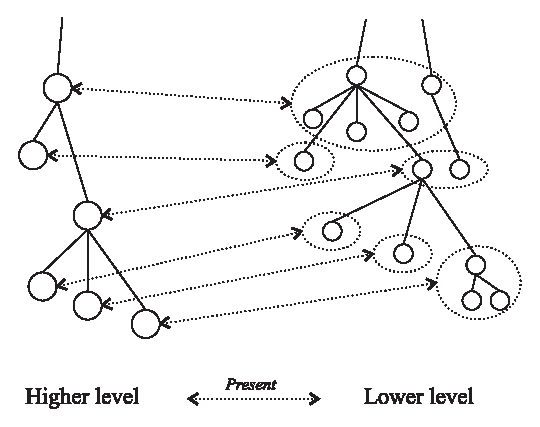
\epsfig{file=pics/eps/mapping.eps, width=2in}
%\begin{verbatim}
%
%     aH        higher level
% bH      cH
% 
%
%                    Layer
%
% 
%     a1L 
% a2L         a3L   Lower level
% bL         cL
%\end{verbatim}
\end{center}
\caption{A mapping between the nodes of two levels.}\label{nodeMapping} 
\end{center}
\end{figure}

\bigskip {\bf The presentation mapping}

\begin{figure}
\begin{center}
\begin{center}
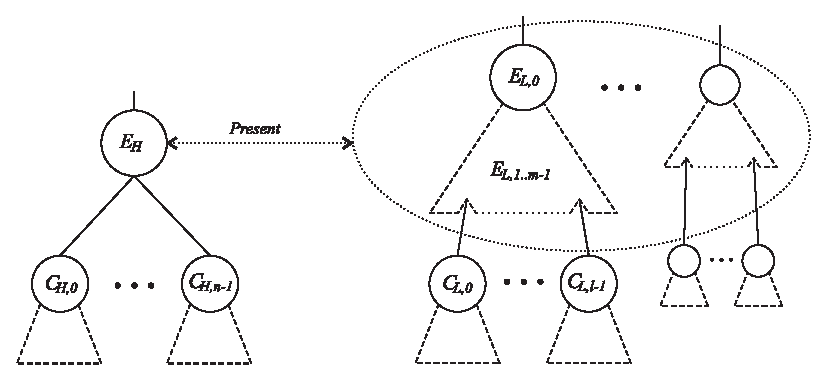
\epsfig{file=pics/eps/presentationEh.eps, width=2in}
%\begin{verbatim}
%                  ..
%                    \
%..                   EL0
%  \                 ELEL.
%   EH       ->     EL..EL.
%  / \             EL....EL. 
% C...C           EL......EL.
%                EL/\EL.EL/\EL.
%                 /__\   /__\
%                    
%\end{verbatim}
\end{center}
\caption{The presentation of element $E_H$.}\label{elementPresentation} 
\end{center}
\end{figure}

First we take a closer look at the downward, or presentation, direction. $Present$ maps each element of the higher level onto zero or more lower level elements, forming zero or more subtrees with holes. \note{is there a name for 'tree with holes'? eg. 'tree segment'?} Figure~\ref{elementPresentation} shows the presentation of one node ($E_H$) in the higher level. $E_H$ is an element in the higher data level that has $n$ children ($C_{H,0}$, \dots, $C_{H,n-1}$). The presentation of $E_H$ is a number of trees (although usually just one) that may consist of several nodes. In the figure, the first tree is shown in more detail. It consists of $m$ nodes is rootet at $E_{L,0}$. 

The $C_{L,0}$, \dots, $C_{L,l-1}$ subtrees in the lower level tree are not part of the presentation of $E_H$. Typically, these are the presentations of the children of $E_H$, but in general they can be (part of) the presentation of any element in the higher level. Alternatively, if a subtree is not part of the presentation of any higher level element, it is part of the extra state of the lower level, which is explained in the next section.

\begin{figure}
\begin{center}
\begin{center}
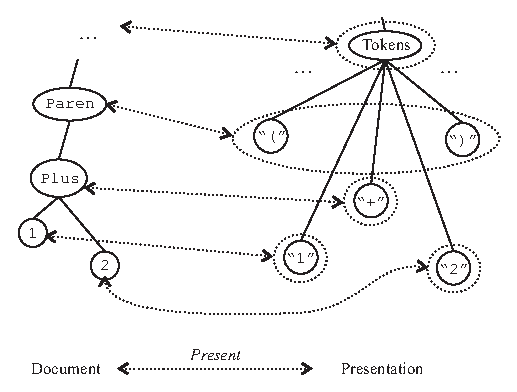
\epsfig{file=pics/eps/presentParenSum.eps}
%
%  ( )       Tk   ( 1+2 )
%   +      Tk ...
%  1 2       .....  
%
\end{center}
\caption{The presentation of a parenthesized sum.}\label{presentExample} 
\end{center}
\end{figure}

Figure~\ref{presentExample} provides a more concrete example of a presentation, taken from a source editor. A parenthesized sum in the enriched document is presented as a set of tokens on the presentation level. The figure shows only a fragment of the enriched document and its presentation. \bc , leaving out the tokens to the left and the right of the expression, as well as the origin of the Tokens element. \ec The tuples in the presentation represent the whitespace of the tokens (line breaks, spaces) as defined in Section~\ref{sect:presLevel}. To the editing user, the expression will be appear as "{\tt (\textvisiblespace 1+2\textvisiblespace )}". The tuples lie outside the dotted ellipses because white space is extra state of the presentation level (see Section~\ref{sect:extraState}). 

\bc
In the example, the resulting presentation is a single tree, but this is not always the case. For example, the evaluation layer in a word processor (see Section~\ref{sect:wordprocessor}), maps each chapter onto an entry in the table of contents, as well as onto the presentation of the chapter itself. Hence, the presentation (in this case the evaluation) of a chapter consists of two separate enriched document trees.
\ec

\bigskip {\bf The translation mapping}

The upward direction, or translation, is slightly more restricted than the downward direction, because a lower level element is allowed to be mapped onto at most one higher level element. Figure~\ref{elementTranslation} schematically shows a translation of a numebr of subtrees rooted at $E_L$. The children in the lower level tree are not mapped onto $E_H$, but may be mapped onto its children (or they may be ignored in the mapping).  Again, the lower level structure is not necessarily a single subtree (with holes); it may consist of several subtrees, e.g. when three presentation tokens \verb|"if"|, \verb|"then"| and \verb|"else"| are mapped onto an \verb|If| node in the enriched document in the parsing phase.


\begin{figure}
\begin{center}
\begin{center}
\epsfig{file=pics/eps/translationEh.eps, width=2in}
%\begin{verbatim}
%
%        EL                 ->    EH
%    EL.......EL               CH ..  CH
% EL  CL  EL  CL  EL
%
%\end{verbatim}
\end{center}
\caption{The translation of the tree rooted at {\tt EL} (beetje dubbel?)}\label{elementTranslation} 
\end{center}
\end{figure}

A consequence of the difference between the presentation and the translation mappings is that even when a lower level element depends on several higher level elements, only one is responsible for its presentation. For example when an element \verb|Word Color String|, representing a colored string, is presented as a string in the specified color. Now the string in the presentation . In order to edit the color

  \note{where does this become important?} \note{example: leaf Color Int $\rightarrow$ colored int. When selecting, either lead or int,  Color affects but is not responsible. can be accessed by special edit ops though.}
\note {maybe say something about 1:n presentation restriction, but also about having $>$1 doc nodes influence same pres.? Or before?}


******** BIG PROBLEM With IntExp  Int. 
Is IntExp translation ES (Then ES is not always a subtree, but can be a segment as well: Paren -- IntExp(es) -- Int )? Then reusing is not as easy anymore.
Or can we translation map onto 2 nodes after all?
Or do we just ignore elts with no pres and rebuild them when translating?

NEED MORE EXPERIENCE!!

%\toHere     % ^^^^^^^^^^^^^^^^^^^^^^^^^^^^^^^^^^^^^
%
%
%*what about parsing to something double?
%*what about IdExp (Id "a")    ->   "a"
%*Isn't this too restrictive?
%* doesn't this make the presentation more simple? translation is hard because several elements need to be 
%regarded.
%if we propagate a value downward as an attribute, it already happens.
%\fromHere  % VVVVVVVVVVVVVVVVVVVVVVVVVVVVVVVVVVVVVVVVVVVV


%* if then else? tokens as list? then focus does not work (no?). tokens as tree?

\bigskip {\bf Duplicates in presentation}
\fromHere  % VVVVVVVVVVVVVVVVVVVVVVVVVVVVVVVVVVVVVVVVVVVV

\note{mention duplicates in translation?}

%* not just because multiple trees: elements may depend on several trees. without duplication.

The presentation of a higher level element may consist of several lower level elements, for example when an \verb|If| node is presented with three tokens. In this case, the three tokens together are translated to the \verb|If| node. However, it is also possible that an element is duplicated in the presentation, in which case two (or more) lower level structures  translate to the same higher level element, possibly creating a conflict. An example of such a copy is the title of a chapter that appears in the table of contents as well as in the presentation of the chapter itself. When the lower level is translated, several alternatives for one element may arise, and a choice has to be made. 
\note{hard to express this as a mapping}

Note that having several lower level elements does not automatically mean that an element is duplicated. The  \verb|If| node is presented on three tokens, but this does not constitute a duplication. Furthermore, translation of duplicates only needs to be dealt with if the duplicate structure is edited on the lower level. If a duplicate only needs to support document editing and no presentation editing, no extra work needs to be done.

The only two layers in which duplicates can be created are the evaluation and the presentation layer. The presentation mappings for the other layers are largely predefined and do not duplicate any structures. To avoind having to deal with duplicates when parsing, duplicating is allowed only at the evaluation layer. This restriction may be lifted in a future version, but for now, if a presentation contains duplicates, the evaluation sheet specifies how the involved structures are duplicated, and the reduction sheet specifies how updates on duplicate structures are handled.

\begin{figure}
\begin{center}
\begin{center}
\epsfig{file=pics/eps/translateToc.eps}
%
%  Chap              Toc
%  "first.."     TokChap      Chap
%                   "first.."     "first.." 
%
\end{center}
\caption{The translation of a word processor document with a table of contents.}\label{translateExample} 
\end{center}
\end{figure}

Figure~\ref{translateExample} shows an example of a duplicated structure in the form of a table of contents for a word processor. On the lefthand side of the figure is a document that contains two chapters, of which only the titles are shown. The enriched document contains both a table of contents tree (\verb|Toc|), as well as a copy of the chapters. The table of contents tree follows the structure of the document, but only contains the title of each chapter rather than the chapter itself. To keep the figure simple, the table of contents only contains chapters and not sections and subsections, but in a real editor the table of contents may reflect the entire document structure. 

The evaluator maps a chapter in the document on a chapter in the enriched document, as well as on a chapter entry in the table of contents tree, leaving out everything but the title in the latter case. The presenter simply presents both the table of contents tree as well as the chapter tree, and does not duplicate any structures. The table of contents example is somewhat complex, because it does not only involve a duplicated presentation, but also a partial presentation (a chapter in the table of contents is shown without its content). Section~\ref{sect:extraState} discusses how partial presentations are handled.

When the enriched document is edited, it is translated (reduced) to an updated document. For duplicate structures, the enriched document contains several alternatives, which may have different translations. In the table of contents example, the alternatives for a chapter title are the title in the table of contents and the title in the chapter. Three situations are possible. Firstly, if none of the alternatives has been edited, all alternative values translate to the same document value, so any one can be chosen. Secondly, if one alternative has been edited, the choice is in favor of the edited element. Hence, if a chapter title is edited in the table of contents, the resulting reduced document contains the updated title. Finally, if more than one value has been edited, an error is signaled to the user. In the example, this happens when the title is edited in the chapter as well as in the table of contents. In this case the edit operation may be forbidden, or one of the values may be chosen.  \note{say that we cannot skip the evaluation layer with this scheme}

Specifying duplications in the evaluation and reduction sheets is not ideal, since the enriched document type now depends on whether or not the presentation contains duplicates. Hence, if a presentation contains several views on a structure, the necessary duplications for these views need to be specified in the evaluation layer. A special facility in for specifying common duplicate presentations, such as tree views on a structure, in the presentation layer is desirable. A possible approach for such functionality is a special parser that can resolve conflicts duplicates during parsing. With such a parser, the whole process of handling duplicates takes place in the presentation layer, and the evaluation layer is not affected. \note{parse (dirty arrangement) $\rightarrow$ dirty presentation? May be tricky as well}

%																
%																
%																
\section{Extra state} \label{sect:extraState}

%SOMEWHERE: when es is hard. If no parent with a presentation is parent then 
% tricky. Hence invisible elements with extra state may lose it during editing.

\note{specify conditions for safety? like in Pierce's lenses stuff?}
\note{mention Pierce paper}

\toHere     % ^^^^^^^^^^^^^^^^^^^^^^^^^^^^^^^^^^^^^

The equations from the previous section assume that a level can be computed from the old values for the two levels together with a sheet and an edit operation on one of the levels. However, this turns out not to be entirely true in the presence of {\em extra state} (also see sections~\ref{sect:editingExtraState}~and~\ref{sect:archExtraState}). If we consider two adjacent data levels, some elements in one level cannot be derived from the other level. 

**
Figure~\ref{layerExtraState} shows two examples levels with the presentation mapping expressed with arrows. The shaded nodes on the higher level have no presentation elements and hence cannot be computed from the lower level during translation. Such elements that cannot be computed from the other level, are referred to as extra state elements.  \note{explain dependency on direction already here?}

% also show a vice versa? with two invariants, it's maybe not logical to show both in one figure

% This is still a copy of  \ref{nodeMapping}
%
\begin{figure}
\begin{center}
\begin{center}
\epsfig{file=pics/eps/prestransESExamples.eps, width=4in}
%\epsfig{file=pics/eps/2levelES.eps, width=4in}
%\begin{verbatim}
%
%        aH        higher level
%  bH         cH
%<shaded>
%
%                    Layer
%
% 
%     a1L 
%          a3L   Lower level
%          cL
%\end{verbatim}
\end{center}
\caption{Two examples of extra state.}\label{layerExtraState} 
\end{center}
\end{figure}
%CAPTION: shaded is extra
%PLAATJE figure of level with arrows, that contains extra state


%This section gives a more precise definition of extra state and specifies how  Furthermore, 
%This section explains : welke info. wanneer gaat het mis. 


%																
\subsection{Extra state in presentation and translation direction}

% One layer: two kinds of extra
Since a presentation of an element may consist of zero or more elements, and a translation consists of at most one, it is possible that an element is not mapped onto any elements in the other level. In that case, the other level simply does not contain the information needed to compute the element, and hence it is part of the former level's extra state. Because the property of extra state depends on the direction of the mapping, we distinguish two kinds of extra state: presentation extra state and translation extra state. The {\em presentation extra state} consists of elements that during presentation cannot be computed from the higher level (the shaded elements at the top level of Figure~\ref{layerExtraState}), and the {\em translation extra state} consists of elements that during translation cannot be computed from the lower level (the shaded elements at the bottom layer of the figure).

% example pres extra
An example of presentation extra state is the whitespace information of a token at the presentation level. This information is not present in the enriched document layer. Instead, the information is reused from the previous presentation of the enriched document. During presentation, tokens are reused, causing the whitespace information to stay the same. In order to do this, we need to know exactly on which presentation elements an enriched document node is mapped in the previous presentation.

% example trans extra
A word processor with an editable table of contents view provides an example of translation extra state.  For sake of simplicity, we will assume that the enriched document only contains the table of contents and not the chapters themselves. This way, we only have to consider the extra state here and not the duplication. Section~\ref{mappingsInLayer} already showed how handle duplications in general, and the same method can be used for the table of contents. 

The evaluator maps chapters, sections, and subsections in the document onto entries in the table of contents tree. An  entry does not contain the content of the corresponding document section, but only its title and entries for its children. During reduction, the table of contents is mapped back onto a complete document, including the parts that are not present in the enriched document. The title of a section comes from the table of contents entry enriched document, but the missing section content is obtained mapping an entry back onto the section that was mapped onto it during the evaluation phase. The section contents, as well as any other child elements that are not in the table of contents, are translation extra state of the evaluation layer.
 
\note{mention that trans ES is more important then pres ES here?}

% even with pres, there can still be extra state
Even if an element \verb|X| is mapped onto one or more elements \verb|Y|$_n$  in the other level, it can still be part of the extra state, if the elements \verb|Y|$_n$ do not constitute enough information to be mapped back onto \verb|X|. Consider for example a presentation of a Haskell source, in which al integers are presented with the string \verb|<Int>|. The integer nodes do have a presentation, but since it does not contain enough information for the backward mapping, the integer nodes are in translation extra state. \note {Is this also the case for focus} \note{Don't know much about this kind of ES yet}
%%%

An important point to note is that extra state with regard to a certain mapping, is extra state for the {\em result} type of the mapping. Hence, presentation extra state for a presentation mapping between $Level_{High}$ and $Level_{Low}$ is part of $Level_{Low}$. Although the term presentation extra state of $Level_i$ may suggest that this concerns state that is used during the presentation of $Level_i$, this is not the case. The extra state of $Level_i$ refers to the extra state with regard to the presentation of the level above ($Level_{i-1}$) on level $Level_i$. The only extra state that involved in the presentation of $Level_i$ is that of its lower neighbor: $Level_{i+1}$


%																
\subsection{One level has two kinds of extra state}

% One level: two kinds of extra
Figure~\ref{layerExtraState} only shows one layer, but since each data level except the document and the rendering is in between two layers, each level between the document and the rendering has two kinds of extra state. Figure~\ref{levelExtraState} shows a data level between two layers. In the figure, both the shaded elements and the bold elements are extra state. The shaded elements are presentation extra state with regard to the higher level, and the bold elements are translation extra state with regard to the lower level. Extra state in one direction is independent of extra state in the other direction, hence an element in the figure can be shaded, bold, shaded as well as bold, or neither. 

\begin{figure}
\begin{center}
\begin{center}
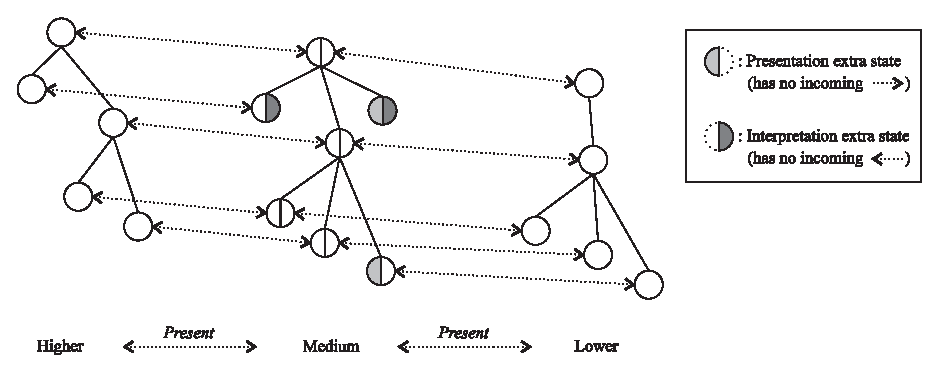
\epsfig{file=pics/eps/3levelES.eps, width=5in}
%\begin{verbatim}
%Level                elt   elt
%                         v    v 
%Level    shaded  elt  bold
%               ^        ^
%Level       elt      elt
%\end{verbatim}
\end{center}
\caption{Presentation and translation extra state in one level.}\label{levelExtraState} 
\end{center}
\end{figure}

% example one level independence of es
The whitespace extra state in tokens provides an example of the fact that the property of extra state in one direction is independent of extra state in the other direction. When the scanner layer translates the layout level, spaces and row transitions between a token's string and the preceding token's string are encoded as whitespace information in the token. Since it can be computed during translation, the whitespace is not part of the translation extra state. On the other hand, when the enriched document is presented on tokens in the presentation level, the whitespace information cannot be computed, and hence it is part of the presentation extra state of the presentation level.
 
\note{also example of one level with both kinds of extra state? Will be somewhat contrived}
%Example Decl, Decl Type Exp., Tree view
%So always Info Pres and Trans. bla core extra:


% equations:
More formally, a data level ($Level_{i}$) can be considered either as the product of the presentation extra state ($Extra_{Pres,i}$) and non-extra state ($Core_{Pres,i}$), or as the product of the translation extra and non-extra state ($Extra_{Trans,i}$ and $Core_{Pres,i}$). The document ($Level_0$) and the rendering ($Level_n$) are special cases, since the document has no presentation extra state, and the rendering has no translation extra state. Expressed with equations, we get:

% Note that pres es for level i is important for pres of level i-1
% and trans es for level i is important for trans of levl i+1
\begin{small}\begin{align*}% \label{sse}
\end{align*} 
\begin{math}
Level_{0} = Core_{Trans,0} \times Extra_{Trans,0}
Level_{n} = Core_{Pres,n} \times Extra_{Pres,n}
\forall 1 \le i \le n-1:  \\
Level_{i} = Core_{Trans,i} \times Extra_{Trans,i} = Core_{Pres,i} \times Extra_{Pres,i} 
%\\
%Present_{i} :: Level_{i} \rightarrow Core_{Pres,i+1} \\
%Translate_{i} :: Level_{i+1} \rightarrow Core_{Trans,i} \\
\end{math}\end{small}


%																
\subsection{Mapping information}



% what extra info to keep
The $Extra$ information in the result types cannot be computed from the arguments. Instead, we try to reuse its previous value. In order to do so, ${\tt translate}$ and ${\tt present}$ get an extra argument which, for each node, contains the nodes it was previously mapped onto. For ${\tt translate}$, the extra argument is of type $Info_{Trans}$, and it is computed by ${\tt present}$. Analogously, ${\tt present}$ gets an extra argument of type $Info_{Pres}$, which is computed by ${\tt translate}$. \note{already mention computation order here?}

\begin{small}\begin{align*}
translate_{i} :: sheet_{Trans} \times Info_{Trans,Low} \rightarrow Level_{Low} \rightarrow Core_{Trans,High}  \times Extra_{Trans,High}  \times Info_{Press,High}\\
present_{i} :: sheet_{Pres}  \rightarrow Info_{Pres,High} \rightarrow  Level_{High} \rightarrow Core_{Pres,Low} \times Extra_{Pres,Low}   \times Info_{Pres,Low} \\
%\\
%level'_{High} = {\tt translate}~sheet_{Trans}~info'~level'_{Low}\\
%level''_{Low} = {\tt present}~sheet_{Pres}~level''_{High}\\
%\\
%Present_{i} :: Level_{i} \rightarrow Core_{Pres,i+1}\\
%Translate_{i} :: Level_{i+1} \rightarrow Core_{Trans,i}\\
\end{align*} 
\end{small}
{\centering ()\\}


% example in picture 
Figure~\ref{mappingInfo} shows two examples of the $Info$ argument. The lefthand side shows the situation at the presentation layer of a Haskell source editor during presentation.  The enriched document element \verb|If|  was presented on the three tokens in the presentation level. The downward arrows represent $Info_{Pres,High}$, whereas the upward arrows are the translation information $Info_{Trans, Low}$. The dotted arrows represent $Info_{Trans,High}$ (upward) and $Info_{Pres,Low}$ (downward), which are not used in this layer. The whitespace nodes in the presentation level are presentation extra state, that has to be reused on presentation. \note{more detail on reuse?}

The righthand side of the figure shows the evaluation layer of a word processor during translation. The document is a \verb|Chapter| element containing two \verb|Section| children, which is mapped onto a table of contents structure in the evaluation level. Again, downward arrows are $Info_{Pres,High}$ and upward arrows are $Info_{Trans,Low}$. \note{mention there is no $Info_{Trans,High}$?} In this case, the document contains translation extra state, since the contents of the chapter and sections cannot be computed from the enriched document.  \note{more detail on reuse?}

\begin{figure}
\begin{center}
\begin{center}
\begin{footnotesize}
\begin{verbatim}
Enriched Document:                       Document:                                                                                            
                                                                                            
                  If                         Chapter "chapter 1" {"this is bla bla bla..."} 
            / /   | |   \\                      v       v                                     
           v v    v v    vv              Sect "1" {"..."}     Sect "2" {"..."}                
       ^           ^           ^           |   /                    \   |                            
      /    ^       |   ^        \  ^       v  v          ^  ^        v  v                          
    Token /      Token |      Token \                    |  |                             
 {WS} "if"    {WS} "then"  {WS} "else"      ChapterTocEntry "chapter 1"                     
                                          ^              ^                 ^   ^              
Presentation:                            SectionTocEntry "1"  SectionTocEntry "2"           
                                                                                            
                                         Enriched Document:                                 

----------                                                                        
legend   ^ is pres info       v is trans info     {node} is extra state            
                                                                                  
\end{verbatim}  
\end{footnotesize}                                                                  
\end{center}                                                                      
\caption{Mapping information.}\label{info}                          
\end{center}                                                                      
\end{figure}

%??? 
%Mapping is to the node for reusing. Mapping to path is for associating doc edits with presentation parts.
%If things are moved, the paths are no longer meaningful (nodes are). Before doc op, always fix paths by parsing.


%What about keeping list [ID->Info?] that switches and is not part of level.
We choose to make the mapping information part of the $Level$ type. The reason for this is that both adjacent layers may update a level, and therefore also affect the mapping information on the level. \note{need an example?} With the mapping information in the level types, ${\tt present}$ and ${\tt translate}$ do not need additional arguments anymore.

Except for the top and bottom levels, all levels contain presentation and translation information. The top level is never the result of a presentation mapping, and hence has no presentation information, whereas the bottom level has no translation information. The definition of $Level_i$ and the types of $present_i$ and $translate_i$ become:

\begin{small}\begin{align*}% \label{sse}
\end{align*} 
\begin{math}
Level_{0} = (Core_{Trans,0} \times Extra_{Trans,0}) \times Info_{Trans,0}
Level_{n} = (Core_{Pres,n} \times Extra_{Pres,n}) \times  Info_{Press,n}
\forall 1 \le i \le n-1:  \\
Level_{i} = (Core_{Trans,i} \times Extra_{Trans,i}) \times Info_{Pres,i} \times  Info_{Trans,i}\\  
               = (Core_{Pres,i} \times Extra_{Pres,i})  \times Info_{Pres,i} \times  Info_{Trans,i}\\  
\\
translate_{i} :: sheet_{Trans} \rightarrow Level_{Low} \rightarrow Level_{High}\\
present_{i} :: sheet_{Pres}  \rightarrow  Level_{High} \rightarrow Level_{Low}\\
\end{math}\end{small}

% computation order
The mapping information that is used by ${\tt present}$ is computed by ${\tt translate}$ and vice versa. As a consequence, only one kind of mapping information is guaranteed to be valid. After presentation, the translation mapping is correct, but the presentation mapping may be incorrect, whereas after translation, the presentation information is correct, but the translation information may be incorrect. However, this does not cause any problems since a level is presented before its lower neighbor is translated, and vice versa. \note{when we have higher level edit ops, this will become a problem}

It may seem more appropriate that presentation mapping information is a result of the presentation, rather than the translation, since it concerns information about the presentation of the level and not its translation, but this is not the case. Besides causing ${\tt present}$ to return two levels, rather than one, there is another reason why the information cannot be computed by ${\tt present}$. After a level is presented, the lower level may be updated by the lower adjacent layer. If ${\tt present}$ computes the mapping information in the higher level, which refers to the lower level, then this information may not be correct anymore after a lower level update. By computing the mapping information during translation, the problem is avoided, since after its translation, the lower level is not edited before the higher level is presented again. The same thing holds for ${\tt translate}$.

\note{does give a problem when mappings are not inverse}
\note{eg. "chess:" "board" -> ChessBoard. Now ChessBoard has wrong pres info when presented on an image instead of tokens}
% if pres.translate not is id, then translate map is different from pres map. ES is not valid. translate.pres is always id




%																
%																
%																
\section{Maintaining the presentation invariant during editing}

% say that now we develop an actual function present/translate that implements the mapping

During editing, data levels are updated as a result of user interaction. When a level changes, the adjacent level needs to be updated to establish the appropriate invariant. We specify two mapping functions  
${\tt present}$ and ${\tt translate}$ that compute new levels. On a higher level update, ${\tt present}$ computes a lower level that establishes the presentation invariant. Similarly, on a lower level update, a new higher level is computed by the ${\tt translate}$ mapping, establishing the translation invariant. 

We can express this with two equations:

\begin{math}
{\tt present} :: Level_{High} \rightarrow Level_{Low} \\
{\tt translate} ::  Level_{Low} \rightarrow Level_{High} \\
level_{Low} = Present~level_{High}\hfill \text{\{Precondition\}}\\
level'_{High} = {\tt translate}~level'_{Low}\\
level'_{High} = Translate~level'_{Low}\hfill \text{\{Intermediate condition\}}\\
level''_{Low} = {\tt present}~level''_{High}\\
level''_{Low} = Present~level''_{High}\hfill \text{\{Postcondition\}}\\
\end{math}
%INV seems a bit silly, but this will change
% precondition not used yet

\bigskip {\bf Presentation/Translation sheets}
** However = verkeerde woord.
However, this set of equations gives an oversimplified view of the situation, as it implies that presentation of the higher data level depends only on the higher level itself and the presentation mapping. A similar thing holds for the translation. We might wish to influence how a level is presented without altering the data level or taking an entirely different presentation mapping. A more elegant solution is to have a separate style sheet that specifies the presentation and pass that style sheet as an argument to the function ${\tt present}$ and ${\tt translate}$. \note{explain separation of data and presentation} \note{mention recompiling?} Therefore, we parameterize the presentation and translation functions with a {\em sheet} argument. The presentation sheet has the abstract type $Sheet_{Pres}$, and the translation sheet is of type $Sheet_{Trans}$.

\begin{math}
{\tt present} :: Sheet_{Pres} \rightarrow  Level_{High} \rightarrow Level_{Low} \\
{\tt translate} :: Sheet_{Trans} \rightarrow  Level_{Low} \rightarrow Level_{High} \\
level_{Low} = Present~level_{High}\hfill \text{\{Precondition\}}\\
level'_{High} = {\tt translate}~sheet_{Trans}~level'_{Low}\\
level'_{High} = Translate~level'_{Low}\hfill \text{\{Intermediate condition\}}\\
level''_{Low} = {\tt present}~sheet_{Pres}~level''_{High}\\
level''_{Low} = Present~level''_{High}\hfill \text{\{Postcondition\}}\\
{\tt translate}~sheet_{Trans}  \cdot {\tt present}~sheet_{Pres} = id_{High}\\
\end{math}
\note{also put id condition in previous invariant? And add the PRES TRANS one too?}

The sheet parameter contains information about how to present or translate the elements of the respective data levels. The presentation sheet for the presentation layer specifies the presentation of the enriched document. At the evaluation layer, the presentation sheet is called the evaluation sheet, which specifies the computation of the derived values. The translation sheet at the presentation level specifies the parser, and at the evaluation layer it specifies the reducer, which maps updates on derived structures back onto updates on the document. Note that the sheets do not appear in the abstract $Present$ and $Translate$ functions, as these represent the intended presentation and translation mappings that we implement with the functions ${\tt present}$, ${\tt translate}$ and the respecitive sheet parameters. \note{scanner sheet}

Although a layer has two sheets, the two are closely related as they have to satisfy the
$Translate \cdot Present = id_{High}$ condition. For simple editors, the sheets at the evaluation and presentation layer may even originate from a single specification. However, we choose to represent the sheets as two separate entities because the mappings they define do not have to be the same. \note{Say this differently, of course the mappings are not the same. trans is more liberal? trans is not injective?} Furthermore, the two sheets may be specified in completely different formalisms. For example, at presentation level, the presentation of the document may be specified using an attribute grammar, whereas the parser may be specified using parser combinators.






%																
%																
%																
\section{Maintaining extra state during editing} \label{sect:maintainingExtraState}

** meer intro

%***** WHAT ABOUT PRES . TRANS = ID?

% mapping we have is not good enough
The available mapping functions $Present$ and $Translate$ both go from $Level$ to $Core$. However, the editor layer has to realize mappings between levels, and hence we need functions ${\tt present}$ and ${\tt translate}$ that have a result type of $Core \times Extra$:
% not for top and bottom

\begin{math}
{\tt translate} :: Sheet_{Trans} \rightarrow Level_{Low} \rightarrow Core_{Trans,High}  \times Extra_{Trans,High} \\
{\tt present} :: Sheet_{Pres} \rightarrow Level_{High} \rightarrow Core_{Pres,Low} \times Extra_{Pres,Low} \\
\end{math}

% what extra info to keep
The $Extra$ information in the result types cannot be computed from the arguments. Instead, we try to reuse its previous value. In order to do so, ${\tt translate}$ and ${\tt present}$ get an extra argument which, for each node, contains the nodes it was previously mapped onto. For ${\tt translate}$, the extra argument is of type $Info_{Trans}$, and it is computed by ${\tt present}$. Analogously, ${\tt present}$ gets an extra argument of type $Info_{Pres}$, which is computed by ${\tt translate}$. \note{already mention computation order here?}


%																
\subsection{Safety of extra state}
\note {where to say:  new nodes have no es, use initial value}

Because the reuse of extra state depends on the mapping information, extra state may be lost if the mapping information is not valid. There are in two situations in which the mapping information can be invalid.  

First of all, a level may be updated in such a way that the mapping information that was computed at the previous presentation or translation, is no longer correct. An example is when a document edit operation in a Haskell source editor changes a sum to a product. The old presentation mapping in invalid, since it points to the presentation of the sum. In this case, because of the similarity between the presentations of a sum and a product, the tokens can be reused, but if the updated node has a completely different presentation, then the layout information of the tokens is lost.

The second situation in which the mapping information may be invalid, is if ${\tt present} \cdot {\tt translate}$ is not identity function for a node. \note{say this some other way?} An example is found in a source editor that provides graphical presentations for some of its tokens (eg. $\rightarrow$ for the token \verb|"->"|). If a \verb|"->"| token is parsed, the mapping information in the resulting enriched document node points toward the textual arrow. However, if the enriched document is presented, the presentation contains a graphical arrow, and hence the mapping information with respect to the arrow token is incorrect. In such a case, the presentation function itself must take care of reusing extra state from the textual arrow token for the graphical arrow token.

The reverse situation does not occur, since we require that ${\tt translate} \cdot {\tt present}$ is identity for a node. \note{add this to the invariants}

In case the extra state cannot be restored, it is set to an initial value. Thus, if an entry is added to a table of contents in the enriched document of a word processor, a chapter (or section) without any content is added to the document. Similarly, if a document edit operation in a source editor adds a new structure to the document, its presentation gets a default layout.

The responsibility of restoring extra state and handling problem situations, currently lies within each layer itself. Restrictions on the presentation and translation mappings could possibly guarantee the safety of extra state, but currently, no such restrictions have been established. However, the fact that safety of extra state cannot be guaranteed in general, does not actually have to cause a problem. Since presentation extra state generally consists of non-essential information, it is not a big problem that in some rare cases, it is reset to a default value. \note{mention this difference somewhere before} Translation extra state, on the other hand, does represent essential information, but by restricting the edit behavior on presentations that have translation extra state, it can be protected. For example, the edit behavior on a table of contents can be restricted to updates on titles, and insertion and deletion of entire entries. This way, the corresponding section nodes in the document are never lost. Of course, it is still possible to delete a chapter by removing its table of contents entry, but this is a choice made by the editor designer. 


\note{can we always tell that extra state was lost?}

%Now left to editor. During pres, do we have old node? And what about trans? Do we have old pres?
%Would be nice if we could guarantee safety. When? context free presentation?
%list delete is in general no problem  Or parent if context sensitive presentation.

%higher level update without lower level translation gives problem. but not mentioned here, only in layered archs
%lower level update without higher level pres?   is this not just editing and skipping higher layers?


%																
\subsection{conclusions}
% the final equations

The equations that describe the behavior of ${\tt present}$ and ${\tt translate}$ in the presence of extra state are:

\begin{small}\begin{align*}% \label{sse}
Level_{0} = Core_{Trans,i} \times Extra_{Trans,i} \times Mapping_{Pres,i}\\
Level_{n} = Core_{Pres,i} \times Extra_{Pres,i} \times Mapping_{Trans,i}\\
\forall 1 \le i \le n-1:  \\
Level_{i} = Level_{i} \times Mapping_{Trans,i} \times Mapping_{Pres,i}\\
Level_{i} = Core_{Trans,i} \times Extra_{Trans,i} = Core_{Pres,i} \times Extra_{Pres,i} \\
\\
translate_{i} :: sheet_{Trans,i} \rightarrow Level_{i+1} \rightarrow Level_{i}\\
present_{i} :: sheet_{Pres,i}  \rightarrow  Level_{i} \rightarrow Level_{i+1}\\
\\
%level_{Low} = Present~level_{High}\hfill \text{\{Precondition\}}\\
level'_{High} = {\tt translate}~sheet_{Trans}~level'_{Low}\\
%level'_{High} = Translate~level'_{Low}\hfill \text{\{Intermediate condition\}}\\
level''_{Low} = {\tt present}~sheet_{Pres}~level''_{High}\\
%level''_{Low} = Present~level''_{High}\hfill \text{\{Postcondition\}}\\
{\tt translate}~sheet_{Trans}  \cdot {\tt present}~sheet_{Pres} = id_{High}\\
\\
Present_{i} :: Level_{i} \rightarrow Core_{Pres,i+1}\\
Translate_{i} :: Level_{i+1} \rightarrow Core_{Trans,i}\\
\end{align*} 
\end{small}
{\centering ()\\}

The model for extra state presented in this section only shows what information must be kept track of by a layer in order to support extra state. It does not specify how to keep track of the extra information, nor how to handle conflict situations, or loss of extra state. This is left to the individual layers. Furthermore, the reuse of extra state only works for extra state that is attached to a non-extra state parent node. 

Still, besides these restrictions, the model works for specifying the whitespace extra state for token presentations as well as translation extra state for editing partial presentations. Further research is required to established restrictions on the presentation and translation mappings, that can guarantee safety of extra state. Furthermore, a method for handling extra state that is not attached to specific parent nodes is desirable. Finally, experience with building editors with Proxima, as well as using these editors will provide more instances of extra state, and information on how to solve conflict situations.

% Not enforced by the invariants! Need more detailed stuff on element level. Future research.

%Remember ES on parsing stuff is fragile
%unless strong restrictions. important for translation direction
%layout is an example. things like order are harder. extra layer?
%Many possibilities not researched yet.



%Have to figure out more about Focus ES, and other non node ES.
%order changes are not yet clear!


%																
\section{Incrementality}
% meer uitleg?: no choice on inc, even memo may be used, but do need old level for that.

The proposed ${\tt present}$ and ${\tt translate}$ mappings from the previous sections take one level as argument and return another. This means that each time a mapping is computed, the entire result level needs to computed. However, changes in one level frequently only cause local changes in the other level. For example, if the presentation of a paragraph in a word processor is changed, the corresponding enriched document update only concerns that single paragraph. Hence, we will change the mapping functions in such a way that instead of mapping one level onto another, they map an edit operation on one level onto an edit operation on the other level. \note{explain that this is at least as powerful as non-incremental? ({\tt $\backslash$(Set lvl) -$>$ Set lvl')}}

Figure~\ref{fromLevelToOp} shows the difference between a translation mapping between levels and a mapping between edit operations. On the lefthand side is the mapping between levels, in which a new higher level is mapped onto an updated lower level. On the righthand side, the mapping between edit operations is shown. The values for the updated levels are computed by applying a function
 ${\tt update} :: Edit_\alpha \rightarrow \alpha \rightarrow \alpha$ to the edit operation and the level. A 
 ${\tt present}$ function between edit operations instead of levels can be specified similarly.

\begin{figure}
\begin{small}
\begin{center}
\begin{center}
\begin{small}
\bigskip \noindent
\xymatrix{
                               &                &                                      & \data{$e_{Level_{High}}$} \ar[dr]        &                           &                        \\
\data{$level'_{High}$}         &                & \data{$level_{High}$} \ar[rr]\ar[dr] &                                          & \component{${\tt update}$} \ar[r] & \data{$level'_{High}$} \\
\component{${\tt translate}$} \ar[u] & {\rm becomes: }&                                      & \component{${\tt translate}$}  \ar[uu]         &                           &                        \\
\data{$level'_{Low}$}   \ar[u] &                & \data{$level_{Low}$}  \ar[rr]\ar[ur] &                                          & \component{${\tt update}$} \ar[r] & \data{$level'_{Low}$}  \\
                               &                &                                      & \data{$e_{Level_{Low}}$} \ar[uu] \ar[ur] &                           &                        \\
}
\end{small}
\end{center}\caption{Level to level versus edit operation to edit operation }\label{fromLevelToOp} 
\end{center}
\end{small}
\end{figure}


% there is PRES, which is a level thing, pres, which is incremental, and also presLevel
% pres will work on mappings, presLevel won't. Is this PRES? or do we keep PRES abstract
The arrows going from the higher and the lower level to ${\tt translate}$ in the righthand side of Figure~\ref{fromLevelToOp}, are necessary because in some cases, it is hard to map a lower level edit operation onto a higher level edit operation without reference to the respective data levels. If such a mapping is not available, but there is a non-incremental mapping between levels, then the computation sketched in Figure~\ref{computeOps} can be used to obtain a mapping between edit operations. The figure shows how a function ${\tt translate} :: Edit_{Level_{High}} \rightarrow Edit_{Level_{Low}}$ can be constructed when only a function with type ${\tt translate'} :: Level_{High} \rightarrow Level_{Low}$  is available. In the figure, the edit operation is applied as an update to the old higher level, using the function ${\tt update}$. A new lower level is then computed by applying ${\tt translate'}$ to the updated updated higher level. Finally, the incremental lower level update is computed by taking the difference of the updated lower level and the original. Of course, this is only a sketch, and the difference function does not exist in general, but for some editors, it will be a feasible solution. In order to allow this kind of computation, ${\tt translate}$ needs the values of the higher and lower level as arguments.

\begin{figure}
\begin{small}
\begin{center}
\begin{center}
\begin{small}
\bigskip \noindent
\xymatrix{
 \data{$e_{Level_{High}}$}  & \component{diff} \ar[l] & \data{$Level_{High}$} \ar[l] \\
 & \data{$Level_{High'}$} \ar[u] & \\ 
 & \component{$translate'$} \ar[u] & \\
 & \data{$Level_{Low'}$} \ar[u] & \\
\data{$e_{Level_{Low}}$} \ar[r] & \component{${\tt update}$} \ar[u] & \data{$Level_{Low}$} \ar[l]
% same thing for present
% \data{$e_{Level_{High}}$} \ar[r] & \component{${\tt update}$} \ar[d] & \data{$Level_{High}$} \ar[l] \\
% & \data{$Level_{High'}$} \ar[d] & \\ 
% & \component{$Presenter$} \ar[d] & \\
% & \data{$Level_{Low'}$} \ar[d] & \\
%\data{$e_{Level_{Low}}$} & \component{diff} \ar[l] & \data{$Level_{Low}$} \ar[l]  \\
}
\end{small}
\end{center}\caption{Computation of $e_{High}$ from $e_{Low}$ (add box: and say trans = [upd trans' diff] )) }\label{computeOps} 
\end{center}
\end{small}
\end{figure}

For the presentation mapping, a similar computation can be performed. Hence, ${\tt present}$ also needs the values of the two levels. 

Before we give the invariants for the incremental versions of the layer functions, we introduce a short-hand notation for the ${\tt update}$ functions. Especially for larger computations, these functions clutter the diagrams, due to crossing arrows and the many rather uninformative appearances of ${\tt update}$. In the normal notation, an update $data' = {\tt update}~e_{Data}~data$, for values 
$data, data' :: Data$, is represented as:\\

\begin{small}
\xymatrix{
                               &  \data{$e_{Data}$} \ar[d] \\
\data{$data$} \ar[r] &  \component{${\tt update}$} \ar[r] & \data{$data'$} \\
}
\end{small}

\smallskip
Because an edit operation on a value of type $Data$ can also be regarded as a function of type 
$Data \rightarrow Data$, we use a squiggly arrow notation that leaves the function ${\tt update}$ implicit:\\

\begin{small}
\xymatrix{
\data{$data$} \ar@{~>}[r] & \data{$e_{Data}$} \ar@{~>}[r] & \data{$data$} \\
}
\end{small}

Figure~\ref{incrementalTranslate}, shows the righthand side of Figure~\ref{fromLevelToOp} using the new notation.

\begin{figure}
\begin{small}
\begin{center}
\begin{center}
\begin{small}
\bigskip \noindent
\xymatrix{
\data{$level_{High}$} \ar@{~>}[r]\ar[dr] & \data{$e_{Level_{High}}$} \ar@{~>}[r] &\data{$level'_{High}$} \\
                                         & \component{${\tt translate}$}  \ar[u]           &                           &                           \\
\data{$level_{Low}$}  \ar@{~>}[r]\ar[ur] & \data{$e_{Level_{Low}}$}  \ar[u] \ar@{~>}[r]          & \data{$level'_{Low}$}  \\
}
\end{small}
\end{center}\caption{Incremental ${\tt translate}$.}\label{incrementalTranslate} 
\end{center}
\end{small}
\end{figure}

In addition to the extra parameters, and the change from level to edit operation, the equations for the incremental versions of ${\tt present}$ and ${\tt translate}$ also contain a number of explicit ${\tt update}$ functions. Furthermore, note that compared to ${\tt translate}$, the order of the level parameters for         ${\tt present}$ is swapped (ie. first the higher and then the lower level) since the direction of the mapping is also swapped.
 
% PRES and TRANS are not incremental
\begin{math}
{\tt present} :: Sheet_{Pres} \rightarrow  Level_{High} \rightarrow Level_{Low}  \rightarrow Edit_{Level_{High}} \rightarrow Edit_{Level_{Low}} \\
{\tt translate} :: Sheet_{Trans} \rightarrow  Level_{Low} \rightarrow Level_{High} \rightarrow  Edit_{Level_{Low}} \rightarrow Edit_{Level_{High}} \\
\text{\{\}}\\
\\
level_{Low} = Present~level_{High}\hfill \text{\{Precondition\}}\\
level'_{Low} = {\tt update}~e_{Level_{Low}}~level_{Low}\\
e_{Level_{High}} = {\tt translate}~sheet_{Trans}~level_{Low}~level_{High}~e_{Level_{Low}} \hfill 
\text{\{\}}\\
level'_{High} = {\tt update}~e_{Level_{High}}~level_{High}\\
level'_{High} = Translate~level'_{Low}\hfill \text{\{Intermediate condition\}}\\
\\
level''_{High} = {\tt update}~e'_{Level_{High}}~level'_{High}\\
e'_{Level_{Low}} = {\tt present}~sheet_{Pres}~level'_{High}~level'_{Low}~e'_{Level_{High}} \hfill 
\text{\{\}}\\
level''_{Low} = {\tt update}~e'_{Level_{Low}}~level_{Low}\\
level''_{Low} = Present~level''_{High}\hfill \text{\{Postcondition\}}\\
\end{math}

Two updates take place on the higher level, and two on the lower level. However, if we look at Figure~\ref{computeOps}, we can see that a higher level update is performed in the computation of
 ${\tt present}$. Thus, besides $e'_{Level_{Low}}$ an implementation of ${\tt present}$ may also return $level''_{High}$. \note{say the the remaining updates disappear because of composition} Similarly, ${\tt translate}$ may return $e'_{Low}$. \note{Mention that on composition two of the four updates can be dropped?}

%However, because a layer does not exist on its own, but is composed with other layers (as will be explained 
%in the next Chapter), an adjacent layer will also do an update on the level. Hence


%																
\section{Conclusions}

In one level,  mapping info to higher and lower (except for doc \& rendering), furthermore, the tree can can be regarded bla.

-mapping for pres = Mapping pres. doc only has mapping pres, ren only mapping trans. Core\&extra are wrt mapping of which level is destination. level is extra for pres from higher and trans from lower. Doc only has trans  and ren only pres.



A Proxima Layer:
plaatje met alle in en uitvoer van 1 level


Parse errors in tokens requires trans update on lower. Different model. First research necessary if this way of parsing is good

Proxima offers possibility of solving, not always solution. non tree stuff, or inserted nodes? (redundant parens, tree order) Many problems, need to be solved, but then they can be implemented.




%																
%																
%																
%\section{Bidirectional mappings}
%
%What do we lose exactly by not keeping the mappings
%
%reuse original trees, update mappings upward and downward



%																
%																
%																
%\section{Consequences for each layer}
%Layer examples.
%In arrangement, mappings automatic, formatters etc. rest is easy
%
%In rendering, no mappings
%Doc-Pres, left to editor builder. what happens if we don't do them
%tokens contain origin in edoc. identity is reused. What if type changes?
%
%
%Using caching of parsers and presenters to preserve the mapping
%-- List support for these mappings	% 5
\setcounter{chapter}{5} \chapter{Layered Editor Architectures}
\label{chap:layeredArchs}

bla

* Order: layered, single  or single, layered?
* layers, single. PROBLEM edit and diff model must be explained, and is typical single layer stuff
                         GOOD: edit process is already explained before single
                         
* single, layers. PROBLEM assumes edit ops in and out
                                        edit process not explained
                         GOOD: Final bits of layered can give the complete thing, including one layer
                                    edit/diff stuff explained.

single, layers: probably the best choice. edit model is already a bit explained previously. and one of the reasons for edit ops instead of levels is that single layer needs this.
                                    


* fix gesture to edit Rendering, unless gesture becomes something special
* rendering or presentation? Rendering is more clear, but editing the rendering does not make sense. (maybe just explain)

* MAAK DUIDELIJK WAT IN EN UIT GAAT, BIJ INC ZIJN ALLE LEVELS IN (BIJ ANDERE ALLEEN DOC?)
HOE HEEFT PRE HIERMEE TE MAKEN? pre geeft geen berekening, maar alleen verband, dus zelfs als level i opgeleverd door pre, dan nog is het invoer

{\em *** Version: \today~ ***}

- Numbering 0 = doc, downwards like lines on a page.



** ?Add an $lower = EDIT~levels~gesture$ condition that states the result is what we mean with the gesture?

In this chapter, compose the layers from the previous chapter. First make a presentation system (not an editor), add layers. Then editor with layers. Finally, editor with the layers from previous chapter. And some more stuff for typical layer functionality. (skipping, and higher level edit ops)


%																
%																
%																
\section{Presentation system}

Presentation systems are applications that provide a user with some kind of view  on a data structure. Examples of presentation systems are pdf-viewers, image viewers, and web browsers, although the latter also have functionality for accessing non-local documents. Because an editor can be seen as  a presentation system with extra functionality  for editing the presented data, we will first develop a number of invariants that model the architecture of a presentation system, and in the next section rework the invariants to model an editor.


???
In this section, as well as in the following two, we will follow the same line of reasoning while constructing the invariants. First, we consider a simple case, in which the rendering of a document is computed in one single step. Secondly, the functions mapping the document to the rendering and the functions that map the edit gestures on the rendering to document updates are split in a number of subfunctions, each handling a specific step in the mapping process. And finally, we will extend the invariant to support the local state that was mentioned in the previous section. In some cases, a first attempt is given for the invariant, which is refined afterwards. 
??


%																
\subsection{Single stage presentation}

Suppose that there is a function $present :: Document \rightarrow Rendering$ that maps a $document$ of type $Document$ to a $rendering$ of type $Rendering$. We formally define the relation between the document and the rendering with the invariant:

\begin{small}
\bigskip \noindent
\xymatrix{
\data{$document$}\ar[d]	\\
\component{$present$} \ar[d] \\
\data{$rendering$}	 \\
}
\end{small}

\begin{small}\begin{align*}
present & :: Document \rightarrow Rendering \\
\end{align*}
\begin{math}
rendering = present~document
\hfill \text{\{Compute Rendering\}}
\end{math}\end{small}

{\centering (Invariant 2: One stage presentation, Final)\\}\vspace{1em}


%																
\subsection{Layered presentation}


\begin{small}
\bigskip \noindent
\xymatrix{
 \data{$level_{0}$}\ar[d]  \\
\component{$present_{0}$} \ar[d]\\
\data{$level_{1}$} \ar@{.>}[dd]   \\
		\\
\data{$level'_{n-1}$}\ar[d]	\\
\component{$present_{n-1}$} \ar[d]\\
\data{$level_{n}$}\\
}
\end{small}



\begin{small}
\begin{align*} % \label{lpupdate}
present_i & :: Level_i \rightarrow Level_{i+1} \\
\end{align*}
\begin{math}
\forall 0 \le i \le n-1: \\
level_0 = document \\
level_{i+1} = present_i~level_i\\
rendering = level_n \hfill \text{\{Compute Rendering\}}
\end{math}\end{small}

{\centering (Invariant 4: Layered presentation, Final)\\}\vspace{1em} 


%																
\subsection{Layered presentation with local state}


\begin{small}\begin{align*} % \label{llp}
present_i & :: Sheet_i \rightarrow Level_i \rightarrow Level_{i+1}\\
\end{align*}
\begin{math}
\forall 0 \le i \le n-1: \\
level_{i+1} = present_i~sheet_i~level_i
\hfill \text{\{Compute Rendering\}}
\end{math}\end{small}

{\centering (Invariant 5: Layered presentation with local state)\\}\vspace{1em}



\begin{figure}
\begin{small}
\begin{center}
\begin{center}
\end{center}\caption{ The edit process}\label{editprocess} 
\end{center}
\end{small}
\end{figure}


%																
%																
%																
\section{Editor}

plaatje van edit proces, show get gesture, update ...


%																
\subsection{Single stage editor}


\begin{small}
\bigskip \noindent
\xymatrix{
\data{$document$}\ar[d]	& 			& \data{$document'$}\ar[r] 		& \data{$document''$}\ar[d]  \\
\component{$present$} \ar[d] &			& \component{$translate$} \ar[u]	& \component{$present$} \ar[d]\\
\data{$rendering$} \ar[r]	& \component{update} \ar[r] 	& \data{$rendering'$}\ar[u] 		& \data{$rendering''$}  \\
			& \data{$gesture$} \ar[u]	&				& 	 	
}
\end{small}




\begin{small}\begin{align*}% \label{sse}
update & :: Edit_\alpha \rightarrow \alpha \rightarrow \alpha \\
present & :: Document \rightarrow Rendering \\
translate & :: Rendering \rightarrow Document \\
\end{align*} 
\begin{math}
rendering = present~document	\hfill \text{\{Precondition\}} \\
rendering' = update~gesture~rendering	\hfill \text{\{Update rendering\}} \\
document' = translate~rendering' 	\hfill \text{\{Compute updated document\}}\\
document'' = document'		\\% \hfill \text{\{Update Document\}} \\
rendering'' = present~document''	\hfill \text{\{Postcondition + Compute rendering'\}} \\
\end{math}\end{small}
{\centering (Invariant 6: One stage editor, 1st attempt)\\}

- niet reeel, rendering = presentation, assume eg text only, translation is parser.

- explain ' \& ''

- twee keer update op rendering, eerste keer bv insert keywords als text, daarna met mooie opmaak. niet op doc
* somewhere translate.pres does not need to be id. can be, 01 -> 01 have to store extra info, however editor can choose to do something else, normalize, nice formatting.

- merk op dat doc'' = doc, maakt berekening eleganter

* Add correctness? met EDIT \& PRESENT? Maakt ook trans/pres volgorde in inc duidelijker


%																
\subsection{Layered editor}


\begin{small}
\bigskip \noindent
\xymatrix{
 \data{$level_{0}$}\ar[d] 	& 			& \data{$level'_{0}$}\ar[r] 		& \data{$level''_{0}$}\ar[d]  \\
\component{$present_{0}$} \ar[d]&			& \component{$translate_{0}$} \ar[u]	& \component{$present_{0}$} \ar[d]\\
\data{$level_{1}$} \ar@{.>}[dd]	& 		 	& \data{$level'_{1}$}\ar[u] 		& \data{$level''_{1}$} \ar@{.>}[dd]  \\
				&			& 				& 	 		\\
\data{$level'_{n-1}$}\ar[d]	&	 		& \data{$level'_{n-1}$}\ar@{.>}[uu] 	& \data{$level''_{n-1}$}\ar[d]  \\
\component{$present_{n-1}$} \ar[d]&			& \component{$translate_{n-1}$} \ar[u]	& \component{$present_{n-1}$} \ar[d]\\
\data{$level_{n}$} \ar[r]	& \component{update} \ar[r] 	& \data{$level'_{n}$}\ar[u] 		& \data{$level''_{n}$}  \\
			& \data{$gesture$} \ar[u]	&				& 	 	
}
\end{small}


\begin{small}\begin{align*} % \label{le}
update & :: Edit_\alpha \rightarrow \alpha \rightarrow \alpha \\
present_i & :: Level_i \rightarrow Level_{i+1} \\
translate_i & :: Level_{i+1} \rightarrow Level_i \\
\end{align*} 
\begin{math}
\forall 0 \le i \le n-1:  \\
level_{i+1}= present_i~level_i		\hfill \text{\{Precondition\}} \\
level'_{i} = translate_i~level'_{i+1}		\hfill \text{\{Compute updated document\}}\\
level'_n = update~gesture~level_n		\hfill \text{\{Update presentation \}} \\
level''_{0} = level'_{0}\\
level''_{i+1} = present_i~level''_i		\hfill \text{\{Postcondition + Compute Rendering'\}} \\
\end{math}\end{small}

{\centering (Invariant 8: Layered editor, 1st attempt)\\}\vspace{1em}
* switch level' i and level' n? (reflects computational order better, however, inv is specification and not computation)

- nu is doc'' = doc' reden duidelijk te zien, weer twee keer update, behalve op doc


%																
\subsection{Layered editor with local state}

- sheets are added, similar to presenter. 2 sheets pres and trans sheet. Can be together, but may be separated. Parser is different from stylesheet. maybe both come from some common originating sheet. (tell this in single layer chapter?)

\begin{small}\begin{align*} % \label{le}
update & :: Edit_\alpha \rightarrow \alpha \rightarrow \alpha \\
present_i & :: Sheet_{Pres,i} \rightarrow Level_i \rightarrow Level_{i+1} \\
translate_i & ::  Sheet_{Trans,i} \rightarrow Level_{i+1} \rightarrow Level_i \\
\end{align*} 
\begin{math}
\forall 0 \le i \le n-1:  \\
level_{i+1}= present_i~sheet_{Pres,i}~level_i		\hfill \text{\{Precondition\}} \\
level'_{i} = translate_i~sheet_{Trans,i}~level'_{i+1}		\hfill \text{\{Compute updated document\}}\\
level'_n = update~gesture~level_n		\hfill \text{\{Update presentation \}} \\
level''_{0} = level'_{0}\\
level''_{i+1} = present_i~sheet_{Pres,i}~level_i''		\hfill \text{\{Postcondition + Compute Rendering'\}} \\
\end{math}\end{small}

{\centering (Invariant 9: Layered editor with sheets)\\}\vspace{1em}


%																
%																
%																
\section{Incrementality}

- ipv a->b edit a -> edit b plaatje. Komt omhoog en omlaag voor, altijd eerst edit. verandert de invariant een beetje, kopieren gebeurt nu tussen level en level'


%																
\subsection{Single stage editor}





\begin{scriptsize}
\bigskip \noindent
\xymatrix{
 \data{$e_{Level_i}$} \ar[r]&	\component{update} \ar[r]& \data{$level_{i}'$} \\
 representad as:\\ 
 \data{$e_{Level_i}$} \ar@{~>}[r]& \data{$level_{i}'$} \\
}
\end{scriptsize}
 
\begin{scriptsize}
\bigskip \noindent
\xymatrix{
				& \data{$e_{Document}$} \ar `[rr][drr]&				& \\
\data{$document$} \ar[rr] \ar[rd] 	& 				& \data{$document'$}\ar[r]\ar[rd] 	& \data{$e'_{Document}$} \ar[d] \ar@{~>}[r] & \data{$document''$}  \\
				& \component{$translate$} \ar[uu]	&				& \component{$present$} \ar[d]	&\\
\data{$rendering$} \ar[r] \ar[ru]	&\data{$gesture$} \ar[u] \ar@{~>}[r]	&  \data{$rendering'$}\ar[r]\ar[ru] 	&\data{$e'_{Rendering}$}\ar@{~>}[r]	&  \data{$rendering''$}  
}
\end{scriptsize}



- boven en onder nodig, evt voor edit and diff. 


- twee soorten edit, net als 2 soorten update in vorige sectie, bovenste is doorgekopieerd

INV

- params: eerst eigen level dan volgende, dus voor present anders dan voor translate

* ERGENS: edit en pres/trans zijn nu gescheiden, maar kunnen worden ze samen genomen in impl. omdat edit soms nodig is"

- precondition is no longer ok.

\begin{small}\begin{align*}% \label{sse}
*** add PRESENT? \\
update & :: Edit_\alpha \rightarrow \alpha \rightarrow \alpha \\
present & :: Document \rightarrow Rendering \\
translate & :: Rendering \rightarrow Document \\
\end{align*} 
\begin{math}
rendering = PRESENT~document	\hfill \text{\{Precondition???\}} \\
e_{Document} = translate~rendering~document~gesture \hfill \text{\{Compute document update\}}\\
e'_{Document} = e_{Document}		\\% \hfill \text{\{Update Document\}} \\
e'_{Rendering} = present~document~rendering~e'_{Document} \hfill \text{\{Compute rendering update\}}\\
document' = document \\
rendering' = update~gesture~rendering	\hfill \text{\{Update rendering\}} \\
document'' = update~e'_{Document}~document'		\\% \hfill \text{\{Update Document\}} \\
rendering'' = update~e'_{Rendering}~rendering'		\hfill \text{\{Update rendering\}} \\
\end{math}\end{small}
{\centering (Invariant 6: One stage editor, 1st attempt)\\}


%																
\subsection{Layered}

- symmetrie van edit, telkens onderaan. Behalve bij laatste update rendering, duidelijk zichtbaar in extra inv.
* eLeveln = gesture?




OR 

\begin{scriptsize}
\bigskip \noindent
\xymatrix{
 					& \data{$e_{Level_{0}}$} \ar`[rr][drr]		&						& \\
\data{$level_{0}$} \ar[rr] \ar[rd] 		& 					& \data{$level_{0}'$}\ar[r]\ar[rd] 			&  \data{$e'_{Level_{0}}$} \ar[d] \ar@{~>}[r]	&  \data{$level_{0}''$}  \\
Layer 0:					& \component{$translate$} \ar[uu]		&						& \component{$present$} \ar[d]		& 			& \\
\data{$level_{1}$} \ar[r] \ar[ru]\ar@{.>}[rd]	&\data{$e_{Level_{1}}$} \ar[u] \ar@{~>}[r]	& \data{$level_{1}'$}\ar[r]\ar[ru]\ar@{.>}[rd]		&\data{$e'_{Level_{1}}$}\ar@{~>}[r]\ar@{.>}[d]& \data{$level_{1}''$} \\
					&\ar@{.>}[u]				&						& 					&			&		\\
					&\ar@{..}[u]				&						& \ar@{.>}[d] \ar@{.}[u]			&			&		\\
\data{$level_{n-1}$} \ar[r] \ar[rd]\ar@{.>}[ru] 	& \data{$e_{Level_{n-1}}$} \ar@{.>}[u]\ar@{~>}[r]& \data{$level_{n-1}'$}\ar[r]\ar[rd]\ar@{.>}[ru]	&\data{$e_{Level_{n-1}}$} \ar[d] \ar@{~>}[r]	& \data{$level_{n-1}''$}  \\
Layer n:					& \component{$translate$} \ar[u]		&						& \component{$present$} \ar[d]		&\\
\data{$level_{n}$} \ar[r] \ar[ru]		&\data{$e_{Level_{n}}$} \ar[u] \ar@{~>}[r]	& \data{$level_{n}'$}\ar[r]\ar[ru]			&\data{$e'_{Level_{n}}$}\ar@{~>}[r]		& \data{$level_{n}''$}  \\
			& 			&		& 
}
\end{scriptsize}





\begin{small}\begin{align*}% \label{sse}
*** add PRESENT? \\
update & :: Edit_\alpha \rightarrow \alpha \rightarrow \alpha \\
present_i & :: Level_{i} \rightarrow Level_{i+1} \rightarrow Level_i \rightarrow Level_{i+1} \\
translate_i & :: Level_{i+1} \rightarrow Level_{i} \rightarrow Level_{i+1} \rightarrow Level_i \\
\end{align*} 
\begin{math}
\forall 0 \le i \le n-1:  \\
level_{i+1}= PRESENT_i~level_i	\hfill \text{\{Precondition???  Abstract thing also layered???\}} \\
e_{Level_{i}} = translate_i~Level_{i+1}~Level_i~e_{Level_{i+1}} \hfill \text{\{\}}\\
e'_{Level_0} = e_{Level_0}		\\% \hfill \text{\{Update Document\}} \\
e'_{Level_{i+1}} = present_i~Level_{i}~Level_{i+1}~e_{Level_{i}} \hfill \text{\{\}}\\
level'_{0} = level_{0}\\
level'_{i+1} = update~e_{Level_{i+1}}~level_{i+1}		\\% \hfill \text{\{Update Document\}} \\
level''_{i} = update~e'_{Level_{i}}~level'_{i}		\\% \hfill \text{\{Update Document\}} \\
level''_{n} = update~e'_{Level_{n}}~level'_{n}		\hfill \text{\{Update rendering\}} \\
\end{math}\end{small}
{\centering (Invariant 6: layered incremental)\\}



-Adding sheets is simple:

\begin{small}\begin{align*}% \label{sse}
*** add PRESENT? \\
update & :: Edit_\alpha \rightarrow \alpha \rightarrow \alpha \\
present_i & ::  Sheet_{Pres,i} \rightarrow Level_{i} \rightarrow Level_{i+1} \rightarrow Level_i \rightarrow Level_{i+1} \\
translate_i & ::  Sheet_{Trans,i} \rightarrow Level_{i+1} \rightarrow Level_{i} \rightarrow Level_{i+1} \rightarrow Level_i \\
\end{align*} 
\begin{math}
\forall 0 \le i \le n-1:  \\
level_{i+1}= PRESENT_i~level_i	\hfill \text{\{Precondition???  Abstract thing also layered???\}} \\
e_{Level_{i}} = translate_i~sheet_{Trans,i}~Level_{i+1}~Level_i~e_{Level_{i+1}} \hfill \text{\{\}}\\
e'_{Level_0} = e_{Level_0}		\\% \hfill \text{\{Update Document\}} \\
e'_{Level_{i+1}} = present_i~sheet_{Pres,i}~Level_{i}~Level_{i+1}~e_{Level_{i}} \hfill \text{\{\}}\\
level'_{0} = level_{0}\\
level'_{i+1} = update~e_{Level_{i+1}}~level_{i+1}		\\% \hfill \text{\{Update Document\}} \\
level''_{i} = update~e'_{Level_{i}}~level'_{i}		\\% \hfill \text{\{Update Document\}} \\
level''_{n} = update~e'_{Level_{n}}~level'_{n}		\hfill \text{\{Update rendering\}} \\
\end{math}\end{small}
{\centering (Invariant 6: layered incremental with sheets)\\}


%																
%																
%																
\section{Mapping info \& Local state}

* Where: say that editing on all levels is possible




- zeg dat telkens maar 1 mapping verandert. Is dat zo? misschien doet een update ook wel een mapping veranderen
mapping' trans = mapping'' trans
mapping pres = mapping' pres

* say something about edit ops targeted at levels other than rendering.











%\begin{scriptsize}
%\bigskip \noindent
%\xymatrix{
% 				& 				& 			&%%				&  \data{$e'_{Document}$} \ar[ddd] \ar[dr]\\
%\data{$document$} \ar[rrr] \ar[rdd] 	& 				&			& \data{$document'$}\ar[rr]\ar[rdd] 	&				& \component{update} \ar[r] & \data{$document''$}  \\
%				& \data{$e_{Document}$} \ar `u[uu][rrruu]   & 			& 				& 				&\\ 
%				& \component{$translate$} \ar[u]	&			&				& \component{$present$} \ar[d]	&\\
%				& 				& 			&				&\data{$e'_{Rendering}$}\ar[dr]	&\\
%\data{$rendering$} \ar[rr] \ar[ruu]	&				& \component{update} \ar[r]& \data{$rendering'$}\ar[rr]\ar[ruu] 	&				& \component{update} \ar[r]& \data{$rendering''$}  \\
%				& \data{$gesture$} \ar[uuu] \ar[ru]	&			& 
%}
%\end{scriptsize}


%\begin{scriptsize}
%\bigskip \noindent
%\xymatrix{
% 			& 				& 		&			&  \data{$e'_{Level_{0}}$} \ar[ddd] \ar[dr]\\
%\data{$level_{0}$} \ar[rrr] \ar[rdd] & 				&		& \data{$level_{0}'$}\ar[rr]\ar[rdd] &			& \component{update} \ar[r] & \data{$level_{0}''$}  \\
%			& \data{$e_{Level_{0}}$} \ar `u[uu][rrruu]   & 		& 			& 			&\\ 
%			& \component{$translate$} \ar[u]	&		&			& \component{$present$} \ar[d]& 			& \\
%			& 				& 		&			&\data{$e'_{Level_{1}}$}\ar[dr]\ar@{.>}[ddd]		& \\
%\data{$level_{1}$} \ar[rr] \ar[ruu]\ar@{.>}[rdd]&		& \component{update} \ar[r]& \data{$level_{1}'$}\ar[rr]\ar[ruu]\ar@{.>}[rdd]&& \component{update} \ar[r]& \data{$level_{1}''$}  \\
%			& \data{$e_{Level_{1}}$} \ar[uuu] \ar[ru]&		&			& 			&			&		\\
%			&\ar@{.>}[u]			&		&			& \ar@{.>}[d]		&			&		\\
%			& 				& 		&			&  \data{$e_{Level_{n-1}}$} \ar[ddd] \ar[dr]		&		\\
%\data{$level_{n-1}$} \ar[rr] \ar[rdd]\ar@{.>}[ruu] & 		& \component{update} \ar[r]& \data{$level_{n-1}'$}\ar[rr]\ar[rdd]\ar@{.>}[ruu] && \component{update} \ar[r] & \data{$level_{n-1}''$}  \\
%			& \data{$e_{Level_{n-1}}$} \ar@{.>}[uuu]\ar[ru]   & 	& 			& 			&\\ 
%			& \component{$translate$} \ar[u]	&		&			& \component{$present$} \ar[d]&\\
%			& 				& 		&			&\data{$e'_{Level_{n}}$}\ar[dr]&\\
%\data{$level_{n}$} \ar[rr] \ar[ruu]&				& \component{update} \ar[r]& \data{$level_{n}'$}\ar[rr]\ar[ruu] &		& \component{update} \ar[r]& \data{$level_{n}''$}  \\
%			& \data{$e_{Level_{n}}$} \ar[uuu] \ar[ru]&		& 
%}
%\end{scriptsize}
	% 6
\setcounter{chapter}{6} \chapter{Haskell as an ADL for Layered Architectures} \label{chap:archCombs}

% TODO: !!!!!!!!! complete *niet af * piece
%section or Section / figure or Figure?
%params for step Step ... a b = a->b or Step a b ... = a->b


In this paper we use the functional programming language Haskell to give a domain specific embedded language (DSEL) for describing layered editor architectures~\cite{architecture}. We use the term editor in a broad sense. Text editors and HTML editors are well-known examples, but also spread-sheets, e-mail agents, or even the preferences screens that are present in most applications with graphical user interfaces can be regarded as editors.

 Haskell is a functional language with strong support for abstraction. Describing the architecture in an actual programming language not only makes it possible to verify the types of the components of the architecture, but also provides a framework for implementing the system that is described by the architecture. Because the Haskell architecture is a program in itself, the system can be instantiated by providing implementations for each of the components.

In their survey of architecture description languages (ADLs)~\cite{medvidovicTaylor}, Medvidovic and Taylor identify three essential components of an architecture description: a description of the (interface of the) components, a description of the connectors, and a description of the architectural configuration. They claim that the focus on {\em conceptual} architecture and explicit treatment of connectors as first-class entities differentiate ADL's from, amongst others, programming languages. However, Higher-order typed (HOT) functional programming languages, such as Haskell~\cite{haskel}, Clean, and ML offer possibilies for describing the main components of an architecture, and treating all of these components as first-class entities. Furthermore, by using abstraction, the description of the architecture can be focused on the conceptual architecture, while the details are left to the actual components.

Higher-order typed functional languages offer excellent possibilities for embedding domain specific languages~\cite{hudak}. Embedding a domain specific language facilitates reuse of syntax, semantics, implementation code, software tools, as well as look-and-feel. We give a DSEL in Haskell for describing layered editor architectures. We use records that contain functions to describe the components of the architecture. The connectors are combinators, and the configurations are programs (functions) that consist of combinators and components. 

The requirements for a DSEL for describing architectures are slightly different from the requirements for more familiar applications of DSELs, such as parsers, pretty printers, etc. The latter are used to write programs that contain many applications of the combinators and that are usually subject to frequent change. An architecture description, on the other hand, will typically be a small and rather static entity, because changes to the architecture involve changes to many components of the system. \note{is dit wel zo? misschien is concise syntax toch wel zo handig.} As a consequence, a concise syntax for combinator expressions is not of the highest importance.

Another difference concerns the efficiency of the combinators. Because in an 'ordinary' DSEL the programs that are constructed typically contain many applications of the combinators, the evaluation of the combinators forms a substantial part of the running time. In contrast, the combinators in an architecture description are the glue that connects the main components of the system. Most of the running time of the system can be expected to be taken up by the components and not by the combinators. Therefore, efficiency of the combinators is not a major concern. Wrapping and unwrapping a few values in the combinators is not a problem if it improves the transparency of the architecture.

In this paper we give four implementation models for layered architectures. First, we introduce a simple example layered editor architecture and explore how its main components can be modeled in Haskell. Then we proceed to connect the components. In section~\ref{sectsimple}, the connection is straightforward, with little abstraction. This is used in section~\ref{sectncp} as a basis to develop a more abstract combinator implementation that uses nested cartesian products. In section~\ref{sectdpp}, we present another set of combinators, which employ a form of state hiding to improve on the previous set. Section~\ref{sectlib} develops a small generic library for building the architecture-specific combinators of section~\ref{sectdpp}. Section~\ref{sectproxima} contains a short description of the architecture of the Proxima editor~\cite{proxima}, for which the combinators were designed, and section~\ref{secthaskellconclusions} presents the conclusions.


%																
%																
%																
\section{A Simple editor}

In this section, we introduce a simple layered architecture for an editor that is used in the next sections to illustrate the architecture description methods. The system that is described by the architecture is an editor in which the user can edit a presentation of a document. Although the architecture of the editor is simple, it still contains the typical features of the layered architectures discussed in~\cite{architecture}. 


\bigskip {\bf The edit process: }The main loop of the simple editor consists of the following 5 phases: 
 \begin{enumerate}
 \item Compute a rendering, or {\it presentation}, of the document   (presentation phase)
 \item Show the presentation to the user
 \item Receive an edit gesture from the user
 \item Translate the edit gesture to a document update (translation   phase)
 \item Compute the updated document
 \end{enumerate}

Figure~\ref{simpleeditprocess} contains a schematic representation of the edit process. Each of the boxes represents one complete edit cycle. The emphasis in the figure is put on the presentation and translation phases (phases 1 and 4). Phases 2 and 3 are represented by the dotted arrows at the bottom of the figure, and phase 5 is represented by the dotted arrows at the top.

\begin{figure}
\begin{small}
\begin{center}
\begin{center}
\begin{scriptsize}
%\xymatrix{
% & \data{$doc$}\ar[d] & \data{$upd$} \ar@{.>}[r]& \data{$doc$}\ar[d] & \data{$upd$} \ar@{.>}[r]& \data{$doc$}\ar[d] & \data{$upd$} \ar@{.>}[r]& \\
%& present & translate\ar[u]& present & translate \ar[u]& present & translate \ar[u] & \\ 
%& \ar[d] & & \ar[d] & & \ar[d] & & \\ 
% & \data{$pres$} \ar@{.>}[r] &  \data{$gest$}\ar[u] & \data{$pres$} \ar@{.>}[r]&  \data{$gest$}\ar[u] & \data{$pres$} \ar@{.>}[r]&  \data{$gest$}\ar[u] &
% \save"2,2"."3,2"*!=<6.105em,12.2ex>[F.]\frm{}\restore 
% \save"2,2"."3,3"*!=<14.47em,12.2ex>[F]\frm{}\restore 
% \save"2,4"."3,4"*!=<6.105em,12.2ex>[F.]\frm{}\restore 
% \save"2,4"."3,5"*!=<14.47em,12.2ex>[F]\frm{}\restore 
% \save"2,6"."3,6"*!=<6.105em,12.2ex>[F.]\frm{}\restore 
% \save"2,6"."3,7"*!=<14.47em,12.2ex>[F]\frm{}\restore 
%}
\end{scriptsize}
\end{center}\caption{Three cycles in the edit process.}\label{simpleeditprocess} 
\end{center}
\end{small}
\end{figure}

\bigskip {\bf The layers: } Figure~\ref{simplelayers} \note{figure: dotted line between present and translate} shows a more detailed view of a single edit cycle. For now, we focus on the presentation and translation phases (phase 1 and phase 4). Both the presentation and the translation functions (we will call them {\em present} and {\em translate}) are compositions of a number of subfunctions, similar to the layered editor in~\cite{architecture}. The presentation of the document is computed via a number of intermediate data structures that are increasingly concrete, and the edit operation on the document is computed via edit operations on the same intermediate data structures. Therefore, the subfunctions of {\em present} and {\em translate} are grouped pairwise in horizontal layers. Another reason for grouping the subfunctions is that each subfunction in a layer has some parameters that are the result of the subfunction immediately to the left of it. We will refer to the subfunctions as {\em layer functions}.

If we look at the figure, we see that there are values that go from left to right, and values that go either up or down. The values that go in horizontal direction are computed by the functions in the corresponding layer, although not necessarily in the same edit cycle. The vertical direction parameter for a layer function, on the other hand, is the result of that function in a neighboring layer (i.e. a {\em present} layer function gets its vertical parameter from another {\em present} function, and a {\em translate} layer function gets it from another {\em translate} function). When composing layers, the vertical results from one layer are passed as parameters to the next layer. The outermost vertical parameter is the parameter to the combined layer, and the outermost vertical result is the result of the combined layer. 


\bigskip {\bf A single layer: }Figure~\ref{simplesinglelayer} shows the data flow for a single layer. It is somewhat more complex than Figure~\ref{simplelayers} \note{figure: dotted line between present and translate}, because not all horizontal parameters to $translate$ are results of $present$ \note{ie. wg?} (ie. $state$ is not a result of $present$). The data flow is a simplification of the data flow of the layered editor with local state from~\cite{architecture}. $present$ maps a high level data structure $doc$ to a low level data structure $pres$. The $state$ parameter contains state that is local to the layer, as described in~\cite{architecture} \note{change to internal ref}. The $translate$ function works in the opposite direction of $present$ and maps an edit operation ($gest$) on the $pres$ data structure to an edit operation ($upd$) on the $doc$ data structure. Besides $pres$, $present$ also returns a value $mapping$. It is used to encode information that is required by $translate$ in order to map $gest$ to $upd$. An example of such information is a table of pointing information, that relates objects in $pres$ to their origin in $doc$. Because $gest$ may be an edit operation on the local state, $translate$ also has $state$ as a parameter. In that case, $state'$ is the result of performing the update on the local state. In any other case, $state'$ is equal to $state$. 

\begin{figure}
\begin{small}
\begin{center}
\begin{center}
\begin{scriptsize}
\xymatrix{
 & \data{$doc$}\ar[d] & \data{$upd$} & \\
 \ar[r] & \dimcomponent{5em}{2ex}{present$_0$} \ar[d] \ar[r] &  \dimcomponent{6em}{2ex}{translate$_0$} \ar[u] \ar[r] &  \\
 \ar[r] & \dimcomponent{5em}{2ex}{present$_1$} \ar@{.>}[d] \ar[r] &  \dimcomponent{6em}{2ex}{translate$_1$} \ar[u] \ar[r] &  \\
 & \ar@{.>}[d] & \ar@{.>}[u]  & \\ 
 \ar[r] & \dimcomponent{5em}{2ex}{present$_{n-1}$} \ar[d] \ar[r] & \dimcomponent{6em}{2ex}{translate$_{n-1}$} \ar@{.>}[u] \ar[r] &  \\
 & \data{$pres$} &  \data{$gest$}\ar[u] &
% \save"2,2"."2,3"*!+<2.8em>[F]\frm{}\restore 
% \save"3,2"."3,3"*!+<2.8em>[F]\frm{}\restore 
% \save"5,2"."5,3"*!+<2.8em>[F]\frm{}\restore 
}
\end{scriptsize}
\end{center}\caption{The layered edit cycle.} \label{simplelayers} 
\end{center}
\end{small}
\end{figure}

\begin{figure}
\begin{small}
\begin{center}
\begin{center}
\begin{scriptsize}
\xymatrix{
 & \data{$doc$}\ar[d] & & & \data{$upd$} & \\
 \data{$state$}\ar[r] \ar@<-1ex> `r[d] `[rrr] `[rrr] `[rrrr] [rrrr] & \dimcomponent{5em}{2ex}{present} \ar[dd] \ar[r] &
     \data{$mapping$} \ar[rr] & & \dimcomponent{6em}{2ex}{translate} \ar[u] \ar[r] & \data{$state$} \\
 & & & & \hspace{3.5em} &  \\
 & \data{$pres$} & & & \data{$gest$}\ar[uu] & 
 \save"2,2"."3,5"*+<2em>[F]\frm{}\restore 
}
\end{scriptsize}
\end{center}\caption{A single layer.}\label{simplesinglelayer} 
\end{center}
\end{small}
\end{figure}


%																
%																
%																
\section{A layer in Haskell}

In the following sections, we will explore the possibilities of implementing the layered architecture described in the previous section, using the functional language Haskell. The use of a typed programming language for describing an architecture ensures that the types of all components are correct. Furthermore, because the architecture description language is equal to the implementation language, the architecture description is an executable framework for the system being described. We have the certainty that if the types in the architecture description are correct, then the types in the implementation are correct as well. If, on the other hand, a separate architecture description language is used, then the architecture has to be implemented in a programming language, after it has been type checked or proven correct. This is an extra translation step that could possibly lead to errors.

There are two aspects to modeling a layered architecture in Haskell: the building blocks, which are the layer functions, and the connections between the building blocks. The layer functions can simply be modeled with Haskell functions that are put in a record to model a layer. Connecting the layer functions is more complicated. We will present three alternatives in the next sections, but first we give the precise types of the layer functions. 

In order to clearly distinguish between horizontal and vertical parameters, we write the type of a layer function in the following form: \texttt{horArgs -> vertArg -> (vertRes, horRess)}. Thus, we see that a layer function takes one ore more horizontal arguments, a single vertical argument, and returns a single vertical result, tupled with one ore more horizontal results. We introduce a type synonym for layer functions of this type. \note{TODO: explain and maybe change parameter order}

%Maybe the current order does make sense. The horizontal args typically include
% sheets which are constant and should be among the first parameters. The 
%horizontal result is put second, because the   vertical result is what matters.
% The horizontal result is just necessary to compute a following vertical result.

%code from thesis/Layers.hs
\begin{small}
\begin{verbatim}
type LayerFunction horArgs vertArg horRess vertRes =
       horArgs -> vertArg -> (vertRes, horRess)
\end{verbatim}
\end{small}

A layer is a record that contains the two layer functions: $present$ and $translate$. The types of the layer functions follow directly from Figure~\ref{simplesinglelayer}. Following is a first attempt at a definition of \texttt{Simple'}. The names of the type and selector functions contain an apostrophe (\texttt{'}) because we also introduce a slightly different type \texttt{Simple}, which will be used in most of the rest of this paper. \note{overal Simple gebruiken?}

\begin{small}
\begin{verbatim}
data Simple' state mapping doc pres gest upd =
       Simple' { present'   :: LayerFunction state doc mapping pres
               , translate' :: LayerFunction (mapping, state) gest state upd
               }
\end{verbatim}
\end{small}

Strictly speaking, \texttt{Simple} is not a type but rather a type constructor, but since it is inconvenient to have to supply the type parameters every time the type is mentioned, we will denote the type with its constructor in the remainder of this text. More formally, when refering to a type \texttt{t}, where \texttt{t} is a type constructor with $n$ parameters, we mean the type \texttt{t a$_1$ \dots ~a$_n$} for fresh type variables \texttt{a$_i$}.

The field names in the record (\texttt{present'}, \texttt{translate'}) are also the names of the field selection functions. Thus, if \texttt{layer0} is an \texttt{Simple'} value, then \texttt{present' layer0} denotes the present function of the layer. The \texttt{Simple'} type is parameterized with all the types that appear in the signatures of the layer functions.

To simplify the horizontal connection between layer functions, we prefer a data type in which the horizontal result type (3rd type parameter of \texttt{LayerFunction}) of a layer function matches the horizontal argument type (1st type parameter of \texttt{LayerFunction}) of the next layer function. This implies that the horizontal result of $present$ has the same type as the horizontal argument of $translate$, and that the horizontal result of $translate$ has the same type as the horizontal argument of $present$. Figure~\ref{wrapped} shows the data flow of the layer functions in the new type \texttt{Simple}:

\begin{small}
\begin{verbatim}
data Simple state mapping doc pres gest upd =
       Simple { present ::   LayerFunction state doc (mapping, state) pres
              , translate :: LayerFunction (mapping, state) gest state upd
              }
\end{verbatim}
\end{small}

Only in the next section, we use the type \texttt{Simple'}. Afterwards, \texttt{Simple} is used. Because conversions between the two types are trivial, we will not give them. The reason why we give \texttt{Simple'} at all is that it is the more appropriate type from the component programmer's view. It contains exactly the function types we expect the components to have, whereas in \texttt{Simple}, present returns the \texttt{state} parameter, which is done only to make connecting easier.

Now that the building blocks have been established, we need a way to connect them. We will show three connection methods. First, we explicitly connect all parameters and results by hand, which is a working, but not very transparent, solution. Subsequently, we introduce two more elegant and abstract methods. These methods are specific to the \texttt{Simple'} and \texttt{Simple} data types, but from the last method we derive a small library that can be used for layers with an arbitrary number of layer functions. 

\begin{figure}
\begin{small}
\begin{center}
\begin{center}
\begin{scriptsize}
\xymatrix{
 & \data{$doc$}\ar[d] & & & \data{$upd$} & \\
 \data{$state$}\ar[r] & \dimcomponent{5em}{2ex}{present} \ar[dd] \ar `r[d] `[dr] [dr] \ar[r] &
     \data{$mapping$}\ar@{.>}[r] & \data{$mapping$} \ar[r] & \dimcomponent{6em}{2ex}{translate} \ar[u] \ar[r] & \data{$state$} \\
 & & \data{$state$}\ar@{.>}[r] & \data{$state$} \ar `r[u] `[ru] [ru] & \hspace{3.5em} &  \\
 & \data{$pres$} & & & \data{$gest$}\ar[uu] & 
 \save"2,2"."3,5"*+<2em>[F.]\frm{}\restore 
}
\end{scriptsize}
\end{center}\caption{Data flow in layer.}\label{wrapped} 
\end{center}
\end{small}
\end{figure}

%																
%																
%																
\section{Method 1: Explicitly connecting the components} \label{sectsimple}

The components of the editor are modeled with layers, but to get a working implementation, we also need to realize the data flow by connecting the components. The document must be fed into the layers, starting at the top layer and yielding the presentation at the bottom, and similarly, the edit gesture must be fed into the bottom layer, yielding the document update at the top. The layers are records that contain functions, so the most straightforward way of tying everything together is to explicitly write the selection and application of each of the functions in each of the layers. We show this by giving an example edit loop for an editor that consists of three layers: \texttt{layer0}, \texttt{layer1}, and \texttt{layer2} of type \texttt{Simple'}. The data flow between the layer functions is shown in Figure~\ref{explicit}. The corresponding Haskell code for the edit loop is:

%from thesis/explicit.hs
\begin{figure}
\begin{small}
\begin{center}
\begin{center}
\begin{scriptsize}
\xymatrix{
 & \data{{\tt doc}} \ar[d] & & & \data{{\tt update}} & \\
 \data{{\tt state0}}\ar[r] \ar@<-1ex> `r[d] `[rrr] `[rrr] `[rrrr] [rrrr] & \dimcomponent{5em}{2ex}{{\tt present}} \ar[dd] \ar[r] &
     \data{{\tt mapping0}} \ar[rr] & & \dimcomponent{6em}{2ex}{{\tt translate}} \ar[u] \ar[r] & \data{{\tt state0'}} \\
 & & {\tt layer0} & & \hspace{3.5em} &  \\
 & \data{{\tt pres1}} \ar[d] & & & \data{{\tt gest1}}\ar[uu] & \\
 \data{{\tt state1}}\ar[r] \ar@<-1ex> `r[d] `[rrr] `[rrr] `[rrrr] [rrrr] & \dimcomponent{5em}{2ex}{{\tt present}} \ar[dd] \ar[r] &
     \data{{\tt mapping1}} \ar[rr] & & \dimcomponent{6em}{2ex}{{\tt translate}} \ar[u] \ar[r] & \data{{\tt state1'}} \\
 & & {\tt layer1} & & \hspace{3.5em} &  \\
 & \data{{\tt pres2}} \ar[d] & & & \data{{\tt gest2}}\ar[uu] & \\
 \data{{\tt state2}}\ar[r] \ar@<-1ex> `r[d] `[rrr] `[rrr] `[rrrr] [rrrr] & \dimcomponent{5em}{2ex}{{\tt present}} \ar[dd] \ar[r] &
     \data{{\tt mapping2}} \ar[rr] & & \dimcomponent{6em}{2ex}{{\tt translate}} \ar[u] \ar[r] & \data{{\tt state2'}} \\
 & & {\tt layer2} & & \hspace{3.5em} &  \\
 & \data{{\tt pres3}} & & & \data{{\tt gest3}}\ar[uu] & 
 \save"2,2"."3,5"*+<2em>[F.]\frm{}\restore 
 \save"5,2"."6,5"*+<2em>[F.]\frm{}\restore 
 \save"8,2"."9,5"*+<2em>[F.]\frm{}\restore 
}
\end{scriptsize}
\end{center}\caption{Data flow in and between layers.} \label{explicit} 
\end{center}
\end{small}
\end{figure}

\begin{small}
\begin{verbatim}
editLoop (layer0, layer1, layer2) states doc = loop states doc
 where loop (state0, state1, state2) doc = 
        do { -- phase 1, Compute presentation:
             let (mapping0, pres1) = present layer0 state0 doc
           ; let (mapping1, pres2) = present layer1 state1 pres1
           ; let (mapping2, pres3) = present layer2 state2 pres2

           ; showPresentation pres3  -- phase 2
           ; gest3 <- getGesture  -- phase 3
 
             -- phase 4, Compute document update: 
           ; let (state2', gest2) = translate layer2 (mapping2, state2) gest3
           ; let (state1', gest1) = translate layer1 (mapping1, state1) gest2
           ; let (state0', update) = translate layer0 (mapping0, state0) gest1
       
           ; let doc' = updateDocument update doc -- phase 5
           ; loop (state0', state1', state2') doc'
           }
\end{verbatim}
\end{small}

\note{Horrible type sigs due to lots of variables}

The five phases of the simple edit cycle as presented in the previous section are directly visible in the code. Note that \texttt{present} and \texttt{translate} are selector functions, and that \texttt{present layer0} denotes the present function of layer-0. The functions \texttt{showPresentation}, \texttt{getGesture}, and \texttt{updateDocument} are left unspecified, because we want to focus on the connection of the layer functions. 

The following function \texttt{main} calls \texttt{editLoop} with the correct parameters.

\begin{small}
\begin{verbatim}
main layer0 layer1 layer2 = 
 do { states <- initStates
    ; doc <- initDoc 
    ; editLoop (layer0, layer1, layer2) states doc
    }
\end{verbatim}
\end{small}

The functions \texttt{initStates} and \texttt{initDoc} provide the initial values for \texttt{states} and \texttt{doc}, and are left unspecified. The layers of the editor are arguments of the \texttt{main} function. An editor can now be instantiated by applying the function \texttt{main} to three \texttt{Simple'} values that implement the different layers. The type system verifies that the implemented layer functions have the correct type signatures.

A disadvantage of the implementation of the edit loop sketched in this section is that the patterns of the data flow are not very transparent. The fact that the mapping parameters are horizontal parameters and that the presentation is a vertical parameter is not immediately clear from the program code. Moreover, the patterns for upward and downward vertical parameters are standard, but have to be given explicitly for each application, increasing the chance of errors and decreasing transparency. Finally, the number of layers is hard coded in the implementation. If the system is extended with an extra layer, variables have to be renamed. If each type appearing in the layers is distinct, the type checker catches mistakes but if some parameters or results have the same type, the type checker will not detect a problem when, for example, two such equally typed variables are swapped. We will therefore try to find a more abstract way of connecting the layers.


%																
%																
%																
\section{Method 2: Nested cartesian products}

\label{sectncp}
\begin{figure}
\begin{small}
\begin{center}
\begin{center}
\begin{scriptsize}
\xymatrix{
\data{(horArg$_0$, (horArg$_1$, ($\dots$)))} \ar `d[dr] [dr] \ar@{.} `d[dddr] [dddr] & \data{vertArg} \ar[d]\\
 & \component{f$_0$} \ar@{.>}[d] \ar @{.} `r[dddr] [dddr] \ar@{-} `r[dddr] & \\
\ar `d[dr] [dr]& \dots  \ar@{.>}[d] & \\
& \component{f$_{n-1}$} \ar[d] \ar `r[dr] [dr] & \\
& \data{vertRes} & \data{(horRes$_0$, (horRes$_1$, ($\dots$)))} \\
}
\end{scriptsize}
\end{center}\caption{ Horizontal parameters in nested cartesian products.}\label{ncp} 
\end{center}
\end{small}
\end{figure}

\note{Ref to Doaitse Pablo?} In this section we create an abstraction for the horizontal and vertical data flow patterns in the edit loop of the previous section. We present a number of combinators that allow us to compose layers, so that instead of having to give the applications of the layer functions for each of the layers, we can call the layer function of the composed layer. For the main loop in the previous section, this implies that both the present and the translate phase can be written with one function application instead of three. The combinators also make the data flow more explicit. The direction of the vertical parameter is apparent by the choice of combinator, and not by the way the argument is threaded through the function applications, as is the case in the previous section. 

Similar to the way in which the function composition operator $\cdot$ can be used to compose functions {\em f} and {\em g} into $f \cdot g$, we develop a \texttt{combine} combinator that takes two layers and returns a combined layer. The layer functions of the combined layer are the compositions of the layer functions in the layers that are combined.

In the method described in this section, each of the functions in the combined layer not only takes a vertical argument and returns a vertical result, but it also takes a collection of horizontal arguments (one for each layer) and returns a collection of horizontal results (one from each layer). The composition combinator takes care of distributing the horizontal arguments to the corresponding layers, and also collects the horizontal results. The combined layer provides layer functions of type \texttt{LayerFunction horArgsC vertArg horRessC vertRes}. The parameters \texttt{horArgsC} and \texttt{horResC} stand for the types of the collections of horizontal parameters and results. Figure~\ref{ncp} sketches the data flow in the combined layer. Only one layer function with a downward vertical parameter is shown.

Because the types of the horizontal parameters are typically not the same, the collections cannot be represented by lists. The same restriction holds for the horizontal results. Moreover, we want to be able to determine at compile time whether the collection contains the right number of elements. A tuple or cartesian product is more suitable for the task, but has the disadvantage that its components cannot be accessed in a compositional way. Therefore, we will use a nested cartesian product consisting of only 2-tuples to represent the horizontal parameters and results.

An example of such a nested cartesian product containing 4 elements is:\texttt{(e$_0$,(e$_1$,(e$_2$, e$_3$)))}, but also \texttt{(((e$_0$,e$_1$),e$_2$), e$_3$)} and \texttt{((e$_0$,e$_1$),(e$_2$,e$_3$))} are valid examples. Two nested cartesian products are of equal type if and only if they have the same structure, and elements at equal positions have equal types. We can access the elements in the product in a compositional way by pattern matching on the top level product. For example: \texttt{f (firstElt, rest) = \dots}

Because nested cartesian products with different structure are of different type, we use the combinators in this section only in a right associative way, so all products are of the form \texttt{(e$_0$,(e$_1$,(e$_2$, (\dots, e$_n$)\dots)))}. 

We first define two combinators for composing layer functions. We need two combinators because there are two ways in which layer functions can be composed, depending on the direction of the vertical parameter. An upward vertical parameter passes through the bottom layer first, and then through the top layer, whereas a downward vertical parameter passes through the top layer first. The two combinators are \texttt{composeDown} and \texttt{composeUp}. Figure~\ref{composeDownUp} shows the data flow for the two combinators. 

\note{maybe not h and l, but high and low?}
The combinator \texttt{composeDown} composes two layers \texttt{h} and \texttt{l} by feeding the intermediate vertical result of \texttt{h} into \texttt{l}, establishing a downward data flow. At the same time, the horizontal parameters for \texttt{h} and \texttt{l} are taken from the horizontal parameter to the combined layer (which is a tuple), and the horizontal result for the combined layer is formed by tupling the horizontal results of \texttt{h} and \texttt{l}.

%code from thesis/ncp.hs
\begin{small}
\begin{verbatim}
composeDown :: LayerFunction horArgsH arg horRessH interm ->
               LayerFunction horArgsL interm horRessL res ->
               LayerFunction (horArgsH, horArgsL) arg (horRessH,horRessL) res
composeDown higher lower = 
  \(horArgsH, horArgsL) arg ->                                           
    let (horRessH, interm) = higher horArgsH arg
        (horRessL, res)    = lower horArgsL interm            
    in  ((horRessH,horRessL), res)
\end{verbatim}
\end{small}

\begin{figure}
\begin{small}
\begin{center}
\begin{center}
\begin{tiny}
\xymatrix{
 &\data{{\tt arg}}\ar[d] &   
  \\
\data{{\tt hArgH}}\ar[r] & \component{{\tt h}} \ar[d]\ar[r] & \data{{\tt hResH}} 
  \\  
 & \data{{\tt interm}} &    
  &          &          & \data{{\tt arg}}\ar[d] & \\
 & {\tt composeDown}   &                     
  &  {\tt =} & \data{{\tt (hArgH,hArgL)}} \ar[r] \ar `r [d] `[dr] [dr]
  & \component{{\tt h}} \ar[d] \ar[r] & \data{{\tt (hResH, hResL)}}\\
 & \data{{\tt interm}}\ar[d] & 
  &          &      & \component{{\tt l}} \ar[d] \ar `r [u] `[ur] [ur] & \\
\data{{\tt hArgL}}\ar[r] & \component{{\tt l}} \ar[d] \ar[r]&\data{{\tt hResL}}
  &           &          & \data{{\tt res}} & \\
 & \data{{\tt res}}               &  & \\
 & \\
 &\data{{\tt res}} &   
  \\
\data{{\tt hArgH}}\ar[r] & \component{{\tt h}} \ar[u]\ar[r] & \data{{\tt hResH}} 
  \\  
 & \data{{\tt interm}} \ar[u] &    
  &          &          & \data{{\tt res}} & \\
 & {\tt composeUp}   &                     
  &  {\tt =} & \data{{\tt (hArgH,hArgL)}} \ar[r] \ar `r [d] `[dr] [dr]
  & \component{{\tt h}} \ar[u] \ar[r] & \data{{\tt (hResH, hResL)}}\\
 & \data{{\tt interm}} & 
  &          &      & \component{{\tt l}} \ar[u] \ar `r [u] `[ur] [ur] & \\
\data{{\tt hArgL}}\ar[r] & \component{{\tt l}} \ar[u]\ar[r]&\data{{\tt hResL}}
  &           &          & \data{{\tt arg}} \ar[u] & \\
 & \data{{\tt arg}}\ar[u]      &  & \\
\save"4,6"."5,6"*+<2em>[F.]\frm{}\restore
\save"12,6"."13,6"*+<2em>[F.]\frm{}\restore 
}
\end{tiny}
\end{center}\caption{\texttt{composeDown} and \texttt{composeUp}}\label{composeDownUp} 
\end{center}
\end{small}
\end{figure}

\note{figure composeDownUp: combinators Large in math mode: how?}

In a similar way, we define a combinator \texttt{composeUp} for combining layer functions (e.g. \texttt{translate}) in which the vertical parameter goes upward. We only show its type here.

\begin{small}
\begin{verbatim}
composeUp :: LayerFunction horArgsH interm horRessH res ->
             LayerFunction horArgsL arg horRessL interm ->
             LayerFunction (horArgsH, horArgsL) arg (horRessH,horRessL) res
\end{verbatim}
\end{small}


\bigskip {\bf Combining layers: } Using \texttt{composeUp} and \texttt{composeDown}, we can define a combinator to combine \texttt{Simple} layers. From now on, we use the type \texttt{Simple} instead of \texttt{Simple'} because the matching horizontal parameter types in \texttt{Simple} make the connection easier. 

First, we need to define a new data type for combined layers. Although the composition of two layer functions is a layer function itself, we cannot put the compositions of the layer functions in a \texttt{Simple} record. According to the definition of \texttt{Simple}, the horizontal parameter of the first layer function (\texttt{present}) has type \texttt{state}, and the result has type (\texttt{mapping}, \texttt{state}). In contrast, for \texttt{present} in the composed layer, the horizontal parameter is a collection of states and the result a collection of mapping and state tuples. We cannot specify the collection types in the type signature, so we will simply use single type variables for the types.

The type \texttt{LayerC} is a more general version of \texttt{Simple}; it does not specify the exact structure of the horizontal parameters. The parameter \texttt{states} represents the nested cartesian product of \texttt{state} values, and the parameter \texttt{mappingsStates} represents the nested cartesian product of \texttt{mapping} and \texttt{state} tuples.

\begin{small}
\begin{verbatim}
data LayerC states mappingsStates doc pres gest upd =
       LayerC { presentC ::   LayerFunction states doc mappingsStates pres
              , translateC :: LayerFunction mappingsStates gest states upd
              }

\end{verbatim}
\end{small}

The trivial function \texttt{lift} takes a layer of type \texttt{Simple} and returns a \texttt{LayerC} layer.

\begin{small}
\begin{verbatim}
lift :: Simple a b c d e f -> LayerC a (b,a) c d e f
lift simple = 
  LayerC { presentC = present simple
         , translateC = translate simple
         }
\end{verbatim}
\end{small}

The \texttt{combine} combinator is defined by using the appropriate compose combinator on each of the layer functions. 

\begin{small}
\begin{verbatim}
combine :: LayerC a b c d e f -> LayerC g h d i j e -> 
           LayerC (a,g) (b,h) c i j f
combine higher lower =
  LayerC { presentC = composeDown (presentC higher) (presentC lower)
         , translateC = composeUp (translateC higher) (translateC lower)
         }
\end{verbatim}
\end{small}


\bigskip {\bf Simple editor: } The main editor loop from the previous section now reads:
 
 \begin{small}
 \begin{verbatim}
 editLoop layers states doc = loop states doc
 where loop states doc = 
        do { -- Compute presentation:
             let (pres, mappingsStates) = presentC layers states doc
           
           ; showPresentation pres
           ; gest <- getGesture
 
             -- Compute document update:
           ; let (update, states') = translateC layers mappingsStates gest
       
           ; let doc' = updateDocument update doc
           ; loop states' doc'
           }
\end{verbatim}
\end{small}

The \texttt{main} function is almost the same as in the previous section, except that instead of a 3-tuple of layers, the combined layers are passed to \texttt{editLoop}. \note{type sig for main?}\note{mention nested tupling of states?}

\begin{small}
\begin{verbatim}
main layer0 layer1 layer2 = 
 do { (state0, state1, state2) <- initStates
    ; doc <- initDoc 
    ; let layers = lift layer0 `combine` lift layer1 `combine` lift  layer2
    ; editLoop layers ((state0, state1), state2) doc
    }
\end{verbatim}
\end{small}


\bigskip {\bf Conclusions: }The nested cartesian products solution is more compositional than the approach of the previous section, and a lot of data flow is hidden from the main loop by automatically passing the results of one layer into another. However, all horizontal parameters are passed all the way through the composite layer, and are visible in the main loop, which is not where they conceptually belong. Consequently, the type of the composite layer is parameterized with all types appearing in the layers, leading to huge type signatures. We will therefore show yet another approach in which the horizontal parameters stay within each layer and are not visible in the main editor loop.


%																
%																
%																
\section{Method 3: Direct parameter passing} \label{sectdpp}
%Not fully abstracted factorized version of combinators primarily
%for explaining the model. Next section has more abstraction
%but is also harder to understand.
 
In the previous section, the horizontal results that are computed during the evaluation of one layer function are returned explicitly and passed as arguments to the next layer function. In the layer functions developed in this section, the horizontal results are not returned explicitly. \note{moet duidelijker} Instead, the next layer function is returned with the horizontal results already applied to it. As a consequence, the main editor loop becomes more transparent, and the type of the composed layers is simpler, since the type variables for the horizontal parameters are no longer explicitly visible.

We will illustrate the direct parameter passing method with an example. Recall that the main loop of the simple editor, encoded with nested cartesian products method, contains the following code:

\dots\\
{\tt let (mapstates, pres) = present' layers states doc}\\
\dots\\
{\tt let (states', update) = translate' layers mapstates gest}\\
\dots

But with the direct parameter passing method, it will contain:

\dots\\
{\tt let (pres, translateStep) = presentStep doc}\\
\dots\\
{\tt let (update, presentStep) = translateStep gest}\\
\dots

In other words, each combined layer function application returns the result together with the next combined layer function. Horizontal parameters are now completely hidden from the main loop. The code that is shown is not entirely accurate, as it turns out that some pattern matching is required, but it gives the general idea. Note that the order in which the layer functions are evaluated is now enforced by the layer model. It is not possible to evaluate \texttt{translateStep} before \texttt{presentStep}.


\bigskip {\bf Type definitions: }The type of the layer needs to have the following structure: \texttt{(Doc -> (Pres, Gest -> (Upd, Doc -> (Pres, Gest -> (Upd, \dots)))))}. Unfortunately, we cannot use a type declaration: \texttt{type Layer = (Doc -> (Pres, Gest -> (Upd, Layer)))}, because Haskell does not allow recursive type synonyms. A \texttt{newtype} declaration must be used with the disadvantage that values of the type have to be wrapped with constructor functions.

We encode the type by dividing the computation in {\em steps}; one step for each layer function. Because the number of steps is always equal to the number of layer functions, the statement that a layer has $n$ layer functions, amounts to the same as that it is an $n$ step layer. From now on, we will use the term number of layer functions of a layer interchangebly with number of steps of a layer.

For each step, we define a separate type. The types are mutually recursive. Because the types of the vertical parameters may be different for each layer, the step types are parameterized with the types of the vertical parameters. For the \texttt{Simple} layer type, we get:

%comes from thesis/dpp.hs
\begin{small}
\begin{verbatim}
newtype PresStep doc pres gest upd = 
          PresStep  (doc ->  (pres, TransStep gest upd doc pres))
newtype TransStep gest upd doc pres = 
          TransStep (gest -> (upd,  PresStep doc pres gest upd)) 

type Layer doc pres gest upd = PresStep doc pres gest upd
\end{verbatim}
\end{small}

In the next section, we will give a more abstract definition of the step types. For now, we will use the above definitions because they clearly show the mutually recursive structure of the types. \note{mention order of params?}

Instead of using a separate type for each of the layer functions, it is also possible to use one \texttt{newtype} declaration that encapsulates both layer functions:

\begin{small}
\begin{verbatim}
newtype Layer doc pres gest upd = 
  Layer (doc -> (pres, gest -> (upd, Layer doc pres gest upd)))
\end{verbatim}
\end{small}

We prefer the mutually recursive types because they are more symmetric than the single \texttt{Layer} type. Because of the use of newtypes, values have to be wrapped with constructors, as well as unwrapped. Wrapping and unwrapping occurs either for every step, in case of the mutually recursive types, or only once every edit cycle, in case of the single type encapsulating all layer functions. Doing it for every step leads to more elegant combinators.

We define two combinators for constructing and combining \texttt{Layer} values. The first combinator, \texttt{lift}, takes a \texttt{Simple} layer, which is a record with layer functions, and converts it to a direct parameter passing layer of type \texttt{Layer}. To combine layers of type \texttt{Layer}, we define a combinator \texttt{combine}. Both combinators in this section are specific to the \texttt{Simple} type. In the next section, we define a library to construct \texttt{lift} and \texttt{combine} for arbitrary layers.


\bigskip {\bf Lift: }The combinator \texttt{lift} takes a layer of type \texttt{Simple} and returns a \texttt{Layer} value:

\begin{small}
\begin{verbatim}
lift :: Simple state mapping doc pres gest upd -> state -> 
        Layer doc pres gest upd
lift layer state = presStep state 
 where presStep state = PresStep $
           \doc ->  let ((mapping,state), pres) = present layer state doc                                         
                    in  (pres, transStep (mapping,state))
       transStep (mapping,state) = TransStep $
           \gest -> let (state', upd) = translate layer (mapping, state) gest                     
                    in  (upd, presStep state')
\end{verbatim}
\end{small}

Besides the \texttt{layer} parameter, \texttt{lift} gets a second parameter, \texttt{state}, which is the initial value of the horizontal \texttt{state} parameter in the layer. The data flow pattern of the horizontal parameters is encoded entirely in the definition of \texttt{lift}. Moreover, the \texttt{state} type is not visible in the result of \texttt{lift}, so once the horizontal state is passed to the lifted layer, it is no longer visible outside this layer; the \texttt{lift} combinator takes care of passing around the horizontal parameters to and from the layer functions, and also to the next edit cycle. This state hiding helps to keep the architecture description transparent, because now the horizontal parameters do not play a r\^o le anymore when the layers are connected.


\bigskip {\bf Combine: }With \texttt{lift} we can instantiate layer values of type \texttt{Layer doc pres gest upd}. To combine layers, we define a combinator \texttt{combine} with the following type:

\begin{small}
\begin{verbatim}
combine :: Layer high med emed ehigh -> Layer med low elow emed -> 
           Layer high low elow ehigh
\end{verbatim}
\end{small}

The order of the parameters in the type of \texttt{combine} might seem a bit odd. The reason for this order is that the first type in each pair of parameters specifies an argument type, and the second type specifies a result type. The composed \texttt{pres} function is created by applying the \texttt{pres} function of the first layer (\texttt{high -> med}) to the \texttt{high} argument and then applying the \texttt{pres} function of the second layer (\texttt{med -> low}) to the result. The \texttt{trans} function, however, has a different direction: the \texttt{trans} function of the second layer (\texttt{elow -> emed}) is applied to the argument, and the \texttt{trans} function of the first layer (\texttt{emed -> ehigh}) is applied to the result.

The implementation of combine is just plumbing to get the parameters at the right places. The direction of the vertical parameters is encoded in the definition of \texttt{combine}. For \texttt{pres}, this direction is downward (the function from the higher layer is applied first), whereas for \texttt{trans}, it is upward (the function from the lower layer is applied first).

\begin{small}
\begin{verbatim}
combine :: Layer high med emed ehigh -> Layer med low elow emed -> 
           Layer high low elow ehigh
combine = presStep
 where presStep (PresStep hghr) (PresStep lwr) = PresStep $ 
           \high -> let (med, hghrTrans) = hghr high
                        (low, lwrTrans) = lwr med
                    in  (low, transStep hghrTrans lwrTrans)
       transStep (TransStep hghr) (TransStep lwr) = TransStep $
           \elow -> let (emed, lwrPres') = lwr elow
                        (ehigh, hghrPres') = hghr emed
                    in  (ehigh, presStep hghrPres' lwrPres') 
\end{verbatim}
\end{small}


\bigskip {\bf Simple editor: }The edit loop of the simple editor no longer has a reference to the horizontal parameters. Furthermore, the combined layer is called \texttt{presentStep} instead of \texttt{layers}, to reflect that it is the present step of the computation.

\begin{small}
\begin{verbatim}
editLoop presentStep doc = 
 do { let (pres, TransStep translateStep) = presentStep doc

    ; showPresentation pres
    ; gesture <- getGesture
    
    ; let (update, PresStep presentStep') = translateStep gesture
    
    ; let doc' = updateDocument update doc
    
    ; editLoop presentStep' doc'
    }
\end{verbatim}
\end{small}

In the \texttt{main} function, the combined layer is created by lifting the layers together with their initial states and using \texttt{combine} to put them together.

\begin{small}
\begin{verbatim}
main layer0 layer1 layer2 =
 do { (state0, state1, state2) <- initStates
    ; doc <- initDoc 
    ; let PresStep presentStep =           lift layer0 state0 
                                 `combine` lift layer1 state1
                                 `combine` lift layer2 state2
    ; editLoop presentStep doc
    }
\end{verbatim}
\end{small}


\bigskip {\bf Conclusions: }The direct parameter passing model hides the data flow of the horizontal parameters from the main loop of the system. Furthermore, the types of the horizontal parameters, as well as the intermediate vertical parameters are hidden from the type of the composed layer, similar to the way in which the type of the intermediate result for a composition of two functions $f :: b \arr c$ and $g :: a \arr b$ is hidden from the type of the composition $f \cdot g :: a \arr c$. As a result, both horizontal and vertical data flow are made more transparent. \note{say something about layers with different horizontal dataflow?}\note{monads arrows?} \note{relation to existential types. arrows?} \note{io?}

%In the implemented layers, the layer functions themselves do not perform any IO 
%actions. However, it is straightforward to extend the combinators to an IO type, 
%in order to support IO actions by layer functions.

%																
%																
%																
\section{Developing a library for architecture descriptions} \label{sectlib}

In this section, we develop a small {\em meta combinator} library for implementing the direct parameter passing \texttt{lift} and \texttt{combine} combinators for layered architectures with an arbitrary number of layer functions. The combinators in the library are meta combinators because they are used to build \texttt{lift} and \texttt{combine}, which are combinators themselves.

The combinators from the previous section are just one case of a layered architecture: a layer with two layer functions and hence two steps. Even though \texttt{lift} and \texttt{combine} are straightforward to write, some code is duplicated, and small errors are easily made. Therefore, instead of a general description for writing \texttt{lift} and \texttt{combine} by hand, it is better to have a small library of meta combinators for building them. Another advantage of a meta combinator library is that the direction of the vertical data flow can be expressed by using a meta combinator whose name reflects the direction, instead of explicitly encoding the direction for each of the steps in the \texttt{combine} function itself.

In the next sections, we first analyze the data type definitions that are required for a layer with an arbitrary number of layer functions. Then, we derive meta combinators for \texttt{lift} and \texttt{combine}. 

Looking at the definitions of \texttt{lift} and \texttt{combine} in the previous section, we see that they both consist of two parts: one for each step in the layer. Both functions define a local function for each of the layer functions in the layer. In both \texttt{lift} and \texttt{combine} for the \texttt{Simple} layer type, these local functions are called \texttt{presStep} and \texttt{transStep}. 

The method we use for the derivation of the meta combinators is to start with such a local function and gradually factorize out all step specific aspects. After this process, we are left with a function that, when applied to the step specific aspects, has the same behaviour as the local function we started with. Moreover, because the function is not step specific anymore, it can be used to get the behaviour of the other step functions as well. This function is the meta combinator that we can use to build instances of the combinator for architectures with arbitrary numbers of steps.

 For \texttt{lift}, the local function is similar for each of the steps, but for \texttt{combine}, two variations exist, depending on the direction of the vertical parameter. Consequently, one meta combinator is derived for \texttt{lift}, whereas for \texttt{combine} we get two meta combinators: one for steps with upward parameters and one for steps with downward parameters.
 
 
%																
\subsection{Type definitions} \label{subsecttypedef}

\note{put a b params at end. Then order is reverse to layer function order}
In order to extend the direct parameter passing method to layers with an arbitrary number of steps, we first investigate what the data types for each step will be. It turns out that it is not possible to give a general type definition in Haskell that can be used for the step definitions for layers with arbitrary numbers of steps. The reason for this is that the number of type variables depends on the number of steps. However, we can give a simple method for defining the data types, given the number of steps in the layer.

If we take the two step data types for \texttt{Simple'} from Section~\ref{sectdpp}, and rename the variables, we get:

{\tt newtype Step$_{1,2}$ a b c d = Step$_{1,2}$ (a -> (b, Step$_{2,2}$ c d a b))}\\
{\tt newtype Step$_{2,2}$ a b c d = Step$_{2,2}$ (a -> (b, Step$_{1,2}$ c d a b))}

The pattern on the righthand side can be captured by a type synonym \texttt{Step$_2$}, which makes the individual step types somewhat simpler:

{\tt type Step$_2$ next a b c d = (a ->(b, next c d a b))}

Furthermore, we write the data type definitions as records, in order to get a selector function for each type. The selector functions will be used in the definition of \texttt{combine}.

{\tt newtype Step$_{1,2}$ a b c d = Step$_{1,2}$ \{step$_{1,2}$}\verb| :: |{\tt Step$_2$ Step$_{2,2}$  a b c d\}}\\
{\tt newtype Step$_{2,2}$ a b c d = Step$_{2,2}$ \{step$_{2,2}$}\verb| :: |{\tt Step$_2$ Step$_{1,2}$  a b c d\}}

%also possible to leave next step as parameter. but then have to fix the datatype. Fixing requires recursion so newtype, no good.

For a layer with three layer functions, and hence three steps, we need three mutually recursive step data types. Each step has six parameters.

{\tt newtype Step$_{1,3}$ a b c d e f = Step$_{1,3}$ \{step$_{1,3}$}\verb| :: |{\tt a -> (b, Step$_{2,3}$ c d e f a b)\}}\\
{\tt newtype Step$_{2,3}$ a b c d e f = Step$_{2,3}$ \{step$_{2,3}$}\verb| :: |{\tt a -> (b, Step$_{3,3}$ c d e f a b)\}}\\
{\tt newtype Step$_{3,3}$ a b c d e f = Step$_{3,3}$ \{step$_{3,3}$}\verb| :: |{\tt a -> (b, Step$_{1,3}$ c d e f a b)\}}

Which can be written simpler as:

{\tt type Step$_3$ next a b c d e f = (a -> (b, next c d e f a b))}\\
\\
{\tt newtype Step$_{1,3}$ a b c d e f = Step$_{1,3}$ \{step$_{1,3}$}\verb| :: |{\tt Step$_3$ Step$_{2,3}$ a b c d e f\} }\\
{\tt newtype Step$_{2,3}$ a b c d e f = Step$_{2,3}$ \{step$_{2,3}$}\verb| :: |{\tt Step$_3$ Step$_{3,3}$ a b c d e f\} }\\
{\tt newtype Step$_{2,3}$ a b c d e f = Step$_{3,3}$ \{step$_{3,3}$}\verb| :: |{\tt Step$_3$ Step$_{1,3}$ a b c d e f\} }

Clearly, the type definitions for three step layers are very similar to the type definitions for two step layers. However, because the number of parameters for the type depends on the number of steps, it is not possible to give one Haskell type synonym \texttt{Step}. We will have to settle for a general description of how to construct the type synonym. For a layer with $n$ layer functions, the type of \texttt{Step$_n$} has $2n$ parameters. The parameters are named \texttt{a$_1$ r$_1$ \dots ~a$_n$ r$_n$} to reflect that for each pair of parameters, the first one (\texttt{a$_i$}) is a vertical argument, and the second one (\texttt{r$_i$}) is a vertical result 

\begin{tabbing}
{\tt type St}\={\tt ep next a$_1$ r$_1$ \dots ~a$_n$ r$_n$ = (a$_1$ -$>$  (r$_1$, next a$_2$ r$_2$ \dots ~a$_n$ r$_n$ a$_1$ r$_1$)) }
\end{tabbing}

The individual step data types are defined as:

{\tt newtype Step$_1$ a$_1$ r$_1$ \dots ~a$_n$ r$_n$ = Step$_1$ \{step$_1$}\verb| :: |{\tt Step Step$_2$ a$_1$ r$_1$ \dots ~a$_n$ r$_n$ )\}}\\
{\tt newtype Step$_2$ a$_1$ r$_1$ \dots ~a$_n$ r$_n$ = Step$_2$ \{step$_2$}\verb| :: |{\tt Step Step$_3$ a$_1$ r$_1$ \dots ~a$_n$ r$_n$ )\}}\\
\dots\\
{\tt newtype Step$_n$ a$_1$ r$_1$ \dots ~a$_n$ r$_n$ = Step$_n$ \{step$_n$}\verb| :: |{\tt Step Step$_1$ a$_1$ r$_1$ \dots ~a$_n$ r$_n$ )\}}

Because no general \texttt{Step} type synonym is possible, an implementor has to construct the appropriate \texttt{Step} type definition, as well as the step data types. In a language with dependent types, such as Cayenne~\cite{cayenne}, a general type \texttt{Step} could have been defined.


%																
\subsection{Derivation for \texttt{lift}}

First we develop a meta combinator for the \texttt{lift} function. Below is the code for \texttt{lift} for layers with two steps. This is the code from section~\ref{sectdpp} in which a few variables have been renamed to emphasize the data flow patterns instead of the meaning of the individual steps. The local functions \texttt{presStep} and \texttt{transStep} are renamed \texttt{step1} and \texttt{step2}. Furthermore, in \texttt{presStep}, \texttt{state} is renamed to \texttt{horArgs}, and \texttt{(mapping, state)} is renamed to \texttt{horRess}. And similarly, in \texttt{transStep}, \texttt{(mapping, state)} is renamed to \texttt{horArgs} and \texttt{state'} is renamed to \texttt{horRess}. Finally, also the vertical parameters and results in both local functions are renamed to \texttt{vertArg} and \texttt{vertRes}. Because the derivation will not affect the type, we do not rename any type variables. The resulting function does not show its purpose as clear as the original does, but it makes clear that the data flow in both local functions is similar.

% from DevelopLib.hs. (remove numbers of lift and combine in source file)
\begin{small}
\begin{verbatim}
lift :: Simple state mapping doc pres gest upd ->
        state -> Layer doc pres gest upd
lift simple state = step1 state 
 where step1 horArgs = PresStep $ 
           \vertArg -> let (vertRes, horRess) = present simple horArgs vertArg                                         
                       in  (vertRes, step2 horRess)
       step2 horArgs = TransStep $
           \vertArg -> let (vertRes, horRess) = translate simple horArgs vertArg                     
                       in  (vertRes, step1 horRess)
\end{verbatim}
\end{small}

The definitions of the local functions \texttt{step1} and \texttt{step2} contain mutually recursive references. We can take the mutual recursion out of the definitions by supplying the next step as a parameter to each function.  \note{duidelijk genoeg?}

%first drop state
%param now step1 gets step2 as param. but step2 has step1. instead of infinite
%definition lift simple = step1 (step2 (step1 ...., we make the observation that
%lift simple is step1 with the correct parameters, and hence pass lift simple as
%the parameter to step2, yielding the following finite definition:</comment></p> 
      
\begin{small}
\begin{verbatim}
lift simple state = (step1 (step2 (lift simple))) state 
 where step1 next horArgs = PresStep $ 
           \vertArg -> let (vertRes, horRess) = present simple horArgs vertArg                                         
                       in  (vertRes, next horRess)
       step2 next horArgs = TransStep $
           \vertArg -> let (vertRes, horRess) = translate simple horArgs vertArg                     
                       in  (vertRes, next horRess)
\end{verbatim}
\end{small}

We can turn this into a more elegant definition by taking the following steps. If we drop the \texttt{state} parameter \note{already done} on the lefthand and righthand sides of the first line, and rewrite the function application as a composition, we get:

\begin{small}
\begin{verbatim}
lift simple = (step1.step2) (lift simple)
\end{verbatim}
\end{small}

Because the result of \texttt{lift layer} is the function \texttt{(step1.step2)} applied to this result, we can use the combinator \texttt{fix}:

\begin{small}
\begin{verbatim}
fix a = let fixa = a fixa
        in  fixa
\end{verbatim}
\end{small}

to capture the recursion pattern, yielding:

\begin{small}
\begin{verbatim}
lift simple = fix $ step1 . step2 
 where step1 next horArgs = PresStep $ 
           \vertArg -> let (vertRes, horRess) = present simple horArgs vertArg                                         
                       in  (vertRes, next horRess)
       step2 next horArgs = TransStep $
           \vertArg -> let (vertRes, horRess) = translate simple horArgs vertArg                     
                       in  (vertRes, next horRess)
\end{verbatim}
\end{small}

Except for the applications of the two constructors \texttt{PresStep} and \texttt{TransStep} and the layer functions \texttt{present'} and \texttt{translate'}, the local functions are now equal. We eliminate the constructors and the layer functions, by passing them as parameters \texttt{pack} and \texttt{layerF} to the local functions.

Because \texttt{step1} and \texttt{step2} are now the same function, we give this function a new name: \texttt{liftStep}, which is the meta combinator for building \texttt{lift} functions. Below is the new definition of \texttt{lift} together with the definition of \texttt{liftStep}, which is not a local function anymore. The \texttt{liftStep} below is not the final version of the meta combinator. In Section~\ref{subsecttypeclass} we define a type class that contains the pack function, so the final \texttt{liftStep} does not get \texttt{pack} as a parameter and has a slightly different type with a type constraint in it.

\begin{small}
\begin{verbatim}
lift :: Simple state mapping doc pres gest upd ->
        state -> Layer doc pres gest upd
lift simple = 
  fix $ liftStep PresStep (present simple) 
      . liftStep TransStep (translate simple) 

liftStep :: ((vArg -> (vRes, nStep)) -> step) ->
            (hArgs -> vArg -> (vRes,hRess)) ->
            (hRess -> nStep) ->
            hArgs -> step
liftStep pack layerF next horArgs = pack $
    \vertArg -> let (vertRes, horRess) = layerF horArgs vertArg
                in  (vertRes, next horRess)
\end{verbatim}
\end{small}


\bigskip {\bf \texttt{liftStep} works for layers with arbitrary numbers of steps: }The definition of \texttt{liftStep} does not depend on the number of steps of a layer, even though the derivation starts with the definition of \texttt{lift} for layers with two layer functions. In the case of $n$ steps, there will be $n$ local step functions, each one containing a reference to the next, except for the last one, which contains a reference to the first function. 

We can now perform the same steps to the $n$-step \texttt{lift} as we did for the 2-step \texttt{lift}. We only sketch the process here. After renaming the variables, the explicit recursion is removed from the local function definitions, by passing the next step as a parameter, and \texttt{lift} will look like:

\begin{tabbing}
{\tt l}\={\tt ift layer state = (step$_1$ (step$_2$ \dots ~(step$_n$ (lift layer))\dots)) state}\\
\>{\tt where \dots}
\end{tabbing}

which can be written as a composition:

\begin{tabbing}
{\tt l}\={\tt ift layer = (step$_1$ \dots ~step$_n$) lift layer}\\
\>{\tt where \dots}
\end{tabbing}

And, after using \texttt{fix} to capture the recursion, becomes:

\begin{tabbing}
{\tt l}\={\tt ift layer = fix \$ step$_1$ \dots ~step$_n$}\\
\>{\tt where \dots}
\end{tabbing}

Finally, the constructor and layer functions have to be passed as parameters to the local step functions and the calls to the local functions become calls to \texttt{liftStep}. If we assume that the $n$ constructors are \texttt{Step$_i$} and the $n$ layer functions are \texttt{layerFunction$_i$}, then the final definition of \texttt{lift} is:\begin{tabbing}
{\tt li}\={\tt ft l}\={\tt ayer= }\\
\>{\tt fix \$ liftStep Step$_1$ (layerFunction$_1$ layer)}\\
\>\>{\tt . \dots}\\ 
\>\>\verb|. lift|{\tt Step Step$_n$ (layerFunction$_n$ layer)}
\end{tabbing}

The \texttt{liftStep} metacombinator can therefore be used to create the \texttt{lift} combinator for a layer with an arbitrary number of layer functions.


%																
\subsection{Derivation for \texttt{combine}} \label{subsubsectcombine}

The derivation of the meta combinators for \texttt{combine} is largely similar to the derivation for \texttt{lift}. We start with the original definition of \texttt{combine} for layers with two steps (see Section~\ref{sectdpp}), in which we have renamed some variables. The two local functions are renamed to \texttt{step1} and \texttt{step2}. Both \texttt{hghrTrans} and \texttt{hghrPres'} are renamed to \texttt{nextHghr}, and both \texttt{lwrTrans} and \texttt{lwrPres'} to \texttt{nextLwr}. The names of the vertical parameters and results in \texttt{presStep} (\texttt{low}, \texttt{med} and \texttt{high}) are already appropriate, so \texttt{elow}, \texttt{emed} and \texttt{ehigh} in \texttt{transStep} are also renamed to \texttt{low}, \texttt{med} and \texttt{high}.

\begin{small}
\begin{verbatim}
combine :: Layer high med emed ehigh -> Layer med low elow emed -> 
           Layer high low elow ehigh
combine = step1
 where step1 (PresStep hghr) (PresStep lwr) = PresStep $
           \high -> let (med, nextHghr) = hghr high
                        (low, nextLwr) = lwr med
                    in  (low, step2 nextHghr nextLwr)
       step2 (TransStep hghr) (TransStep lwr) = TransStep $
           \low ->  let (med, nextLwr) = lwr low
                        (high, nextHghr) = hghr med
                    in  (high, step1 nextHghr nextLwr)
\end{verbatim}
\end{small}

The explicit mutual recursion in the local functions is removed by passing the next step as a parameter.

\begin{small}
\begin{verbatim}
combine = step1 (step2 combine)
 where step1 nextStep (PresStep hghr) (PresStep lwr) = PresStep $
           \high -> let (med, nextHghr) = hghr high
                        (low, nextLwr) = lwr med
                    in  (low, nextStep nextHghr nextLwr)
       step2 nextStep (TransStep hghr) (TransStep lwr) = TransStep $
           \low ->  let (med, nextLwr) = lwr low
                        (high, nextHghr) = hghr med
                    in  (high, nextStep nextHghr nextLwr)
\end{verbatim}
\end{small}

Analogously to \texttt{lift}, the \texttt{fix} combinator can be used to abstract from the explicit recursion.

\begin{small}
\begin{verbatim}
combine = fix $ step1 . step2
 where step1 nextStep (PresStep hghr) (PresStep lwr) = PresStep $
           \high -> let (med, nextHghr) = hghr high
                        (low, nextLwr) = lwr med
                    in  (low, nextStep nextHghr nextLwr)
       step2 nextStep (TransStep hghr) (TransStep lwr) = TransStep $
           \low ->  let (med, nextLwr) = lwr low
                        (high, nextHghr) = hghr med
                    in  (high, nextStep nextHghr nextLwr)
\end{verbatim}
\end{small}

Because the constructors in the two local functions not only appear in the righthand side, but also in the patterns of the lefthand side, it is not as straightforward to factorize the constructors out of the definition. For the righthand side occurrences, we can pass the constructor as an argument \texttt{pack} to the local function, similar to what was done for \texttt{lift}. The constructors also appear on the lefthand side of the local functions. Because we cannot use a parameter for the pattern matching, we pass a selector function \texttt{unpack}. Instead of pattern matching, the \texttt{unpack} function is used to unpack the arguments of the local functions.

Unfortunately, the selector function is used on two arguments with different types, whereas Haskell only allows monomorphic applications of function arguments. Using a universally quantified type does not work, because we have to quantify over all parameters in the types, and the number of parameters is not determined. For now, the selector function is passed twice, as \texttt{unpackL} and \texttt{unpackH}. The two unpack functions are used to unpack the \texttt{hghr} and \texttt{lwr} parameters. Together with the constructor (the pack function), the unpack functions are put in a 3-tuple. In the next section, we show how a more elegant approach that uses a type class for the pack and unpack functions.

We assume that the selector functions \texttt{presStep} and \texttt{transStep} are defined by declaring the \texttt{PresStep} and \texttt{TransStep} types as records, according to the method shown in Section~\ref{subsecttypedef}.

\begin{small}
\begin{verbatim}
combine = fix $ step1 (PresStep,presStep,presStep) 
              . step2 (TransStep,transStep,transStep) 
 where step1 (pack, unpackH, unpackL) nextStep hghr lwr = pack $
           \high -> let (med, nextHghr) = (unpackH hghr) high
                        (low, nextLwr) = (unpackL lwr) med
                    in  (low, nextStep nextHghr nextLwr)
       step2 (pack, unpackH, unpackL) nextStep hghr lwr = pack $
           \low ->  let (med, nextLwr) = (unpackL lwr) low
                        (high, nextHghr) = (unpackH hghr) med
                    in  (high, nextStep nextHghr nextLwr)
\end{verbatim}
\end{small}

Unlike in the case for \texttt{lift}, the two step functions are not the same now, because the directions of the vertical parameters for \texttt{step1} and \texttt{step2} are different. Therefore, instead of one meta combinator, we get two: \texttt{combineStepUp} and \texttt{combineStepDown}. Because all step specific information has been factorized out, the functions can be used for arbitrary steps.

\begin{small}
\begin{verbatim}
combine :: Layer high med emed ehigh -> Layer med low elow emed -> 
           Layer high low elow ehigh
combine = fix $ combineStepDown (PresStep,presStep,presStep) 
               . combineStepUp (TransStep,transStep,transStep) 

combineStepDown :: ( (h -> (l,nStepC)) -> stepC 
                   , stepH -> h -> (m, nStepH)
                   , stepL -> m -> (l, nStepL) ) -> 
                   (nStepH -> nStepL -> nStepC) -> stepH -> stepL -> stepC
combineStepDown (pack, unpackH, unpackL) nextStep hghr lwr = pack $
    \high -> let (med, nextHghr) = (unpackH hghr) high
                 (low, nextLwr) = (unpackL lwr) med
             in  (low, nextStep nextHghr nextLwr)

combineStepUp :: ( (l -> (h,nStepC)) -> stepC 
                 , stepH -> m -> (h, nStepH)
                 , stepL -> l -> (m, nStepL)) -> 
                 (nStepH -> nStepL -> nStepC) -> stepH -> stepL -> stepC
combineStepUp (pack, unpackH, unpackL) nextStep hghr lwr = pack $
    \low -> let (med, nextLwr) = (unpackL lwr) low
                (high, nextHghr) = (unpackH hghr) med
            in  (high, nextStep nextHghr nextLwr)
\end{verbatim}
\end{small}

Like \texttt{liftStep}, the meta combinators do not depend on the number of steps, so they can be used to build \texttt{combine} for layers with an arbitrary number of layer functions.


%																
\subsection{A type class for \texttt{pack} and \texttt{unpack}} \label{subsecttypeclass}

The previous subsections define meta combinators for the functions \texttt{lift} and \texttt{combine}. Because explicit constructor appearances have been removed from the meta combinators, both functions have a function argument that is used for packing the result, and \texttt{combine} has two function arguments to unpack its two layer arguments. Although the unpack function for both layer arguments is the same, it has to be passed twice because the function is used on arguments of different type. In this section, we construct a type class \texttt{Pack} that contains the pack and unpack functions for the step data types. The type class eliminates the need for explicitly passing the pack and unpack functions to the meta combinators. Consequently, the unpack function does not need to be passed twice anymore. 

First, we take a look at the types of the pack and unpack parameters of the meta combinators. Because the types of the pack and unpack functions have the same structure in each of the three combinators, it does not matter which meta combinator we look at, exception that \texttt{liftStep} does not have an unpack parameter. Therefore, we take a look at \texttt{combineStepDown}:

\begin{small}
\begin{verbatim}
combineStepDown :: ( (h -> (l,nStepC)) -> stepC 
                   , stepH -> h -> (m, nStepH)
                   , stepL -> m -> (l, nStepL)) -> 
                   (nStepH -> nStepL -> nStepC) -> stepH -> stepL -> stepC
combineStepDown (pack, unpackH, unpackL) nextStep hghr lwr = pack $ ...

\end{verbatim}
\end{small}

The type of \texttt{pack} is \texttt{(h -> (l, nStepC)) -> stepC}. The result of the function (\texttt{stepC}) is a step type (\texttt{PresStep} or \texttt{TransStep} in the \texttt{Simple'} case) and its argument is a function from \texttt{h} to a tuple of \texttt{l} and the next step value (\texttt{nStepC}). We rename the parameters in the type of \texttt{pack} to the more general: \texttt{(arg -> (res, nStep)) -> step}.

For the unpack function, we only look at \texttt{unpackH}, since the structure of both unpack functions is the same. The type of \texttt{unpackH} is \texttt{stepH -> h -> (m,nStepH)}. The function takes a step value (\texttt{stepH}) and returns a function from type \texttt{h} to a tuple of \texttt{m} and the next step type (\texttt{nStepH}). Analogously to \texttt{pack}, we rename the type variables: \texttt{unpack :: step -> arg -> (res,nStep)}. 

Thus, our first shot at a type class with \texttt{pack} and \texttt{unpack} is:

\begin{small}
\begin{verbatim}
class Pack step arg res nStep where
  pack :: (arg -> (res, nStep)) -> step
  unpack :: step -> arg -> (res, nStep)
\end{verbatim}
\end{small}

However, this definition is not complete yet. In order to see why, we have to look at the new type of \texttt{combineStepDown}:

\begin{small}
\begin{verbatim}
combineStepDown :: ( Pack stepC h l nStepC 
                   , Pack stepH h m nStepH
                   , Pack stepL m l nStepL ) => 
                   (nStepH -> nStepL -> nStepC) -> stepH -> stepL -> stepC
\end{verbatim}
\end{small}

The type is ambiguous, because type variables \texttt{h}, \texttt{m} and \texttt{l} appear in the constraint, but not in the actual type of the function. The type inference algorithm cannot determine the values (which are types) of \texttt{h}, \texttt{m} and \texttt{l} in an application of \texttt{combineStepDown}. The problem only arises in the combine step meta combinators, because in the type of \texttt{liftStep}, all variables in the constraint appear in the type as well.

We resolve the ambiguity by adding a functional dependency~\cite{fundep}~ \texttt{step -> arg res} between \texttt{step} and \texttt{arg} and \texttt{res} to the class declaration.

The meta combinators are used to build the \texttt{lift} and \texttt{combine} combinators, and therefore the constraints in the types of the meta combinators also have consequences for the types of the combinators. More precisely, because in the combinator definition, a meta combinator is applied to each step in the layer, for each step, constraints will appear in the type of the combinators. However, the types of the combinators do not refer to these intermediate steps, so the types are ambiguous. As an example, we can look at the type of \texttt{lift} for \texttt{Simple}:

\begin{small}
\begin{verbatim}
lift :: (Pack step doc pres nstep, Pack nstep gest upd step) =>
        Simple state mapping doc pres gest upd -> state -> step
\end{verbatim}
\end{small}

The \texttt{Pack} constraints refer to \texttt{nstep}, which does not occur in the type of the function. The ambiguity in the types can be resolved by adding yet another functional dependency to the type class definition, stating that the next step is uniquely determined by the current step: \texttt{step -> nStep}. The final functional dependency is: \texttt{step -> arg res nStep}. 

It is straightforward to see that the functional dependencies hold. Instances of \texttt{Pack} are always of the following form: (for a given type constructor \texttt{TheStep} and its next step type \texttt{NextStep}).

{\tt instance Pack (TheStep a r \dots) a r (NextStep \dots~a r) where \dots}

 The dependency states that given \texttt{(TheStep a b \dots)}, the types \texttt{a}, \texttt{r} and \texttt{(NextStep \dots~ a r)} are uniquely determined. For \texttt{a} and \texttt{r}, this is true because \texttt{a} and \texttt{r} appear in \texttt{(TheStep a r \dots)}. Furthermore, because each step has a unique next step, and this next step has the same type variables as the step, the type \texttt{(NextStep \dots~a r)} is also determined by \texttt{(TheStep a r \dots)}. Therefore, instances of \texttt{Pack} will never conflict with the functional dependency.

 The class definition becomes:

\begin{small}
\begin{verbatim}
class Pack step arg res nStep | step -> arg res nStep where
  pack :: (arg -> (res, nStep)) -> step
  unpack :: step -> arg -> (res, nStep)
\end{verbatim}
\end{small}

With the use of the type class, the meta combinators change slightly. We show the changes to the definition of \texttt{combineStepDown}. The other meta combinators undergo similar changes and are shown in the next section.

The \texttt{combineStepDown} function loses the 3-tuple parameter with the pack and unpack functions, and \texttt{unpackL} and \texttt{unpackH} are replaced by \texttt{unpack}. In addition, a type constraint is added to the type.

\begin{small}
\begin{verbatim}
combineStepDown :: ( Pack stepC h l nStepC 
                   , Pack stepH h m nStepH
                   , Pack stepL m l nStepL ) => 
                   (nStepH -> nStepL -> nStepC) -> stepH -> stepL -> stepC
combineStepDown nextStep hghr lwr = pack $
    \high -> let (med, nextHghr) = (unpack hghr) high
                 (low, nextLwr) = (unpack lwr) med
             in  (low, nextStep nextHghr nextLwr)
\end{verbatim}
\end{small}

From the type constraint, we can see how the type class approach solves the double unpack parameter problem. Three \texttt{Pack} constraints are present in the type. The last two state that parameter types \texttt{stepH} and \texttt{stepL} are instances of \texttt{Pack}, and the first constraint states that result type \texttt{stepC} is instance of \texttt{Pack}. From this we can see that the first two constraints arise from the use of \texttt{unpack} on the \texttt{hghr} and \texttt{lwr} arguments (of types \texttt{stepH} and \texttt{stepL}), whereas the last constraint comes from the use of \texttt{pack}. In the implementation, this means that three dictionaries are passed, and that the two occurrences of \texttt{unpack} come from different dictionaries. In other words, the type system takes care of passing the double unpack functions.

The type class does have a small drawback. Due to the monomorphism restriction, Haskell only allows a function to have an overloaded type if it is defined with parameters on the lefthand side of the definition (ie. \texttt{f x$_1$~}\dots \texttt{~x$_n$ =} \dots, instead of \texttt{f = \symbol{92}x$_1$~}\dots \texttt{~x$_n$}\verb|-> |\dots), or if it has an explicit type signature. Due to the type class, the inferred types of \texttt{lift} and \texttt{combine} are overloaded. However, \texttt{combine} has no parameters on the lefthand side of the definition, so it needs to be rewritten, or it needs a type signature.

Because the type of \texttt{combine} can be complex, as the order of the parameters depends on the direction of the layer functions, it is inconvenient to have to give the type signature. If a type signature in the architecture source is desired, the compiler can be asked for the type, which can then be pasted in the source.

To eliminate the need for an explicit type signature for \texttt{combine}, we explicitly add the higher and lower layer parameters to the definition. For \texttt{Simple}, \texttt{combine} becomes: 

\begin{small}
\begin{verbatim}
combine higher lower = fix (combineStepDown . combineStepUp) higher lower
\end{verbatim}
\end{small}

A more general description of the construction of \texttt{combine} is given in the next section.


%																
\subsection{Final Library and Conclusions}

%from thesis/DPPClass_Lib.hs:
\begin{figure}
\begin{small}
\begin{center}
\begin{footnotesize}
\begin{verbatim}
fix :: (a->a) -> a
fix a = let fixa = a fixa
         in fixa

type LayerFunction horArgs vertArg horRess vertRes =
       horArgs -> vertArg -> (vertRes, horRess)

class Pack step arg res nStep | step -> arg res nStep where
  pack :: (arg -> (res, nStep)) -> step
  unpack :: step -> arg -> (res, nStep)

liftStep :: Pack step vArg vRes nStep => 
            (hArgs -> vArg -> (vRes,hRess)) ->
            (hRess -> nStep) -> 
            hArgs -> step
liftStep layerF next horArgs = pack $
    \vertArg -> let (vertRes, horRess) = layerF horArgs vertArg                     
                in  (vertRes, next horRess)

combineStepDown :: ( Pack stepC h l nStepC 
                   , Pack stepH h m nStepH
                   , Pack stepL m l nStepL ) => 
                   (nStepH -> nStepL -> nStepC) -> stepH -> stepL -> stepC
combineStepDown nextStep hghr lwr = pack $
    \high -> let (med, nextHghr) = (unpack hghr) high
                 (low, nextLwr) = (unpack lwr) med
             in  (low, nextStep nextHghr nextLwr)

combineStepUp :: ( Pack stepC l h nStepC 
                 , Pack stepH m h nStepH
                 , Pack stepL l m nStepL ) => 
                 (nStepH -> nStepL -> nStepC) -> stepH -> stepL -> stepC
combineStepUp nextStep hghr lwr = pack $
    \low -> let (med, nextLwr) = (unpack lwr) low
                (high, nextHghr) = (unpack hghr) med
            in  (high, nextStep nextHghr nextLwr)
\end{verbatim}
\end{footnotesize}\caption{Final meta combinators for \texttt{lift} and \texttt{combine}}\label{metacombinators} 
\end{center}
\end{small}
\end{figure}


Figure~\ref{metacombinators} contains the final definitions of the meta combinators together with the \texttt{Pack} type class, the \texttt{fix} combinator, and the \texttt{LayerFunction} type synonym. In order to describe and implement an architecture, a number of definitions are necessary that depend on the number of layer functions and hence cannot be included in the library. We give a general description of these definitions.


\bigskip {\bf General use: }The general case that we consider is of a layered architecture in which the layers have $n$ layer functions. The record type \texttt{TheLayer} contains the layer functions. The type has a number of type variables. The \texttt{h$_i$} variables are the types that appear in the horizontal parameters of the layer, and the \texttt{a$_i$} and \texttt{r$_i$} are the types of the vertical arguments and result. The horizontal type variables need not be equal to the types of the horizontal parameters in the layer. See for example the type \texttt{Simple}. It has two horizontal type variables (\texttt{mapping} and \texttt{state}), but the horizontal parameters in the layer are \texttt{state} and \texttt{(mapping, state)}. As a result, the number of horizontal type variables ($m$) is not necessarily equal to the number of layer functions ($n$), and the types of the horizontal arguments and results in the \texttt{layerFunction} types below have to be denoted with \texttt{(\dots)}.

\begin{tabbing}
{\tt data Th}\={\tt eLayer h$_1$ \dots ~h$_m$ a$_1$ r$_1$ \dots ~a$_n$ r$_n$ = }\\
\> {\tt TheLayer~ \{~}\={\tt layerFunction$_1$}\verb| :: |{\tt LayerFunction (\dots) a$_1$ (\dots) r$_1$}\\
\>\> {\tt \dots }\\
\>\> {\tt layerFunction$_n$}\verb| :: |{\tt LayerFunction (\dots) a$_n$ (\dots) r$_n$ \}}\\
\end{tabbing}

First, we define the \texttt{Step} type synonym that captures the explicit function type and rotation of parameters in the subsequent data definitions:

\begin{tabbing}
{\tt type St}\={\tt ep next a$_1$ r$_1$ \dots~a$_n$ r$_n$ = (a$_1$ -> (r$_1$, next a$_2$ r$_2$ \dots~a$_n$ r$_n$ a$_1$ r$_1$))}
\end{tabbing}

Using \texttt{Step} the mutually recursive data definitions for each of the steps are straightforward. Each definition \texttt{Step$_i$} contains a reference to the next definition \texttt{Step$_{i+1}$}, except for \texttt{Step$_n$}, which contains a reference to the first step: \texttt{Step$_1$}. Note that write the type definition with the Haskell record syntax to define the \texttt{step$_i$} selector functions.

{\tt newtype Step$_1$ a$_1$ r$_1$ \dots~a$_n$ r$_n$ = Step$_1$ \{step$_1$}\verb| :: |{\tt Step Step$_2$ a$_1$ r$_1$ \dots~a$_n$ r$_n$\}}\\
{\tt newtype Step$_2$ a$_1$ r$_1$ \dots~a$_n$ r$_n$ = Step$_2$ \{step$_1$}\verb| :: |{\tt Step Step$_3$ a$_1$ r$_1$ \dots~a$_n$ r$_n$\}}\\
\dots \\
{\tt newtype Step$_n$ a$_1$ r$_1$ \dots~a$_n$ r$_n$ = Step$_n$ \{step$_1$}\verb| :: |{\tt Step Step$_1$ a$_1$ r$_1$ \dots~a$_n$ r$_n$\}}

The type synonym \texttt{Layer} is introduced for the type \texttt{Step$_1$}:

{\tt type Layer a$_1$ \dots~a$_{2n}$ = Step$_1$ a$_1$ \dots~a$_{2n}$}

All \texttt{Step$_i$} types are made instances of \texttt{Pack} with $n$ instance declarations of the following form:

\begin{tabbing}
{\tt i}\={\tt nstance Step$_i$ (Step$_i$ a$_1$ r$_1$ \dots~a$_n$  r$_n$) a$_1$ r$_1$ (Step$_{i+1}$ a$_2$ r$_2$ \dots~a$_n$ r$_n$ a$_1$ r$_1$)}\\
\> {\tt where }\={\tt pack = Step$_i$}\\
\>\> {\tt unpack = step$_i$}
\end{tabbing}

The only thing left to do now, is to define the \texttt{lift} and \texttt{combine} combinators. For the lift combinator, we need to apply \texttt{liftStep} to each of the layer functions, compose the steps and apply \texttt{fix} to the composition. 

\begin{tabbing}
{\tt lift}\verb| :: |{\tt TheLayer h$_1$ \dots ~h$_m$ a$_1$ r$_1$ \dots ~a$_n$ r$_n$ -> Layer a$_1$ r$_1$ \dots ~a$_n$ r$_n$}\\
{\tt li}\={\tt ft t}\={\tt heLayer = }\\
\>{\tt fix \$ liftStep (layerFunction$_1$ theLayer)}\\
\>\>{\tt \dots}\\ 
\>\>\verb|. lift|{\tt Step (layerFunction$_n$ theLayer)}
\end{tabbing}

The \texttt{combine} combinator is a composition of either \texttt{combineStepUp} or \texttt{combineStepDown} meta combinators to which \texttt{fix} is applied. The choice of \texttt{combineStepUp} or \texttt{combineStepDown} for a layer function is determined by the direction of the vertical data flow in that layer. Note that the \texttt{higher} and \texttt{lower} arguments are added because of the monomorphism restriction. The type of combine cannot be given in a general definition and is explained below.

\begin{tabbing}
{\tt combine}\verb| :: |{\tt Layer \dots}\verb| -> |{\tt Layer \dots}\verb| -> |{\tt Layer \dots }\\
{\tt co}\={\tt mbin}\={\tt e higher lower = }\\
\>{\tt fix ( combineStep$<$Up$/$Down$>$}\\
\>\>{\tt \dots}\\ 
\>\>\verb|. combine|{\tt Step$<$Up$/$Down$>$}\\
\>\>{\tt ) higher lower}
\end{tabbing}

A general type definition of combine cannot be given, because the order of the type variables depends on the direction of the layer functions. For each pair of type variables, a$_i$ and r$_i$ in the \texttt{Layer \dots~a$_i$ r$_i$ \dots} types of the two arguments and the result, we have the following dependency. If the $i$-th layer function is downward:

{\tt Layer \dots~h m \dots}\verb| -> |{\tt Layer \dots~m l \dots} \verb| -> |{\tt Layer \dots~h l \dots}

And if the layer function is upward:

{\tt Layer \dots~m h \dots}\verb| -> |{\tt Layer \dots~l m \dots} \verb| -> |{\tt Layer \dots~l h \dots}

However, instead of computing the type by hand, the compiler can be asked for the type which can then be pasted in the source.

This concludes the definitions that are necessary to be able to describe an architecture. 


\bigskip {\bf Simple editor:} As an example application of the library, we give the definitions that are required for implementing the simple editor architecture. Recall that the data type containing the layer functions is:

\begin{small}
\begin{verbatim}
data Simple state mapping doc pres gest upd =
       Simple { present ::   LayerFunction state doc (mapping, state) pres
              , translate :: LayerFunction (mapping, state) gest state upd
              }
\end{verbatim}
\end{small}

The simple editor layer contains two layer functions, so we need to define two step data types with corresponding \texttt{pack} and \texttt{unpack} functions. First we define the \texttt{Step} type synonym and the step data types. The layer has two layer functions, so the number of type variables is four.

\begin{small}
\begin{verbatim}
type Step next a b c d = (a ->(b, next c d a b))

newtype PresStep doc pres gest upd = 
            PresStep {presStep :: Step TransStep doc pres gest upd}
newtype TransStep gest upd doc pres = 
            TransStep {transStep :: Step PresStep gest upd doc pres}
\end{verbatim}
\end{small}

Each pair of steps must be an instance of \texttt{Pack}: 

\begin{small}
\begin{verbatim}
instance Pack (PresStep a b c d) a b (TransStep c d a b) where
  pack = PresStep
  unpack = presStep

instance Pack (TransStep a b c d) a b (PresStep c d a b) where
  pack = TransStep
  unpack = transStep
\end{verbatim}
\end{small}

The definitions of \texttt{lift} and \texttt{combine} are now rather trivial:

\begin{small}
\begin{verbatim}
lift simple =
  fix $ liftStep (present simple) . liftStep (translate simple)

combine = 
  fix $ combineStepDown . combineStepUp
\end{verbatim}
\end{small}

The definitions of the \texttt{main} and \texttt{editLoop} functions are the same as in Section~\ref{sectdpp} so they are not reproduced here.


\bigskip {\bf Conclusions: }

The simplicity of the definitions of the \texttt{lift} and \texttt{combine} combinators leads to the question whether it is possible to define generic \texttt{lift} and \texttt{combine} combinators with the use of a type class that contains the step specific aspects. This would eliminate the need to explicitly define the combinators. It would be sufficient to define the step data types and make them instances of the type class. 

Although it is possible to define the type class, it turns out not te be very useful. The generic combinator takes an argument of a certain step type and contains a recursive call to itself on the next step type. Because of this recursive call, a type constraint on the step, for example that it is an instance of \texttt{Wrap}, must also hold for the next step. But since the recursive call generates a constraint for its next step too, the constraint must also hold for the step after the next step, and so on. As a result, in the type of the combinator we have to explicitly give the type constraints on each of the step types. However, this means that the type of the combinator depends on the number of steps, and we do not want to encode the number of steps in the library. Therefore, we will use the simpler approach of constructing \texttt{lift} and \texttt{combine} explicitly.

The meta combinator library has the same advantages as the direct parameter passing solution of Section~\ref{sectdpp}, but at the same time, it is much easier to describe a specific architecture. The use of meta combinators makes the data flow clearer and reduces the chance of errors in the specification.


%																
%																
%																
\section{The Proxima editor} \label{sectproxima}

The motivation for using Haskell to describe editor architectures has come from the Proxima project~\cite{proxima}. Proxima is a generic incremental XML editor, which is being developed at Utrecht University. The editor is parameterized with a presentation sheet that specifies how a document is presented. Furthermore, it is parameterized with a computation sheet that specifies derived values, such as chapter numbers, or a table of contents. A user can only see and edit the final presentation of the document. Because the mapping of the document on the presentation is a stepwise process, and hence the translation from edit commands on the presentation to updates on the document as well, Proxima has a layered architecture.

\begin{figure}
\begin{small}
\begin{center}
\begin{small}
\begin{tabular}{c}
{\footnotesize Document}\vspace{1ex}\\
\framebox[5cm][c]{Evaluation layer}\vspace{1ex}\\
{\footnotesize Enriched document}\vspace{1ex}\\
\framebox[5cm][c]{Presentation layer}\vspace{1ex}\\
{\footnotesize Abstract presentation}\vspace{1ex}\\
\framebox[5cm][c]{Arrangement layer}\vspace{1ex}\\
{\footnotesize Arrangement}\vspace{1ex}\\
\framebox[5cm][c]{Rendering layer}\vspace{1ex}\\
{\footnotesize Rendering}
\end{tabular}
\end{small}\caption{ The layers of Proxima}\label{proxlayers} 
\end{center}
\end{small}
\end{figure}

Figure~\ref{proxlayers} schematically shows the layers of Proxima. The figure shows the layers (surrounded by rectangles) as well as the data values that arise in the process of mapping of the document on the presentation. Edit actions and incremental updates are not shown in the figure.

The {\em document} at the top of the architecture is mapped on the {\em rendering} at the bottom, which is shown to the user. The {\em evaluator} takes the document and a computation sheet and produces the {\em enriched document}, which is the document together with all derived values. Similarly, the {\em presenter} takes the enriched document together with a presentation sheet, and computes the {\em abstract presentation}. Until this point, the presentation does not contain any absolute layout; all elements in the presentation are positioned relative to each other and do not yet have an absolute size.

The absolute coordinates are computed by the {\em arranger}. It maps the abstract presentation on an {\em arrangement}, which is a absolute positioning of all elements of the presentation. The arranger also takes care of hyphenation, line and page breaking. Finally, the arrangement is rendered as a bitmap by the {\em renderer}.

A prototype of the Proxima editor has been implemented with the architecture combinators of the previous section. The module that contains the architecture description is an actual part of the implementation of the prototype.

%																
%																
%																
\section{Conclusions} \label{secthaskellconclusions}

The combinators presented in this paper make it possible to specify layered editor architectures in a concise and transparent way. With a small number of definitions, a layered architecture can be described. The combinators have been tested with an actual architecture and have been heap profiled to ensure that no memory leaks are present.

Furthermore, because the architecture description language is embedded in the implementation language, the architecture of a system forms part of the implementation of the system. No translations from the ADL to the implementation language is required, and the implementation is guaranteed to comply with the architecture.

The combinator language in this paper is tailored to a specific kind of architectures: those of layered editors. Although we use the term editor in a broad sense, also including spread-sheets, e-mail agents, etc., further research should explore the possibilities of using Haskell to describe other kinds of architectures. Another area of research concerns the dynamic aspects of the architecture: how can constraints and invariants on the data be described and, if possible, verified?
	% 7
\setcounter{chapter}{7} %\chapter{Presenting Structured Documents}
%\begin{itemize}
%\item Why Tcl or other high level things do not work:
%\item Not powerful enough for formulas etc.
%\item Exact sizes etc. are left to Tcl engine, no nice layout tricks are possible.          
%\end{itemize}d
%\section{Presentation target languages}d
%\subsection{Existing presentation target languages}d
%\section{The {\sc Xprez} target language}d
%\subsection{{\sc Xprez} presentation Model}
%\subsection{{\sc Xprez} primitives}
%\subsection{Property modification}
%\subsection{Advanced examples}
%\subsection{Computation model}
%AG, widths heights etc.
%\section{Presentation transformation languages}
%\subsection{Existing languages}
%\subsection{{\sc Xprez} transformation language}
%The transformation language is not really part of Xprez. Maybe say something about the proxima %presentation layer here?
%\section{Conclusions}
%\newpage
%%\addtocounter{page}{15}


% import generated tex file here?
% this might be useful: \def\figpath{Figures/traversal/}



\chapter{Presenting Structured Documents}
\label{chap:presenting}

Xprez is not latex!! Latex is too complex. Xprez is target. Latex needs attributes and lot of computations. Proxima can build an editor for latex, but not just using Xprez. IE. fontsize etc will be visible in document level.



Cassowary is not cited in article



%---------- generated part:

\par The popularity of the document standard XML has led to an increasing
      demand for XML editors. The Proxima project is concerned with the design of a
      generic presentation-oriented XML editor with support for derived values in
      documents. A presentation is a view on a document, according to a style sheet.
      In a presentation oriented editor the user only sees a presentation of a
      document. WYSIWYG editing is possible using a WYSIWYG presentation, whereas the
      underlying document structure can be viewed and edited with a presentation that
      shows the actual tags and tree structure of the document. Because Proxima will
      support derived values, constructs such as chapter numbers and references are
      not hard-coded in the editor, but can be specified entirely by the user. Also,
      computations in a document, where one field contains the result of a
      calculation over several input fields can be modeled with derived values. In
      order to specify document presentations, a powerful presentation language is
      required. For this reason, we have developed the declarative XML presentation
      language {\sc Xprez}.
\par There exist a number of style sheet or presentation languages for XML,
      for example CSS~\cite{css}, CCSS~\cite{ccss},
      PSL~\cite{psl}, XSL~\cite{xsl}, and P~\cite{thot}, but they lack either the expressiveness or the abstraction
      mechanisms to specify the complex presentations required for an XML editor.
      Pretty-printing combinators \cite{oppen,swierstra,hughes,kahl,brand} do offer expressiveness, abstraction mechanisms and
      first-class presentations, but most of these libraries only have combinators
      for text, and all of them require a program for traversing the document tree
      and generating the presentation. 
\par In a comparative study of a number of existing languages, we determined
      the following list of requirements for a presentation language:
 \begin{itemize}
 
 \item  Complicated presentations should be possible, but at the same time
        simple presentations should be easy to specify.
 \item The language should be declarative. Thus the order in which
        presentations are specified is not important.
 \item  Domain-specific syntax should be available for presentation specific
        constructs. 
 \item It should support a flow (\`a la XSL) and a box (\`a la
        \TeX~\cite{tex}) model with
        alignment.
 \item  Presentations should be first-class values. Thus presentations can
        be manipulated, passed as arguments to functions, etc.
 \item  It should have a powerful abstraction mechanism. Thus similar
        presentations can be specified with one, appropriately parameterized,
        function.
 \end{itemize}

\par {\sc Xprez} has been implemented in the functional language Haskell.
      It does not yet have a domain-specific syntax, but other than that it meets the
      requirements. Although the language is not yet fully developed, it is already
      powerful enough to describe a \LaTeX -like presentation with a style
      sheet of about 300 lines. Below are two screenshots of an example document
      presented using this style sheet. The style sheet handles section numbering,
      ligatures (e.g. the ``fi'' in Scientific), and several mathematical
      constructs.\begin{center}
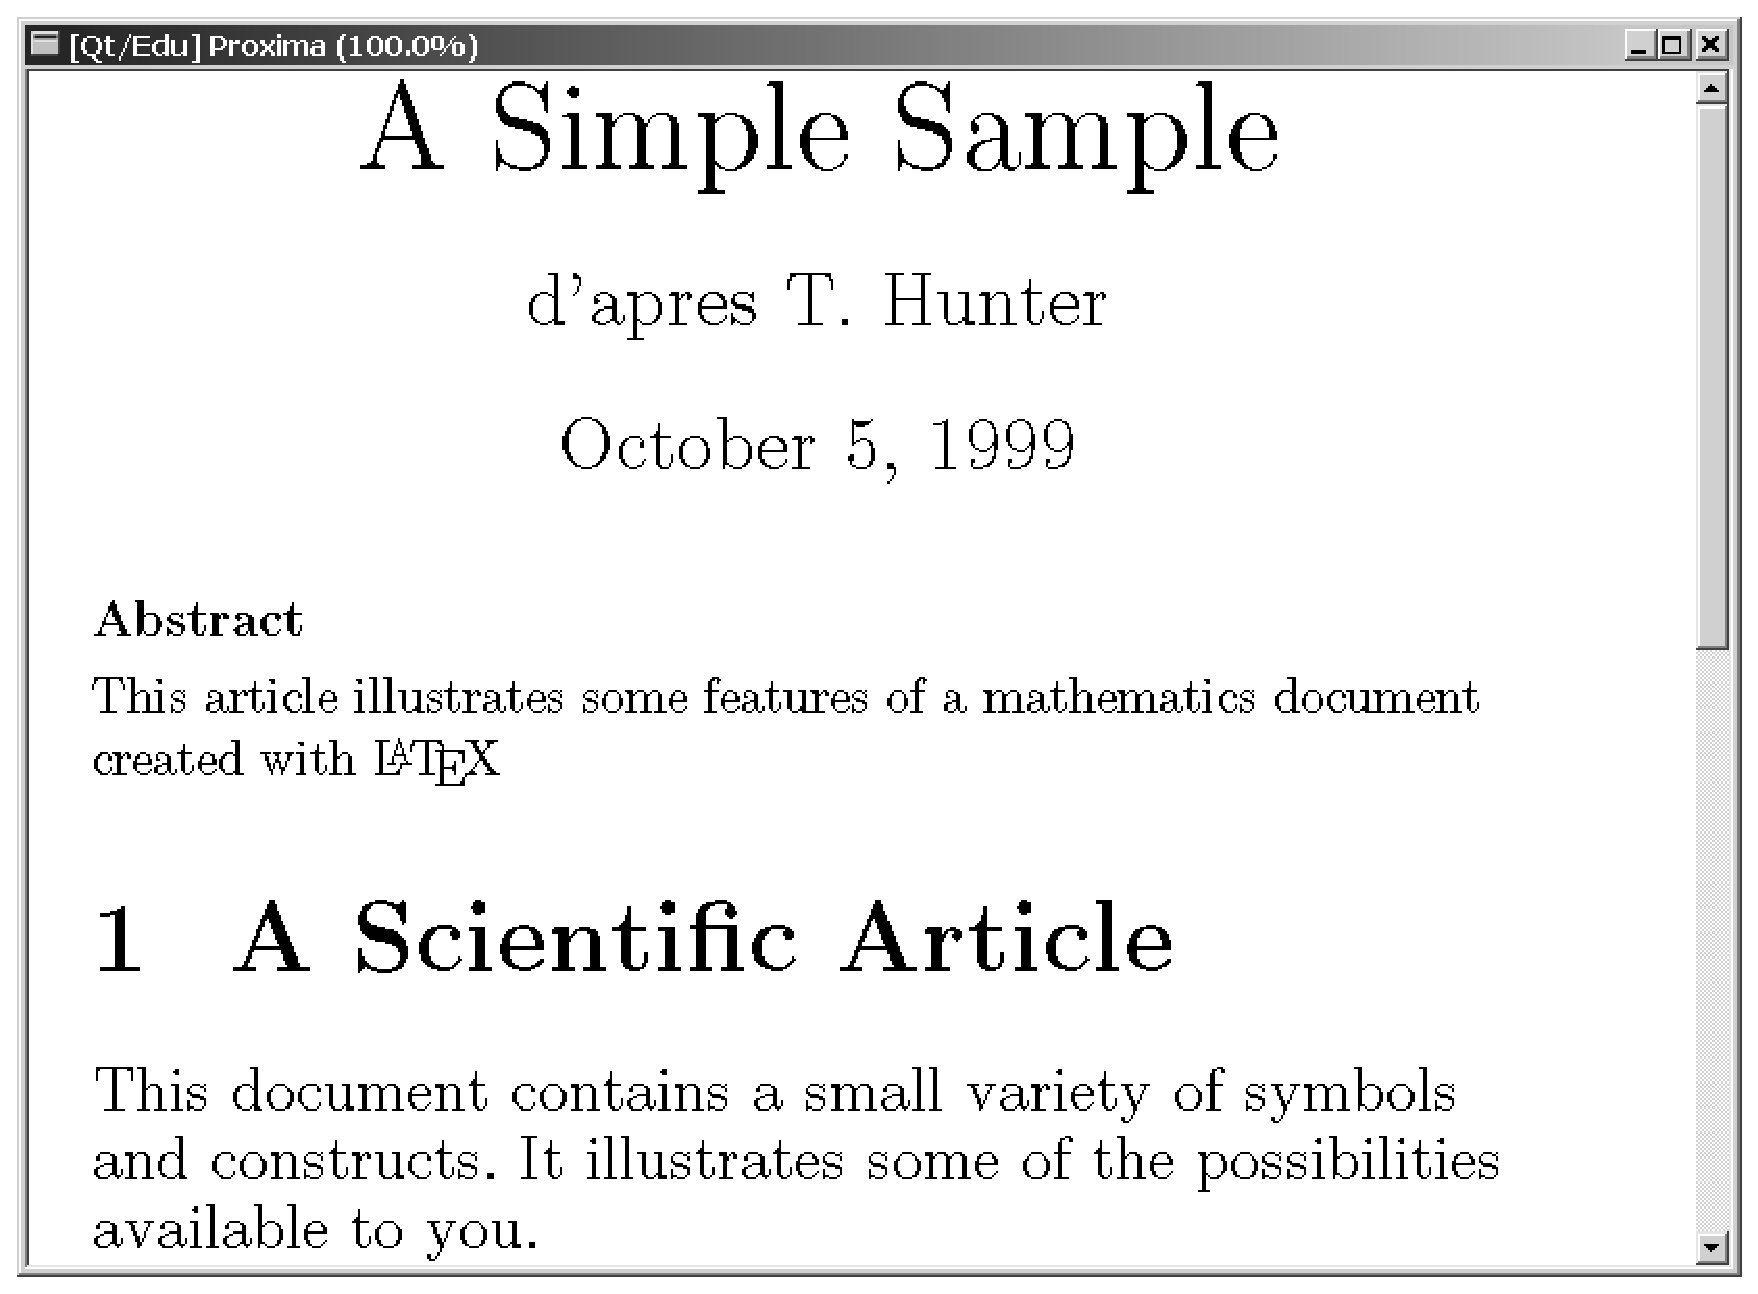
\epsfig{file=xprezpics/eps/xlatex1.png.eps, width=2in} \qquad
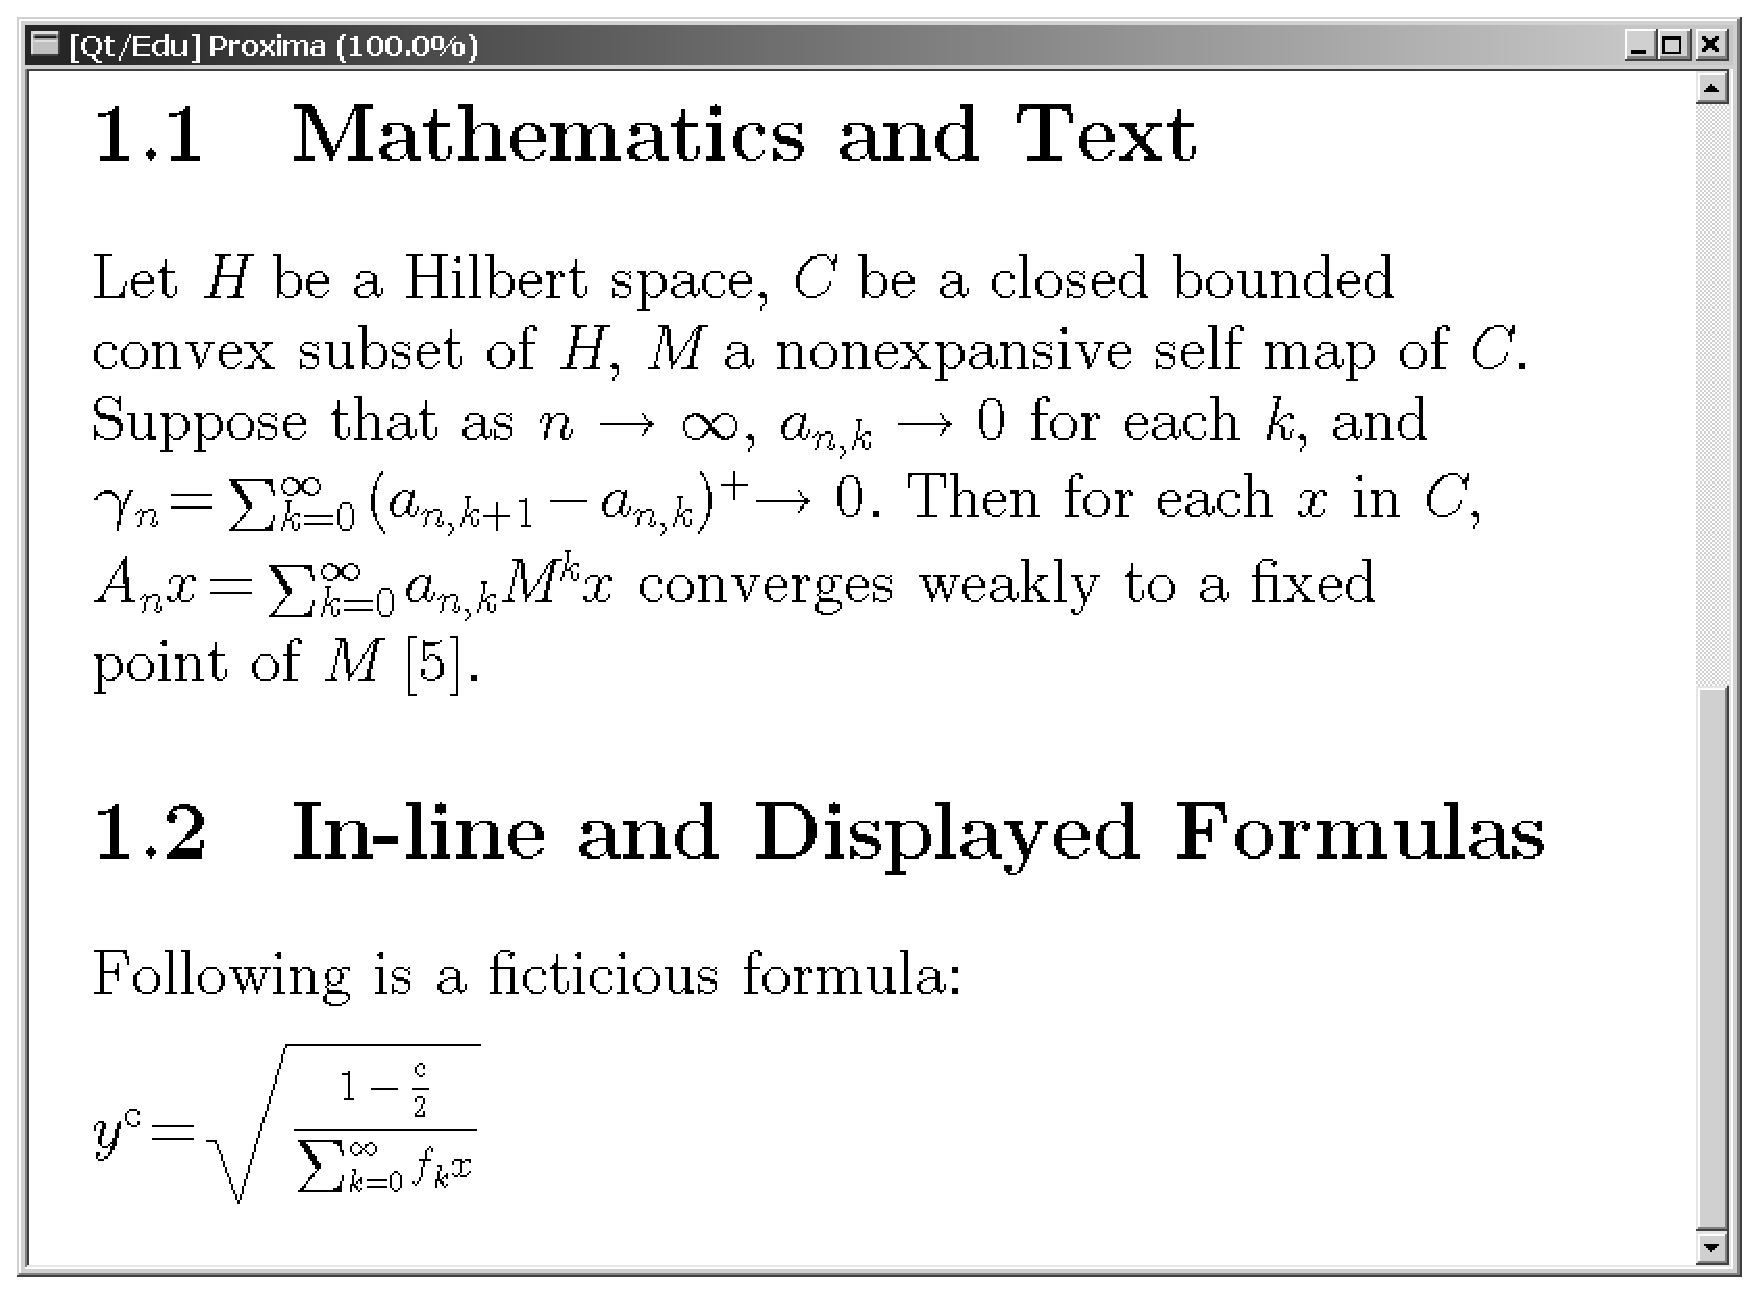
\epsfig{file=xprezpics/eps/xlatex2.png.eps, width=2in}
\end{center}
\par The contributions of this paper are:
 \begin{itemize}
 
 \item An evaluation of the strengths and weaknesses of existing
        presentation languages, resulting in a list of requirements for a presentation
        language.
 \item A proposal for the declarative presentation language {\sc Xprez}
        that supports both the flow and the box model, has presentations as first-class
        objects, and has a powerful abstraction mechanism.
 \end{itemize}

\par Two kinds of languages are involved in the presentation process: a
      presentation target language, and a presentation specification or
      transformation language. The presentation target language describes the
      building blocks of the presentation that is shown on the screen or sent to a
      printer, whereas the transformation language describes how an XML document is
      mapped onto the target language to create this presentation. The Extensible
      Stylesheet Language (XSL) gives a clear example of the distinction, as it has
      been split into a transformation language (XSL Transformations or XSLT) and a
      target language (XSL Formatting Objects). XSLT documents specify
      transformations that map a source document tree to a tree of Formatting
      Objects, which can then be rendered. 
\par Section~\ref{targetlangs} discusses existing presentation
      target languages, followed by the introduction of the target language of
      {\sc Xprez} in Sect.~\ref{xpreztarget}. Section~\ref{transformlangs} deals with the transformation languages and
      Sect.~\ref{conclusions} concludes.
\section{Presentation Target Languages}
\label{targetlangs}
\par The elementary building blocks of most presentation target languages are
      basic presentations of strings and small graphical objects such as lines,
      squares and circles. They can be composed according to a number of models:
 \begin{description}
 
 \item[Flow model]
When a flow model is used, presentations are placed next to each
        other or above each other, depending on the current flow direction. If the
        remaining space in the current direction is too small to fit the presentation,
        a new flow presentation is started. In this way, lists of words can be divided
        into lines and lists of lines can be divided into pages. The generated list of
        flows may then be manipulated further, for example, by extending each page in a
        list of pages with a header and a footer.
 \item[Box model]
The box model allows each presentation to define its position
        relative to sibling or parent presentations. The positions can be set either
        directly by specifying them relative to positions of other presentations, or by
        declaring constraints. If constraints are used, the style sheet does not so
        much specify the exact calculation of a property, but rather gives constraints
        that should hold for the property. The actual computation of the property value
        is left to a constraint solver. 
 \item[Matrix model]
The matrix model can be used to align a tree of cells, usually a list
        of rows that each contain a list of cells, along the rows as well as the
        columns. This is difficult to specify just using rules for each row and cell,
        as the width of the n-th cell has to be related to the n-th cells in the other
        rows instead of to properties of its parent or sibling cells. Matrices can be
        used to create box presentations, but the extent to which this is possible
        depends on the expressivity of the matrix model; for example, whether or not
        cells may overlap.
 \item[Absolute positioning]
A very low level way of formatting is specifying the absolute
        coordinates in the resulting presentation.
 \end{description}

\subsection{Existing Presentation Target Languages}
\label{existingtarget}
\par In this section, we will examine the target sublanguages of five
        presentation languages: CSS~2.0, CCSS, XSL, PSL and P. Of these five
        languages, only XSL regards its target language as a separate language with its
        own syntax. The other languages only describe how properties of the elements of
        the target presentation tree can be set, but they do not treat presentations as
        actual values in the language.
\par \bigskip{\bf CSS~2.0:} Cascading Style Sheets,
        level~2~\cite{css} is an example of a simple presentation
        language. Its target language is almost invisible to the style sheet designer.
        The presentation of a document is a tree that is almost isomorphic to document
        tree, with the document content in the leaves. It is not entirely isomorphic,
        because content can be left out and simple text content can be added. The nodes
        of the tree specify presentation properties such as font size or color, either
        absolutely or as a percentage, but arbitrary expressions are not allowed. The
        kind of a property determines to what property a percentage refers. For
        instance, a percentage value for the {\em font-size} property refers to the
        font size of the parent element, but a percentage for the {\em line-height}
        property refers to the font size of the element itself. It is not possible to
        let a property value depend on arbitrary properties of the parent or siblings
        in the presentation tree. CSS~2.0 supports a flow layout and absolute
        positioning. There is also a table format, but it is of limited use because the
        transformation language is rather weak. Consequently, if the data in the
        document does not have exactly the same structure as a CSS~2.0 table, it
        cannot be presented as one.
\par \bigskip{\bf CCSS:} Constraint Cascading Style
        Sheets~\cite{ccss} is an extension of the CSS~2.0 standard
        that is based on constraints. CCSS's target language closely resembles the
        CSS~2.0 target language, but child properties are specified using
        constraints instead of percentages of the parent's property values. Another
        difference is that the constraints can refer to global constraint variables and
        to left-siblings in the presentation tree as well as to the parent node. 
\par \bigskip{\bf XSL FO:} On the other side of the spectrum is
        the XSL language. The target language, XSL Formatting Objects, consists of a
        large collection of elements that can be used to specify page models,
        presentation properties, and more complicated presentation aspects, such as
        hyphenation and counters. A presentation is a tree that consists of these
        formatting objects. The style sheet offers strong control over the flow model,
        but no box model is supported. There is a table model, but using it to do a box
        layout is difficult, because the style sheet would then have to take care of
        the alignment, and XSLT does not support a strong computational formalism.
\par \bigskip{\bf PSL:} The Proteus Stylesheet
        Language~\cite{psl} is an attempt to combine the simplicity of
        CSS~2.0 with the power of XSL. Its target language is again close to the
        CSS target language. PSL extends the CSS target language with a box model and
        graphical symbols. The value of a property can be expressed as a mathematical
        expression that refers to properties of nodes in the presentation tree. This
        mechanism is called {\em property propagation}. PSL supports a constraint
        based box model. Presentations can specify their position and size properties
        relative to other presentations in the tree, which are addressed using a number
        of primitive functions for accessing siblings, parents and ancestors of a
        specified type, etc.
\par \bigskip{\bf P:} The last language considered here is the
        presentation language P of the Thot editor toolkit~\cite{thot}.
        It has a target language that consists entirely of boxes. Instead of having a
        large number of different presentation boxes, like the XSL Formatting Objects,
        P has only three kinds of boxes with a large number of properties. In contrast
        to PSL, the box layout in P is not constraint based, so the style sheet
        designer needs to take the order of computation of the layout properties into
        account. P does support horizontal and vertical reference lines for automatic
        alignment of boxes. Matrices are not primitive objects in P.
\par \bigskip{\bf Discussion:} The languages discussed above are
        all declarative and domain-specific languages that vary in expressive power.
        The simple languages CSS~2.0, CCSS, and PSL allow simple presentations to
        be specified in a simple way, but cannot be used to specify more complex
        presentations, such as mathematical formulas. In contrast, XSL and P do allow
        complex presentations to be specified, but due to the lack of abstraction,
        simple presentations also have rather elaborate specifications, especially in
        P. 
\par Only P and PSL support a box model, but both models are of a rather
        object-oriented and imperative nature. A box can specify its own position
        properties relative to its parent or siblings, but it is not possible to state
        at parent level that two child presentations should have their top and bottom
        aligned, or that two presentations should have the same width. As a
        consequence, a conceptually simple change of presenting the children of a node
        next to each other instead of above each other, requires changing the
        presentations for all child elements. Moreover, if the choice for vertical or
        horizontal layout depends on an attribute of the parent, then all children
        require code in their presentation rules for accessing this parent attribute,
        if possible, and letting their presentation depend on its value. If, however,
        presentations are first-class objects in the target language, then the parent
        presentation rule can specify the layout of the children.
\par Letting a child presentation specify its own layout makes it more
        difficult to understand a presentation. For example, a reverse order
        presentation of a list of children is obtained by aligning each right side with
        the previous child's left side. If, on the other hand, child presentations are
        first-class, and abstraction mechanisms can be used to define combinators on
        them, reversing can be specified by a simple reverse combinator. Another
        advantage of this approach is that the concepts of reversing and direction of
        layout are orthogonal now. Changing the layout from a horizontal list to a
        vertical list can be achieved by applying a different combinator to the
        reversed children, while the order of the children is controlled by applying
        the reverse combinator or not. In the P and PSL model, these concepts are
        intertwined.
\par \bigskip{\bf  Requirements:} Based on the previous
        discussion, we can conclude that a presentation target language, and in
        particular the target language for Proxima, will have to meet the following
        requirements: 
 \begin{description}
 
 \item[Proportional effort]
 It must be possible to specify complex presentations, but the
          specification of simple presentations should still be easy.
 \item[Declarative]
In a declarative language, understanding a composite presentation
          is easier, because the computation of a presentation does not generate side
          effects. Another advantage is that the designer does not need to worry about
          the order of computation of presentations and properties.
 \item[Domain-specific]
 The language should have syntax for presentation specific
          constructs such as an {\bf em} (height of the letter m in the current font and
          size) and different measuring units such as pixels and inches.
 \item[Flow and Box model with alignment]
The language requires a flow model for textual parts of a
          presentation, and a box model for displaying mathematical formulas and other
          more graphical presentations such as trees. Automatic alignment is required in
          order to be able to specify composite presentations without having to
          explicitly position each child presentation.
 \item[First-class presentations]
A first-class presentation can be named and manipulated at the
          level of its parent, which in many cases is the natural place to manipulate it.
          At the same time, it is still possible to specify properties at child
          presentation level, when this is more appropriate.
 \item[Powerful abstraction mechanism]
User-defined functions and var\-i\-ables help to reduce code
          duplication, facilitate code reuse, and increase transparency, because
          complicated pieces of code may be replaced by functions with well-chosen
          names.
 \end{description}

\section{The {\sc Xprez} Target Language}
\label{xpreztarget}
\par With the requirements from the previous subsection in mind, we have
      developed the declarative presentation language {\sc Xprez}. 
\subsection{{\sc Xprez} Presentation Model}

\par {\sc Xprez} is a box language, like P, and the document formatting
        languages \TeX ~and Lout~\cite{lout}. A presentation is a value of the abstract data type
        \texttt{Xprez}, the definition of which is omitted. A presentation is either a
        simple box containing a piece of text or a graphical object, or a composite box
        that contains a list of child presentation boxes. It can therefore be viewed as
        a tree in which the leaves are simple presentations and the nodes are composite
        presentations. We construct \texttt{Xprez} values in the functional language
        Haskell extended with a number of primitive functions that will be described in
        Sect.~\ref{primitives}.
\begin{figure}
\begin{small}
\begin{center}
\begin{small}\begin{verbatim}data Inh = Inh {fontFamily :: String, fontSize :: Int,
                textColor, lineColor, fillColor, backgroundColor :: Color} 
data Syn = Syn {hRef, vRef, minWidth, minHeight :: Int,
                hStretch, vStretch :: Bool}\end{verbatim}\end{small}
\caption{The {\sc Xprez} properties}\label{xprezproperties} 
\end{center}
\end{small}
\end{figure}
\pagebreak
\par A presentation box (from now on called presentation) has a number of
        properties that describe its size and its appearance: \begin{center}
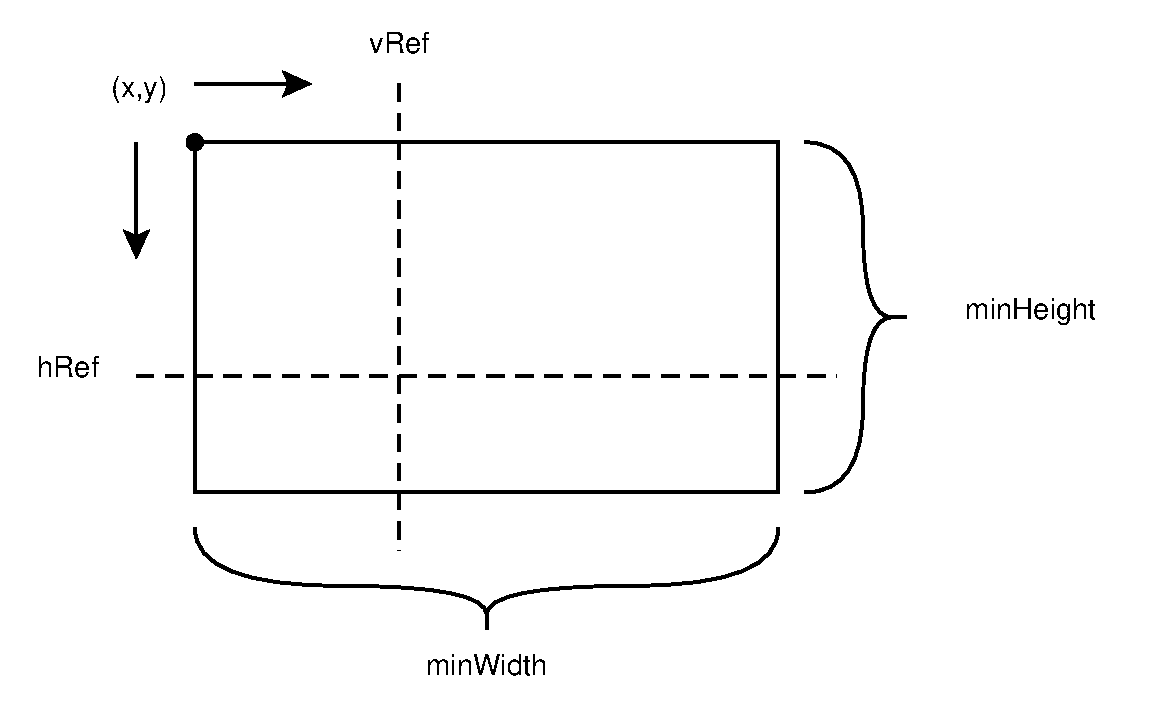
\epsfig{file=xprezpics/eps/picob.eps, width=2in}
\end{center}
\par \noindent Figure~\ref{xprezproperties} contains
        the definition of the two records \texttt{Inh} and \texttt{Syn} (as explained
        below) with the type of each of the properties. The \texttt{hRef} and
        \texttt{vRef} properties specify the horizontal and vertical reference lines
        that are used for aligning boxes when they are combined in composite
        presentations. The boolean properties \texttt{hStretch} and \texttt{vStretch}
        specify whether or not the presentation is allowed to stretch in horizontal or
        vertical direction. The rest of the properties are \texttt{fontFamily},
        \texttt{fontSize}, \texttt{textColor}, \texttt{lineColor}, \texttt{fillColor},
        and \texttt{backgroundColor}, which should be self explanitory. In the future,
        this set will be extended with other properties such as more line style and
        font attributes, and user defined properties will be supported. The
        presentation tree is transformed into an attribute grammar in which the font,
        style, and color properties are inherited attributes that go down in the tree,
        and alignment and stretch properties are synthesized attributes that go up in
        the tree. In the Haskell types, this division is visible in the fact that the
        properties are modeled using two records: \texttt{Inh} for inherited
        properties, and \texttt{Syn} for synthesized properties.
\subsection{{\sc Xprez} Primitives}
\label{primitives}
\par Simple presentations can be created with the first five combinators in
        Fig.~\ref{xprezprim}. The \texttt{empty} combinator is a neutral
        element that is not visible and takes up no space. A piece of text can be
        presented with \texttt{text}, and a rectangle with \texttt{rect}, which takes
        the width and height as arguments. The \texttt{poly} combinator takes a list of
        relative coordinates between (0,0) and (1,1) and produces a line figure that
        connects these points. A \texttt{poly} presentation stretches in horizontal and
        vertical direction. Finally, \texttt{img} can be used to display bitmap images.
        The argument is a string that contains the path to the bitmap file. By default,
        the reference lines of simple presentations are 0, except for the horizontal
        reference line of a text presentation, which is equal to the baseline of the
        current font.
\begin{figure}
\begin{small}
\begin{center}
\begin{small}\begin{verbatim}empty             :: Xprez
text              :: String -> Xprez             -- simple text
rect              :: Int -> Int -> Xprez         -- rectangle
img               :: String -> Xprez             -- image (jpg, png, ...)
poly              :: [ (Float, Float) ] -> Xprez -- poly line
row, col, overlay :: [ Xprez ] -> Xprez          -- row, column, overlay
rowR, colR        :: Int -> [ Xprez ] -> Xprez   -- row, col w/ reference
matrix            :: [[ Xprez ]] -> Xprez
format            :: [ Xprez ] -> Xprez\end{verbatim}\end{small}
\caption{The {\sc Xprez} primitives}\label{xprezprim} 
\end{center}
\end{small}
\end{figure}

\par There are several kinds of composite presentations, the simplest being
        rows and columns (combinators \texttt{row} and \texttt{col}), which are duals.
        In a row, each child presentation is placed immediately to the right of its
        predecessor, with their horizontal reference lines aligned. Vertical reference
        lines have no effect on the positioning in a row. \begin{center}
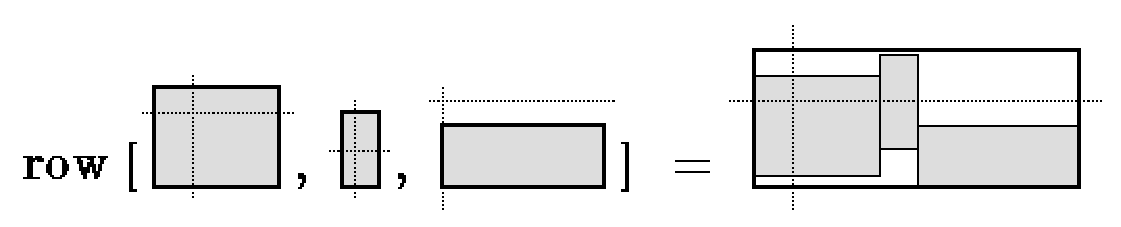
\epsfig{file=xprezpics/eps/row.png.eps, width=2.5in}
\end{center}
\par \noindent The bounding box of a row is the smallest rectangle
        that encloses all its children. The horizontal reference line is equal to the
        aligned reference lines of the children, whereas the vertical reference line is
        taken from one of the children (by default the first one). The \texttt{rowR}
        combinator takes an extra argument of type \texttt{Int} that specifies which
        child carries the vertical reference line for the row. \texttt{}By default, a
        row stretches in horizontal direction if one of its children does, and it
        stretches in vertical direction if all children stretch vertically. However, by
        setting the stretch properties, these defaults can be overridden. 
\par  The \texttt{matrix} combinator can be used to describe a table
        layout, in which elements are aligned with elements to their left and right as
        well as with elements above and below them. 
\par Because \texttt{row}, \texttt{column} and \texttt{matrix} do not allow
        their children to overlap, a special combinator is required to create
        overlapping presentations. The \texttt{overlay} combinator places its children
        in front of each other, while aligning both the horizontal and vertical
        reference lines. It can be used to create underlined text, for example. Because
        alignment takes place on both reference lines and hence all child reference
        lines overlap, no special \texttt{overlayR} combinator is needed. 
\par The last composite combinator in Fig.~\ref{xprezprim}
        is \texttt{format}. It takes list of presentations as argument and splits this
        list into rows based on the available horizontal space. The resulting rows are
        placed in a column. The \texttt{format} combinator can be used to display a
        paragraph of words, or any other kind of presentations for that matter, on a
        number of lines. 
\par Here is an example {\sc Xprez} presentation that illustrates
        alignment and stretching in a row:\begin{small}\begin{verbatim}let cross     = poly [(0,0),(1,0),(1,1),(0,1),(0,0),(1,1),(0,1),(1,0)]
    greycross = cross `withbgColor` grey
in  row [ text "Big" `withFontSize` 200
        , colR 2 [ cross, cross, text "small", greycross, greycross ] ] \end{verbatim}\end{small}

\par \noindent This produces the following image (the dashed line has
        been added and represents the horizontal reference line of the
        presentation):\begin{center}

\epsfig{file=xprezpics/eps/align.png.eps, width=1in}
\end{center}
\par The second element in the row is a column that takes the horizontal
        reference line from its third child (the numbering starts at 0), so the word
        {\bf ``Big''}, displayed with a font size of 200 pixels, is aligned with the
        word {\bf ``small''}, which has the default font size. The \texttt{cross}
        object is a line figure in the form of an X, and the \texttt{greycross} is that
        same figure with a grey background color. Because these presentations stretch
        in vertical direction, so does the column that contains them. The two
        stretching objects above the reference object (\texttt{text "small"}) are each
        assigned equal amounts of the remaining space above the horizontal reference
        line, and likewise, the objects underneath the reference object are assigned
        the remaining space below the reference line. If, on the other hand, the
        reference object itself is allowed to stretch, then the total amount of
        available space is added and distributed equally over all stretching objects.
        In this case, there will no longer be any alignment of the reference object.
        
\subsection{Property Modification}

\par The properties of a presentation can be modified using the generic
        \texttt{with\symbol{95}}\footnote{The name contains an underscore because Haskell
        already has a keyword {\em with}} combinator:\begin{small}\begin{verbatim}with_ :: Xprez -> ((Inh, Syn) -> (Inh, Syn)) -> Xprez\end{verbatim}\end{small}

\par  In the specification of a property value, the original values of
        properties can be used, e.g. the font size can be set to the old font size
        increased with 2 points. Therefore, the second argument of \texttt{with\symbol{95}}
        is a function that takes the original values of the inherited attributes that
        come from the parent and the synthesized attributes that come from child
        presentation as arguments, and returns the new values (i.e. the inherited
        attributes that go to the child and the synthesized attributes that go to the
        parent).
\par  The inherited and synthesized property values are Haskell records,
        which have special syntax for accessing and updating fields. If \texttt{inh} is
        a value of type \texttt{Inh}, then the expression \texttt{fontSize inh} denotes
        the value of the fontSize field in \texttt{inh}, and \texttt{inh $\{$ fontSize =
        10 $\}$} denotes a value of type \texttt{Inh} in which all fields have the
        same values as in \texttt{inh}, except for the \texttt{fontSize} field, which
        is now 10. Below is the definition for the \texttt{withFontSize} combinator:
        \begin{small}\begin{verbatim}withFontSize :: Xprez -> Int -> Xprez
withFontSize xp fs = xp `with_` \(inh, syn) -> (inh {fontSize = fs}, syn)\end{verbatim}\end{small}

\par Constructing functions comes with some syntactic overhead, but by
        using a libary of combinators for the most frequent uses, most of the calls to
        the actual \texttt{with\symbol{95}} combinator can be avoided. However, a problem
        with this derived combinator is that is that the \texttt{fs} value is of type
        \texttt{Int}, and therefore cannot depend on the original font size value. A
        different combinator that takes a function of type \texttt{Int -> Int} as
        argument, which is used in the fraction example below, solves this problem:\begin{small}\begin{verbatim}withFontSize_ :: Xprez -> (Int -> Int) -> Xprez
withFontSize_ xp ffs = 
  xp `with_` \(inh, syn) -> (inh { fontSize = ffs (fontSize inh) }, syn)\end{verbatim}\end{small}

\par With \texttt{p `withFontSize\symbol{95}` (\symbol{92}fs -> 2*fs)} we can now
        specify the doubling of the font size for a presentation \texttt{p}, but again,
        this requires a function in the presentation code, although it is easier to
        write than the functions required by \texttt{with\symbol{95}}. A more natural
        solution is the declaration of a special data type \texttt{Length}, with
        operations such as addition and multiplication, but which also has primitive
        values that represent current font properties. In Haskell, type classes can be
        used to accomplish this. Using type classes, it will be possible to write:
        \linebreak \texttt{hSpace (2*em)}, which denotes a horizontal space of twice
        the height of the letter m in the current font. A future version of
        {\sc Xprez} will support special syntax for \texttt{with\symbol{95}}, so \texttt{text
        "a" with $\{$ child.fontSize = parent.fontSize * 2 $\}$} can be written
        without explicit functions.
\par The font size combinators show how abstraction is used to meet the
        {\em proportional effort} requirement. For simple changes of the font size,
        the simple \texttt{withFontSize} combinator can be used, and only if more
        control is desired, it is necessary to use the more complicated
        \texttt{withFontSize\symbol{95}} or \texttt{with\symbol{95}} combinators.
\subsection{Advanced Examples}

\par A presentation in {\sc Xprez} is a first class value, so it is
        possible to perform manipulations on child presentations, such as positioning
        or font size updates, at parent level. This is illustrated in the following
        presentation for mathematical fractions: \begin{small}\begin{verbatim}frac e1 e2 = let numerator   = hAlignCenter (pad (shrink e1) )
                 bar         = hLine
                 denominator = hAlignCenter (pad (shrink e2) )
             in  colR 2 [ numerator, vSpace 2, bar
                        , vSpace 2, denominator ] `withHStretch` False

pad xp = row [ hSpace 2, xp, hSpace 2 ]
                 
shrink e = e `withFontSize_` (\fs -> (70 `percent` fs) `max` 10)\end{verbatim}\end{small}

\par \noindent The non-primitive library function
        \texttt{hAlignCenter}, centers its argument horizontally, and the
        \texttt{shrink} function reduces the font size to 70\%, with a minimum of
        10. The result of \texttt{(text "x" `frac` text "2") `frac` text "1 + y"}
        is:\begin{center}
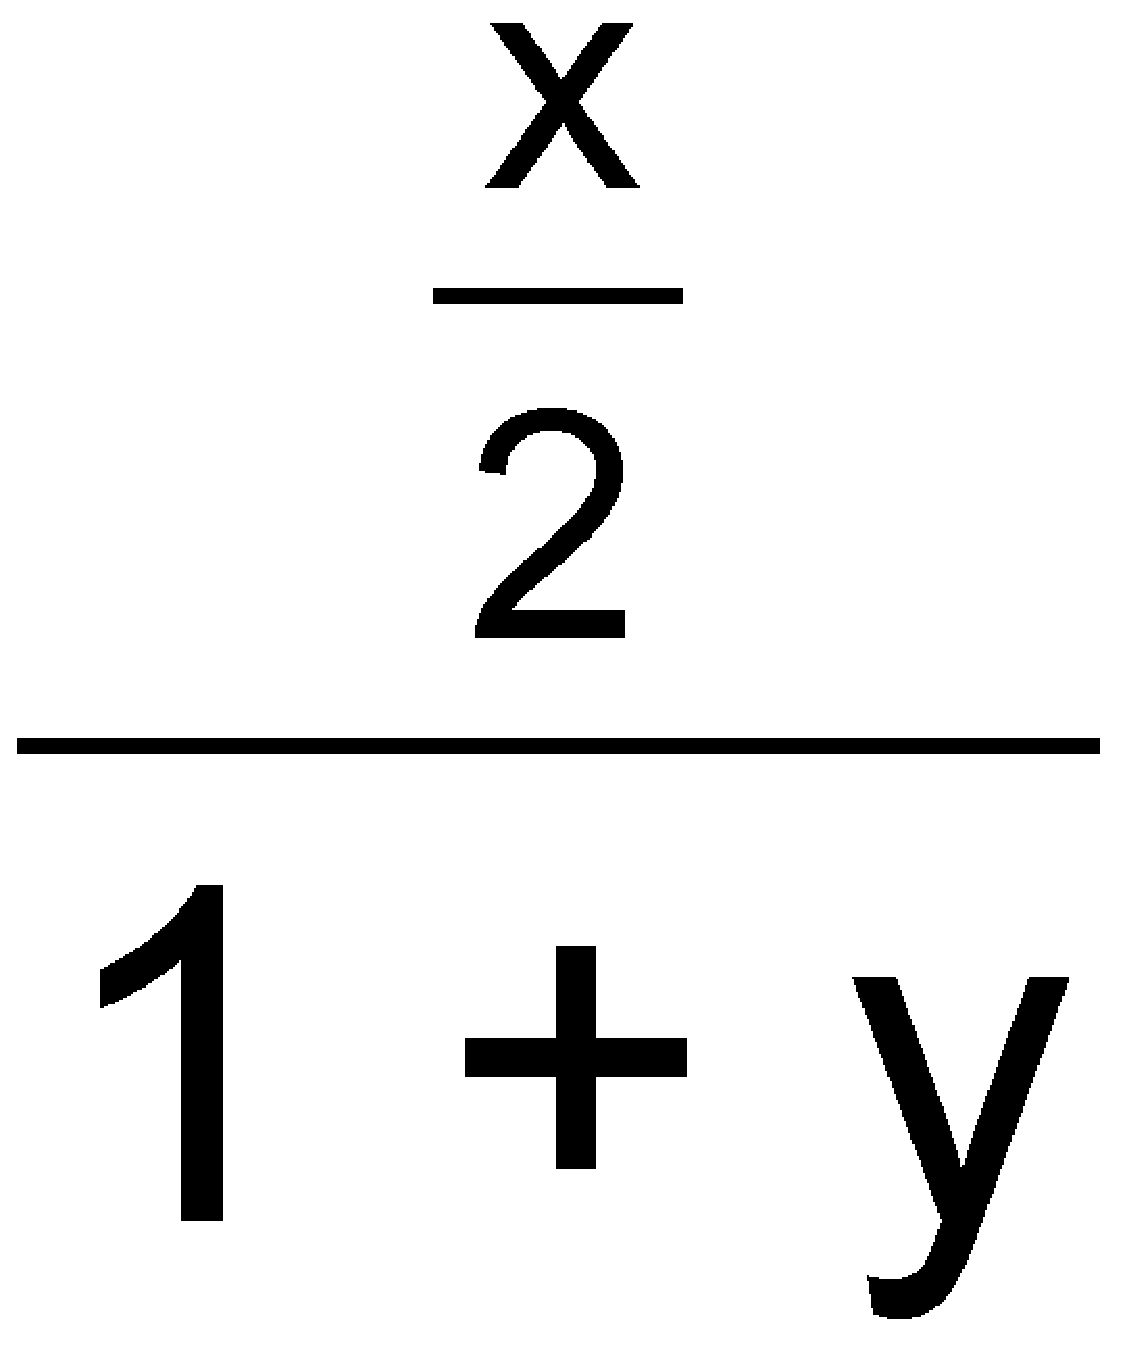
\epsfig{file=xprezpics/eps/frac.png.eps, width=0.5in}
\end{center}
\par The \texttt{pad} and \texttt{shrink} functions illustrate the
        {\em first-class} and {\em abstraction} requirements. Because a
        presentation is a first-class values, the presentations of the numerator and
        the denominator can be addressed and manipulated in the presentation of the
        fraction. Furthermore, using abstraction, the manipulations can be captured in
        the functions \texttt{pad} and \texttt{shrink}. In contrast, child
        presentations in both P or PSL cannot be addressed at parent level, so the
        fraction presentation must be created by letting each child, including the
        fraction bar specify its appearance and relative position. As a result, it is
        difficult to reuse parts of a presentation in another presentation, since all
        parts refer to each other, and the manipulations on the appearance are harder
        to read, because no abstraction can be used. 
\par The second example is a pair of combinators that can be used to create
        tree browser presentations:\begin{center}
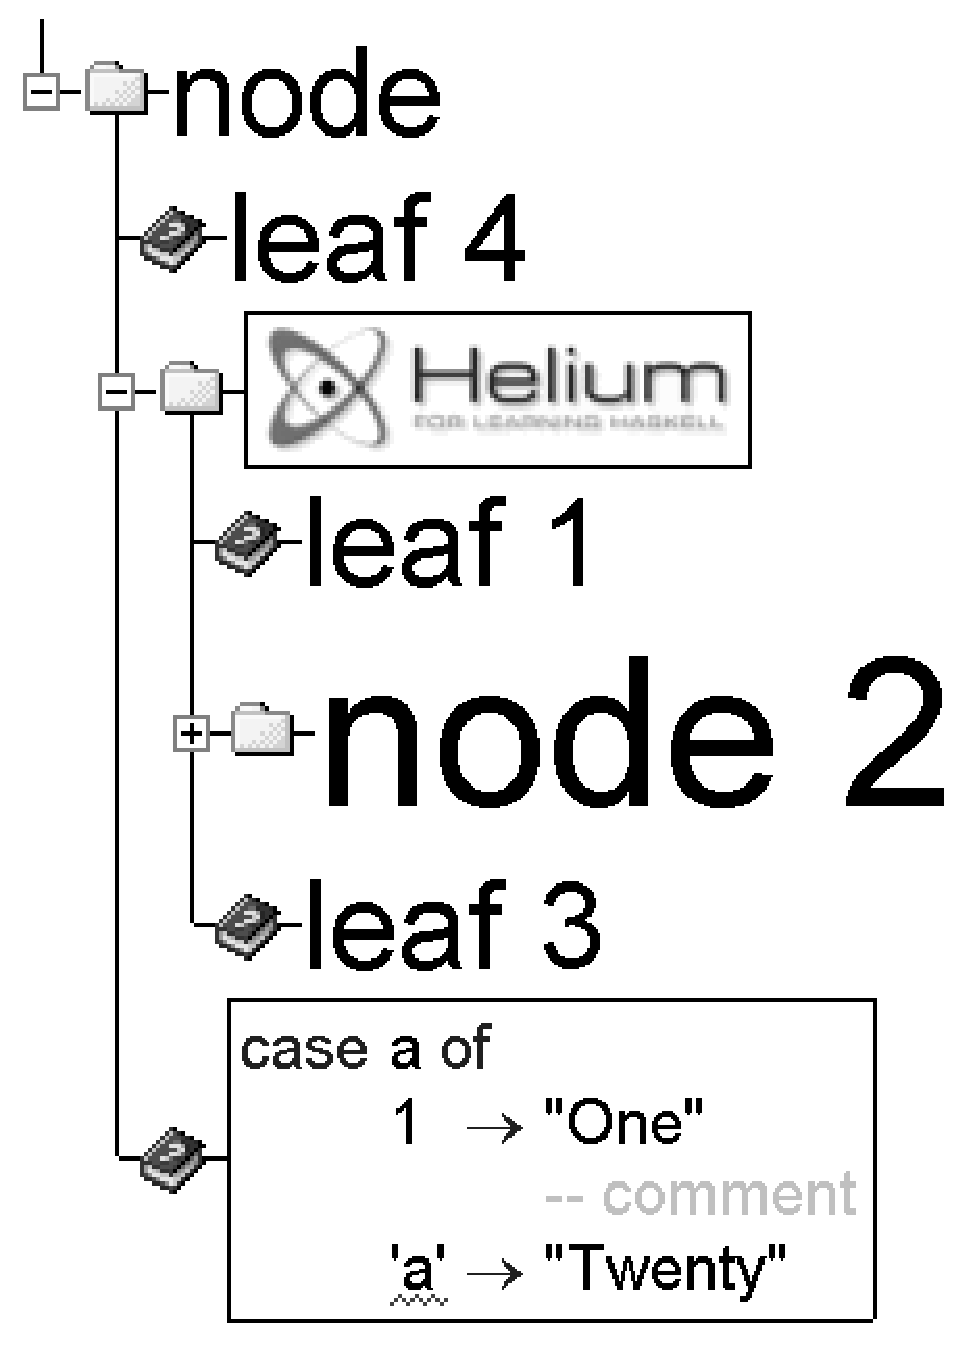
\epsfig{file=xprezpics/eps/tree.png.eps, width=1in}
\end{center}
\par \noindent This image has been created with the
        \texttt{mkTreeLeaf} and \texttt{mkTreeNode} combinators, which are defined in
        20 lines of {\sc Xprez} code (see the Appendix for the source). Both
        combinators take an \texttt{Xprez} argument that is the presentation of the
        label, and the tree node also takes a list of child presentations (which should
        be either nodes or leaves for a correct tree, but can actually be any value of
        type \texttt{Xprez}). Labels are not restricted to text, but can also be
        images, or composite {\sc Xprez} presentations, like the label that contains
        the case expression in the last leaf of the example tree. 
\par The tree example is given here to show that a rather complex and
        graphical presentation can be specified with relatively little effort. However,
        in order to make this presentation a fully operational tree browser that can
        react to mouse clicks, we need to model the presentation state and edit
        operations on this state. This is not possible in the current version of
        {\sc Xprez} but will be possible in the Proxima editor system.
\subsection{Future Work}

\par {\sc Xprez} meets the requirements listed at the bottom of
        Sect.~\ref{existingtarget}, with the exception of the
        domain-specific syntax, for which a special parser will have to be added to the
        system. Furthermore, there are a number of things that are still lacking in the
        current model and that are being investigated. Firstly, there is no page model
        yet, and hence no page related concepts such as footnotes and page references
        are possible. Probably, an abstraction similar to the {\em Galley} from
        Lout~\cite{lout} can be used for this. Secondly, there is no
        primitive notion of padding, which will allow spacing in columns and rows to be
        specified more naturally. Both of these concepts are related to the need for a
        more powerful \texttt{format} primitive that can handle both horizontal and
        vertical formatting while offering more control over the generated rows and
        columns. Finally, the \texttt{with\symbol{95}} combinator only gives access to the
        properties of a parent and its child. It is not possible to access properties
        of siblings, or presentations elsewhere in the tree, but it is also not yet
        clear whether such access is really necessary in a presentation language.
        Nevertheless, the set of combinators presented so far is powerful enough to
        cover much of the \TeX ~math typesetting as described in
        \cite{functionaltex}, including superscripts and subscripts. We also
        expect that defining a presentation sheet for the MathML~\cite{mathml} language will be rather straightforward in {\sc Xprez}.
\section{Presentation Transformation Languages}
\label{transformlangs}
\par A presentation transformation language is used to specify a mapping
      between a document language (a subset of XML defined by a DTD) and a
      presentation target language. It may be a complete programming language, which
      is powerful, but leaves the burden of traversing the document structure on the
      programmer. Therefore, often a rule based language is used. For each element in
      the document type, one or more rules can be specified, which map the element
      onto its presentation. 
\subsection{Existing Languages}

\par The five languages discussed in Section~\ref{targetlangs} all have rule-based transformation languages. However,
        the power of the rule selection mechanisms varies, as well as the
        transformation capabilities.{\bf }
\par {\bf CSS~2.0:} In CSS~2.0, rules are used to specify the
        appearance of elements or classes of elements. These rules are either applied
        to certain types of elements (e.g. all \texttt{Title} elements in the
        document), or depend on contextual information of an element (e.g. all elements
        that are a child of a \texttt{Section} element). The body of a rule consists
        just of property declarations.
\par It is possible to leave out the presentation of certain elements, and
        to add textual content before or after a presentation element in CSS~2.0,
        but general tree transformations cannot be specified. It is also not possible
        to specify computations. Therefore, a more complicated presentation structure,
        such as a table of contents or a section reference is impossible to specify
        using CSS~2.0. Frequently used derived values, such as element counters,
        have been added as primitives to the language, but they are not very flexible.
        Furthermore, the addition of special cases instead of a general solution,
        increases the complexity of the semantics of the language.
\par \bigskip{\bf CCSS:} The constraint mechanism of CCSS offers a
        more flexible rule selection. If the presentation environment differs from the
        one the designer had in mind, causing rules to fail, constraints can still
        specify an acceptable presentation, because they degrade continuously instead
        of discreetly. In CSS~2.0, a rule either succeeds or fails, but does not
        say anything about an approximate solution, leaving the choice to the rendering
        agent instead of to the style sheet designer. As a concrete example, it is
        possible to specify with constraints that no fonts should be smaller than 11
        points, but if the actual font is at least 11 points, then this actual size
        should be chosen. Finally, CCSS also allows the specification of global
        constraints. For example all tables can be constrained to have the same width,
        without actually specifying this width.
\par \bigskip{\bf XSLT:} XSLT has a more powerful rule selection
        mechanism than the other languages discussed here. Specifying a rule to apply
        only to an element that is the second child of its parent, for example, is
        possible in XSLT but not in the other languages. XSLT supports conditional
        processing with if and case expressions based on document content or attribute
        values. However, the most important difference with the other languages is the
        fact that the resulting transformed tree need not be isomorphic to the document
        tree. The style sheet can direct the transformation process, supporting
        multiple passes over the document tree and allowing full structural
        transformations of the document. Unfortunately, XSLT does not allow the
        application of the style sheet to generated parts of the tree. This means that
        derived structures must be specified directly in the target language, whereas
        it would be more elegant to specify them in terms of the document language. In
        other words, it is not possible to specify derived document parts using logical
        markup instead of physical markup, as the former one would require another
        transformation pass over the generated tree.
\par \bigskip{\bf PSL:} The transformational capabilities of PSL
        are slightly weak\-er than those of XSLT, because the only way to influence the
        resulting tree is by extending the presentation tree with so called tree
        elaborations. Reversing a list of children is not possible in general, but can
        be simulated by having each child presentation put itself in front of the
        presentation of its predecessor. However, the resulting tree follows the
        structure of the original document tree, and a table of contents, for example,
        which requires a double pass over the document tree, cannot be specified
        elegantly in PSL.
\par \bigskip{\bf P:} In P, each element type has only one rule.
        An element presentation that depends on contextual information can be specified
        using conditionals that depend on the document structure. So instead of having
        a special rule for each possible parent an element may have, there is only one
        rule that alters its behavior based on the elements parent. A conditional
        presentation may also be based on a number of other factors, including document
        attributes and counter values, but no general boolean expressions are allowed.
        An important difference between P and the other presentation languages is that
        several views can be explicitly defined in the style sheet. 
\par \bigskip{\bf Discussion:} None of the discussed presentation
        languages have good support for abstraction. Only XSLT allows the definition of
        functions and variables, but these come at a high syntactic overhead, and no
        higher-order functions can be defined. As a result, a style sheet for a larger
        document type in which many elements have a similar presentation, becomes
        cluttered with a large number of rules that differ only in very few aspects. If
        all those rules were able to refer to one parameterized rule with as its
        parameters the variable aspects, then the style sheet would become more
        readable.
\par Another problem with these languages is that it is difficult to
        specify computations other than the basic counters that are provided as
        primitives. PSL allows computations on properties, but not on the content of
        the presentation. Specifying a field in the presentation that contains as its
        content the sum of a number of other fields is not possible. XSLT has very
        basic support for manipulations on numbers, text and booleans, but relies on
        separate scripting languages for more interesting calculations. However, the
        standard does not specify how a style sheet should be extended with scripting
        functions, and hence this is implemented differently by each XSLT processor.
        This makes it impossible to specify computations in a uniform and portable
        way.
\subsection{{\sc Xprez} Transformation Language}

\par The transformation language for {\sc Xprez} is an attribute grammar
        over the document type. For each element, a synthesized attribute {\em pres}
        of type \texttt{Xprez} is defined, which specifies the presentation of the
        element. Apart from the presentation attribute, the style sheet designer can
        declare other synthesized and inherited attributes, in order to create derived
        document structures or perform computations over document values. Below is a
        presentation rule for the top-level \texttt{Module} element of a document type
        for a small functional language:\begin{small}\begin{verbatim}Module name decls {
  pres = col [ row [ keyword "module ", name.pres, keyword " where" ]   
             , col decls.pres ] `withFont` ("Arial", 20)
}\end{verbatim}\end{small}

\par  The attribute definitions are written in Haskell and can contain
        references to inherited attributes coming from the parent, as well as to
        synthesized attributes of the children, e.g. the presentations of the children.
        {\sc Xprez} has built-in support for XML lists and optional data types that
        takes care of propagating attributes through the document. If, for example, an
        element \texttt{E} has a synthesized attribute of type \texttt{a}, then a list
        of elements \texttt{E}, denoted in the DTD by \texttt{E*}, automatically has a
        synthesized attribute of type \texttt{[a]}. Because the attribute definitions
        are Haskell, abstraction can be used and regularly used patterns can be
        captured with functions. Moreover, computations over the document can make use
        of the full Haskell language.
\par As in P, only one presentation can be specified for each element.
        Context specific presentations have to be encoded using attributes. For
        example, by using an inherited attribute that contains the elements on the path
        to the root, an element can let its presentation depend on the type of its
        parent, or the presence of certain elements among its ancestors. Specifying
        such an attribute for each element in the document type is a hassle, so a
        collection of pre-defined attributes (e.g. positions, sibling lists, etc.) is
        present. 
\par The transformation component of {\sc Xprez} has been realized in
        Haskell, using the MAG attribute grammar system\cite{ag}. Currently,
        the system can handle only a subset of all document types, as there is no
        support for XML attributes and entities yet.
\section{Conclusions}
\label{conclusions}
\par Current style sheet languages lack either the expressiveness or the
      abstraction mechanisms to specify complex presentations in a readable way. The
      declarative presentation language {\sc Xprez}, introduced in this paper,
      combines a flow and box model with a powerful abstraction mechanism and
      first-class presentations. The language is well suited for specifying a wide
      range of presentations, from tree browsers to WYSIWYG presentations of
      mathematical formulas, using concise and readable style sheets.
\par A Haskell implementation has been developed for both the target and
      transformation parts of {\sc Xprez}. It has been used to generate all screen
      shots in this paper. The user interface of this implementation is still in a
      premature stage, and the dependency on a number of different tools make it
      difficult to install. However, these are minor problems which require a fair
      amount of programming, but pose no major theoretical difficulties. For more
      information about the system, contact the authors, or visit:
      \url|http://www.cs.uu.nl/research/projects/proxima/|
\par \smallskip\noindent{\bf Acknowledgements:}
\par \noindent The authors thank Xander van Wiggen for implementing
      the Xprez renderer, and Dave Clarke and Doaitse Swierstra for their helpful
      comments on this paper.
   		% 8
\setcounter{chapter}{8} \chapter{The Proxima prototype} \label{chap:prototype}

%{\em *** Version: \today~ ***}

%\setlength{\unitlength}{1mm}   \newcommand{\epsfigPrx}[3]{\fbox{\begin{picture}(#2,#3)(0,0)\end{picture}}}
\newcommand{\epsfigPrx}[3]{\epsfig{file=pics/Screenshots/#1, height=#3mm}}


A prototype of the Proxima editor has been implemented in the fuctional language Haskell. The architecture of the prototype corresponds to the architecture described in Chapter~\ref{chap:proxArch}. The presentation target language is the {\Xprez} language from Chapter~\ref{chap:presenting}. The implementation is platform-independent and has been succesfully tested on Windows, Linux, and MacOS X platforms. 

The prototype is implemented entirely in Haskell and uses the wxHaskell~\cite{leijen04wxHaskell} library for the implementation of the user interface. The presentation sheet \bc (which is an atttibute grammar)\ec  is compiled by an  attribute-grammar system~\cite{swierstra04ag}, which is also used for the implementation of the arrangement layer. The parsing sheet is specified using a parser-combinator library~\cite{swierstra01parsers}.

% size of editor?

Proxima is an editor generator, which means that given a document type definition and number of sheets, the system generates (or {\em instantiates}) an editor application. The sheets that need to be specified for the prototype are the presentation sheet and the parsing sheet, which are discussed in more detail in Section~\ref{sect:instantiating}.

In the near future, Proxima will support dynamic updates to the sheets, and hence make it possible to change the presentation of the document during editing. In theory, it is also possible to support dynamic updates to the document type, and thus eliminate the need for a generation step altogether. However, it is not clear yet whether the advantages of a dynamic document type justify the effort required to support it. 


The prototype does not yet support incrementality. However, because about 90\% 
of the execution time is taken up by the arrangement and rendering layers, and because editing is typically a local process, simple modifications to these two layers already yield substantial improvements. Experiments with such simple modifications have yielded an increase in execution speed of about 900\%,
which leads to an acceptable response time for documents of a few pages. For larger documents we need the underlying attribute-grammar compiler to support incremental evaluation.

In Section~\ref{sect:sampleEditors}, we show several example editors that have been instantiated with Proxima. Section~\ref{sect:instantiating} discusses the components that are required for instantiating an editor. In Section~\ref{sect:proxImpl}, we go over the implementation aspects for each of the layers. Finally, Section~\ref{sect:protoConcl} presents an overview of future work and concludes.

% switch with implementation of system?
\section{Instantiated editors} \label{sect:sampleEditors}

Three editors have been implemented with Proxima: a source editor for the functional language Helium~\cite{heeren03helium}; an editor for presentation slides in the style of Microsoft PowerPoint; and a chess-board editor. Because the editors were implemented mainly for demonstration purposes, all three editors are integrated in a single editor instantiation.

%Because the editors were implemented mainly for testing concepts, . 
%The editor is connected to the Helium compiler to provide type inference during editing.
%Research vehicle, so many combined features in an incomplete editor. The result is a source editor for the functional %language Helium, integrated with powerpoint slide editor and a chess board. 


\bc
~1600
60   DTD
1200 presentation
200  parser
150  lambda reducer
200  type checker communicatie

wordt dus 1600


Chess board 140 regels code!   (+ zetten generator)
10 voor DTD
100 voor presentatie en edit gedrag, 
30 om met zettengenerator te communiceren


Powerpoint stuk: nu ~ 325     15 regels DTD 160 regels presentatie + 50 regels parser 
wordt ~ 225  
\ec


\subsection{A Helium source editor}



A source editor has been implemented for a subset of the functional language Helium~\cite{heeren03helium}, which is a  Haskell dialect designed for education. The editor provides most of the functionality described in the source-editor use case (see Section~\ref{sect:sourceeditor}). In order to provide type information during editing, the editor is integrated with the Helium type checker. Figure~\ref{heliumMain} contains a screenshot of the Helium editor in action. 



% geometry: ..,.. - ..x..
\begin{figure}
\begin{center}
\epsfigPrx{heliumWindow.png.eps}{100}{60}
\caption{An editor for Helium.}\label{heliumMain} 
\end{center}
\end{figure}

In the figure, we see an editable view of a program source, with the focus on function \p{g} in the definition of \p{s}. The right-hand side of \p{large} has been hidden and may be expanded by clicking on the dots. The definition of \p{f} shows that program constructs may have a graphical presentation.
% make sure that focused part has type
% collapse function
% fix focus color

% para even checken
%\note{mention these are not editable?}
% semantic coloring, nice arrows?
The type signatures for the top-level declarations have been automatically derived, and furthermore,  the editor provides type information for local expressions as well. At the top of the window we see the type for the expression focused on (if it has a type). At the bottom, the variables that are in scope at the focus are listed together with their types.

To the right of each type signature is a comment that shows the value of the declared identifier. The value changes dynamically when the source is being edited. Although not very useful in a source editor, since most declarations are functions, these computations provide an example of spreadsheet-like behavior; parts of the document that represent computations are interpreted dynamically, and the results are displayed in the presentation.

\head{Mixed document- and presentation-oriented editing}

Expressions can be edited structurally (or document-oriented) based on the Helium abstract syntax. Below is an example that shows how structure editing facilitates editing a list. When the \p{3*5} element is cut, the comma to the right of it automatically disappears. When the element is pasted at the end, a comma appears at the left. 

\newcommand{\protoscrshot}[4]{%\fbox{%
\parbox{#4mm}{\begin{center} \fbox{\epsfigPrx{#1}{#4}{#2}}\\
{\vspace{2mm}\small #3}\end{center}
}}% }

\newcommand{\then}{\hspace{\stretch{1}}$\Rightarrow$\hspace{\stretch{1}}}


% geometry: 0,106 - 390x52
\protoscrshot{strEditList1.png.eps}{4.7}{~}{36} \then 
\protoscrshot{strEditList2.png.eps}{4.7}{\hspace*{-4.4cm}{\em cut} \p{3*5}}{36} \then 
\protoscrshot{strEditList3.png.eps}{4.7}{\hspace*{-4.3cm}{\em paste} \p{3*5}}{36} \\

The editor also supports structure building with placeholders. By selecting constructs from a menu, an expression may be constructed:

% geometry: 0,130 - 340x52
\protoscrshot{strEditBuild1.png.eps}{4.7}{~}{32} \then
% geometry: 0,130 - ..x52
\protoscrshot{strEditBuild2.png.eps}{4.7}{\hspace*{-4.5cm} {\em add} \p{FracExp}}{38} \then
% geometry: 0,130 - 440x52
\protoscrshot{strEditBuild3.png.eps}{4.7}{\hspace*{-4.7cm} {\em insert} \p{PowerExp}}{42} 


Similar structure editing is supported by conventional syntax-directed editors, but Proxima has the advantage that the presentation can still be edited textually as well. Program fragments can be entered or modified textually without having to switch to a different view or mode.  Below is a screenshot that shows a presentation-oriented cut operation. Although the selection that is cut does not make sense at document level, the cut is a valid edit operation at the presentation level.

\hspace{\stretch{1}} 
% geometry: 0,130 - 300x52
\protoscrshot{presEdit1.png.eps}{4.7}{~}{42} \then
% geometry: 0,130 - ..x52
\protoscrshot{presEdit2.png.eps}{4.7}{\hspace*{-5.8cm} {\em cut} ``\p{+2, 27, 3*}''}{36}
 \hspace{\stretch{1}}


\head{Type errors}

The editor shows type errors by displaying an error message at the bottom and marking the location with a squiggly line in the source. This mechanism also works in the graphically presented parts of the program, as is shown by the screenshot fragment below.

\hspace{\stretch{1}} 
% geometry: 0,130 - 412x158
\protoscrshot{typeErr.png.eps}{20}{A type error: \p{3+True}}{54}
\hspace{\stretch{1}} 

The Helium type compiler is an interesting candidate for integration with Proxima because of its sophisticated type checker. Besides the location of the error, the type checker can provide additional information about the other parts of the program that contributed to the error. Such information would be hard to show on a command-line, but can be displayed in a clear way by highlighting the relevant parts of the source code. Furthermore, for common errors, the Helium type checker is able to provide hints on how to repair them. A hint can be presented along with a button that performs the suggested reparation when clicked.


%And no line numbers yet. (but will be easy to add)

%Click on error jumps to source, click on squiggly show error message. The Helium type checker .
%Extra information from tc on error may be shown.

%?\head{Jump to definition}
%
%SCREENSHOT

\head{Beta reduction}

A simple reduction engine can be applied to a term in the source. The screen-shots below show two steps in the reduction of the application \p{f~3}. First, the function \p{f} is replaced by its definition from Figure~\ref{heliumMain}. Then, a beta-reduction step is performed, and the argument \p{3} is substituted for all (free) occurrences of \p{x} in the fraction. The process can be continued by reducing the mathematical operators until we get the final value \p{16}.

% geometry: 0,266 - 118x80
\protoscrshot{betaReduce1.png.eps}{7.2}{~}{15} \then
% geometry: 0,266 - 364x80
\protoscrshot{betaReduce2.png.eps}{7.2}{\hspace*{-5.7cm}``replace~\p{f}~by~definition''}{42} \then
% geometry: 0,266 - 440x80
\protoscrshot{betaReduce3.png.eps}{7.2}{\hspace*{-5.2cm} ``reduce lambda''}{36}


The reduction engine is implemented by an attribute grammar of about 150 lines, which can be reduced further to about 100 lines once the underlying attribute-grammar system supports default attribute declarations.

%Besides illustrating reduction algorithms
Similar to beta-reduction, we could implement other source-to-source transformation, such as refactoring operations~\cite{reinke03refactoring}. Furthermore, by inserting the transformed term below the original, instead of replacing it, the editor can be used to semi-automatically create derivations, as in a proof editor (e.g.\   MathSpad~\cite{verhoeven00mathspad}).
% such as ).

%\head{Automatic layout}
%?
%SCREENSHOT
\head{Editable list of top-level identifiers}

The evaluation layer has not been completely realized yet, but nevertheless a few experimental evaluation-layer features have been implemented. The list of top-level identifiers at the top of Figure~\ref{heliumMain} is similar to an editable table of contents. Editing a name in the list causes an update to the identifier in the corresponding declaration, and moving an indentifier moves the declaration. The screenshot shows how editing ``\p{list}'' in the identifier list results in an update to the declaration of \p{list} as well.


\hspace{\stretch{1}} 
% geometry: 0,222 - 508x11
\protoscrshot{identList1.png.eps}{10.1}{~}{47} \then
% geometry: 0,222 - 508x11
\protoscrshot{identList2.png.eps}{10.1}{\hspace*{-6.35cm} {\em enter} `\p{1}'}{47}
\hspace{\stretch{1}} 

%SCREENSHOT
% ""     "after entering ``..'' "      "


\head{Tree view}

A second experimental feature is a built-in tree presentation of the document. The tree is not fully editable yet.

\hspace{\stretch{1}} 
% geometry: 0,236 - 250x350
\protoscrshot{treeView'.png.eps}{25}{A tree view of \p{1*2+3}}{40}
\hspace{\stretch{1}} 
% treeView'.png is slightly edited version treeView.png  (no time now to fix renderer)

Because of the complexity and size of the tree presentation, more support for incrementality is necessary to make it useful. Furthermore, the tree should be displayed in a separate (scrollable) window or window pane, which is currently not possible with {\Xprez}.

%SCREENSHOT
%No tree funct. yet, need some es support. Also xml is not editable because requires different scanner.


\subsection{A poor man's PowerPoint}

Integrated with the Helium editor is a very basic slide editor in the style of Microsoft's PowerPoint. A slide presentation is a list of slides, each of which consists of a title and a list of items. An item can be either a string, a Helium expression, or a nested item list. Figure~\ref{slideEditorWYSIWYG} shows the slide editor for a slide presentation of two slides. An item list may choose from several display styles (bulleted, numbered, or enumerated with letters) and nested lists get a smaller font size. The entire slide editor is specified in about 200 lines of sheet code.

Because a WYSIWYG view is not always convenient, the editor also provides an XML view, which is shown in Figure~\ref{slideEditorSource}. The source view is only partially editable, but it is straightforward to turn it into a fully editable view. Similar to the predefined tree presentation, a predefined XML presentation is available for each document node. However, this causes the entire subtree to be presented as XML, whereas the Helium expression in Figure~\ref{slideEditorSource} does not have an XML presentation. Therefore, the XML view for the slide editor is  specified explicitly in the presentation sheet.

\begin{figure}
  \begin{minipage}[t]{.40\textwidth}
    \begin{center}   
\fbox{\epsfigPrx{slideWindow.png.eps}{40}{42}}
      \caption{A slide editor.} \label{slideEditorWYSIWYG}
    \end{center}
  \end{minipage}
\hfill
  \begin{minipage}[t]{.57\textwidth}
    \begin{center}  
\fbox{\epsfigPrx{slideXMLWindow.png.eps}{55}{42}}
      \caption{Slides as viewed as XML.} \label{slideEditorSource}
    \end{center}
  \end{minipage}
\end{figure}

\head{Integration with Helium editor}

The slide editor is fully integrated with the Helium editor: the list of slides is part of the program source, and, more interestingly, a slide may contain Helium code (which may again contain a list of slides, and so on). The Helium code may refer to declarations elsewhere in the source. Moreover, Helium code in a slide has exactly the same edit functionality as in the source editor. As an example, the screenshot in Figure~\ref{slideError} shows a slide with  a Helium expression that refers to a non-existent identifier \p{increaze}.

\begin{figure}
\begin{minipage}[t]{.47\textwidth}
    \begin{center}   
% geometry: 0,50 - 650x530
\fbox{\epsfigPrx{slideErr.png.eps}{60}{46}}
      \caption{Helium slides.} \label{slideError}
    \end{center}
  \end{minipage}
\hfill
\begin{minipage}[t]{.47\textwidth}
    \begin{center}  
% geometry: 0,16 - 749x826
\epsfigPrx{chessWindow.png.eps}{60}{46}
      \caption{A game of chess: Ne3-g4?}\label{chessBoard} 
    \end{center}
  \end{minipage}
\end{figure}
%  Kasparov,G - Lautier,J Moscow, 1995  http://www.hullchessclub.com/combos/kasrarov.htm#one



\subsection{Chess board}

Although it may seem a unfamiliar application of structure editing, a chess board lends itself very well to be implemented with Proxima.  Figure~\ref{chessBoard} shows the chess-board editor, which is integrated with the Helium editor similar to the slide editor (except that we cannot use Helium expressions as chess pieces). The editor is connected to a chess-move generator for computing possible moves. In total, not counting the generator, the sheets for the chess board add up to about 140 lines of code.


The chess-board editor highlights all squares that are reachable by the chess piece in focus. A piece may be moved by clicking one of these highlighted squares, or by using cut-and-paste operations. The editor does not yet support playing against the computer, but this can be implemented straightforwardly by connecting the editor to a chess program. 


%																
%																
%																
\section{Instantiating an editor} \label{sect:instantiating}

In order to intantiate an editor in Proxima, three components need to be provided: a {\em document type definition}, a {\em presentation sheet}, and a {\em parsing sheet}. We will give a brief overview and a few example fragments of each of these three components. The {\em evaluation sheet}, {\em reduction sheet}, and {\em scanning sheet} that are mentioned in Section~\ref{sect:archProximaLayers} are not yet fully supported and therefore not discussed here.

Because the sheet formalisms are still in an experimental stage, the example sheets do not yet contain much abstraction. Hence, for clarity, we wil leave out certain details. A future version of Proxima will provide appropriate abstractions for these details. 

\subsection{Document type}

As mentioned in Section~\ref{sect:docLevel}, a Proxima document type consists of monomorphic data types and the list type. The type definition is similar to a Haskell type definition, but there are a few differences. 

A constructor may have named children, which do not have to be globally unique. The name is optional and defaults to the name of the child type (with a number appended in case of more than one anonymous child). Thus, a binary tree type may be defined as:

\p{data Tree = Bin left::Tree right::Tree | Leaf Int}

Furthermore, each constructor needs to specify how many tokens it uses in its presentation. This information could be deduced from a presentation sheet, but for the moment it has to be specified by hand.  The tokens are specified by a list of identifiers, which is enclosed by braces: 
\verb|{|\p{ident$_1$ \dots~ident$_n$}\verb|}|. This special syntax is necessary because the editor provides default behavior for these types.  Each name gives rise to a child of type \p{IDP}, which represents the identity of the token. The identitities are used on presentation and parsing for reusing tokens. 
%A value of type \p{IDP} is either a unique identity, or a special identity \p{FreshIDP}.

%\{also possible list} ??


%we use special types denoted by \verb|Int_|, \verb|Bool_|, and \verb|String_|. The reason why this is visible in the %document type definition is that Although this could be hidden from the , the explicit , because  are treated specially %Finally, because the editor we use a special Primitive values are boxed. because need location. default stuff. %\verb|Int_|, \verb|Bool_|, and \verb|String_|.

Finally, appearances of primitive types such as integers, booleans, and strings, are replaced by special boxed versions. 


Figure~\ref{docTypeExample} shows several fragments of the document type for the editors from Section~\ref{sect:sampleEditors}. The document is a list of declarations, each of which can be either a Helium declaration, a chess board, or a slide presentation. 

The \p{layout} child of \p{Decl} is a boolean value that specifies whether or not automatic layout it turned on. The value is interpretation extra state, since it is not presented.  \p{Decl} also has a boolean child \p{folded} specifying whether the right-hand side is visible or folded. Ideally, \p{folded} would be presentation extra state, but since the prototype does not yet support user-defined presentation extra state, the \p{folded} state is explicitly specified as part of the document type.

Besides part of the types needed for the Helium editor, the figure also contains the type definitions for the chess board. The board consists of eight rows, each consisting of eight squares. A square contains a chess piece, which is either one of the six kinds of chess pieces, or \p{Nothing}. (The editor does not yet have a \p{Maybe} type for optional values.)

For brevity, we do not show the definitions of the rest of the (implemented) Helium language types, nor the types for the slide presentations. However, all of these types are straightforward, and the entire type definition for the three examples together is about 60 lines of code.


%{check that idD is not in figure, types with ::}
\begin{figure}[t]
\begin{small}
\begin{center}
\begin{footnotesize}
\begin{verbatim}
data Root = Root decls::[Decl]

data Decl = Decl layout::Bool folded::Bool Ident Exp { idP0, idP1, idP2, idP3 }
          | BoardDecl Board                          { idP0, idP1 }
          | SlidesDecl Slides                        { idP0, idP1 }

data Exp = PlusExp exp1::Exp exp2::Exp               { idP0 }
         | DivExp exp1::Exp exp2::Exp                { }
         | LamExp param::Ident body::Exp             { idP0, idP1 }
         ...
         | LetExp [Decl] Exp                         { idP0, idP1 }
         | BoolExp Bool                              { idP0 }
         | IntExp Int                                { idP0 }

...

data Board    = Board    r1::BoardRow r2::BoardRow r3::BoardRow r4::BoardRow
                         r5::BoardRow r6::BoardRow r7::BoardRow r8::BoardRow { }

data BoardRow = BoardRow ca::Square cb::Square cc::Square cd::Square
                         ce::Square cf::Square cg::Square ch::Square { }

data Square = Square piece::Piece

data Piece = King color::Bool { } | ... | Pawn color::Bool { } | Nothing { }
\end{verbatim}
\end{footnotesize}
\caption{Fragments of Proxima document type definitions.}\label{docTypeExample} 
\end{center}
\end{small}
\end{figure}

\bc
         | TimesExp  exp1::Exp exp2::Exp                     { idP0::IDP }
         | PowerExp exp1::Exp exp2::Exp                      { idP0::IDP }
         | AppExp exp1::Exp exp2::Exp                        { }
         | CaseExp Exp alts::[Alt]                          { idP0::IDP, idP1::IDP }
         | IfExp exp1::Exp exp2::Exp exp3::Exp                { idP0::IDP, idP1::IDP, idP2::IDP }
         | IdentExp Ident                                  { }
         | ParenExp Exp                                    { idP0::IDP, idP1::IDP }
         | ListExp exps::[Exp]                              { idP0::IDP, idP1::IDP, ids::[IDP] }
         | ProductExp exps::[Exp]                           { idP0::IDP, idP1::IDP, ids::[IDP] }

-- one pres elt for in program source, other for in list
-- however, only the one for source is used, the other has no layout
data Ident = Ident String                                 { idP0::IDP idP1::IDP }

\ec

\subsection{Presentation sheet}
%Check swapped hRef vRef  in code

The presentation sheet is an attribute grammar that specifies the presentation as a synthesized attribute \p{pres~::~Xprez}. Besides the presentation, arbitrary inherited and synthesized attribute may be specified. Furthermore, for each document node, there are a number of predefined attributes, such as its path from the root and a default tree presentation.

%Because the sheet is which is directly compiled by an attribute-grammar system.
%The sheet is combined with a generated attribute-grammar module that defines default presentations and ..
%..location.

As explained in Section~\ref{chap:proxArch}, a presentation may be either {\em parsing} or {\em structural}, depending on whether or not it allows presentation-oriented editing. If a presentation supports presentation-oriented editing, this is specified in the presentation sheet with the combinator \p{parsing}. On the other hand, if the presentation does not support presentation-oriented editing, we use the combinator \p{structural}.  The choice between parsing or structural presentations also affects the parsing sheet, as will be explained in the next section. 

To support editing, the presentation should be constructed according to several guidelines, which are not enforced yet. Besides containing a \p{parsing} or \p{structural} combinator, a presentation must encode the document location, and modify its background color when it is in focus. 

Although the functions for marking the location and presenting the focus are simple, they contain explicit attribute references which are not of interest to this discussion. Because the attribute grammar compiler does not support first-class AG's, we cannot abstract over these functions yet. Hence, we will denote the two functions by \p{{\em location}} and \p{{\em focus}}. 

%Difference with  is that parsed presentations are not token lists, but just trees.

%$<$$squiggle$$>$ $<$$add~reduction~menu$$>$

We discuss a number of examples from the presentation sheets of the editors in Section~\ref{sect:sampleEditors}.

\head{The presentation of a fraction}

The first example is the presentation of a Helium fraction expression, which makes use of the \p{frac} combinator from Section~\ref{sect:xprezFrac}. Each Helium expression needs to show a squiggly line when it is the location of a type error and, furthermore, it defines a popup menu for beta-reduction edit operations. We denote the two functions that implement this behavior by \p{{\em squiggle}} and \p{{\em add\_reduction\_menu}}, analogous to \p{{\em location}} and \p{{\em focus}}. 

The presentation for the \p{DivExp} constructor of \p{Exp} is straightforward:

\ttfamily\begin{small}\begin{tabbing}
SEM Exp | DivExp exp1::Exp exp2::Exp \\
~~lhs.pres = {\em location}~.~structural~.~{\em focus}~.~{\em squiggle}~.~{\em add\_reduction\_menu}~\verb|$|\\
~~~~~~~~~~~~~~~frac @exp1.pres @exp2.pres
\end{tabbing}\end{small}\rmfamily
%DivExp      
%  lhs.pres = loc (DivExpNode @self @lhs.path) $ structural $ presentFocus @lhs.focusD @lhs.path $
%               squiggleRanges @lhs.ranges @lhs.path $ addReductionPopupItems @reductionEdit $
%               frac @exp1.pres @exp2.pres

\head{The presentation of a lambda expression}

The second example is the presentation of a Helium lambda expression, such as \verb|\x|$\rarr\!$\verb|x+1|. In the presentation we make  use a function \p{key} to display a string in keyword color (i.e.\ the constant \p{keyColor}). The definition of \p{key} contains the application \p{strToken id str}, which  presents \p{str} as a token with identity \p{id}.

\begin{small}
\p{key :: IDP -> String -> Xprez}\\
\p{key id str = strToken id str `withColor` keyColor}
\end{small}

Unlike the fraction, a lambda expression is a \p{parsing} presentation. This means that for the presentation of a lambda node, the tokens of its previous presentation must be reused. The presentation consists of two tokens (``$\lambda$'' and ``$\rarr\!\!$''). For these tokens, \p{@idP0} and \p{@idP1} contain the identities of the tokens that were used by the parser to construct the node. In order to reuse the tokens, the identities are passed to \p{key}. If the node has not been parsed before, the presentation identities have a special value that causes the generation of a unique identity. 

%However, because (for example, when it was just inserted)  The function \p{{\em reuse}~@idP$n$} returns either %\p{@idP$n$} or if \p{@idP$n$} was not defined, a fresh unique presentation id.


\ttfamily\begin{small}\begin{tabbing}
SEM Exp | LamExp param::Ident body::Exp { idP0, idP1} \\
~~lhs.pres = {\em location}~.~parsing~.~{\em focus}~.~{\em squiggle}~.~{\em add\_reduction\_menu}~\verb|$|\\
~~~~~~~~~~~~~~~tokens [ key @idP0 [lambdaSym] `withFont` "symb"\\ %"\verb|\\|"\\
~~~~~~~~~~~~~~~~~~~~~~, @param.pres\\
~~~~~~~~~~~~~~~~~~~~~~, key @idP1 [arrowSym] `withFont` "symb"\\ %"\verb|\|174"
~~~~~~~~~~~~~~~~~~~~~~, @body.pres ] \\
\end{tabbing}\end{small}\rmfamily

Note that the lambda and arrow symbols are presented as characters of the ``\p{symb}'' font.

%($<$$mark~location$$>$.~parsing~.$<$$present~focus$$>$.$<$$squiggle$$>$.$<$$add~reduction~menu$$>$)\\


\bc  | LamExp      
      lhs.pres = loc (LamExpNode @self @lhs.path) $ parsing $ presentFocus @lhs.focusD @lhs.path $
                   squiggleRanges @lhs.ranges @lhs.path $ addReductionPopupItems @reductionEdit $
                   row' [
                          key (mkIDP @idP0 @lhs.pIdC 0) "\\"
                       --   key (mkIDP @idP0 @lhs.pIdC 0) "l" `withFontFam` "symbol"
                        , @ident.pres
                        , text' (mkIDP @idP1 @lhs.pIdC 1) "" -- trick because "symbol" spaces have wrong width
                          , key NoIDP "\174" `withFontFam` "symbol"
                       -- , key (mkIDP @idP1 @lhs.pIdC 1) "->"
                        , @exp.pres ] 
\ec



%\bl
%\o Figure~\ref{presSheetExample} shows a fragment of the presentation sheet for the Helium editor.
%\o Formatter not yet editable or optimal yet.
%\el
\head{The presentation of a chess-board square}

A presentation sheet may also specify edit behavior. An example of this is found in the presentation of a square in the chess-board editor. When a square is reachable by the piece in focus, it displays a marker (see Figure~\ref{chessBoard}) in front of itself. The marker specifies its own mouse-click behavior: on a mouse click, the piece in focus is moved. 

We show only the interesting part of the presentation, which displays the marker and specifies its edit behaviour. This is done by a function \p{pMove}, which is applied to the rest of the presentation of the square (denoted by \p{{\em square\_presentation}}).

The squares of a chess board have an inherited attribute \p{@lhs.possibleMoves} which is a list of possible destinations of the chess piece in focus. The local function \p{pMove} first checks whether the location of the presented square \p{(@lhs.colNr, @lhs.rowNr)} is in this list. If the square is not reachable then \p{pMove} returns  \p{pres} unchanged. On the other hand, if the square is reachable, \p{pMove} returns an overlay with a marker (\p{mrk}) in front of \p{pres}. Furthermore, the marker associates the edit operation \p{(move @pth @focus)} with a mouse click. The edit operation moves the piece from the square in focus to the presented square.
 
\ttfamily\begin{small}\begin{tabbing}
SEM Square | Square piece::Piece\\
~~lhs.pres = {\em location}~.~structural~\verb|$|\\
~~~~~~~~~~~~~~pMove {\em square\_presentation}\\
~~~~~~~~~~~~~~where pMove pres =\\
~~~~~~~~~~~~~~~~~~~~~~if (@lhs.colNr, @lhs.rowNr) `elem` @lhs.possibleMoves\\
~~~~~~~~~~~~~~~~~~~~~~then overlay [ mrk `withMouseDown` move @focus @pth\\
~~~~~~~~~~~~~~~~~~~~~~~~~~~~~~~~~~~, pres ]\\
~~~~~~~~~~~~~~~~~~~~~~else pres\\
\end{tabbing}\end{small}\rmfamily

Because the chess board has its own focus representation, there is no application of \p{{\em focus}}.


% move to conclusions
%The attribute grammar is expressive enough to specify complex presentations.
%\bl
%\o still a lot of code is added by hand. Need nice abstractions
%\el

\bc
\begin{figure}
\begin{small}
\begin{center}
\begin{footnotesize}
\begin{verbatim}
SEM Exp
  | PlusExp
      lhs.pres = loc (PlusExpNode @self @lhs.path) $ parsing $ presentFocus @lhs.focusD @lhs.path $
                   squiggleRanges @lhs.ranges @lhs.path $ addReductionPopupItems @reductionEdit $
                   row' [@exp1.pres , op (mkIDP @idP0 @lhs.pIdC 0) "+", @exp2.pres]

| DivExp      
      lhs.pres = loc (DivExpNode @self @lhs.path) $ structural $ presentFocus @lhs.focusD @lhs.path $
                   squiggleRanges @lhs.ranges @lhs.path $ addReductionPopupItems @reductionEdit $
                   frac @exp1.pres @exp2.pres
\end{verbatim}
\end{footnotesize}
\caption{Presentation sheet}\label{presSheetExample} 
\end{center}
\end{small}
\end{figure}
\ec

\subsection{Parsing sheet}

A parsing sheet is specified in Haskell, using a parser-combinator library~\cite{swierstra01parsers}. A parser takes a presentation tree as input.

Because a presentation may consist of parsing and structural parts, which need to be treated differently, the parsing sheet consists of two different kinds of parsers. For a {\em structural} presentation, we need to specify a {\em recognizer}, which is a very basic parser that follows the structure of the presentation. On the other hand, for a {\em parsing} presentation, we specify a regular combinator parser. 

If a document node has interpretation extra state, not all of its children are in the presentation. Hence, the parser will not get enough information to construct the node. In that case, we need to reuse the values of the missing children from the previous document. We use the location information from the parsed tokens to determine the document node of which they are the presentation. In case a node of the right type and constructor is found, we take the values of missing children from this node. If the tokens originate from different document nodes, the first node is used.

Because the syntax of reusing may be somewhat confusing without additional explanation, we use a special notation: if we wish to reuse the $i$-th child for a constructor \p{Constr}, this is denoted by:

\begin{small}\p{{\em reuse} (Constr child$_1$ \dots~{\em child$_i$} \dots~child$_n$)}\end{small}

We briefly discuss the basic notation for the parsers in the examples.  The \p{<*>} combinator composes two parsers sequentially, yielding a parser that succeeds only if both its component parsers succeed. To combine the results of a number of sequentially composed parsers, we use the \verb|<$>|
combinator, which takes a function and a parser and applies the function to the result of the parser. If \verb|f <$>| is applied to a sequential composition of $n$ parsers, the function \p{f} gets the results of these parsers as arguments. Thus, adopting the \p{{\em reuse}} syntax mentioned above, we can specify a parser for a constructor \p{Constr~c$_1$\dots c$_n$~::~T} as:
%and assume that for each of the $n$ children, we have parser \p{parser$_i$}. Now we can specify a parser for \p{T} %by using \verb|<$>| to apply a function that 
%constructs ........


\ttfamily\begin{small}\begin{tabbing}
~~~~~~~~~~~ (\verb|\|c$_1$ ... c$_{n}$ -> {\em reuse} (Constr c$_1$\dots c$_{n}$))\\
~~~~~~~~<\verb|$|> parser$_{1}$ <*> parser$_{1}$ <*> ... <*> parser$_{n}$ \\
%~~~~<|>\\
%~~~~...\\
%~~~~<|>~~~~  (\verb|\|c$_1$ ... c$_{m_n}$ -> {\em reuse}  (Constr$_1$ c$_1$ ... c$_{m_n}$))\\
%~~~~~~~~<\verb|$|> parser$_{n,1}$ <*> parser$_{1,1}$ <*> ... <*> parser$_{n,m_n}$ \\
\end{tabbing}\end{small}\rmfamily

In general, a Proxima parser for type \p{T} consists of a number of alternative parsers (each for type \p{T}), which are combined using the choice combinator \p{<|>}. Often, there is one alternative parser for each constructor of \p{T}. 

In reality, many other parser combinators exist, and the actual structure of the parsers does not have to be exactly as we explained, but the situation above resembles the example parsers. For more information about the parsing library, the reader is refered to Swierstra~\cite{swierstra01parsers}, Hutton~\cite{hutton92parsers}, or Fokker~\cite{ fokker95parsers}.



%\o \p{reuse... [tokenNode tk] Nothing (Just \verb|$| tokenIDP tk) (Just t) (Just e))}
%We present one example of a parser, followed by two recognizer examples.

\head{The declaration parser}

A declaration may be a Haskell declaration, a slide presentation, or a chess board. If it is a Haskell declaration, we distinguish a normal declaration from a collapsed one, which has ``\p{...}'' for the presentation of its right-hand side. Thus, we get four alternatives. Furthermore, a Haskell declaration may be preceded by a generated type signature, which is recognized by a function \p{recognizeTypeDecl}.

The declaration parser combines the four alternative parsers with the choice combinator \p{<|>}. For a collapsed function, the presentation does not contain a right-hand side \p{Exp}, which must therefore be reused. 

\ttfamily \begin{small} \begin{tabbing}
parseDecl = (\verb|\|tkSig idnt tk1 exp tk2 -> {\em reuse} (Decl tkSig tk1 tk2 idnt exp))\\
~~~~~~~~<\verb|$|> recognizeTypeDecl\\
~~~~~~~~<*> parseIdent <*> pKey "=" <*> parseExp <*> pKey ";"\\
~~~~<|>~~~~ (\verb|\|tkSig idnt tk1 tk2 -> {\em reuse} (Decl tkSig tk1 tk2 idnt {\em Exp}))\\
~~~~~~~~<\verb|$|> recognizeTypeDecl\\
~~~~~~~~<*> parseIdent <*> pKey "=" <*> pKey "..."\\
~~~~<|>~~~~~(\verb|\|tk board -> {\em reuse} (BoardDecl tk board))\\
~~~~~~~~<\verb|$|> pKey "Chess" <* pKey ":" <*> recognizeBoard\\
~~~~<|>~~~~~(\verb|\|tk slides -> {\em reuse} (SlidesDecl tk slides))\\
~~~~~~~~<\verb|$|> pKey "Slides" <* pKey ":" <*> recognizeSlides
\end{tabbing} \end{small} \rmfamily
\nonote{mention typing ``\p{...}''?}

%                                                              -- IDD  "="                   ";"                       type sig
%              not used  expanded    auto-layout
%reuseDecl [tokenNode tk1, tokenNode tk2] Nothing (Just $ tokenIDP tk1) (Just $ tokenIDP tk2) 
%(typeSigTokenIDP sig) Nothing (Just $ mkBool_ True) Nothing (Just ident) (Just exp))
%reuseDecl [tokenNode tk1, tokenNode tk2] Nothing (Just $ tokenIDP tk1) Nothing (typeSigTokenIDP sig)
% Nothing Nothing Nothing (Just ident) Nothing)--makeDecl' mtk0 tk1 tk2 ident) 


%recognizeExp' = recognize $ 
%         (\str e1 e2 -> reuseDivExp [tokenNode str] Nothing Nothing (Just e1) (Just e2))
%     <$> pStructural DivExpNode
%     <*> recognizeExp


\head{The slide recognizer}

A recognizer is specified as a parser that is transformed by a combinator \p{recognize}. The parser part consists of parsers for each constructor of the type, which are combined using \p{<|>} combinators. Each alternative consists of recognizers (or parsers) for the children of the constructor, and is preceded by a special combinator that recognizes the presentation of a specific constructor. For any constructor \p{Constr}, this special combinator is denoted by \p{pStructural ConstrNode}, (with \p{ConstrNode} being a generated constructor).

A slide contains a title string and a list of items.  The title is parsed with the primitive \verb|parseString|, whereas the item list is recognized by \p{recognizeItemList}.

\ttfamily\begin{small}\begin{tabbing}
recognizeSlide = recognize \verb|$|\\
~~~~~~~~(\verb|\|str title itemList -> {\em reuse} (Slide title itemList))\\
~~~~<\verb|$|> pStructural SlideNode <*> parseString <*> recognizeItemList
\end{tabbing}\end{small}\rmfamily
%reuseSlide [tokenNode str] Nothing (Just title) (Just itemList))

Because recognizers exactly follow the structure of the presentation, a future version of Proxima will most likely have support for automatically generating them from the presentation sheet. 
\bc \\
      ((\verb|\_| -> initBoard) <\verb|$|> pKey "board")\\
  <|>    \ec
  
\head{The chess-board recognizer}

If all descendants of a node have a structural presentation, and thus may not be edited at the presentation-level, the recognizer for the node is simple. The presentation of a node will not have been modified, and instead of descending into the presentation structure, we may simply reuse all children.

Hence, the recognizer for the chess board is:

\ttfamily\begin{small}\begin{tabbing}
recognizeBoard = recognize \verb|$|\\
~~~~~~~~(\verb|\|str -> {\em reuse} (Board {\em BoardRow} {\em BoardRow} ... {\em BoardRow})\\
~~~<\verb|$|> pStructural BoardNode\\
\end{tabbing}\end{small}\rmfamily


%																
%																
%																
\section{Prototype implementation} \label{sect:proxImpl}

%Mappings. no eval.  arr + ren not nec. layout automatic, so only at pres layer.
%Size of system.

The main components of the architecture are the five layers, together with a user-interface module. 
Each layer has a presentation and an interpretation component, which define two functions \p{present} and \p{interpret}. A single architecture module imports all component modules, and connects the  \p{present} and \p{interpret} functions. Thus hiding the data-flow patterns from the layer component modules. In total, the generic part of Proxima consists of about 15,000 lines of Haskell code. 


%\toHere
%
% to a layer, and connects the layers with the combinators from Chapter~\ref{chap:archCombs}.  
%
%Detach ook verderop 
%+ todo below:
%\fromHere

\bc
The layers of Proxima generally correspond to the description given in Chapter~\p{chap:proxArch}. The differences between this description and the current prototype implementation are listed in the overview of future work in  Section~\ref{sect:protoConcl}. \todo{is dat wel zo?}
\ec

\subsection{Genericity}

Internally, the document type is represented by a Haskell type. Because Haskell is not a generic language, this means that after changing the document type, the editor needs to be recompiled. It would also be possible to represent a document by an untyped tree structure, but we choose a typed implementation because it provides type-safety for the presentation and computation sheets, and also allows a more efficient implementation. Although it is an interesting feature to be able to dynamically change the document type, we do not consider this a main requirement for the editor.

All type-specific code is currently generated by a generator written in Haskell. Although the specification of generated code lacks transparency, this method does provide the flexibility that we need in this developmental stage of the Proxima project. 

An alternative to the Haskell Generator is the language Generic Haskell~\cite{loeh04exploringGH}. However, not all required functions and data types can be described elegantly in Generic Haskell yet. Furthermore, because we also need to generate AG code, switching to Generic Haskell will not eliminate the generator, until we also have a generic AG compiler.


\subsection{User interface}

The user interface of Proxima has been implemented with the wxHaskell library~\cite{leijen04wxHaskell}, which is  an elegant and fast GUI library providing enough low-level support to implement the Proxima renderer. The library is based on the wxWidgets library, and parts of it are generated from a wxWidgets binding to the language Eiffel. As a result, keeping the wxHaskell library up to date with the latest developments of wxWidgets, requires relatively little effort. 
%low maintenance, more chance of continuity (unlike Fudgets, etc)

Most Haskell GUI libraries are not suitable for Proxima because they either lack the required functionality or are no longer being maintained. There are several suitable libraries besides wxHaskell, but these are based either on the GTK library, which is still poorly supported on windows platforms, or on Tcl/Tk, which is portable but slow.

In Proxima, the dependency on the GUI library is limited to only four modules: the renderer module; a module for the type definitions of the renderer; a module for doing font queries; and a module that opens the main editor window and maps GUI events to Proxima edit gestures. Thus, the system can easily be ported to  a different GUI library. In fact, the wxHaskell port was made only recently, after most of the prototype had already been implemented.


%\o   The HTk, TclHaskell, FranTk and Yahu are based on Tcl/Tk. The Tcl/Tk backend are portable but slow. 
%\o The Gtk+HS, Gtk2HS (no doc),             iHaskell, are based on GTK. Poor windows. 
%Proxima is user-friendly and more appropriate for 90\% of people using windows, than for vi users on Unix etc.
%\o Object I/O is not powerful enough
%\o External renderer was too slow and harder to communicate with. (already mentioned)
%\o integrated in Haskell, much easier than external
%\todo{mention Xander van Wiggen for his Renderer?}

\bc
\subsection{The layers}
\toHere

In this section, we only discuss a few interesting aspects of the layers, as well as points where the implementation deviates from the description of mentioned chapter.

\bl
\o Evaluation layer is where document editing takes place. 
\o Doc editing is done with code generation (Only explicit tree editing, presentation-oriented doc editing is done by parsing edited presentation)
\el
%\o Helium type checker is invoked here
%\bl
%\o Layouter is simple. Just process the tree, and add whitespace in the form of spaces and breaks.
%\el
%\bl
%\o AG implements Xprez. with node functions are immediately applied to params.
%\el
\ec


\section{Future work and conclusions} \label{sect:protoConcl}

Although still in a preliminary stage, the prototype already makes it possible to instantiate a relatively advanced editor with relatively little effort. Both the slide and the chess-board editors were implemented in only a few days. Nevertheless, the prototype was mainly implemented as a proof-of-concept, and hence requires further development in order to become a generally usable product.

In the remainder of this section we first discuss our experiences with Haskell as the implementation language, followed by an overview of the future development of Proxima. We make a distinction between straightforward versus more research-oriented  issues.

\subsection{Haskell}

Haskell may not immediately seem the most logical candidate for implementing Proxima, because of statefulness of the architecture. Every layer has its own state, and moreover, different levels may point to each other. However, because  the complex data flow patterns are confined to a single architecture module, each layer component only has to deal with its surrounding levels. The Proxima implementation consist of numerous algorithms over tree structures, which benefit greatly from Haskell's syntax for abstract data types and pattern-matching. 

On the other hand, the typical Haskell feature of lazy evaluation has not been of significant importance (other than allowing for elegant programming), because of the overhead associated with lazy data structures. The code that is generated by the attribute grammar compiler depends on laziness, but this is also something that will most likely need to change in the future. Instead, the attribute grammar could be analysed and partitioned into strict computations.

\bc
It might seem logical to use the laziness mechanism for only evaluating that part of the document that is visible in the presentation. However, due to the overhead of lazy data structures, this does not lead to an efficient implementation. bc For handling incrementality, we will need an explicit mechanism for only presenting and interpreting the necessary parts of a level.ec 
\ec

For the development of Proxima, probably the most important feature of Haskell is the way in which combinator languages can be defined and mixed with Haskell code. The combination of Haskell with {\Xprez}  and parser combinators is especially useful for the experimental stage of the prototype. Standard patterns can be expressed elegantly using combinators, whereas experimental features can be coded explicitly. If these features turn out useful, they can be captured by an appropriate combinator. Thus, the behavior specified in the style sheets is highly customizable, while the code in the sheets remains concise and transparent.


\subsection{Basic extensions to the prototype}

The prototype is in an experimental stage, which means that there is an abundance of straightforward extensions to the system. Nevertheless, even though  straightforward, the implementation of these extentions may still require a substantial amount of work. 

Besides standard editor functionality (e.g.\  file handling, search facility, etc.) and basic updates to the system, we can identify several important issues that are local to a layer. We briefly discuss each layer separately. The evaluation layer is omitted from the discussion, because most of the future work on this layer is research-oriented.

%\head{Evaluation}
%
%An evaluation layer has not been fully implemented yet. The main reason for this is that . 
%
%Because the enriched document type is often very similar to the document type, it is a hassle to have to specify it %entirely. However, if we put . We thus need a formalism for specifying extensions and perhaps modifications to the %document type, from which the enriched document type is generated. Experimenting with the evaluation layer
% will be awkward until such support is available.

\head{Presentation} 

When the Proxima parser encounters an error, the entire parsed presentation is marked with a parse error. This behavior does not meet the modeless editing requirement from Chapter~\ref{chap:requirements}, since structure editing inside the region with the parse error is not possible until the error is corrected. Hence, the parser needs to be able to keep the error local and continue parsing the rest of the presentation. For parsed presentations that appear in a structural presentation, the parse error is already kept local. For example, a parse error in a Helium item of a slide only affects that item. Because the parser library that is used supports error correction, local errors will most likely be relatively easy to support. 

%\bl
%\o Error correcting parser
%\o could repair and put error local.
%\o However implemented for now as global parse error, because more experience with whitespace etc. is needed.
%\el

An extension of lower priority, but nonetheless straightforward, is adapting the presentation layer to support dynamically loaded presentation and parsing sheets. Because the presentation and parsing modules are already clearly separated from the other layers, dynamic loading will not require any fundamental changes to the architecture.

Finally, many extensions to the \p{Xprez} formalism are desirable. Examples include support for windows, widgets, vertical formatters, and a page model. We mention these aspects here at the presentation layer because of their impact on the presentation level. Nevertheless, the implementation for these features will take place mainly at the arrangement and rendering layers, because these layers take care of computing the locations and sizes of {\Xprez} elements (arranging), as well as mapping them onto appropriate gui commands (rendering).

\head{Layout} 

The scanner component of the layout layer is a function that traverses the layout tree and tokenizes those parts of the tree that are marked for parsing. Because the specification of the tokens is hard-coded in the scanner definition, it is not straightforward to specify a scanner for a language that has different tokens. Instead, we need a parameterizable scanner, which takes its token specifications from a scanning sheet.

\head{Arrangement}

The arrangement layer needs a few updates to support editable formatters. Furthermore, because this layer performs the size and position computations for the presentation, extensions to {\Xprez} are implemented for a large part at the arrangement layer.

\head{Rendering}

The renderer will have to provide rendering support for the extensions to {\Xprez}.

\subsection{Future research}

Besides the straightforward extensions to the system, there is a multitude of possible areas for future research on Proxima. We mention a few of the important areas.

\head{Incrementality.} Probably the most important next step in the development of Proxima is support for incrementality, which has consequences for all layers. For the layout, arrangement and rendering layers, the presentation and interpretation mappings are mainly pre-defined, and hence these layers could provide built-in support for incrementality. Nevertheless, for handling larger documents, we also need incrementality on the evaluation and presentation layers. This will require extensions to the attribute-grammar compiler. 

%Techniques for incremental attribute grammar evaluation must be applied.
%Even simple techniques of diffing big difference.
%%Proxima keeps track of everything, expensive. However, also good 
%for finding differences. 

Other issues related to incrementality are the required support for change management on each of the data levels, as well as a mechanism for presenting and interpreting only the necessary parts of each level (e.g.\ only arrange the visible part of a presentation).

%Furthermore, incrementality may also affect the model. Special edit 
%operations that request the evaluation for part of the document may be required. 


\head{Evaluator layer.} An evaluation layer must be implemented, together with language support for specifying the enriched document type. Because the enriched document is often similar to the document, it is a hassle to specify it from scratch. On the other hand, using the same type for both levels compromises safety. Instead, we need a formalism for specifying only those parts for which the enriched document type differs from the document type. The enriched document type definition can be generated from that specification.

Once this functionality is available, we can establish the formalisms for the evaluation and reduction sheets. A desirable aspect of these sheet formalisms would be the automatic specification of a reduction sheet, given an evaluation sheet.

\head{AG presentation patterns.} The presentation sheet contains many common patterns, over some of which the attribute-grammar formalism cannot abstract elegantly yet. Identifying these patterns and developing extensions to the formalism will help  to make the presentation sheets more concise and transparent. A possible candidate for such an extension is support for first-class attribute grammars.

\head{Extra state.} More research is needed to identify the different forms of extra state, as well as language support for easily specifying extra state.

\head{Focus model.} Proxima has a concept of focus on the layout level as well as on the document level. Furthermore, once the evaluation layer is implemented, there will most likely also be a focus on the enriched document level. An integrated focus model must be developed for smoothly handling the translation of one kind of focus into another during editing.

\head{Transformation formalism.} Edit commands are still specified with basic cut-and-paste operations. We need a transformation formalism to easily specify type-safe transformations.

\head{Graph support.} Although a Proxima document is a tree, we could use cross-references between tree nodes to encode graph data. It would be interesting if this data could also be presented as a graph. Simple extensions to {\Xprez} will make it possible to create a graph presentation. For editing a graph, the arrangement layer needs to provide edit operations such as moving nodes and inserting and deleting edges. The result of these edit operations needs to be interpreted as a document update.

\bigskip
A first priority is the instantiation of more example editors. Especially a word-processing editor will be interesting, because this kind of application has not yet been investigated extensively with Proxima. The example editors will suggest more areas of future research, and allow us assign priorities to each area as well. Furthermore, by examining common patterns in the sheets of the example editors, we can determine the useful abstractions and libraries for these sheets.

%Lambert: p175 (niet helemaal duidelijk waar, wrsch p176 onderaan)
Finally, creating editor instances for editing document type definitions, presentation sheets and parsing sheets is not only an interesting exercise by itself, but will also make editor instantiation easier.



\bc

Screenshot image geometry:



\ec    	% 9
\setcounter{chapter}{9} \chapter{Conclusions and further research} \label{chap:conclusions}

In this thesis, we have introduced the presentation-oriented structure editor Proxima. Proxima provides an intuitive and user-friendly way of editing for complex document presentations which may contain derived structures.

%What we did.
In Chapter~\ref{chap:requirements} we investigated a number of use cases for a generic editor, and formulated a set of functional requirements based on these use cases. We have provided an evaluation of existing generic editors with regard to the requirements. It turns out that none of the existing systems is able to handle all of the use cases. In our opinion, the reason for this is that these editors either lack the power to support the complex presentations of the use cases, or have an edit model that is overly restrictive. The chapter ended with a brief description of the Proxima editor, which has been designed to meet the requirements and will be able to handle all of the use cases.

%\todo{figure out reqs and levels in intro and requirements chapters}
Proxima has a layered architecture that makes it possible to support both pre\-sen\-tation-oriented and document-oriented editing. An overview of the layers and data levels of the architecture has been provided in Chapter~\ref{chap:proxArch}, followed by a specification in chapters~\ref{chap:informalSpec} and~\ref{chap:formalSpec}. 

\bc We explored the possibilities of using Haskell for describing Proxima's layered architecture in Chapter~\ref{chap:archCombs}. The result is a combinator library that can be used to describe the architecture of layered systems in general. A Haskell module containing the Proxima architecture description expressed with these combinators forms part of the prototype implementation. \ec

In Chapter~\ref{chap:presenting} we introduced the declarative presentation formalism {\Xprez}. The language is a Haskell combinator library for creating graphical presentations with an advanced alignment model. Using Haskell's abstraction facilities, complex presentations may be defined in a concise way.

A prototype for Proxima  has been implemented and was discussed Chapter~\ref{chap:prototype}. To instantiate an editor, a basic Haskell document type definition must be provided together with a presentation sheet and a parsing sheet. The presentation sheet is an attribute grammar, and the parsing sheet is a combinator parser. A number of example editors have been instantiated with the prototype.


\section{Further research}

The formal specification has provided a wildcard representation for extra-state equivalence classes. However, the specified reuse function is rather basic and only allows reusing extra state after simple edit operations. The specification should be improved with a more advanced reuse function, a sketch of which was provided. 
Furthermore, the specification for an editor supporting duplicates in the presentation was only informal. A more formal definition of the notion of duplication as well as of the mechanism of ignoring duplicates is needed to establish a formal specification for the editor that supports duplicates. 

In Proxima, functions for both the presentation and the interpretation direction need to be specified. The inverse of the presentation sheet is the parsing sheet, and the inverse of the evaluation sheet is the reduction sheet. Because specifying these inverses by hand is a possible source of errors, a bi-directional presentation formalism, which automatically generates an inverse function, is desirable. 

The evaluation layer of Proxima is an ideal place for such  a bi-directional presentation (or rather evaluation) formalism. Thus, the reduction sheet will be automatically generated from the evaluation sheet. For the presentation layer the situation is somewhat more complicated because it does not seem realistic to assume that an efficient parser can always be generated automatically from the presentation sheet. On the other hand, many parts of the presentation are straightforward and could be inverted automatically. In the prototype, for example, it is already clear how the structure recognizers in the parsing sheet can be derived from the presentation sheet. For the more difficult parts of the presentation, the presentation sheet could contain special directives for parsing, or even an explicit specification of the appropriate part of the parser.


\bc Obtaining an efficient parser from the presentation sheet may not be a realistic .. yet. Hence, the applicability of a bi-directional presentation formalism on the presentation layer will require It is not immediately obvious that an efficient parser can always be obtained from a presentation sheet, and hence the applicability to the presentation layer is not . \ec

Chapter~\ref{chap:prototype} already provided an overview of the future research concerning the Proxima prototype. We recapitulate a few main issues here. The most important area of research is support for incrementality, consisting both of built-in incremental behavior for the lower layers, as well as the application of techniques for incremental attribute evaluation to the attribute-grammar compiler. A second important area concerns the evaluation layer for which we need to establish the formalisms for the sheets, as well as provide an implementation. Furthermore, we need extensions to the attribute grammar formalism and the {\Xprez} presentation language.  And finally, libraries of useful functions must be compiled, to facilitate the specification of common editor behavior.
% to capture common patterns in presentation sheets



\section{Final remarks}

% 
The approach taken by Proxima is different from other generic editing projects. Most of these projects take as the starting point a specification formalism that guarantees a correct and efficient editor for a limited range of applications. Proxima, on the other hand, provides a general architecture with presentation and computation formalisms that are powerful enough to build serious editor applications. In the initial stages of the Proxima project, it is left to the editor designer to  guarantee safety and efficiency of the implemented editor. Support for automatic interpretation and incrementality  will be added at a later stage.

Because both the presentation and the interpretation need to be specified, it is possible to specify an editor for which the parser does not match the presentation. Furthermore, because the presentation formalism allows arbitrary computations, it is possible to specify a presentation that is too slow for editing, or even crashes.  Nevertheless, the safety of an editor built with Proxima is already much easier to guarantee than if a similar editor had been built by hand. Further, in practice, it turns out to be rather straightforward to avoid inconsistencies between the presentation and interpretation functions.

A major advantage of our approach is that even in an early stage, it is possible to specify complex editors (albeit with a little more effort). And, moreover, it is possible to specify editors for which automatic interpretation is not yet an option. A related advantage is that by building and experimenting with editors, it becomes clear which parts of the generic system should get the highest development priorities.

Even without the language support and libraries for common presentation patterns, it is already straightforward to specify a complex editor in Proxima. Thus, the Proxima prototype shows that it is possible to combine a powerful presentation formalism with a modeless integration of document-oriented and presentation-oriented editing. The resulting editors are powerful, yet easy to use.

\bc
\toHere
Although it is unlikely that generic editors will provide a replacement for the big standard editors,  However, because of the rapid development and  specialized document types . Furthermore, because mixing is so easy, may even lead to editors that one would not come up with without a generic system. Together with the popularity of XML, and the associated with a non-restrictive presentation-oriented edit model, structure editors may be able to get rid of their rather negative image.
\ec


%Why proxima is useful (check with introduction) ?
%*not a replacement of big ones (word, powerpoint, etc)
%*Rapid development
%*Good support for editing own datatypes.
%*Mixing different editors easy



%Interesting problems?? table formatting, generalized paste, etc.



\bc
Commentaar Johan op 8 & 9.

In 8.4.2

Over dynamic loading: neem je hier aan dat je een Haskell compiler nog
eens op de achtergrond aanroept? Anders zie ik niet direkt dat dat zo
eenvoudig is.


8.4.3


developing extensions to the formalism... Bedoel je hier het Prez of het
AG formalisme? Ik dacht het eerste, maar de laatste zin van deze paragraaf
verwart mij een beetje

#An desirable aspect := a desirable aspect
In dezelfde paragraag nog invertable functions noemen?

To identify the different forms of extra state... Heb je het al eens over
die different forms gehad? Misschien kan je daar naar refereren, of nog
een vb geven?

#layer needs provide := layer needs to provide

#the instantiation of more := the development of more

#researched extensively := investigated extensively

#The instantiated editors := The example editors (een paar keer)

#as well as allow us assign ... := and allow us to assign ... as well

Ik had in dit hoofdstuk (of in het volgende) eigenlijk ook nog een soort
evaluatie van de requirements in hoofdstuk 2 verwacht, waarin je
beschrijft hoe Proxima aan al die requirements voldoet, en hoe je dat voor
elkaar gekregen hebt. Daarmee zou de cirkel mooi rond zijn.

In 9

#2e zin: The editor := Proxima
#laatste zin voor 9.1: instantiated with := developed using

In 9.1

#Because having to specify := Because specifying

Volgens mij is het ook niet altijd mogelijk de reduction sheet uit de
evaluation sheet af te leiden (net zoals parser vs presentation).

In 9.2

Ik vind het begin van 9.2 een ietsepietsje negatief over andere editors.
Misschien iets positiever formuleren? (Overigens Roland Backhouse heeft
toegezegd in de leescommissie deel te nemen, dus check nog even je
referenties naar Mathspad. Verder heeft ook Takeichi ja gezegd, dus
misschien ook daar een ref naar opnemen, voor zover je die nog niet had.
en niet in negatieve termen, uiteraard.)

stages of the project... welk project?

#presentation direction ... interpretation directions ... verwijder de
#`direction(s)'

with a little more effort ... more than what?

Waarom staat 9.2 niet voor Future research? Ik begrijp de plek niet helemaal.

Loop nog eens spell over je hele document.
\ec	% 10

\bibliographystyle{abbrv}
\bibliography{thesis}

\selectlanguage{dutch}
\chapter*{Dankwoord}
\label{chap:dank}
\addcontentsline{toc}{chapter}{Dankwoord}

% no running headers for these small chapters?

Vielen Dank f\"ur die Blumen.


% Joke
% Lambert
% Rene voor stijltje


\selectlanguage{dutch}
\chapter*{Samenvatting}
\addcontentsline{toc}{chapter}{Samenvatting}

\refstepcounter{chapter}%
\makeatletter
\global\def\thefigure{\arabic{figure}}
%\renewcommand{\fnum@figure}{Figuur~1}
\makeatother

\bc
% dit proefschrift
Het proefschrift onderzoekt hoe \note{niet beschrijft} beschrijft het ontwerp en de architectuur van Proxima en geeft een formele specificatie van de editor. Met het prototype, ge�mplementeerd in de functionele programmeertaal Haskell, zijn al een aantal interessante editors gebouwd.
dit erbij??\ec


% documenten en editors
Een computergebruiker heeft over het algemeen te maken met een grote verscheidenheid aan documenten, zoals tekstbestanden, spreadsheets en webpagina's. De applicaties waarmee deze documenten bewerkt kunnen worden zijn zogenoemde {\em editors}, met als voorbeelden tekstverwerkers, spreadsheet-applicaties en HTML-editors. Ondanks de uiterlijke verschillen tussen editors vertonen de edit-operaties (tekst invoeren, selecteren, knippen/plakken, etc.) sterke overeenkomsten. 
% Door te abstraheren van de verschillen, kan een generieke editor ontworpen
% worden die gebruikt kan worden voor een groot aantal specifieke toepassingen. 


% wat is een generieke editor
Proxima is een generieke editor waarmee een groot aantal verschillende documenttypes bewerkt kan worden. 
Om in te zien wat een generieke editor precies is, kunnen we editen vergelijken met het maken van vruchtensap. 
%Voor een eenvoudige metafoor voor een generieke editor kunnen we kijken naar het probleem om
% van vruchten sap te maken.
Van sinaasappels, bananen en druiven kan sap gemaakt worden met een citruspers, een blender en een druivenpers. Er zijn dus drie verschillende apparaten nodig, die elk een eigen gebruiksaanwijzing hebben.
%Hiervoor zijn echter drie verschillende apparaten met drie verschillende gebruiksaanwijzingen nodig. 
Bovendien moet voor een ander soort vrucht misschien weer een nieuw apparaat aangeschaft worden. Handiger is het daarom gebruik te maken van een algemene (of generieke) sapcentrifuge, zoals de Juice Tiger$^{\text{\tiny\sf TM}}$ in Figuur~\ref{genericJuicer}. Door middel van verschillende hulpstukken kan dit apparaat sap maken van diverse soorten vruchten en zo een aantal losse apparaten vervangen.

% voordelen generiek
Zoals de sapcentrifuge een aantal losse fruitpersen vervangt, zo kan een generieke editor een aantal losse editors vervangen (zie Figuur~\ref{genericEditor}). De rol van hulpstukken wordt nu vervuld door {\em style sheets}, waarin het specifieke gedrag van de editor voor een bepaald documenttype beschreven wordt. De voordelen van een generieke editor zijn vergelijkbaar met die van de sapcentrifuge. In plaats van verschillende applicaties is er bijvoorbeeld nog maar \'e\'en applicatie, met een uniforme user interface. Het belangrijkste voordeel is echter 
dat het bouwen van een editor voor een nieuw type document met een generieke editor veel minder inspanning vergt dan op de conventionele wijze. Dit is vooral gunstig voor het bouwen van editors voor XML documenten.  

% generieke editors niet populair,
Ondanks de voordelen zijn generieke editors echter weinig populair. Om een beeld te krijgen van de reden hiervoor, werpen we eerst een wat nauwkeuriger blik op de interne structuur van een generieke editor.

%    doc en pres + editen
In de meeste editors kunnen we twee niveaus onderscheiden: het {\em  document} en de {\em presentatie}. Het document is een interne representatie van de data die door de gebruiker ge\"edit wordt. Het document is niet rechtstreeks zichtbaar, maar wordt afgebeeld op een presentatie die aan de gebruiker getoond wordt. De presentatie kan vari\"eren van platte tekst tot aan opgemaakte tekst met grafische elementen zoals lijnen en plaatjes. Het afbeelden van het document op de presentatie wordt het presentatie proces genoemd, en het weer terug afbeelden van een gewijzigde presentatie op een nieuw document het interpretatie proces.

Op het niveau van zowel het document als de presentatie zijn edit-operaties denkbaar. Een documentgerichte edit-operatie is een verandering gericht op de structuur van het document, zoals het verwisselen van twee hoofdstukken. Presentatiegerichte operaties daarentegen zijn gericht op wat er op het scherm zichtbaar is. Voor een tekstuele presentatie betekent dit dat de tekst vrij ge\"edit kan worden, zelfs als dit niet correspondeert met een edit-operatie op de structuur.

\begin{figure}
\begin{minipage}[b]{.47\textwidth}
    \begin{center}   
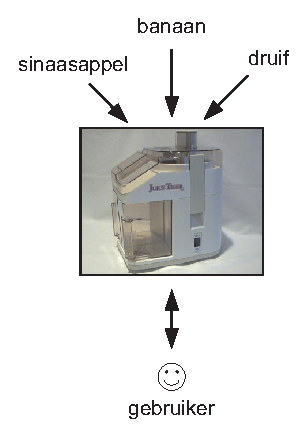
\epsfig{file=pics/eps/sapcentrifuge.eps, height=6cm}
      \caption{Een generieke sapcentrifuge.}\label{genericJuicer} 
    \end{center}
  \end{minipage}
\hfill
\begin{minipage}[b]{.47\textwidth}
    \begin{center}  
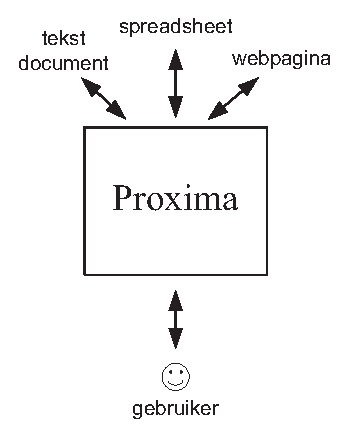
\epsfig{file=pics/eps/generiekeEditor.eps, height=6cm}
      \caption{Een generieke editor.}\label{genericEditor} 
    \end{center}
  \end{minipage}
\end{figure}


Gerelateerd aan dit onderscheid tussen edit-operaties kunnen bestaande generieke editors in twee categorie\"en ingedeeld worden. Aan de ene kant zijn er de {\em syntax-directed} editors, die een krachtig presentatiemechanisme kunnen bieden, maar vrijwel alleen documentgerichte edit-operaties bieden. Dit wordt door gebruikers vaak als beperkend  ervaren. De andere categorie wordt gevormd door de {\em syntax-recognizing} editors. Deze editors staan het vrij editen van de presentatie toe, maar beschikken weer over een beperkt presentatiemechanisme. Er bestaan ook tussenvormen ({\em hybrid} editors), maar die zijn vrijwel altijd te beschouwen als hoofdzakelijk syntax-directed danwel syntax-recognizing editors.

%Gebruiksvriendelijker zijn de presentatiegerichte generieke editors, die toestaan dat de presentatie van het %document op het scherm ge�dit kan worden. Deze editors zijn echter slechts toepasbaar voor een beperkte %klasse, veelal tekstuele, documenttypes.

\bc
generieke editors de naam gebruiksonvriendelijke applicaties te zijn met een beperkte toepasbaarheid. Een belangrijke eigenschap van Proxima is dat de editor presentatiegericht is; edit operaties kunnen worden uitgevoerd op wat op het scherm zichtbaar is, in plaats van op de interne structuur van het document. Tegelijkertijd is het ook nog steeds mogelijk om de onderliggende structuur zichtbaar te maken en te wijzigen, vergelijkbaar met het onderwaterscherm van wordperfect.
\ec


%Onderzoek hoe voordelen van documentgericht editen met presentatie gericht editen.
In dit proefschrift onderzoeken we hoe de voordelen van een generieke editor met een krachtig presentatiemechanisme te combineren zijn met een presentatiegericht edit model. 

% inventarisatie?
%Na een introductie van relevante begrippen en verschillende soorten editors in %Hoofdstuk~\ref{chap:introduction} wordt in 

Na een algemene inleiding en een introductie van relevante begrippen in Hoofdstuk~\ref{chap:introduction},
wordt in Hoofdstuk~\ref{chap:requirements} een aantal uiteenlopende toepassingen van een generieke editor beschreven.  Onder deze voorbeelden bevinden zich bekende applicaties als een editor voor programmacode, een tekstverwerker en een formule editor, maar bijvoorbeeld ook een elektronisch belastingformulier. Tezamen helpen de voorbeelden het toepassingsgebied van de Proxima editor vast te leggen. Aan de hand van de voorbeelden, die elk hun specifieke eisen stellen aan de editor, formuleren we een zestal functionele eisen, of requirements, voor een generieke editor: 
% waar een generieke editor aan zou moeten voldoen om de voorbeeld editors te kunnen implementeren:
% pres-oriented doc-oriented


%beetje afstand fruiteditor: we willen de presentatie editen. Hiervoor word het presentatie process opgesplitst %in stappen. Het terugvertalen wordt daardoor eenvoudiger. De stappen zijn gebaseerd op het presentatieproces. %niveaus (levels) lagen (layers)

\begin{description}
\item [Genericiteit.] Uitgangspunt van het onderzoek is dat de editor generiek is, en niet ontworpen voor een specifiek documenttype.
\item [Berekeningen in de presentatie.] De presentatie moet berekende waarden en structuren kunnen bevatten, zoals hoofdstuknummers en een automatische inhoudsopgave.
\item [Krachtig grafisch presentatieformalisme.] Het presentatieformalisme moet krachtig genoeg zijn om tekstverwerkingsdocumenten met wiskundige formules te tonen, maar ook  een elektronisch formulier met invoervelden en knoppen.
%A graphical presentation language with a powerful mapping formalism.]
\item [Presentatiegericht en documentgericht editen.] Edit-operaties op zowel het document als op de presentatie moeten ondersteund worden. Tevens moeten edit-operaties voor specifieke documentsoorten gespecificeerd kunnen worden.
%Niet restrictief, pres editen. Tegelijkertijd ook mogelijk om aan de hand van
% de interne structuur (bv 2 hoofdstukken verwisselen)
\item [Modeless editen.] Het moet het mogelijk zijn om eenvoudig te wisselen tussen presentatiegericht en documentgericht editen, zonder de editor expliciet in een andere toestand (mode) te moeten brengen.
%Modeless editing.]
\item [Extra state.] In sommige gevallen bevat een document informatie die niet in de presentatie zichtbaar is, en soms bevat de presentatie weer informatie die niet in het document opgeslagen is. Deze informatie noemen we {\em extra state}. De editor moet beide vormen van extra state ondersteunen.
%Support for presentation extra state as well as interpretation extra state.
\end{description}

\bc
\begin{figure}
\begin{center}
bla %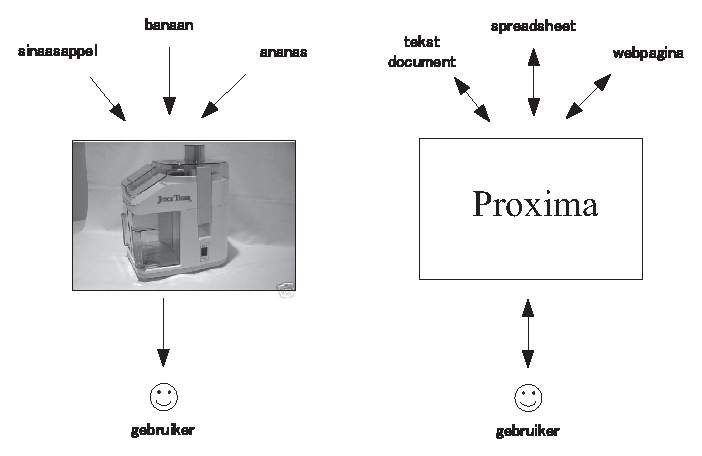
\epsfig{file=pics/eps/juicerVSeditor.eps, height=6cm}
\end{center}
\caption{Twee vormen van genericiteit.} \label{genericity}
%andere caption: Juice Tiger vs. Proxima. ?
\end{figure}
\ec



Aan de hand van bovenstaande requirements wordt een aantal bestaande systemen onder de loep genomen en met elkaar vergeleken. Het blijkt dat geen van de bestaande systemen aan alle requirements voldoet, wat betekent dat er dus geen systeem is dat alle voorbeelden kan ondersteunen. E\'en van de problemen is dat een editor aan de ene kant moet beschikken over een krachtig  presentatiemechanisme met ondersteuning voor berekende waarden, grafische elementen en eventuele duplicatie van informatie. Aan de andere kant moet voor een gebruiksvriendelijk edit model het editen van de presentatie mogelijk zijn. Dit laatste houdt echter in dat een gewijzigde presentatie terugvertaald (ge\"\i nterpreteerd) moet worden naar een nieuw document, wat moeilijker is naarmate het presentatiemechanisme complexer is. 
% en duplicaten mag bevatten

%%%%%%%%%%%%%%%% 
\bc Proxima is een presentatiegerichte editor die complexe presentaties met grafische elementen en berekende waarden ondersteunt, en daarom bruikbaar is voor een grote klasse van documenttypes.  \ec
In hoofdstuk~\ref{chap:proxArch} stellen we een gelaagde architectuur vast, voor een editor die voldoet aan de zes requirements. Het probleem om presentatiegerichte editfunctionaliteit te bieden wordt door de gelaagde architectuur opgesplitst in een aantal eenvoudigere deelproblemen. De lagen vinden hun oorsprong in het presentatie proces dat in een aantal logische stappen verdeeld kan worden. Voorbeelden van deze stappen zijn het berekenen van afgeleide waarden, het bepalen van de logische opmaak van de presentatie, tot aan het uitrekenen van alle posities en het tonen van de presentatie aan de gebruiker. Het interpretatie proces doorloopt dezelfde stappen in omgekeerde volgorde. Elk van de tussenresulaten wordt een data-niveau of {\em level} genoemd. Tussen twee niveaus bevindt zich een laag (of {\em layer}) die waarden van het ene niveau op het andere afbeeldt in zowel de presentatie als interpretatie richting.
%Eerst worden aan het document berekende waarden toegevoegd, zoals hoofdstuknummers een inhoudsopgave. Het %resultaat hiervan is de enriched document. De enriched document wordt vervolgens afgebeeld op de presentation. %Sommige documentpresentaties hebben layout informatie die niet in het document opgeslagen is (extra state), %deze wordt. Ten slotte wordt de arrangement afgebeeld op een rendering.
Het hoofdstuk geeft een overzicht van de verschillende data-niveaus en de lagen daartussen. De presentatie en interpretatie processen worden beschreven met behulp van voorbeelden. 

Hoofdstukken~\ref{chap:informalSpec} en~\ref{chap:formalSpec} geven een specificatie van de Proxima editor. Hoofdstuk~\ref{chap:informalSpec} is een inleiding op de specificatie, en geeft een model van het edit proces. Ook worden de begrippen extra state en duplicaten in de presentatie beschreven. De specificatie zelf is het onderwerp van Hoofdstuk~\ref{chap:formalSpec}. Het uitgangspunt is dat, gegeven een presentatiefunctie, een corresponderende interpretatiefunctie gespecificeerd wordt. De specificatie wordt in een aantal stappen ontwikkeld. De eerste stap is de specificatie van een editor die uit slechts \'e\'en laag bestaat en geen rekening houdt met extra state. Deze specificatie wordt vervolgens stap voor stap uitgebreid tot de specificatie van een gelaagde editor met ondersteuning voor extra state. Het hoofdstuk eindigt met een schets van de behandeling van presentaties die duplicaten kunnen bevatten.


\bc In Chapter~\ref{chap:presenting}, we discuss the {\Xprez} presentation formalism of the Proxima. {\Xprez} is a declarative presentation language, suited for specifying a wide range of presentations. We state a number of requirements for a presentation language for structured documents, and provide an informal overview of {\Xprez}, using a series of examples. \ec

Om een document af te beelden op het scherm maakt Proxima gebruik van de presentatietaal {\Xprez}. {\Xprez} is een declaratieve presentatietaal die geschikt is voor een verscheidenheid aan toepassingen. Hoofdstuk~\ref{chap:presenting} inventariseert een aantal requirements voor een presentatietaal en bevat een vergelijking van een aantal van zulke talen. Vervolgens wordt aan de hand van voorbeelden een informele beschrijving van de taal {\Xprez} gegeven.

Hoofdstuk~\ref{chap:prototype} beschrijft het prototype van Proxima, dat is ge\"\i mplementeerd in de functionele programmeertaal Haskell en voldoet aan de zes genoemde requirements. De berekende waarden en de presentatie van het document worden gespecificeerd met behulp van een attributengrammatica, terwijl de interpretatie richting met een combinator parser beschreven wordt. Het hoofdstuk toont screenshots van het prototype en bevat ook een aantal voorbeelden van de style sheets waarmee specifieke editors beschreven worden.

Ondanks de nog prille staat van het prototype is het al mogelijk om met relatief weinig moeite complexe editors te bouwen die toch prettig in het gebruik zijn. Op basis van de ervaringen met  het prototype kunnen we concluderen dat de combinatie van een krachtig presentatiemechanisme en een presentatiegericht edit model zeker mogelijk is.
% editor



\bc Even without the language support and libraries for common presentation patterns, it is already straightforward to specify a complex editor in Proxima. Thus, the Proxima prototype shows that it is possible to combine a powerful presentation formalism with a modeless integration of document-oriented and presentation-oriented editing. The resulting editors are powerful, yet easy to use.
\ec

%arch maakt het mogelijk om concise editors te specificeren die presentatie en doc combineren.

%\todo{AG}\todo{parser combinators}

\bc A prototype that offers much of the functionality discussed in this thesis has been implemented in the functional language Haskell. Chapter~\ref{chap:prototype} discusses the prototype as well as a number of editors that have been instantiated. The chapter also explains which components need to be provided to instantiate an editor. \ec

%Hoofdstuk~\ref{chap:conclusions}


\bc
Chapter~\ref{chap:requirements} explores applications of generic structure editing by providing five use cases of real-world editors. With these use cases in mind, we formulate a number of functional requirements that in our view are important for a flexible non-restrictive structure editor. We evaluate a number of existing editors according to the requirements, and conclude with an overview of how the Proxima editor is designed to meet the requirements and be able handle all use cases.

The layered architecture of Proxima is introduced in Chapter~\ref{chap:proxArch}.  The chapter discusses the various data levels, as well as the layers that maintain the mappings between the levels. The discussion is illustrated with examples of the presentation and interpretation processes.

In chapters~\ref{chap:informalSpec} and~\ref{chap:formalSpec}, we develop a specification of the Proxima editor. Chapter~\ref{chap:informalSpec} serves as an introduction to the specification and introduces our model of the edit process, as well as the concepts of extra state and duplicates in the presentation. In  Chapter~\ref{chap:formalSpec}, we start by specifying a simple editor, to which extra state and multiple layers are added in subsequent sections. The chapter ends with an informal discussion on how to handle presentations that contain duplicates.

In Chapter~\ref{chap:presenting}, we discuss the {\Xprez} presentation formalism of the Proxima. {\Xprez} is a declarative presentation language, suited for specifying a wide range of presentations. We state a number of requirements for a presentation language for structured documents, and provide an informal overview of {\Xprez}, using a series of examples.

A prototype that offers much of the functionality discussed in this thesis has been implemented in the functional language Haskell. Chapter~\ref{chap:prototype} discusses the prototype as well as a number of editors that have been instantiated. The chapter also explains which components need to be provided to instantiate an editor.

Finally, Chapter~\ref{chap:conclusions} presents the conclusions and gives an overview of future work.

\ec





%%%%%%%%%%%%%

\bc
Aanmelden Promotie

\head{Onderwerp promotieonderzoek}

Presentatiegericht editen van gestructureerde documenten en XML.

(bijvoorbeeld: 'Botontkalking bij de labrador' of 'Leerachterstand allochtone kleuters')
   
\head{Belangrijkste conclusie(s)}

Door gebruik te maken van een gelaagde architectuur is het mogelijk om een presentatiegerichte generieke editor te bouwen die geschikt is voor een breed scala aan toepassingen. 


\head{Belangrijkste aanbeveling(en)}
\ec
\selectlanguage{dutch}
\chapter*{Curriculum Vitae}
\label{chap:cv}
\addcontentsline{toc}{chapter}{Curriculum Vitae}

Martijn Michiel Schrage

\subsubsection*{4 juni 1973}
Geboren te Veendam.

\subsubsection*{augustus 1986 -- juni 1991}
Athenaeum op een heleboel verschillende scholen.

\subsubsection*{september 1991 -- februari 1997}
Studie Informatica aan de Universiteit Utrecht.

\subsubsection*{april 1997 -- februari 1999}
Wetenschappelijk medewerker bij het Skit-project aan het Informatica-instituut van de
Universiteit Utrecht.

\subsubsection*{september 1999 -- augustus 2003}
Assistent in Opleiding aan het Informatica-instituut van de
Universiteit Utrecht.




\thispagestyle{empty}
\cleardoublepage
\end{document}
